\documentclass[12pt]{book}
\usepackage[utf8]{inputenc}
\usepackage{graphicx}
\usepackage{amsmath}
\usepackage{amssymb}


\title{Peculiaridades del Tono del Violín}
\author{Frederick Castle, M. D.}
\date{1906}

\begin{document}

\maketitle
\begin{center}
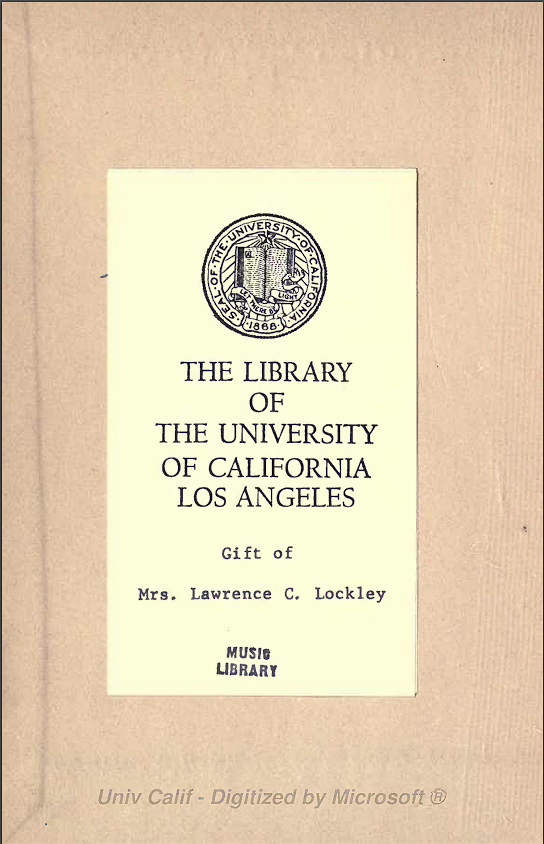
\includegraphics[width=1\textwidth]{./img/portada.png} % Reemplaza "imagen.jpg" con el nombre del archivo de la imagen
\end{center}
\begin{center}
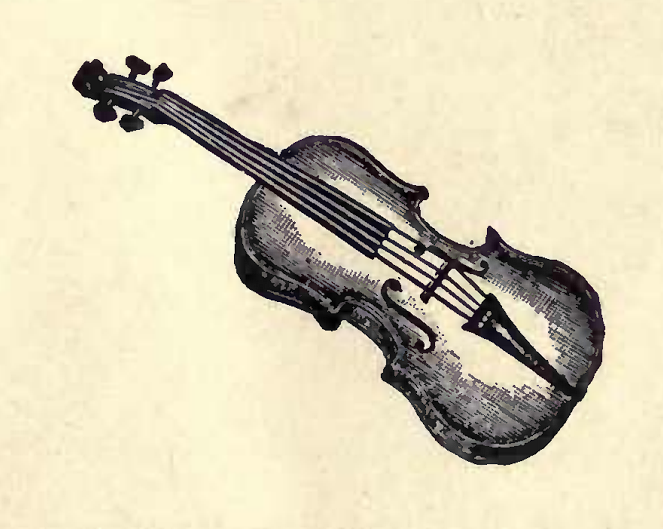
\includegraphics[width=0.5\textwidth]{./img/violin.png} % Reemplaza "imagen.jpg" con el nombre del archivo de la imagen
\end{center}

\begin{center}
\textbf{LOWELL, INDIANA.\\
Alfred Ha Miller}

\textbf{Copyright 1906,\\
Por Frederick Castle, M. D.\\
H. H. RAGON \& SON, Impresores,\\
Lowell, Indiana.\\
1906.}
\end{center}

\begin{center}
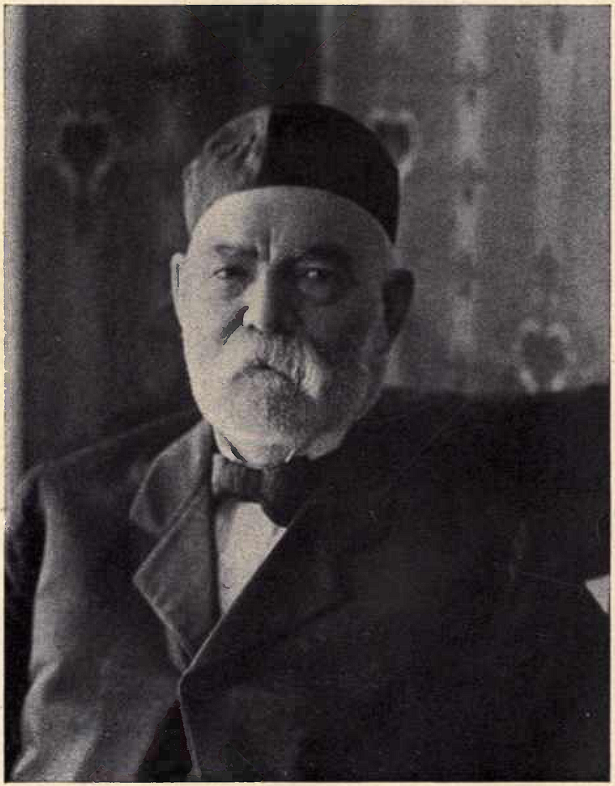
\includegraphics[width=1\textwidth]{./img/foto.png} % Reemplaza "imagen2.jpg" con el nombre del archivo de la imagen
\end{center}

\chapter*{Agradecimientos}

Es gratificante reconocer al Mayor Gilbert Thompson, Washington, D. C., y al Sr. Frank Spalding, Director del Municipio de Griffth, Indiana, como personas que brindaron una valiosa ayuda para hacer que este libro sea presentable.

\begin{flushright}
\textbf{FREDERICK CASTLE}
\end{flushright}

\chapter*{Explicación del Gráfico}

Debido a que diferentes muestras de madera para la tapa armonica deben recibir un tratamiento distinto en cuanto a graduación, no se dan valores para los espesores; pero en lugar de cifras, se emplea sombreado como medio para indicar valores cuantitativos relativos. El único experimento anotado en el texto, y que tiene en cuenta la uniformidad máxima del poder tonal, operó para aumentar las notas altísimas en un grado más marcado que los tonos de menor altura. Debido a que el poder en los tonos altísimos es deseable y difícil de asegurar, por lo tanto, se registra este método de graduación, con la esperanza de que futuros estudiantes del violín continúen experimentando con el acortamiento de la longitud de la actividad de la tapa armonica para aumentar los tonos de mayor altura. La prueba sin duda determinará una mejor proporción que 2-3 para acortar la actividad de las fibras bajo las cuerdas más ligeras.

\begin{center}
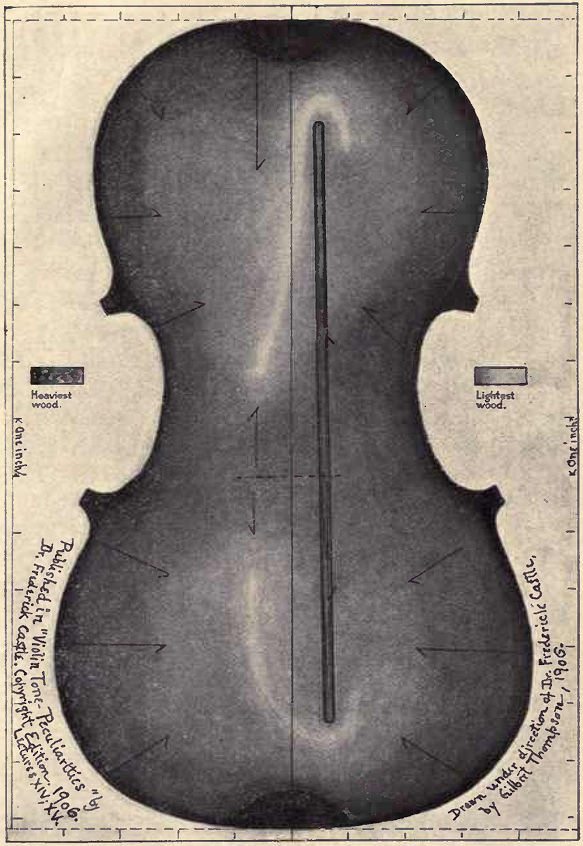
\includegraphics[width=1\textwidth]{./img/grafico.png} % Reemplaza "grafico.jpg" con el nombre del archivo de la imagen
\end{center}

\chapter*{Contenido}

\begin{itemize}
    \item \textbf{GRÁFICO} ... 6
    \item \textbf{ÍNDICE} ... 8
    \item \textbf{INTRODUCCIÓN} ... 12
    \item \textbf{CONFERENCIA I—Carácter del Tono del Violín} ... 17
    \item \textbf{CONFERENCIA II—Accidente Nº 1} ... 26
    \item \textbf{CONFERENCIA III—El Constructor de Violines Fraudulento} ... 42
    \item \textbf{CONFERENCIA IV—Madera de la tapa armonica del Violín} ... 57
    \item \textbf{CONFERENCIA V—Desintegración de las Superficies Interiores del Violín} ... 78
    \item \textbf{CONFERENCIA VI—Mi Violín Desgastado, o Fenómeno del Barniz Nº 1} ... 92
    \item \textbf{CONFERENCIA VII—Fenómeno del Barniz Nº 2} ... 113
    \item \textbf{CONFERENCIA VIII—Uniformidad de los Valores del Violín} ... 130
    \item \textbf{CONFERENCIA IX—Modificadores del Tono del Violín} ... 150
    \item \textbf{CONFERENCIA X—Modificadores del Tono del Violín, continuación} ... 160
    \item \textbf{CONFERENCIA XI—Modificadores del Tono del Violín, continuación} ... 171
    \item \textbf{CONFERENCIA XII—Modificadores del Tono del Violín, continuación} ... 180
    \item \textbf{CONFERENCIA XIII—Modificadores del Tono del Violín, continuación} ... 190
    \item \textbf{CONFERENCIA XIV—Uniformidad Máxima del Poder Tonal del Violín} ... 205
    \item \textbf{CONFERENCIA XV—Uniformidad Máxima del Poder Tonal del Violín, conclusión} ... 222
    \item \textbf{CONFERENCIA XVI—Poder Tonal Máximo del Violín} ... 235
    \item \textbf{CONFERENCIA XVII—Filosofía Relacionada con las Condiciones de las Superficies Interiores del Violín} ... 256
    \item \textbf{CONFERENCIA XVIII—Nuestro Pasar} ... 274
    \item \textbf{APÉNDICE} ... 289
\end{itemize}

\chapter*{Índice}

\begin{itemize}
    \item \textbf{ACCIDENTE Nº 1} ... 26
    \item \textbf{SONIDO AUDIBLE} limitado a doce pulgadas de la tapa armonica del violín, 53
    \item \textbf{ÁNGULOS} incidencia y reflexión, 304
    \item \textbf{LIBROS} evidencia poco confiable en, 35
    \item \textbf{MEJOR VIOLÍN SOLISTA} no el mejor violín de orquesta, 37
    \item \textbf{PLACA POSTERIOR} funciones de, 47; como un agente productor de tono, 107
    \item \textbf{CUIDADO DEL BARNIZ} ejemplo, 93
    \item \textbf{BARNIZ DE CREMONA} 125
    \item \textbf{EFECTO TONAL COMBINADO} media docena de violines de tono uniforme, 136; condiciones de la prueba, 136
    \item \textbf{TONO FRÍO} 296
    \item \textbf{SOBRETONOS DISONANTES} causa de, 30; 295
    \item \textbf{FRAUDE} 43
    \item \textbf{PROPÓSITO GENERAL} Violín, 38
    \item \textbf{GOMAS} duras, inelásticas, efecto de, 93
    \item \textbf{EL GUSHER} 285
    \item \textbf{ARMÓNICOS} valor de, 96
    \item \textbf{SOBRETONOS ARMÓNICOS} 294
    \item \textbf{INTRODUCCIÓN XII} método de llegar a conclusiones, xiv, ocho proposiciones, xv
    \item \textbf{INSENSATEZ} continuar la demanda de que solo aparezcan solistas con un Stradivarius o un Guarnerius, 39
    \item \textbf{INVITACIÓN} a mi violín de pastor, 101
    \item \textbf{LONGEVIDAD} del violín, 98; ejemplo, 98
    \item \textbf{PÉRDIDA DE PODER TONAL} causas de, 299
    \item \textbf{CONDICIONES METEOROLÓGICAS} 23
    \item \textbf{SONIDO MUSICAL} ley explícita, 30; afectando la distancia recorrida por el tono del violín, 280
    \item \textbf{UNIFORMIDAD MÁXIMA} del poder tonal del violín, 205; tonos fundamentales, 208; razones que conducen a un nuevo método para la graduación de la tapa armonica, 214; demostración de áreas de la tapa armonica que aumentan el tono de cada cuerda, 216; proporción para las longitudes de actividad de las fibras debajo de cada cuerda, 218; afinación de concierto hace 200 años, 223; demostración de que los errores en la graduación de la tapa armonica causan poder tonal desigual, 225
    \item \textbf{PODER TONAL MÁXIMO} 235; "gran" tono, 236; el tono del violín separado por dos factores irreconciliables, 237; esteticismo del violín llevado al extremo, 238; lista de factores que producen el poder tonal máximo del violín; apariencias físicas de la madera de la tapa armonica que produce un poder tonal máximo combinado con tono "rico", 246; vibración normal y transversal en la tapa armonica, 249; tono amaderado, 255; dispersión de la fuerza, la pelota rebotando, 271
    \item \textbf{RUIDO} definición de, 25
    \item \textbf{NODOS} 294
    \item \textbf{OH, TÚ POSTE} 276
    \item \textbf{TONO} Sonido musical, 30
    \item \textbf{INTÉRPRETES} Opiniones variadas de, 36
    \item \textbf{FILOSOFÍA} Involucrada en las condiciones de las superficies interiores del violín, 256; lista de principios que modifican el tono del violín, 259; número de cualidades tonales absolutamente al alcance del constructor de violines, 261; intensidad del tono del violín producto de cuatro factores, 262; propiedades del aire que afectan la intensidad del tono del violín, 264
    \item \textbf{PENETRACIÓN} del aceite, 274
    \item \textbf{PASAR} 276
    \item \textbf{POSTE} problema del, 301
    \item \textbf{TONO RICO} causas de, 96; descripción de la madera rica en tono, 97; ilustración, 296
    \item \textbf{CIENCIA} nunca hizo un violín, 32
    \item \textbf{DECLARACIONES CIENTÍFICAS} recibidas con precaución, 32
    \item \textbf{MADERA DE LA tapa armonica} 57; contribución de la ciencia, 58; valor en escrutinio de la madera usada, 61; violines desiguales, encogimiento, ejemplo, 62; ejemplo, 63; fallas del pino, 66; pino de Michigan, 67; cedro blanco, 69; cambios de color en el pino, 70, acción independiente de fibras contiguas, 71; patético, 78; preservando superficies interiores, 79; ejemplo de desintegración de superficies interiores, 83
    \item \textbf{ACCIÓN SIMPÁTICA} 108; ley de, 109
    \item \textbf{VIOLÍN ANTIGUO Y DULCE} 91
    \item \textbf{EL REY} 20
    \item \textbf{DOS ERRORES} 22
    \item \textbf{PRUEBA DE DISTANCIA DE TONO} al aire libre, 23; el oído escuchando en la mejor posición, 24
    \item \textbf{PROMOTORES DEL COMERCIO} industria de, 39
    \item \textbf{EL HOMBRE DE DOS DÓLARES} 41
    \item \textbf{TÚ, OH VIOLÍN} 45
    \item \textbf{ALTURA DEL TONO} 45; ocho reglas de aplicación, 48; regla 2, 48; regla 3, 49; regla 4, 49; regla 5, 50; regla 6, 50; regla 7, 51; regla 8, 51
    \item \textbf{MODIFICADORES DEL TONO} lista, 141; barniz, 142; doblado de la tapa armonica, 143; doblado de la parte posterior, 144; espesor de la tapa armonica, 144; arqueado, 147; arqueado alto, ejemplo, 148; leyes que gobiernan las líneas de viaje de las ondas sonoras, 151; problema no resuelto en el arqueado, 152; la barra, 152; lobo causado por mala posición de la barra, 153; lobo causado por la graduación, 154; posición de la barra disminuyendo el poder de la cuerda D, 158; el poste, 160; el puente, 164; el diapasón, 165; las cuerdas, 181; bloque de refuerzo, 175; el violín tembloroso, 181; superficies interiores, 185; las salidas, 187; profundidad de las costillas, 199; la sordina, 302; crines del arco, 202
    \item \textbf{UNIFORMIDAD} de los valores tonales del violín, 131
    \item \textbf{VEREDICTO} Etiqueta, Barniz y Precio vs Tono Dulce, 305
    \item \textbf{CARACTERÍSTICAS DEL TONO DEL VIOLÍN} lugar de utilidad, 19
    \item \textbf{TRABAJOS DE CHAPADO} 53
    \item \textbf{FENÓMENO DEL BARNIZ Nº 1} 104
    \item \textbf{FENÓMENO DEL BARNIZ Nº 2} 113
    \item \textbf{VIBRACIÓN} normal y transversal, 291; velocidad comparada, 299
    \item \textbf{SEGMENTOS VENTRALES} 295
    \item \textbf{LOBO} causado por la barra, ejemplo, 153; causado por la graduación de la tapa armonica, ejemplo, 154
\end{itemize}

\chapter*{Fe de Erratas}

\begin{itemize}
    \item Página 19, línea 8, en lugar de "tenora," lea tenoro.
    \item Página 44, línea 2 verso, en lugar de "Music," lea Music's.
    \item Página 48, línea 12, en lugar de "give," lea gives.
    \item Página 57, línea 24, en lugar de "govern's," lea governs.
    \item Página 96, línea 14, en lugar de "a basso," lea a bassa.
    \item Página 173, línea 1, en lugar de "diminish," lea increase.
    \item Página 216, línea 20, en lugar de "purfing," lea purfling.
    \item Página 217, líneas 1, 13, en lugar de "purfing," lea purfling.
    \item Página 297, línea 3, en lugar de "MOVEMENT," lea MOVEMENTS.
\end{itemize}

\chapter*{Introducción}

Estas conferencias, dirigidas a una audiencia imaginaria de estudiantes de violín, fueron originalmente escritas y parcialmente publicadas en el Western Musician, Dixon, Illinois, para el entretenimiento de los numerosos lectores de esta revista musical. Dos de las conferencias ahora aparecen impresas por primera vez. Como se empleó un estilo familiar, se evitaron términos técnicos abstractos en la medida de lo posible sin interferir con la claridad y precisión.

Los experimentos, resultados y conclusiones, tal como se registran aquí, no son fantasías de la imaginación, como podría inferirse al principio, sino que son conclusiones obtenidas a través de experimentos prácticos, y también por accidentes ocurridos en mi experiencia.

Así, cuando pacientes violines llegaron a mi hospital, me sentí feliz, y debido a mi entusiasta devoción a los problemas de diagnóstico tonal, trabajé sobre ellos, y sobre ellos, hasta declararlos curados o incurables. Algunos de esos pacientes violines eran, como algunos pacientes humanos, bendecidos con buenas constituciones inherentes desde el principio, y eran capaces de recibir valores tonales mejorados a partir del ajuste cuidadoso de los factores modificadores del tono, mientras que otros eran tan inherentemente malos desde el día en que fueron llamados "violín" (mal llamados), que solo heredaron un tono ruidoso; sin embargo, el tono ruidoso hizo "casos interesantes" de esta última clase debido a que ofrecían razones incontrovertibles para el tono inferior, razones que demostraban concluyentemente la verdad en la afirmación "sin material superior, sin violín superior."

Durante mi periodo de trabajo activo, siempre tuve en mente las siguientes preguntas:
\begin{itemize}
    \item "¿Cómo opera el violín para producir sonido musical?"
    \item "¿Qué agentes, conectados con el violín, operan para modificar el tono?"
    \item "¿Cuáles son las causas del tono inferior en un violín?"
    \item "¿Cuáles son las causas del tono superior en un violín?"
\end{itemize}

Algunas de estas preguntas las he resuelto a mi satisfacción, pero no pretendo que tales soluciones sean aceptables para otros estudiantes de fenómenos tonales del violín; ni pretendo que todos esos problemas de tono hayan recibido solución. Algunas de mis conclusiones están en desacuerdo con las conclusiones de investigadores científicos notables, pero no reclamo infalibilidad para mis propias conclusiones. Errar es humano. Seguir el error también es humano. Así, seguí una conclusión científica sobre la producción y modificación del tono del violín que requirió experiencias de veinticinco años para disipar la ilusión. Sobre esta base, se advierte al estudiante de violín sobre el peligro de seguir teorías abstractas bajo el disfraz de la ciencia.

Creo que las teorías, incluso cuando se basan en demostraciones prácticas repetidas en varios violines, deben presentarse solo como conclusiones de un individuo que intenta resolver un problema en el que la acción caprichosa de la madera ha sido, es y siempre puede seguir siendo una cantidad desconocida; y presento la idea de que tal cantidad desconocida es la razón por la cual la ciencia fracasa al intentar construir un violín por encargo.

Los siguientes problemas permanecen sin elucidación:
\begin{itemize}
    \item "Acción caprichosa inherente de la madera."
    \item "Diferentes grados de concentración de ondas sonoras en las salidas según diferentes grados de arqueado de las placas."
    \item "El fenómeno de elevar la altura tonal al agrandar el área de las salidas."
\end{itemize}

Se presenta la opinión de que las soluciones para los dos primeros problemas pondrán la calidad tonal del violín bajo el control de la voluntad. No obstante, a pesar de las dudas de resolver los problemas involucrados en la acción caprichosa de la madera, el valor de tal solución sigue siendo un incentivo poderoso para continuar el esfuerzo. El deseo de violines que posean un tono "rico" combinado con una marcada intensidad de tono es un estímulo que supera el estímulo del oro fino; y quien descubra un método para producir tales violines a voluntad se convertirá en un rey en su propio derecho.

Mi método para llegar a conclusiones sobre la potencia de cada modificador del tono del violín es investigar las causas del tono ruidoso, tono dulce, tono poderoso, tono hueco, tono fino, tono "todo por dentro", tono "todo por fuera", volumen de tono, intensidad del tono, altura tonal, tonos dobles no musicales, tonos abiertos poderosos con tonos altísimos débiles, tonos resultantes o armónicos a bassa, sobretonos consonantes, sobretonos disonantes, el "tono rico", el "tono frío", tono simpático, uniformidad del poder tonal, y carácter tonal basado en el carácter tonal de la voz humana.

En este trabajo, las conclusiones aquí presentadas siguen experimentos realizados tanto en violines antiguos como nuevos, y el número de tales violines asciende a cientos. A partir de las deducciones así obtenidas, mi deseo es dar prominencia a las siguientes proposiciones:
\begin{itemize}
 \item Las peculiaridades tonales que existen en un violín dado pueden no existir en ningún otro violín.
 \item Escribir sobre peculiaridades tonales que existen en un violín dado como necesidades infalibles para todos los violines es engañoso.
 \item Encontrar dos violines que posean valores tonales precisamente similares es igualmente difícil que encontrar dos voces que posean valores tonales precisamente similares.
 \item Ningún fabricante de violines, sea quien sea, ha sido capaz de otorgar un valor tonal destacado a cada violín.
 \item Que el pastor de ovejas de la montaña puede producir un violín con valores tonales iguales a los mejores.
 \item Que el mecánico hábil, guiado por un instinto musical infalible, produce un número vastamente mayor de violines superiores que el mecánico sin tal instinto.
 \item Que todos los fabricantes de violines pueden experimentar derrotas ocasionales.
 \item Que, salvo accidente, el violín superior es producto de una habilidad mecánica superior combinada con un sentido musical superior, todo dirigido sobre material superior.
\end{itemize}
No parece haber otro método que ofrezca un valor igual a las conclusiones que el método aquí presentado para determinar la potencia y operación de cada factor que interviene en la producción y modificación del tono del violín.

A la evaluación de tales factores he dedicado una vida; no en teorías abstractas, sino sentado en el banco mientras repetía demostración tras demostración, año tras año, década tras década, desde la juventud hasta la vejez, decidido a aislar, evaluar y conocer la operación de todos y cada uno de los factores subyacentes en los fenómenos tonales del violín, o morir en el intento. A los sesenta y tres años, la muerte estuvo cerca, y tres años después siguió cerca, dejando solo mi brazo derecho suficientemente útil para guiar la pluma. Ahora es seguro que no alcanzaré la meta de mi ambición.

Bajo tales dificultades, escribir es laborioso; además, el material aquí presentado se compone completamente de memoria, no se tomaron notas con vistas a la publicación. En el momento presente, la conservación necesaria de fuerzas me limita a un período diario limitado de trabajo; por lo tanto, abandono la reescritura planeada de la publicación preliminar, de la cual se hicieron las correcciones necesarias, y de la cual se omiten algunos párrafos, y a la cual se agregan las conferencias xvi y xvii. Esta publicación se presenta como mi legado tanto para el estudiante de violín como para el fabricante de violines estadounidense. Que el siguiente registro se reduzca a la escritura y se publique es algo debido enteramente al estímulo ofrecido por un fabricante de violines moderno; por lo tanto, cualquier entretenimiento o cualquier otro valor que se pueda encontrar en estas páginas es algo no atribuible únicamente al coraje de, FREDERICK CASTLE. Lowell, Indiana, 20 de marzo de 1906.

\chapter*{Conferencia I}
SEÑORES ESTUDIANTES DEL VIOLÍN, en esta, nuestra primera sesión, aprovecho la oportunidad para ofrecerles mis felicitaciones por los siguientes hechos interesantes. Primero: se han descubierto las causas del tono ruidoso en los violines. Segundo: se ha perfeccionado una forma exitosa de preservar las superficies interiores del violín de la desintegración por el calor y la humedad. Tercero: las áreas de la tapa armonica del violín, responsables de la producción y aumento del tono, han sido localizadas y definidas. Cuarto: se ha demostrado un método de graduación de la tapa armonica que asegura la máxima uniformidad en el poder tonal. Quinto: los principios que rigen la intensidad del tono del violín han salido a la luz. Sexto: los principios que gobiernan el poder del tono del violín se han expresado en palabras. Séptimo: se ha descrito la calidad de la madera de la tapa armonica que permite obtener un "tono rico" en el violín. Octavo: se ha registrado el poder del accidente para disipar la oscuridad y la ilusión. Noveno: algunas conclusiones científicas sobre "cómo opera el violín para producir sonido musical" han sido sacudidas. Décimo: se ha demostrado la falacia en la afirmación de que "los mejores Cremonas son vehículos necesarios para la interpretación de las partituras de Haydn, Mozart y Beethoven". Undécimo: se ha intentado corregir los agravios impuestos al fabricante de violines moderno por el "promotor del comercio de violines antiguos".

Durante nuestro curso de estudio, se les presentarán algunas ideas sobre el tono del violín que hasta ahora no se han expresado. De hecho, les prometo que habrá muy poco contenido repetido en nuestro menú. Como no es mi intención privarlos del placer que ofrece la anticipación, solo se les darán pequeñas dosis a la vez. Este plan se adopta para evitar dañar su capacidad de digestión y para asegurar su asistencia regular.

El gusto por el tono varía—varía a través de cada grado de cultura musical. Un tono que agrada a una persona puede no agradar a otra. Ningún intérprete puede tocar al máximo en un instrumento cuyo tono le resulte desagradable. Afortunadamente, el violín ofrece una variedad de calidad tonal tan infinitamente grande que cada violinista en la Tierra puede poseer uno con una calidad tonal que se ajuste a su gusto.

Uno podría pensar que es posible fabricar violines con un estándar único de calidad tonal, pero el hecho es que la peculiaridad inherente de la acción de la madera lo impide.

Existe algo que se aproxima a un estándar tonal invariable para toda la gama de instrumentos de viento e instrumentos de percusión.

Pero la calidad tonal invariable se detiene abruptamente ante la presencia de la familia del violín. Podemos imaginar la inmensa sorpresa de alguien que nunca ha escuchado otros instrumentos que no sean de viento al ser introducido a esta familia de violines. A medida que toma violín tras violín, viola tras viola, violonchelo tras violonchelo, no encuentra dos que posean un carácter tonal idéntico. Cada violín, cada viola, cada violonchelo tiene una calidad tonal peculiar a sí mismo. Estas peculiaridades son tan marcadas que pronto se vuelve capaz de nombrar cada violín con cuyos tonos está familiarizado, aunque esté con los ojos vendados o en una habitación distante, nombrándolos con la misma certeza con la que puede identificar diferentes cantantes con cuyos tonos está familiarizado.

Se vuelve curioso por conocer la razón o las razones de la infinita peculiaridad tonal de ese maravilloso instrumento musical llamado "violín".

Por observación, descubre que las cuerdas G y D a veces poseen un carácter tonal grave; en otros momentos, estas cuerdas poseen un carácter barítono-tenor; en algunos casos, las cuerdas A y E poseen un carácter mezzo-soprano; en otros casos, las cuerdas A y E poseen únicamente un carácter soprano.

Debido a estas peculiaridades tonales, clasifica los violines en cuatro categorías, de la siguiente manera:

Basso-mezzo-soprano.
Basso-soprano.
Barítono-mezzo-soprano.
Barítono-soprano.
Por experimentación, descubre que estas cuatro clases de carácter tonal pueden ser dadas a los violines a voluntad, y que dependen de diversos grados de espesor de la tapa armonica, junto con modificadores del tono como el tamaño y la posición de las salidas, la capacidad de aire del violín, etc.

Por observación, encuentra un campo de utilidad peculiar en dos de estas clases. Así: El violín con carácter tonal basso-mezzo-soprano es el instrumento solista más agradable, mientras que el violín con carácter barítono-soprano es decididamente más efectivo para su uso en la orquesta; este último hecho se debe a la alta altura tonal, lo que permite que sus ondas tonales se sitúen sobre las ondas de las demás partes armónicas.

Sorprendentes como son estas peculiaridades, aún encuentra otro hecho en el tono del violín aún más sorprendente; es decir, algunos violines poseen una calidad tonal humana en un grado muy superior a todos los demás dispositivos musicales. Así, se le abre un nuevo mundo de expresión.

Aquí tenemos un dispositivo musical capaz de "hablar"; capaz de participar en un diálogo al estilo del "Arkansas Traveler", un instrumento capaz de detener el canto de las aves silvestres, haciendo que, con el cuello extendido y los ojos iluminados por la maravilla, busquen a ese otro extraño "cantante" que emite esos trinos encantadores; un instrumento capaz de estallar en risas alegres al estilo de la partitura de risas en el "Carnaval" de Paganini; un instrumento capaz de pronunciar oraciones devotas en la "Canción sin Palabras" de Mozart; un instrumento que llena el aire con esos tonos que hacen olvidar los problemas en el "Sueño" de Schumann; que despierta la ternura humana con los tonos simpáticos de "Sweet Home"; que hace llorar a los ojos humanos con esos incomparables, conmovedores y desesperados tonos de despedida, como la valiente, amorosa e inquebrantable Norma, condenada a muerte en la hoguera por su severo padre druida, cantando en el "Duetto e Scena Ultima" mientras asciende a esa pira funeraria ardiente—¡Dios mío! ¡Qué lágrimas cegadoras! ¡Qué agonía!

En todo el amplio mundo, no hay ningún instrumento musical que se acerque al violín. Nuestro investigador del violín se ha convertido ahora en un devoto del violín. Los tonos encantadores de este prodigio afinado a la humanidad lo obligan a inclinarse y adorarlo como "El Rey".

¡Tú, oh violín!
¡Tú, que sonríes tanto al mendigo como al rey!
Tú, cosa que ríes, lloras, rezas, cantas!
¡Tú, cosa de belleza!
¡Tú, alegría eterna!
Ni reyes, ni reinas, ni potentados
Reinan con tu absolutismo.
¡Tú, oh violín!

¿Condenas a este hombre por tal adoración idólatra?

He dedicado más de cincuenta años a la búsqueda de las causas de las peculiaridades tonales del violín; encontrando algunas de ellas, o eso creo. No reclamo un conocimiento superior de la física, ni una penetración superior. Solo reclamo mérito por mi tenacidad.

El fisionomista podría decir de mí: "tienes una mandíbula cuadrada". El frenólogo podría decir: "tienes un desarrollo notable en la región de no-dejar-ir". Ambos podrían concluir diciendo: "no tienes nada más digno de mención". Solo la tenacidad puede mantener a un hombre trabajando durante cincuenta años en un solo problema.

Trabajé cuarenta años intentando que todos los violines tuvieran un tono dulce; en otras palabras, intentando encontrar la causa del "ruido" en el tono del violín. Había llegado a la conclusión de que el tono dulce en el violín es un accidente, cuando ocurrió un verdadero accidente que reveló la causa del ruido en menos de diez minutos.

¿Ironía?
Mucha.
Confieso que una solución por accidente es mejor que ninguna solución. Cuando un hombre, incluso con la ayuda de un accidente, vive para demostrar un principio beneficioso para la humanidad, puede partir sabiendo que el mundo es mejor por su existencia.

¿No es un hecho que cuando un hombre puede elevar a la humanidad por encima del ruido desgarrador, desolador y suicida del violín, tiene suficiente base para cualquier reclamo razonable en la Tierra o en el cielo?

Que lo atestigüen millones de personas con "nervios".
¡Basta!

Algunos violines tienen un tono dulce; otros no.
La verdad es que pocos violines son realmente dulces; muchos no lo son.
Para el oído atento, la dulzura es el principal elemento de valor en el tono del violín. Curiosamente, hay algunos violinistas que no le dan valor a la dulzura del tono, diciendo: "me encargaré de la dulzura si logro obtener poder tonal".

Nunca ha habido un error mayor.
Los mejores violinistas, desde Ole Bull hasta el Sr. "Sierra-tu-cabeza", no podían, ni podrán jamás, ocultar el tono "ruidoso" de un violín. Admitiendo una diferencia a favor de la técnica hábil con el arco, aun así, por muy hábil que uno sea, el noventa por ciento del público dirá: "Ese sujeto no sabe tocar el violín".

Por tono dulce me refiero a un tono no acompañado de ondas sonoras afinadas en claves inarmónicas.

Además, es un error suponer que el "tono ruidoso" viaja la misma distancia que el tono dulce. En este punto, la siguiente prueba de alcance ofrece al devoto del tono fuerte una buena oportunidad de desilusión, y también de desprenderse de su riqueza. Es una prueba que he realizado repetidamente, con resultados invariantes.

Como bien saben, un violín de tono fuerte y ruidoso, tocado en una habitación pequeña y desnuda, hace que uno anhele la tranquilidad de un bosque sombreado. De una serie de violines probados en una habitación pequeña, seleccionen el más ruidoso y el más dulce, y llévenlos a un campo abierto, nivelado, que ofrezca al menos 1400 pies lineales de distancia sin obstrucciones. Seleccionen un día sin viento; un día despejado es el mejor, porque cualquier cosa que se acerque a una nube nimbos ayuda mucho en la propagación del sonido. Elijan una hora entre las 10 a. m. y las 4 p. m., ya que en esas horas del día el sonido se propaga con mayor dificultad. Para que el registro tenga valor, lleven un termómetro, un barómetro y un higrómetro, y registren las lecturas de estos instrumentos en el momento de la prueba. Así, el poder de alcance de un violín probado de esta manera puede garantizarse para repetir su rendimiento en cualquier momento bajo condiciones meteorológicas similares. Como saben, las condiciones meteorológicas modifican en gran medida las distancias a las que viaja el sonido. En nuestros meses de verano, estas condiciones a menudo hacen que el tono del violín sea decepcionante. Por lo tanto, cualquier violín puede ser objeto de una crítica tonal injusta.

Al realizar esta prueba de distancia tonal, al menos dos personas deben asistir.
Una tocará una melodía en la cuerda G; la otra se retirará a través del campo hasta una distancia en la que la melodía se distinga débilmente. Esta distancia, medida, se acreditará a esa cuerda. Así se registrará cada cuerda de cada violín.

Esta prueba establece:
\begin{itemize}
 \item Uniformidad del poder tonal.
 \item Intensidad del tono. (Poder de alcance).
 \item Pureza del tono. (Dulzura del tono).
\end{itemize}

En mi experiencia, el tono más dulce viaja invariablemente una mayor distancia. He conocido a violines de tono más dulce que han ganado por 250 pies. En uniformidad del tono, probé un violín antiguo reputado cuyo registro de distancia varía de 1000 pies para la cuerda G a 1480 pies para la cuerda E. Solo he probado dos violines de esta manera, obteniendo un registro de distancia igual para cada cuerda.

Les aseguro que esta prueba de distancia del tono puede causar una profunda sorpresa a los participantes. Yo mismo, después de una larga experiencia, no me atrevo a arriesgarme con el resultado. Esta prueba proporciona una prueba amplia de que el oído atento está en la mejor posición para juzgar el tono.

En este punto presento el "ruido". 
Es algo familiar, verdaderamente. 
Es algo que no debería encontrarse en el violín. 
No siempre en los libros de texto encontramos una definición de "ruido". 
El ruido parece ser un tema doloroso. La proximidad acentúa su dolor.

La existencia del "ruido" es como la densidad de población. Al ruido se le puede achacar la existencia de "nervios". Este hecho puede ser probado al retroceder unos siglos, cuando había menos personas en la Tierra, menos cosas en movimiento y muchos menos violinistas, y allí no encontramos registro de "nervios". La ciencia nos haría creer que donde no hay oídos, no hay sonido, no hay "ruido".

¿Creen en esta historia? Si no desean expresar su incredulidad, al menos pueden llamarla una paradoja. ¡Pero pensar en un lugar donde no haya ruido! ¡Lugar bendito! ¡Debe ser un lugar donde los ángeles no temen pisar! Que no sea invadido por el violín "ruidoso", ya que el ruido más desconcertante, el ruido "le plus terrible", puede provenir del violín.

¿Qué es el ruido? Si no encuentran una definición que les convenga, lean lo siguiente: El ruido es una agregación de ondas sonoras afinadas en teclas inarmónicas.

La definición misma provoca escalofríos. Estoy orgulloso de ello; del escalofrío, me refiero. El escalofrío es prueba de que mi definición es correcta.

¿Cuál es la causa del "ruido" en el tono del violín? Esta pregunta está llena de un interés absorbente para todo el mundo del violín. El accidente que proporciona una solución a esta importante pregunta es tan provocadoramente accidental que me roba todo honor por la solución.

He trabajado toda una vida en esta solución; he leído libros, y libros; he comprado algunos libros por mí mismo; he tomado prestados más. He aprendido allí algunos hechos que requirieron veinte y cinco años para desaprender; había renunciado a la posibilidad de una solución, creyendo que la dulzura del tono del violín era un accidente, cuando ocurrió el siguiente accidente, así:

\chapter *{Conferencia II}
\section*{Caballeros:}

Estaba trabajando en un violín usado, un violín con fallos de tono "ruidoso", un violín perteneciente a un intérprete "profesional". La re-graduación estaba completada, una nueva barra ajustada, el trabajo de acabado en las superficies interiores finalizado y todo listo para ensamblar cuando el propietario envió una solicitud de "apresúrate". Apresurarse significaba trabajar de noche, y para complacer a mi amigo, decidí realizar el trabajo de ensamblaje esa misma noche.

Por lo tanto, regresé a mi taller, encendí una lámpara de 20 vatios colocada frente a un reflector y me senté justo delante de la lámpara. Alcanzando con mi mano derecha, tomé la tapa armonica terminada. Al colocarla entre mi vista y la lámpara, noté algunas manchas oscuras en la superficie interior. Pensando que de alguna manera había ensuciado la superficie, dejé la tapa armonica, con la intención de eliminar esas manchas con un paño. Pero, cuando la tapa armonica quedó sobre el banco, no se veían manchas; habían desaparecido. La superficie interior estaba clara y brillante. Pero, ciertamente había visto manchas oscuras. Nuevamente sostengo la tapa armonica hacia la lámpara. Ahí están, claramente visibles; varias de ellas; algunas grandes, otras pequeñas. Deben ser causadas por manchas en la superficie barnizada. Examino críticamente el barniz. No aparecen manchas en la superficie barnizada. Posiblemente estas manchas podrían deberse a opacidades en la madera, pero no encuentro opacidades; la madera es clara y brillante. Nuevamente sostengo la tapa armonica hacia la lámpara. Una, dos, tres, seis áreas nubladas están allí, y ubicadas en la zona superior productora de tono de la tapa armonica.

Inmóvil, observo esas áreas nubladas, pensando, pensando profundamente en una explicación. Lentamente, la explicación vino, lentamente, por supuesto. No soy brillante; nunca me he presentado como un prodigio; soy lento, pero persistente, además soy fumador. Como saben, fumar es un requisito del filósofo. No podemos disociar la pipa del alemán, ni el mundo puede igualarlo en la resolución de problemas difíciles. Siguiendo el ejemplo del filósofo, encendí mi pipa. De inmediato, a través de nubes de humo, veo la causa de esas áreas nubladas. Así es como el "humo" ayuda a la filosofía.

El gran Hahnemann estableció el principio de que "lo similar cura lo similar"; o, como Hahnemann afirma en su elegante latín, \textit{“Similia similibus curantur”}. Yo creo en Hahnemann en lo que respecta al "humo"; sin embargo, ese gran pensador sí logró perforar la gruesa piel de los doctores "convencionales" con el hecho contundente de que nuestras dosis a menudo superan la generosidad. Y ahora yo, uno de los "convencionales", voy a demostrar que lo "infinitesimal" también puede causar "ruido" dentro del violín.

Creo en los accidentes. A su debido tiempo, les presentaré dos ocurrencias accidentales que apuntan directamente a la solución de problemas de tono en violines que hasta ahora se habían considerado insolubles. Por lo tanto, cuando me encuentro con preguntas imposibles de resolver, rezo por un accidente.

Si no hubiera sido por llevar accidentalmente esta tapa armonica con su superficie convexa hacia la lámpara, todavía podría estar buscando la causa del "ruido" en el tono del violín; es más, podría nunca haber encontrado la causa. En la siguiente narración, podrán ver claramente la evidencia innegable proporcionada por el accidente, porque, a la luz de las teorías del sonido musical, esta evidencia se presenta de manera clara y precisa.

Para que mi proceso de razonamiento quede claro, recordaré algunos hechos familiares de la filosofía natural: Así, los rayos de luz, al caer sobre la superficie convexa de un cuerpo cóncavo-convexo (como la tapa armonica del violín), después de atravesar dicho cuerpo se desvían de una línea recta en el momento de salir de la superficie cóncava, y de allí viajan en líneas convergentes hacia un foco; por lo tanto, los objetos sobre la superficie cóncava se magnifican; pero, al invertir la dirección de viaje, los rayos de luz que salen de la superficie convexa se dispersan; de ahí que los objetos sobre la superficie convexa parecen reducirse en tamaño. Por lo tanto, si hubiera llevado esta tapa armonica con su superficie convexa hacia la lámpara, no habría visto esas áreas nubladas. [El barniz transparente sobre la superficie convexa de esta tapa armonica facilita en gran medida la transmisión de los rayos de luz; y, al aplicar esta prueba para la graduación perfecta—trabajo sobre la madera de la tapa armonica "en blanco"—es necesario primero cubrir la superficie convexa con algún medio transparente, como aceite o barniz transparente, o mejor, una mezcla de estas dos sustancias disponibles.]

Al realizar el trabajo de graduación sobre esta tapa armonica, supuse que estaba haciendo un trabajo fino; utilizando los calibradores de manera cuidadosa; sin embargo, no había logrado un trabajo perfecto, como ahora se demostrará. Si esta tapa armonica hubiera sido ensamblada sin descubrir esas áreas nubladas, el tono habría estado mezclado con ondas sonoras afinadas en notas disonantes o "ruido". Como antes, sostengo la tapa armonica hacia la lámpara y, con un lápiz, circunscribo una de esas áreas y, en ella, con un raspador, elimino un poco de madera. Ahora, en esta área, la luz pasa más libremente. Continúo así con el raspador hasta que esta área circunscrita se vuelva igualmente luminosa que las áreas adyacentes.

\textit{"Doctor, ¿cuánta madera removió?"}

No puedo responder a esta pregunta con precisión, pero diría quizás la centésima parte de una pulgada en algunos lugares; en otras áreas de mayor opacidad, una cantidad mayor. Deben entender que la forma de graduación aplicada a esta tapa armonica es de 9/64 de pulgada en la posición del puente; de allí, en dirección ascendente o descendente, disminuye a 3/32 de pulgada en el borde, lo más cerca posible al trabajar. Por lo tanto, la precisión absoluta en la disminución de los espesores de la tapa armonica se vuelve un asunto difícil; de hecho, esta forma de graduación de la tapa armonica no es superada en dificultad por ninguna otra forma conocida. También deben entender que, donde el espesor es de 9/64, pasa poca o ninguna luz; también, que la mayor luminosidad, en esta placa, ocurre con un espesor de 3/32 de pulgada; y que, entre estos dos puntos, la luminosidad disminuye o aumenta con una regularidad exactamente proporcional a la disminución o aumento del espesor de la tapa armonica; por lo tanto, las irregularidades en el espesor producen áreas nubladas al interferir con el paso de los rayos de luz. Recuerdo las reglas que gobiernan la altura tonal. Me viene a la mente el hecho de que las irregularidades de una centésima de pulgada en una lengüeta de órgano, en un tubo de órgano o en un diapasón son inadmisibles. ¿Es también inadmisible tal irregularidad en la tapa armonica del violín? ¿He encontrado, finalmente, la causa del "ruido" en el tono del violín? Mis nervios están de punta. Cuarenta años he trabajado en violines usados tratando de encontrar una fórmula para erradicar el "ruido" de ellos; trabajando con la cantidad habitual de fracaso "ruidoso". Más rápido de lo que puedo contar, la inteligencia fue transmitida a mi sensorium de que esas ligeras irregularidades en el grosor de la tapa armonica podrían producir un tono chillón, penetrante, angustiante, de altura tonal inmensurablemente alta; un tono así para cada irregularidad en el área productora de tono de la tapa armonica del violín.

Han escuchado cómo los "prospectores" pueden "prospectar" durante toda una vida sin encontrar una "veta"; cómo, cuando encuentran una, inmediatamente celebran el evento volviéndose locos.

Caballeros: El tono de este violín no está acompañado por ondas sonoras afinadas en claves inarmónicas; y ahora conocen la causa del "ruido" en el tono del violín. En relación con la palabra "violín", la palabra "ruido" evoca vívidamente un sufrimiento incalculable; por lo tanto, no presionaré más este tema de lo necesario para la completa comprensión de esos sobretonos agudos, disonantes, que provienen de la tapa armonica imperfecta de un violín.

La ciencia afirma que el sonido musical se compone, en altura tonal, desde 27 hasta 4000 vibraciones por segundo; y, dado que el "ruido" del violín es exasperantemente agudo, se sigue que el "ruido" del violín posee una altura tonal que supera las 4000 vibraciones por segundo.

tan alto que hace imposible su medición precisa. Así, esos tonos penetrantes del violín (no legítimos, sobretonos armónicos) se convierten en objetos legítimos para "adivinar" su altura tonal; y cuando la adivinación se vuelve legítima, es culpa del "adivinador" si su "adivinación" es demasiado baja; por lo tanto, "adivino" que las vibraciones de esos "ruidos" suicidas oscilan entre 20,000 y 20,000,000 de vibraciones por segundo. Al hacer esta "adivinación", admito que mis cifras pueden ser grandes en proporción a la magnitud de mi oído; de todos modos, la oportunidad de poner estas pequeñas molestias pestilentes en su verdadera luz se vuelve profundamente tranquilizadora para mis nervios largamente sufridos.

\textit{Se dice que la venganza es dulce.}

Lo creo.

Hasta después de la ocurrencia de este accidente que reveló la causa del "ruido" en el violín, nunca supuse que la tapa armonica del violín fuera tan sensible; sin embargo, suficientes ejemplos relacionados estuvieron cerca a mano para crear precisamente tal suposición.

El confiable alambre de piano oxidado, incluso oxidado en áreas locales, no puede, ni jamás podrá, producir tonos mezclados con "ruido"; y la razón se debe claramente a irregularidades en el diámetro del alambre causadas por la oxidación irregular. La ley que rige la producción de sonido musical parece explícita y parece no permitir ni siquiera desviaciones infinitesimales en los agentes productores de tono.

Una vez más, una lengüeta de órgano ligeramente fuera de "voz" es fácilmente remediada. Si su altura tonal es ligeramente baja, la eliminación de una cantidad inmedible de metal de su extremo libre eleva perceptiblemente su tono; si es demasiado alto, la eliminación de sólo suficiente metal de su base para pulir la superficie, baja su tono.

Ahora creo que una tapa armonica de violín cuidadosamente graduada es igual de sensible que el alambre de piano, la lengüeta de órgano, el tubo de órgano o el diapasón.

\textit{"La ciencia nunca hizo un violín."}

Caballeros, por favor, mantengan sus asientos.

Como veterano estudiante de violín, me veo obligado por la experiencia a aceptar la veracidad de esta asombrosa afirmación, sin importar cuán desagradable pueda ser la aceptación. No soy de los que ignoran la ciencia; pero soy de aquellos que han aprendido a aceptar las declaraciones científicas con cautela.

La ciencia en química, geología, mineralogía, astronomía, botánica, incluso la ciencia en violinología, hasta donde la ciencia puede llegar, me fascina. Una vez creí en cada declaración científica de cualquier fuente. He vivido para experimentar una desilusión.

Permítanme advertirles del peligro de la creencia implícita en declaraciones que provienen de fuentes humanas. Solo hay una fuente de infalibilidad.

En mis días, la química se enseñaba como una ciencia exacta, tan exacta como los números en aritmética. Por lo tanto, cuando leí en los libros de texto de química que el agua es una combinación de dos cuerpos gaseosos elementales, hidrógeno y oxígeno, que el agua equivale a un equivalente de cada uno de estos dos cuerpos, y que, por lo tanto, el símbolo del agua es H2O, creí que esa afirmación era infaliblemente correcta. Hoy, el símbolo del agua ha cambiado; ha cambiado tanto que, sin garantías, no podría saber cómo \( \text{H}_2 \text{O} \) representa el agua.
En cierta ocasión en la Universidad de Michigan, ocurrió un incidente que dejó una impresión en mi mente que durará hasta la muerte. Era la hora de la clase de química, donde tuvimos la fortuna de contar con la presencia de un caballero mayor que parecía estar profundamente absorto en el tema bajo discusión. Entre otros tópicos presentados en esa ocasión, se mencionó el agua destilada, de la cual había una botella de un galón en la mesa del conferencista. Inmediatamente después de que terminó la clase, este atento caballero mayor, con una agilidad inesperada, trepó sobre la baranda hacia el área de operaciones, destapó la botella de agua destilada, aplicó su nariz, sacudió la cabeza, sacudió la botella, luego la examinó críticamente para observar el "perlaje" y preguntó: "¿Es esta agua destilada intoxicante?". Hoy soy el hombre viejo. Ustedes son los jóvenes alerta.
De manera contenida pregunto: "¿Es su nueva \( \text{H}_2\text{O} \) más fuerte que la antigua \( \text{H}_2 \text{O} \)?"
En ese entonces, el hidrógeno era un elemento, por lo tanto, indivisible. Hoy, el hidrógeno se separa en argón y boro. No depositen su fe en la infalibilidad humana; no existe. La ciencia es un Coloso; sin embargo, incluso hoy, la ciencia no puede hacer un violín. Al aproximarse al violín para develar sus secretos, la ciencia, orgulloso gigante, recibe una lección, recordándole que en el mundo existe algo que "no es de su incumbencia".
En otras direcciones, década tras década, la ciencia avanza con prodigiosos saltos; pero en ninguna obra científica puedo encontrar una solución para el tono del violín.
Los filósofos ingleses y alemanes despachan el tono del violín con una evasiva latina, "sui generis". Los filósofos franceses lo despachan dándole un nombre aplicable a todos los tonos musicales peculiares, "timbre".
La ciencia nunca hizo un violín.

"Doctor, ¿qué hizo el violín?"

Solo la experimentación hizo el violín. La ciencia llegó después, como suele ser el caso, con una explicación posterior de algunos hechos sobre el tono del violín, pero nunca una explicación de todos los hechos sobre el tono del violín.
[A pesar de la declaración de escritores apologéticos, no puedo encontrar corroboración para la afirmación de que Stradivarius era un científico. Que no era un científico parece claramente establecido por sus primeros trabajos; que era un incansable experimentador está probado por su historia. Que merece crédito está probado por algunos de sus violines. Les pido, miembros del Club de Estudiantes de Violín, que indiquen específicamente qué invención o modificación del violín se debe a Stradivarius.
¿Silencio?
No es de extrañar.]

En la lista bibliográfica del violín hay casi 200 libros. Solo de estos libros podemos obtener evidencia. Después de avanzar un trecho a través de esta masa de evidencia coloreada por escritores que se disculpan por las "anomalías", afirmando que esas anormalidades deben haber sido construidas "por contrato", coloreada por escritores con imaginación exuberante, que olvidaron mencionar que no tienen conocimiento práctico de la construcción de violines, la madera para violines o el barniz para violines; coloreada por escritores que solo conocen el Cremona "amarillo"; nuevamente, por escritores que solo conocen el Cremona "rojo"; y nuevamente, coloreada por promotores comerciales, uno despierta al hecho de que ahora sabe menos sobre los violines de Stradivarius que después de haber leído solo un libro.
Ni Gaurnerius ni Stradivarius parecen haber mejorado el contorno del violín, ni el detalle de su construcción, ni el trabajo de color, ni el barniz del violín. La primera mitad de la vida laboral de Stradivarius pasó antes de que redujera el arqueado de la tabla a aquel dado al violín por Maggini 100 años antes. Específicamente, solo puedo determinar que tanto Gaurnerius como Stradivarius redujeron el grosor de la tabla a un grado en el cual las cuerdas más ligeras podían superar la inercia y rigidez de la tapa armonica; y que, hasta su época, su selección de madera para la tapa armonica, para el uso en violines solistas, no tenía igual. Aparte de estos dos hechos, no puedo encontrar nada más a favor de estos dos renombrados constructores de violines.

Si se me muestran hechos adicionales en su favor, los honraré. Que los constructores italianos de instrumentos, exigiendo tres octavas de tono musical de cada cuerda de violín, dieron la pista para reducir el grosor de la tapa armonica es extremadamente plausible. Que Gaurnerius y Stradivarius fueron los primeros en satisfacer esa demanda es evidente.
Creo que puedo considerar con seguridad que tanto la reducción en los grosores de la tabla como la selección de madera de fibra más blanda para la tapa armonica fueron entonces consideradas como innovaciones; y que, por otros constructores de violines, ambos hombres eran vistos como "locos". Sin embargo, ambos hombres, como constructores de violines para solistas, fueron triunfadores, aunque cada uno adoptó un plan diferente para lograr la reducción de los espesores de la tapa armonica.

Ole Bull exigía cuatro octavas de tono musical de cada cuerda del violín. Encontró satisfacción en un "Joseph".

Se afirma que Paganini se deleitaba con cuerdas ligeras para violín. Paganini fue el primer gran solista en explotar el violín de Guarnerius. Honeyman, de manera indefinida, indica que la tapa armonica de Guarnerius es "más delgada en toda su parte central". Es interesante notar las diversas opiniones de los violinistas sobre el tono variable en los violines de los grandes constructores.

Ole Bull expresa sorpresa al ver a su contemporáneo, DeBeriot, aparecer en público con un Maggini. Hablando de su Strad, Ole Bull dice esencialmente: "Nunca lo toco en público debido a su timbre nasal" (véase "Memorias de Ole Bull", por Sarah C., su esposa). Llamo su atención sobre la notable omisión en las declaraciones sobre los violines de Stradivarius: generalmente, el orador o escritor omite mencionar en cuál de los "períodos" de Strad se fabricó su violín particular. Solo puedo explicar dicha omisión bajo la hipótesis de que el orador o escritor considera que solo los violines de uno de los cuatro "períodos" de Strad poseen un valor tonal digno de mención.

Caballeros, cometen un error si interpretan que no me uno al elogio universalmente otorgado a estos dos famosos constructores de violines; pero mi elogio se otorga solo por una razón específica: los grandes violines de estos dos grandes constructores son grandes solo como violines para solistas.

Es suficiente honor, y merecidamente obtenido, por su audaz innovación y correcto juicio en la selección de la madera para la tapa armonica. Mi punto es este: el elogio ilimitado otorgado a estos violines para solistas ha impulsado a un ejército de constructores de violines a un esfuerzo de toda la vida por reproducir violines para solistas, hasta el punto de que hoy en día apenas existe un buen violín para orquesta en el mercado.

"Doctor, ¿quiere decir que el mejor violín para solista no es también el mejor violín para orquesta?"

Sí, señor.

"¿Cómo es eso?"

La tapa armonica del mejor violín para solista es demasiado ligera en madera para resistir la fuerza tremenda de las ondas sonoras de los instrumentos de una orquesta completa.

"Doctor, por favor, explíquelo."

Así: la tapa armonica de un violín, para producir tres octavas de tono agradable en cada cuerda, debe reducirse en grosor hasta el punto de debilidad en presencia de ondas armónicas de una orquesta completa; y debido a dicha debilidad, sus tonos son ahogados por los instrumentos de armonía predominantes.

"Pero, Doctor, entendíamos que las ondas sonoras del primer violín se superponen a las ondas armónicas."

Correcto, señor, siempre y cuando las ondas del primer violín tengan la suficiente fuerza impulsora para mantenerse en la cima. El nadador, mientras su fuerza sea suficiente, puede mantenerse en la cresta de una gran ola, pero cuando la fuerza falla, su próxima posición es en el fondo del valle; y, finalmente, en el fondo del mar.
Decir que "el violín alcanzó la perfección hace 200 años" significa mucho y significa poco. Decir que el violín de solo alcanzó la perfección hace 200 años es más cercano a la verdad y no es tan engañoso. Debemos insistir en especificaciones claras en este asunto, debido a las diferentes características tonales que se demandan del violín. Solo necesitamos un momento de atención para entender la absurda cantidad de esfuerzo mal dirigido para producir violines de solo, mientras la demanda de violines de orquesta está en aumento.
Solo unos pocos violines de solo están en uso en cualquier fecha dada, mientras que los violines de propósito general y los de orquesta, en grandes cantidades, están en uso constante.

\textit{"Doctor, ¿puede explicar lo que quiere decir con violín de propósito general y violín de orquesta completa?"}

Con gusto, señor.
Así: El violín de propósito general es aquel cuyo tono en las cuerdas G y D es claramente de carácter bajo, mientras que el tono de las cuerdas A y E es claramente de carácter soprano; el violín de orquesta completa es aquel cuyo tono en las cuerdas G y D es de carácter barítono, mientras que el tono de las cuerdas A y E es claramente de carácter soprano.

\textit{"¿Es posible dar estos diferentes caracteres tonales a los violines a voluntad?"}

Sí, señor.

\textit{"Por favor, díganos cómo."}

Mediante la combinación, en la construcción del violín, de ciertas reglas encontradas en la Conferencia III, que rigen el tono de los agentes productores de sonido.
Gracias a repetidas demostraciones prácticas, puedo asegurar la corrección de estas reglas. Antes de dejar la cuestión de la "perfección del violín hace 200 años", permítanme dirigir su atención a dos de sus consecuencias negativas.

Primero: Actúa como un desaliento para futuros experimentos.
Segundo: Actúa para otorgar un valor ficticio a unos pocos violines de esa época. 

Los "promotores de comercio" laboriosos no han perdido ninguna oportunidad para confundir al público en lo que respecta a los valores de los violines de solo antiguos; de este modo, el público exige erróneamente que cada solista aparezca solo con un "Joseph" o un "Strad" bajo el brazo. Sin embargo, hoy en día hay signos inconfundibles de que el público está saliendo de esta confusión; algunas personas observadoras, con la valentía de sus convicciones, pronuncian una "bendición final" sobre el "viejo violín". Mi propia veneración, reverencia, adoración, llámenlo como quieran, por el "viejo violín" fue cruelmente destrozada hace años al descubrir que el violín puede volverse "demasiado viejo", y también al descubrir que un violín moderno puede hacerse parecer "notablemente conservado". Hace algunos años, el público tuvo la oportunidad de observar la inanidad de seguir exigiendo que el solista use solo violines antiguos en todas las ocasiones. Fue en el Auditorio de Chicago. Mi amigo, el Sr. Beebe, él mismo un reconocido fabricante de violines, se sentó en primera ocasión bastante cerca del escenario; en una segunda ocasión, más alejado; y, en una tercera ocasión, en el asiento más lejano, todo con el propósito de juzgar el tono de un Strad en manos de un gran solista que, sabiamente, solo permitió acompañamiento de piano para su viejo violín. El Sr. Beebe se enorgullece de tener un oído musicalmente entrenado y, por mi propio conocimiento, tengo la certeza de que dicho oído, en presencia del tono del violín, se destaca notablemente. Por lo tanto, cuando el Sr. Beebe afirma que, mientras estaba en un asiento lejano del auditorio, ciertos esfuerzos del gran violinista fueron decepcionantes debido a la debilidad en el tono de ese viejo violín, acepto tal afirmación como proveniente de una autoridad confiable.

Este incidente muestra el valor ficticio asignado a los violines antiguos. Ese Strad se valora en varios miles, mientras que un Beebe en unos pocos cientos. Yo valoro más ese violín que tiene el tono más satisfactorio.

Señores: Permítanme aconsejarles que construyan violines pensando en algún lugar particular de utilidad.
Así, al construir para uso de solo, reduzcan el grosor de la tapa armónica a un grado que permita tres octavas de sonido musical en cada cuerda. Al construir un violín de propósito general, reduzcan las dimensiones de la barra y la tapa armónica debajo de las cuerdas G y D para dar a esas cuerdas el carácter de tono bajo, mientras se deja suficiente madera debajo de las cuerdas A y E para darles el tono soprano. Al construir para uso orquestal, dejen suficiente madera debajo de todas las cuerdas para asegurar el carácter de tono barítono-soprano. Después de cincuenta años de trabajo práctico dedicado a las peculiaridades del tono del violín, tales son mis conclusiones en la construcción de violines.

Llamo su atención sobre el hecho de que, en violines hechos con habilidad, existe una amplia gama de valores tonales; y sobre el hecho de que dicha amplia gama de valores tonales se debe a diferencias inherentes en la calidad de la madera de la tapa armonica. Ni usted, ni yo, ni ninguna persona puede predecir exactamente la calidad tonal de una muestra dada de madera para tapa armonica. En este hecho radica la razón por la cual la ciencia no puede construir un violín.

Llamo la atención sobre el hecho de que es un asunto fácil construir una tapa armonica de violín "ruidosa". Para tal trabajo, el equipo necesario se encuentra en la siguiente lista:

\begin{itemize}
    \item 1 gubia de tres cuartos de pulgada.
    \item 1 navaja de bolsillo.
    \item 1 trabajador de veinticinco centavos.
\end{itemize}

Para esta última "herramienta" debemos recurrir a la importación desde Alemania. Incluso entonces, es un fracaso en este lado del Atlántico. Una vez que esa "herramienta" de veinticinco centavos pone pie en suelo estadounidense, "él" se convierte en un hombre de dos dólares.

¡Paz para ti, América!

\chapter*{CONFERENCIA III}

\textbf{SEÑORES:} Comprenden que el propósito de nuestra sociedad incluye el estudio tanto del sonido musical como del sonido no musical producido por el violín. No es aceptable admitir otro tipo de tono que no sea musical como una posibilidad para el violín. Instintivamente, tendemos a considerar "dulzura" y "violín" como términos sinónimos. Incluso hablar del "violín ruidoso" irrita nuestros nervios sensoriales, mientras que la escucha forzada de tales violines es una verdadera tortura. Bajo el epígrafe de "Crueldad a la Humanidad", la venta y el uso de violines ruidosos deberían recibir prohibición legal. Es un hecho lamentable que el sonido más destructivo para la música pueda provenir de imitaciones burdas del violín. La apariencia exterior de estas falsificaciones es la trampa tendida al comprador incauto. Debido a su apariencia, el comprador cree estar en posesión de un violín. Hoy en día, se encuentran víctimas de esta estafa en todas partes. En el oído crédulo de cada una de estas víctimas se ha cantado la sirena canción: "El violín siempre mejora con la edad y el uso". Al tratar de aplicar esta antigua creencia a las imitaciones del violín, comienzan los problemas. La familia de la víctima sufre ataques de "nervios", y su entorno inmediato es completamente evitado por la Música. Su brazo incansable con el arco se impulsa con la esperanza de mejorar el tono. Fiel y afectuosamente, se dirige a esa imitación como su "vieja caja". Los años pasan sin ninguna mejora en el tono.

Con frecuencia, personas de cabello canoso y expresión dudosa me han traído estas imitaciones. (Dudando,) "Doctor, ¿puede decirme qué le pasa a mi vieja caja?" Rápidamente paso el "sonido" doblado sobre la superficie interna de la tapa armónica, cuyo traqueteo recuerda al carro del hojalatero en un camino irregular.

"Sí, señor, puedo decírselo". "¿Qué es?" "Es un fraude".

Al retirar la tapa armónica, permitiendo que sus ojos, que expresan duda, observen la escena dentro de su "vieja caja", la sonrisa congelada en su rostro arrugado es algo verdaderamente patético. La "graduación" de esta imitación de tapa armónica se ha realizado enteramente con una gubia y una navaja. La barra armónica es un "trozo" dejado apresuradamente por la gubia y alisado superficialmente con la navaja en el lado visible. Debido a que no se pueden ver, las dos esquinas superiores han sido olvidadas. Los refuerzos, de diversas dimensiones, son a la vez demasiado largos y demasiado cortos. Exteriormente, este fraude parece un violín. Aunque el barniz es de calidad barata, la coloración es bastante artística.

Aquí hay una vida entera dedicada a la música, pero desperdiciada por esta maldita impostura sobre un comprador inocente y crédulo. Además, en esta gran y "ilustrada" nación de los Estados Unidos de América, esta misma estafa premeditada e inmutable se vende por miles. Tal imposición gigante sobre los amantes de la música es suficiente causa para despertar sentimientos homicidas en un corazón de piedra.

Estos fraudes son el producto combinado de la avaricia, la estupidez y la falta de corazón. La avaricia en estos fraudes se manifiesta al cobrar más de lo que valdría la leña, a pesar de que las cotizaciones están en la columna de "pfennige". La estupidez se evidencia en el hecho de que quince minutos más de trabajo en la tapa armónica podrían colocar estas cotizaciones en la columna de "marcos". La falta de corazón se muestra en el asesinato premeditado de la Música. La criminalidad de estos constructores fraudulentos supera la de aquellos que roban a los niños, pues combinan el robo con el asesinato.\newline

¡Pobre Música! Se queda atónita al ver que su morada favorita ya no es habitable. Mientras profesa amistad, usted, Señor Constructor Fraudulento, es la causa de su angustia. A usted, y a aquellos como usted, les digo: "El infierno no conoce un villano mayor".\newline

\textbf{Tú, Violín! Tú}\\
Que eres el único Rey de la dulce Música!\\
¿Debe tu forma hechizante ocultar\\
El punzante aguijón mortal de la avaricia?\\
¡Hombres! ¡Levantaos! Poneos en pie ahora\\
En filas de aquellos que desean luchar\\
Para acabar con esta plaga de ladrones\\
Y devolver a la Música lo que es suyo por derecho.\\

"Doctor, ¿cómo puede un comprador inocente reconocer la mano de la avaricia?"\newline

Mi amigo, el caso está perdido cuando el comprador es tan ingenuo que ni siquiera puede leer "Hecho en Alemania".\newline

Después de toda una vida dedicada a la producción del tono del violín, debo reconocer mi escepticismo sobre la posibilidad de encontrar una solución satisfactoria a todos los problemas involucrados. También debo decir que mi experiencia y conclusiones sobre cómo el violín produce sonido musical no corroboran las teorías de Savart, Honeyman, entre otros. Aunque no puedo resolver todos los problemas del tono del violín, no considero que mis esfuerzos hayan sido en vano.\newline

Entrego mis conclusiones y principios, en la medida en que me resultan satisfactorios, en términos tan claros y concisos como me es posible. No me entregaré a teorías abstractas. Todas mis conclusiones están formuladas después de pruebas prácticas repetidas en violines usados, excepto los principios de graduación de la tapa armónica para lograr la máxima uniformidad del tono. Como se mostrará más adelante, este principio, debido a una discapacidad física, recibió solo una demostración. Cualquier valor que pueda haber en mis conclusiones se les deja a ustedes.\newline

Ahora abordamos el tema de la altura tonal del violín. Esta característica del tono del violín merece una consideración cuidadosa. Su correcta selección debe gobernar el propósito de uso de cada instrumento. Así, un violín cuya altura tonal sea baja en toda su extensión no debería ubicarse como primer violín en una orquesta completa, ya que sus tonos no tienen la suficiente intensidad (capacidad de proyección) para satisfacer al oído distante del público. El lugar adecuado para un violín de tono bajo es el de instrumento solista.

Por otro lado, un violín con un tono alto en toda su extensión no debe utilizarse como instrumento solista, ya que sus tonos agudos, por sí solos, resultan desagradables para el oído del público. He conocido casos en los que la reputación de un solista competente se ha arruinado por emplear un violín de tono alto adecuado para orquesta en presentaciones solistas.

\section*{Reglas para modificar la altura tonal}

He formulado ocho reglas, cada una de las cuales puede modificar la altura tonal del violín. Para su fácil referencia, estas reglas están numeradas consecutivamente de I a VIII. Dado que se hará referencia frecuente a ellas, se presentan en el siguiente grupo:

\begin{enumerate}
  \item Alargar un agente productor de tono, manteniendo iguales las demás dimensiones, disminuye la altura tonal.
  \item Acortar un agente productor de tono, manteniendo iguales las demás dimensiones, aumenta la altura tonal.
  \item Aumentar el grosor de un agente productor de tono, manteniendo iguales las demás dimensiones, aumenta la altura tonal.
  \item Disminuir el grosor de un agente productor de tono, manteniendo iguales las demás dimensiones, disminuye la altura tonal.
  \item Alargar las columnas de aire confinadas en posición perpendicular disminuye la altura tonal.
  \item Acortar las columnas de aire confinadas en posición perpendicular aumenta la altura tonal.
  \item Ampliar las salidas de la tapa armónica aumenta la altura tonal.
  \item Reducir las salidas de la tapa armónica disminuye la altura tonal.
\end{enumerate}

En la construcción y ajuste del violín, cada una de estas reglas tiene valor práctico. En mi experiencia, la aplicación de estas reglas se limita a la tapa armónica. En ningún caso aplico estas reglas a la placa posterior del violín.

Después de numerosos experimentos, he llegado a la conclusión de que la función principal de la placa posterior es la de actuar como un medio reflectante. Por ello, solo exijo de la placa posterior la suficiente rigidez para soportar, sin vibración, la intensa carga de movimiento ondulatorio molecular que se origina en la superficie interna de la tapa armónica. Además, sus fibras deben ser finas, densas y susceptibles de un alto pulido. De este modo, cuando la superficie interna de la placa posterior está "terminada", presenta una superficie reflectante perfecta.

No afirmo que la placa posterior no pueda modificar la altura tonal. Por el contrario, sostengo que su rigidez puede reducirse hasta el punto en que la altura tonal del violín se vuelva hueca, débil e inútil. He encontrado muchos violines arruinados de esta manera, incluso más que por una gran reducción de la rigidez de la tapa armónica. De hecho, muchos constructores intentan regular la altura tonal reduciendo la rigidez de la placa posterior. En mi experiencia con la prueba de intensidad tonal a larga distancia, este método ha demostrado ser erróneo. El tono de cada violín regulado de esta manera ha quedado significativamente rezagado en las pruebas de proyección sonora. En lo que a mí respecta, la regulación de la altura tonal mediante la reducción de la rigidez de la tapa armónica ha demostrado ser un método más seguro. Por lo tanto, estas reglas para el control de la altura tonal se aplican exclusivamente a la tapa armónica, Como se mostrará después de la Regla V: \textit{"Alargar las columnas de aire confinadas en posición perpendicular disminuye la altura tonal"}. Así, al reducir el grosor de la tapa armónica para disminuir la altura tonal, la misma reducción también alarga las columnas de aire perpendiculares dentro del cuerpo del violín; por lo tanto, intervienen dos factores simultáneamente, lo que hace necesario actuar con precaución. En una tapa armónica de madera sonora, con un grosor reducido a 8/64, una reducción adicional de 1/64 causa una disminución perceptible de la altura tonal; y, desde 7/64, una reducción adicional de 1/64 disminuye la altura tonal el doble que la reducción anterior. Atribuyo este aumento aritmético en la reducción de la altura tonal a la intervención simultánea de dos factores.

\section*{Regla VI: Acortar columnas de aire perpendiculares aumenta la altura tonal}

Para aumentar la altura tonal en un violín cuya tapa armónica ya tiene un grosor crítico, he aplicado con éxito esta regla reduciendo la profundidad de los aros, acortando así las columnas de aire dentro del cuerpo del violín. Este principio se demuestra en múltiples ejemplos familiares, como la flauta de órgano o el silbato de vapor. Como prueba práctica de esta regla, he reducido la profundidad de los aros en incrementos de 1/16 de pulgada, probando en cada reducción. Los resultados confirman ampliamente la validez de la Regla VI.

\section*{Regla VII: Ampliar las salidas aumenta la altura tonal}

En la práctica, solo aplico esta regla después de probar el tono de un violín determinado. La experiencia demuestra la validez de esta regla. Por seguridad, las áreas de las salidas deben ser relativamente pequeñas en el momento de la construcción de la tapa armónica. Después de probar la altura tonal del violín terminado, si se encuentra que el tono es ligeramente más bajo de lo deseado, el problema puede remediarse mediante una leve ampliación de la salida. En este trabajo, prefiero hacer dicha ampliación eliminando madera del borde interno de las salidas, con el propósito de acercarlas a los puntos focales de concentración de ondas sonoras.

\section*{Regla VIII: Reducir el área de las salidas disminuye la altura tonal}

La aplicación de esta regla debe realizarse en el momento de la construcción, aunque su aplicación en un violín terminado es posible. Reducir el área de las salidas es un factor poderoso para disminuir la altura tonal y reducir el volumen del sonido. Para la producción del tono más agradable para el uso en estudios, no conozco otro factor dentro de los modificadores de altura tonal de mayor importancia que la reducción de las salidas.

\section*{Reflexiones sobre el tono musical}

El sonido musical es un tema fascinante para el estudiante de violín. En la cualidad del sonido denominada "altura tonal" hay una gran cantidad de material de estudio. Algunos de los problemas relacionados con el sonido pueden resolverse; otros, no. El problema de la altura tonal absoluta puede resolverse mediante mecanismos capaces de registrar el número de impactos por segundo sobre las moléculas de aire. Así, la altura tonal de cualquier sonido está determinada por el agente productor de tono. Sin embargo, este hecho no significa que todos los problemas relacionados con la altura tonal estén resueltos. La altura tonal absoluta no lo explica todo. Las palabras parecen insuficientes para siquiera enunciar todos los problemas en la altura tonal del sonido. Viendo los problemas de la altura tonal desde el punto de vista del violín, nos vemos obligados a admitir ocho factores modificadores (como se formulan en las Reglas I-VIII) en la producción del sonido del violín, mientras que solo uno de estos factores es el agente percutor.

Formular los problemas del tono del violín es un trabajo arduo; resolver estos problemas después de su formulación lo es aún más. Les dejo en herencia su solución. Por sus miradas de reojo y sus rostros apartados, infiero que no estiman mi legado como un activo valioso. Quizás dicho activo no lo sea. Es fácil legar bienes de los cuales uno no es "dueño". Sin embargo, el hecho de que la solución al problema del tono del violín no esté disponible en este momento, no significa que nunca lo estará. Aconsejo la continuación del esfuerzo. Poco a poco, la solución de estos problemas puede llegar a cada estudiante perseverante.

Por mi parte, para continuar con el tema, debo recurrir a la suposición de ciertos hechos y mezclarlos con algunos hechos positivos, junto con razonamientos por analogía. Que tales mezclas resulten o no agradables a sus intelectos dependerá en gran medida de su entusiasmo, así como de mi capacidad de persuasión.

Procediendo: Un cuerpo puede vibrar y, sin embargo, no producir un sonido audible. Para producir un sonido audible, el agente productor de sonido debe generar impactos con suficiente energía sobre las moléculas de aire contiguas, de manera que provoque movimiento en cada molécula de aire entre el punto de impacto y nuestros tímpanos; de lo contrario, no somos conscientes del sonido. Estos son hechos. El siguiente punto es una suposición. Así: asumo que la totalidad de las 14 pulgadas de longitud de la tapa armonica ensamblada no puede actuar sobre las moléculas de aire con la suficiente energía para producir un sonido audible; pero debo conformarme con una aproximación a ello. Las dificultades para lograr precisión en este asunto son enormes. Las diferencias en la elasticidad entre distintas muestras de madera son infinitas. Además, un ligero aumento en la altura del arqueado incrementa significativamente la rigidez de la tapa armonica. Como mera suposición, considero que la mayor longitud de la tapa armonica capaz de producir un sonido audible equivale a 12 pulgadas. En la práctica, para asegurar dicha longitud de 12 pulgadas, reduzco el espesor desde la posición del puente gradualmente hasta 4/64 de pulgada lo más cerca posible de los extremos de la tapa armonica. Considero que un grosor de 4/64 en los bordes de la tapa armonica es el límite de seguridad, y esta reducción solo la empleo cuando deseo alcanzar la altura tonal más baja posible en las cuerdas G.

Si llegara a ocurrir que una reducción excesiva del espesor de la tapa armonica ocasiona una disminución extrema en la altura tonal, hasta el punto de generar un tono hueco y débil, no conozco un remedio efectivo para revertirlo aumentando nuevamente el espesor de la tapa armonica; es decir, no existe una solución que tenga verdadero valor. Sin embargo, sé que en la ciudad de Chicago vive un hombre que afirma tener la capacidad de restaurar la altura tonal de los violines mediante la aplicación de una delgada chapa de madera en la superficie interna de la tapa armonica. Un violín tratado de esta manera fue llevado a mí con la solicitud de mejorar su tono apagado. Sin conocer lo que se había hecho en ese violín, primero apliqué el arco como de costumbre, esperando determinar el trabajo necesario a partir de su sonido. Pero su tono anuló por completo mi confianza. No había manera de identificar la causa de una opacidad sonora tan extraordinaria. Con urgencia, retiré la tapa armonica.

¡Chicago! Tú, que siempre te has preocupado por no ocultar tu luz bajo un celemín. ¿Cómo has perdido tu distinción? Has cuidado bien de tus cirujanos; su reputación es mundial. Pero la reputación de tu "cirujano de violines" no ha recibido la misma atención. Con tu permiso, ayudaré a corregir este descuido. Primero, describiré la intervención de "cirugía plástica" realizada dentro de este violín. Segundo, prescribiré un tratamiento para el "cirujano".

El área cubierta por la chapa de madera equivale a un tercio de la tapa armonica; pero estas áreas están divididas en dos secciones, una en cada extremo de la placa. El grosor de la chapa es de 1/32 de pulgada. Su color es marrón oscuro. Su fibra es similar a la de un papel grueso. Su resistencia estructural no es mayor que la de un buen papel. Está cortada en piezas de diversas dimensiones; algunas de 2x4 pulgadas, otras de hasta 1x2 pulgadas. En algunos lugares, la chapa está doblada en capas. Al colocar los fragmentos, no se siguió ningún orden lógico de trabajo; algunos están dispuestos con la fibra cruzada a la veta de la tapa armonica, otros alineados con la fibra y algunos en ángulos oblicuos. Entre estos parches, hay áreas inexplicablemente descuidadas. La escena despierta un asombro inconmensurable.

Hasta este momento, me enorgullecía de mi capacidad para determinar la causa de los defectos tonales de un violín solo con el uso del arco. Ahora mi orgullo ha sido humillado. Se dice que nunca se es demasiado viejo para aprender. Es una verdad. ¡Pobre violín! A través de tu degradación, estoy aprendiendo. Antes de conocer tu lamentable estado, creía que los enemigos más despiadados del violín eran el calor y la humedad. Pero tú has venido a enseñarme que estaba equivocado; me has mostrado que su peor enemigo es el hombre. ¡Y este hombre vive en Chicago!

Estos parches de chapa no están adheridos a la tapa armonica con cola, sino con una pasta espesa. ¡Gracias por la pequeña misericordia! Con un paño empapado en agua caliente, la pasta se ablanda fácilmente, permitiéndome retirar los parches en su totalidad. Los parches donde la chapa está doblada en capas me sorprenden por la generosidad de un "Chicagoano". Su factura podría haber sido igualmente grande si hubiera ahorrado los trozos adicionales. Todo el asunto es inexplicable. ¿Cómo puede este hombre vivir en Chicago y escapar a la notoriedad? Es un misterio. Pero la prescripción adecuada para este individuo no tiene nada de misterioso. Es una receta dictada por la justicia.

Aquí tenemos un violín sin defectos graves, excepto el del modelo. El arqueado de las placas desciende demasiado abruptamente en los extremos, lo que limita su potencia tonal; por lo demás, es un violín bastante bueno. Su tapa armonica es, en realidad, una selección de madera de excelente calidad.

Después de haber sido restaurado a condiciones de ejecución, encuentro que este violín tiene un valor de 75 dólares. Sin embargo, en el estado en que llegó desde el taller de chapado, su valor era inferior a setenta y cinco centavos. 

¡Amo la música! ¡La dulce música! Me deleita rendirle homenaje, incluso hasta el grado de la veneración. Por lo tanto, cuando veo manos asesinas extendiéndose hacia la música, el león dentro de mí se despierta. Llévense a este culpable miserable al lago (pero no tan lejos como para alcanzar agua pura), átenle un peso al cuello, átenle un salvavidas a los pies (de lo contrario, esa cabeza no se hundirá), arrójenlo por la borda y mantenlo sumergido hasta que, por el cese de las burbujas emergentes, quede claro que dentro de su cráneo hay al menos un incremento de materia gris.

\chapter{Conferencia IV}

\section*{Caballeros:}

En esta sesión, presento una de las cuestiones más absorbentes relacionadas con el violín: la madera de la tapa armonica. Para algunos estudiantes de violín, la cuestión del barniz es particularmente atractiva. Para otros, el color puede ser de especial interés. El estudio del color, por sí mismo, es un campo específico dentro del arte. Nadie debería imaginarse capaz de dominar el trabajo del color en violines en un breve período de tiempo. Tampoco es posible comprar dicho dominio por una cantidad determinada de dinero.

\textit{[Una vez tuve un amigo aficionado a la construcción de violines que disfrutaba de todas las ventajas que otorga la riqueza, y perdió la vida en su segundo viaje por Europa buscando colores para violines. ¡Pobre hombre! Imaginó en vano que el dinero podía comprar un talento que es, o bien un don innato, o bien el resultado de una larga aplicación y práctica. La percepción del color no es algo disponible en los canales comerciales. No tuvo la paciencia para practicar el trabajo del color durante los años necesarios para desarrollar el sentido del color.]}

Pero, a pesar del gran interés que despiertan el barniz y los colores, la madera de la tapa armonica sigue siendo el tema de mayor importancia. Parece existir una opinión universal de que la calidad de la madera de la tapa armonica determina en gran medida el valor tonal del violín.

Cada aspecto relacionado con la madera de la tapa armonica ha sido sometido a un escrutinio minucioso. En este análisis, la ciencia ha brindado una asistencia escasa. Solo a través de la experimentación hemos adquirido un conocimiento limitado al respecto. De manera incidental, la ciencia ofrece una pequeña contribución de valor corroborativo en los registros sobre la capacidad de conducción de las ondas sonoras en el aire, los gases, el agua, los metales y diferentes variedades de madera. 

La botánica aporta otra pequeña contribución al demostrar que los capilares de la madera del duramen se reducen en tamaño a medida que el árbol envejece, lo que implica que las fibras de la madera cercana al duramen poseen una mayor elasticidad.

\textit{[Para ser precisos, esta afirmación no incluye las fibras inmediatamente adyacentes al núcleo del duramen, sino las que se encuentran cerca de él.]}

Como cuestión de interés para el estudiante de violín, cito algunos datos de la tabla de conductividad presentada en el tratado sobre la teoría del sonido en su relación con la música, escrito por Pietro Blaserna, de la Universidad Real de Roma.

\textit{[Esta obra es detallada y precisa en su dicción, salvo por un error cometido por el traductor, quien, a lo largo del libro, con solo dos excepciones, emplea erróneamente la palabra "nota" cuando en realidad debería referirse a "tono".]}

Blaserna presenta sus cifras en el sistema métrico, a saber:

\begin{center}
\textbf{Velocidad del sonido en diversos materiales} (en metros por segundo)
\end{center}

\begin{itemize}
    \item Aire a 32°F: 330 m/s
    \item Cobre a 68°F: 3556 m/s
    \item Cobre a 212°F: 3295 m/s
    \item Madera de acacia (a lo largo de las fibras): 2954 m/s
    \item Madera de acacia (a través de los anillos de crecimiento): 1458 m/s
    \item Pino (a lo largo de las fibras): 4714 m/s
    \item Pino (a través de los anillos de crecimiento): 1352 m/s
    \item Pino (con las fibras en paralelo a los anillos): 3322 m/s
    \item Tilo (a lo largo de las fibras): 1405 m/s
    \item Tilo (a través de los anillos de crecimiento): 794 m/s
\end{itemize}

Estos valores presentan algunos hechos interesantes para el estudiante de violín. Así:

\begin{enumerate}
    \item Las ondas sonoras viajan a lo largo de la fibra en el pino con más de diez veces la velocidad a la que viajan en el aire.
    \item En el cobre (y en todos los demás metales), a medida que aumenta la temperatura, la distancia recorrida por las ondas sonoras disminuye.
\end{enumerate}

\textit{[La conductividad de los metales, que disminuye a temperaturas más altas, se menciona aquí con el propósito de llamar la atención sobre el hecho de que tanto las temperaturas altas como las bajas modifican en gran medida la capacidad de conducción de todos los cuerpos. Así, en el aumento de temperatura del aire debido al calor del verano, todos los sonidos, musicales o no, solo pueden propagarse a distancias relativamente menores. El mismo fenómeno ocurre en temperaturas bajas durante el invierno. Por lo tanto, la intensidad o capacidad de proyección de un violín no debe determinarse mediante pruebas realizadas en condiciones de temperatura extrema.]}

Solo una variedad de madera supera al pino en su capacidad de conducción del sonido. Esa madera, acacia o canela, no es adecuada para su uso en tablas armónicas. Por lo tanto, el pino se ubica en la cima de la lista. Sin embargo, dado que existen varias especies dentro del género \textit{Pinus}, debemos elegir entre ellas. Es desafortunado que la especie exacta de pino utilizada para el registro no haya sido especificada. Podemos suponer legítimamente que la muestra utilizada provino del duramen de un árbol maduro, ya que, como se menciona en botánica, los tubos capilares del duramen en un árbol maduro disminuyen en calibre con la edad hasta que dejan de transportar savia. Por lo tanto, el duramen posee mayor densidad que la madera de albura. 

El duramen también posee una mayor elasticidad en comparación con la albura, así como mayor peso. Sin embargo, una vez estacionada, la albura puede ser más difícil de cortar que el duramen. Hasta donde alcanza mi observación, la dureza en el corte es una característica perjudicial para la más alta calidad tonal. Al examinar el tocón recién cortado de un árbol maduro, los anillos de crecimiento recientes bajo la corteza aún no están claramente definidos en fibra dura y tejido conectivo, sino que parecen más una masa homogénea. A medida que nos acercamos al duramen, las divisiones del grano se vuelven bien definidas. 

La experiencia a largo plazo demuestra, sin lugar a dudas, que la madera con grano bien definido produce un tono simple de mayor calidad y, aún más importante, un tono de doble cuerda superior. La experiencia también demuestra que el duramen tiene mayor elasticidad. Así, cuando se dobla con fuerza, al liberarse de la presión, el duramen regresa al punto de reposo con mayor rapidez. Este mismo principio es clave en la funcionalidad del arco de los nativos americanos, cuya eficacia radica en la velocidad con que regresa a su posición original. Por ello, el duramen es la madera elegida para la fabricación de dichos arcos. 

Muchos de nosotros, en nuestra juventud, aprendimos la insatisfacción de usar un arco fabricado con un árbol inmaduro o con albura de un árbol maduro. Esa insatisfacción proviene de la lentitud con la que el arco regresa a su punto de reposo. La acción de un arco así es débil, y la flecha solo puede proyectarse con poca fuerza. En la tapa armonica de una madera inmadura, encuentro exactamente la misma debilidad. También observo una debilidad tonal en las tablas armónicas provenientes de árboles maduros que no poseen un grano bien definido.

En mis cincuenta años de trabajo en la reestructuración tonal de violines usados, he examinado cuidadosamente muchas variedades de madera. Para llevar a cabo este trabajo, he abierto varios cientos de violines; y ahora estoy convencido de que este método proporciona evidencia más satisfactoria sobre las peculiaridades del tono que cualquier otro posible. Creo que este método revela, sin lugar a dudas, la razón por la cual muchos artesanos altamente calificados no logran producir un mayor número de violines de valor tonal excepcional. 

Excluyendo el modelo y la mano de obra, ahora creo que la calidad de la madera de la tapa armonica es el factor determinante en cada violín que es una obra maestra del arte del tono. Con la expresión "obra maestra del arte del tono", me refiero al punto máximo de belleza tonal. No basta con que el tono de una sola cuerda sea hermoso; todos los tonos de doble cuerda también deben poseer belleza. Es en este último aspecto donde la tapa armonica con mayor frecuencia demuestra su falta de valor supremo. 

Si tienen paciencia con mi manera pausada de proceder, en su debido momento conocerán mis razones para atribuir el valor tonal del violín a la tapa armonica. No reclamaré infalibilidad para estas razones. Solo afirmaré que, para mí, son satisfactorias.

Durante mi experiencia con violines usados, he observado cambios en las superficies internas de la tapa armonica que, hasta donde sé, no son ampliamente conocidos. Como ejemplo, ni he escuchado ni he leído sobre el encogimiento desigual de las fibras de la tapa armonica después de que el violín ha salido de las manos del constructor. Sin embargo, he visto casos en violines de impecable manufactura donde el encogimiento desigual de la tapa armonica provocó un daño serio al tono. Recuerdo un violín en particular con un historial claro de 150 años, un violín indudablemente construido por un artesano experto, en el cual se detectó un encogimiento desigual debajo de la cuerda E. Estas irregularidades en el espesor seguían la dirección de la fibra en forma de crestas y valles, debidas a la contracción de ciertas fibras en mayor grado que las fibras vecinas. Había tres crestas y dos valles, y su ubicación, por sí sola, podría haber afectado el tono de la cuerda E. El único posible remedio consistía en restablecer la uniformidad del espesor en esa área en particular. 

Aseguro que no era necesario ningún otro tipo de trabajo sobre el interior o el exterior de este violín. El resultado de restablecer la uniformidad del espesor en esta zona fue la eliminación del "ruido" en el tono de la cuerda E. Estoy convencido de que el trabajo original de graduación de esta tapa armonica se realizó con precisión.

\textit{[Aunque no es relevante en este punto, es imposible resistir la tentación de mencionar que la encantadora dulzura del tono que ahora posee este viejo violín es algo digno de recordar. Su potencia tonal ha disminuido solo ligeramente con la edad y el uso. La precisión con la que se ajustó el espesor de la tapa armonica para la cuerda E (calibre 2) era tal que la mínima cantidad de madera removida en esa zona resultó en una perceptible disminución de la potencia tonal. Un solo ejemplo de encogimiento desigual en la tapa armonica, ocurrido después de salir de manos del constructor, puede ser suficiente para explicar por qué algunos violines bien construidos y con madera de tapa armonica superior no logran convertirse en obras maestras del arte tonal. Sin embargo, ofreceré otro ejemplo de encogimiento en la madera de la tapa armonica aún más sorprendente.]}

Así: A partir de una tabla que poseo desde hace cuarenta años, fabriqué una tapa armonica. Por diversas razones, esta tabla no se utilizó hasta dos años después. Mi sorpresa fue enorme al descubrir que, tras su graduación, aún se había producido un encogimiento adicional. Este hecho demuestra que la cantidad de madera influye significativamente en el grado de encogimiento durante el proceso de secado. Una viruta fina de una tabla, por seca que parezca, puede continuar perdiendo humedad. También es cierto que una viruta delgada se hincha con mayor rapidez en presencia de calor y humedad. 

Estos hechos son de interés para el estudiante de violín. Así, sin importar cuánto tiempo haya sido estacionada una tabla rajada o una tabla aserrada, siempre debemos considerarla como madera "nueva" en cierta medida. Y cuando la tapa armonica, obtenida de esa tabla, se reduce a los espesores considerados como el límite de seguridad, no debemos sorprendernos si aún se produce cierto encogimiento adicional. Tampoco debemos sorprendernos por la mayor rapidez con la que se hincha en presencia de calor y humedad. Más adelante, se demostrará cómo el calor y la humedad son enemigos implacables del violín. También se combinan para frustrar la intención del constructor del instrumento.

Dado que el vapor de agua puede reducir drásticamente tanto la resonancia como el brillo del tono, dependo de un higrómetro para medir el porcentaje de saturación del aire en mi taller, incluso cuando realizo trabajos de reestructuración tonal en violines que han sido usados durante mucho tiempo. Como el aire seco extrae la humedad de la madera, utilizo calor artificial cuando es necesario para garantizar su completa deshidratación. Solo después de estar seguro de que toda la humedad ha sido eliminada, procedo a realizar el sellado hermético, un proceso que describiré más adelante.

El encogimiento desigual no ocurre en todas las tablas armónicas. No sé cómo predecir cuándo ocurrirá. Sin duda, el constructor de este violín nunca imaginó que, con el tiempo, algunas fibras de la tapa armonica se encogerían y afectarían el tono. Considero que la mano de obra mostrada en el interior de este violín alcanza el límite de la destreza humana. Que su tapa armonica es una excelente selección, salvo por esas pocas fibras contraídas, lo sabemos por la belleza de su tono.

Otro punto de interés para el estudiante de violín es que los defectos tonales en este violín nunca podrían haberse mejorado simplemente con el uso del arco. A pesar de la antigüedad y la impecable construcción de este violín, debido a fallas tonales causadas por factores imprevistos, su valor era insignificante. Hoy, su valor ha cambiado. Quien pueda comprar este violín ahora, ya es una persona afortunada.

¿En qué radica su valor? No es por su potencia tonal. Su tono no es ni particularmente potente ni particularmente débil. La pregunta es difícil de responder. No es por su antigüedad. Existen violines de mayor edad pero de menor valor. Tampoco es por la dulzura de su tono. Existen violines con un tono igualmente dulce, pero de menor valor. La respuesta desafía toda formulación explícita. De manera insuficiente, la pregunta se responde diciendo: ``Su tono despierta un sentimiento de ternura.'' Los sentimientos de ternura nos hacen desprendernos de nuestra riqueza. No conozco otra lógica que explique por qué alguien está dispuesto a pagar más por un determinado violín de tono dulce que por otro con un tono igualmente dulce. Por lo tanto, el precio pagado puede tomarse como una medida de la ternura del comprador. Pero, por qué o cómo un violín de tono dulce despierta mayor ternura que otro con un tono igualmente dulce, sigue siendo para mí un problema sin resolver. El hecho existe. Eso es todo lo que sé al respecto.

Sin embargo, hay algo más que podría decirse sobre esto. Así: cuando el tono de un violín despierta sentimientos de ternura en el intérprete, entonces y por ello, el intérprete nos ofrece su máxima expresión musical. Al vender dicho violín, su dueño añade un precio adicional por sus sentimientos.

En el transcurso de mi trabajo con violines usados, adquirí cierto conocimiento sobre la madera de la tapa armonica procedente de distintos países como Escandinavia, Rusia, Francia, Suiza, el Tirol austríaco e Italia. Brevemente, la madera de tapa armonica más resonante que he observado proviene del Tirol austríaco; sin embargo, algunas muestras de Suiza e Italia han resultado difíciles de superar en esta importante cualidad. Sin duda, el calor y la humedad modifican en gran medida la uniformidad del crecimiento anual, la densidad de la fibra y la presencia o ausencia de resina en el género \textit{Pinus}. 

Debido a que la altitud influye en la cantidad tanto de calor como de humedad, se deduce que el pino, con anchos de grano y contenido de resina muy variables, puede encontrarse en todas las regiones montañosas donde crece esta especie. Por lo tanto, no toda muestra de pino, sin importar su país de origen, es apta para su uso en tablas armónicas. Para este propósito, el pino presenta cinco defectos graves, y encontrar incluso un solo árbol sin alguno de estos defectos, aun en las regiones más favorables, es una tarea difícil. Estos cinco defectos son:

\begin{enumerate}
    \item Irregularidad en el ancho del grano.
    \item Grano torcido.
    \item Grano poco definido.
    \item Densidad excesiva del grano.
    \item Exceso de resina o trementina.
\end{enumerate}

Desde algunas regiones de Noruega proviene pino con un grano perfectamente recto y uniforme; sin embargo, aunque posee una sonoridad notable, su densidad es tan alta que confiere al tono una cualidad algo punzante y desagradable. Si su densidad fuera menor, creo que no podría encontrarse mejor madera para la tapa armonica.

Suponiendo que están familiarizados con la madera de tapa armonica de origen extranjero, paso ahora a la consideración de la madera nacional. Los extranjeros consideran que nuestra madera no tiene valor para su uso en tablas armónicas. Están equivocados. Colorado, en menor escala, ofrece abeto de un valor insuperable para este propósito; mientras que Míchigan, también de manera limitada, ofrece pino de calidad muy superior a la mayoría de las tablas armónicas "prefabricadas" que amablemente nos envían desde Europa. 

El tipo de pino de Míchigan al que me refiero es peculiar por el color de su grano. Así, en el pino europeo los distintos anillos de crecimiento están separados por líneas oscuras; pero en este pino de Míchigan, los anillos están separados por líneas blancas. Otra peculiaridad de este pino es que su línea blanca es la parte más blanda del grano. Sin embargo, su característica más notable radica en las numerosas marcas transversales de un brillo plateado; y, como sé por observación, estas marcas transversales conservan su brillo durante más de medio siglo.

Salvo en la mera potencia tonal, esta variedad de pino nacional, para su uso en tablas armónicas, es insuperable por cualquier otro tipo de pino. El tono que se obtiene de esta madera, en estudios, salas de estar o auditorios pequeños, no puede ser superado en términos de calidad, según mi experiencia. Incluso en violines nuevos, los tonos de doble cuerda producidos con esta madera poseen una atracción excepcional. Su único defecto es la falta de gran potencia sonora. 

Sobre esta madera, el barniz debe aplicarse con moderación. No presenta asperezas tonales que deban ser suavizadas. Para la barra armónica y el alma, no he utilizado otra madera en muchos años. Para la barra armónica, ninguna otra madera me ha proporcionado una belleza tonal igual en la cuerda G.

\section*{Experiencia con el cedro blanco para tablas armónicas}

Mi experiencia con el cedro blanco para usos en tablas armónicas es bastante limitada, ya que solo lo he probado en dos ocasiones. Para estas pruebas, utilicé cedro que había sido secado al aire libre durante más de treinta años bajo mi propia observación. Una peculiaridad notable de esta madera es su capacidad para resistir la desintegración causada por el calor y la humedad. Incluso después de permanecer descubierta durante tantos años, su superficie solo mostraba ligeros rastros de descomposición, mientras que, por debajo, el color era extremadamente brillante. La presencia de grietas profundas dificultó mucho la obtención de muestras adecuadas para su uso en tablas armónicas. De hecho, solo pude obtener una muestra perfectamente sana y de grano recto uniendo cuatro piezas. La rapidez con la que crece esta madera produce un gran ancho de grano. En mi opinión, el ancho de su grano, por lo general, es demasiado grande para que tenga un alto valor en la tapa armonica. Como mera suposición, su ancho de grano podría no ser un problema para la tapa armonica de un bajo. El tono de esta madera, según mis dos experimentos, fue peculiar. El volumen del sonido era muy notable, pero la intensidad era muy débil. Así, a distancias cercanas, el sonido era potente; pero a largas distancias, no podía proyectarse.

\subsection*{Intensidad del sonido}

La intensidad del sonido es algo que desafía toda explicación. Sabemos que un sonido puede tener un volumen notable y, sin embargo, solo ser capaz de propagarse a distancias cortas; y, por otro lado, un sonido puede tener un volumen reducido y, aun así, proyectarse a distancias mayores. Sin duda, la causa de este fenómeno radica en la peculiaridad del agente productor del sonido. La voz humana ofrece abundantes ejemplos de las diferencias entre volumen e intensidad del sonido. Algunas voces pueden proyectarse fácilmente a distancias que otras voces no pueden alcanzar; y, sin embargo, las voces que viajan a mayor distancia pueden no sonar ni la mitad de fuertes que las voces en puntos cercanos. El mismo fenómeno se presenta en la tapa armonica. La cualidad de la intensidad no puede predeterminarse en ningún agente productor de sonido. Una intensidad marcada del tono es un activo valioso para el violín. Es un activo que en gran medida determina los precios. Como mera proposición comercial para el solista, el valor del violín debería basarse en el cuadrado de la distancia a la que su tono puede brindar placer al oyente. Así:

\subsection*{Comparación de violines}

El tono del violín A brinda satisfacción al oído a 400 pies. Tomando 100 como unidad, el cuadrado de 4 unidades es igual a 16. El tono del violín B brinda satisfacción a 800 pies; y el cuadrado de 8 unidades, igual a 64, por lo tanto, el valor práctico real de estos dos violines es de 16 a 64. El tono de estas tablas armónicas de cedro blanco era de una calidad áspera y desagradable. Curiosamente, algunos usuarios de violines consideraban que este tono áspero era bastante satisfactorio. Se requirió una capa gruesa de barniz para suavizar la aspereza del tono; pero, al hacerlo, la pérdida de potencia del tono fue notable. Había aún otra peculiaridad en el tono de estas tablas armónicas: la presión fuerte del arco no producía un tono mayor que una presión moderada. Por estas razones, no considero que el cedro blanco sea igual en valor tonal al pino de Michigan descrito aquí.

\subsection*{La tapa armonica y el valor tonal del violín}

Que la tapa armonica del violín es responsable del valor tonal del instrumento es una cuestión que ya no está en discusión. Por lo tanto, para el estudiante de violín, la madera para la tapa armonica se convierte en un asunto de suma importancia. Aparentemente, una vida dedicada a retocar violines usados podría permitir a uno predecir con cierta precisión la calidad tonal de muchas clases de pino y abeto. Aunque esta experiencia proporciona bases para conjeturas cercanas, sin embargo, les aseguro que no creo en la posibilidad de una predicción precisa de las cualidades tonales de cualquier muestra dada de madera para tapa armonica. En mi experiencia, las sorpresas que aguardan a la prueba del arco han sido infinitas. Describiré una clase de pino que posee la mayor aproximación a la uniformidad en la calidad tonal. Pero es necesario tener en cuenta que mi descripción se basa en las cualidades físicas y apariencias del pino después de haber sido secado durante mucho tiempo y transformado en tapa armonica. Esta necesidad surge del hecho de que la rapidez de los cambios de color está muy influenciada por la cantidad de madera. Así, el brillo original del color se conserva durante más tiempo en el tronco que en el bloque cortado; y también se conserva más tiempo en el bloque que en la tapa armonica. Por lo tanto, el color no puede ser una evidencia confiable para determinar el tiempo transcurrido desde que una muestra dada de madera fue cortada del tocón. Además, diferentes muestras de pino para tapa armonica adquieren profundidades de color muy diferentes con el paso del tiempo. Tengo una tapa armonica, de una edad respetable, que muestra apenas un ligero cambio de color debajo de la superficie. En otras, el cambio de color es notable, habiendo pasado a un marrón-rojizo en toda su extensión. La causa de los cambios de color que ocurren durante el proceso de secado es un misterio que desafía toda explicación. Sin embargo, por observación prolongada, sé que diferentes cualidades tonales siguen a diferentes profundidades de coloración en la tapa armonica.

Así, desde la tapa armonica que conserva por más tiempo el brillo original, el tono es de una cierta cualidad punzante que exige el máximo cuidado al tocar el arco; mientras que el tono, desde la madera marrón-rojiza, es bastante agradable independientemente de cómo se toque el arco. La mayor diferencia se muestra en los tonos de doble cuerda. De la madera brillante, el efecto más hermoso de los tonos de doble cuerda es imposible, mientras que de la madera marrón-rojiza, los tonos de doble cuerda poseen el más alto grado de agrado. Más allá de los hermosos tonos de doble cuerda, nada del violín da mayor placer al oyente. Del violinista solista, los tonos de doble cuerda se exigen imperativamente. Por lo tanto, al seleccionar un violín para uso en solitario, este conocimiento se vuelve valioso. Debido a que la tapa armonica marrón-rojiza se divide fácilmente, podemos suponer que el tejido conectivo entre las fibras más densas, es de poca potencia. También podemos suponer que la ausencia de potencia en el tejido conectivo permite una mayor independencia de la acción de las fibras, y que a la acción independiente de las fibras, se deben los agradables tonos de doble cuerda. La madera brillante no se divide fácilmente. Su tejido conectivo es mucho más fuerte. Por lo tanto, sus fibras, o la parte más densa del grano, tienen menos independencia de acción.

Como ayuda para explicar el color marrón-rojizo en el pino, muy sazonado, ofrezco lo siguiente:

Allá por la década de los cincuenta del siglo pasado, un cierto granero y cobertizo, de varios cientos de pies de largo, estaban cercados con pino de Michigan. En aquellos tiempos pasados, solo se talaban árboles grandes en los bosques de pinos para obtener madera. Entonces, la sierra de "marco" anticuada estaba en la cúspide de su gloria. Esos grandes troncos se cortaban "de un extremo a otro", y cada tabla, o tablón, se "canteaba" con una sierra más pequeña. Así, la madera era de varios anchos, y, sin clasificar, como en la actualidad, se vendía al consumidor. Gran parte de la madera que cubría este granero en particular se clasificaría hoy como "primera limpia". Muchas de las tablas tenían 30 pulgadas de ancho. La madera "cepillada" era entonces desconocida. También lo era la pintura casi. La cubierta de este granero no fue ni "cepillada" ni jamás pintada.

Cuarenta y cinco años después, examiné estas tablas sin protección. La mayoría de las tablas más anchas estaban partidas en el centro. Podía determinar fácilmente cada tabla que venía del centro del tronco por la evidencia de desintegración. Así: Sobre la superficie de todas esas tablas de "corte central", la fibra conectiva blanda se ha descompuesto, se ha convertido en polvo y se ha descompuesto a diferentes profundidades en diferentes tablas, o más bien en tablas de diferentes troncos. La parte más densa del grano permaneció como crestas. [Algunos violines viejos y desgastados presentan crestas similares en los extremos de la tapa armonica; y algunos no. La diferencia es claramente atribuible a los diferentes grados de dureza del tejido conectivo. En mi observación, esas tablas armónicas antiguas, que muestran una mayor pérdida de tejido conectivo, invariablemente poseían un mayor valor de tono de doble cuerda y una mayor suavidad de tono en general. Además, tales tablas armónicas se dividen más fácilmente.]

En todas esas tablas desgastadas por el clima que vienen de la parte del tronco cerca de la corteza, las crestas de fibra más densa son mucho menos prominentes. De hecho, algunas de estas tablas no muestran ninguna cresta. Una peculiaridad sorprendente de estas crestas está en su línea. Esta línea, en la gran mayoría de esas tablas antiguas, sigue un curso en zigzag. Solo en muy pocas de ellas la línea de la cresta es recta. Ahora he llegado a la cuestión del color. A medida que cepillo la superficie desgastada de todas las tablas de "corte central", aparece una gran variedad de colores. Pero, solo en las tablas más anchas, encuentro el marrón-rojizo. Indudablemente, esas tablas de 30 pulgadas provenían de los árboles maduros. Ahora vuelvo a esas tablas que muestran líneas de cresta rectas. Su color va de pálido a color mantequilla, y su efecto de color general es brillante. En muy pocas de ellas encuentro marcas transversales, o escamas, brillantes plateadas.

La evidencia proporcionada por estas tablas antiguas apunta hacia la edad del árbol en pie como la fuente del color marrón-rojizo desarrollado por el sazonamiento. En el trabajo de la madera hay mucho valor para el estudiante de violín. En él podemos aprender que el tejido conectivo en los árboles jóvenes, o inmaduros, es mucho más resistente que en el árbol maduro; también, que la madera inmadura, aunque permite mayores grados de flexión, sin embargo, cuando se libera, permanece parcialmente doblada; mientras que la madera madura, que permite menos flexión, pero, cuando se libera, vuelve rápidamente a su punto de reposo original. Esta característica de volver rápidamente al punto de reposo es de gran importancia para los agentes productores de tono. La experiencia demuestra claramente el hecho de que la madera inmadura, para uso en la tapa armonica, es inferior a la madera madura. En mi experiencia de reentonación de violines, he encontrado tablas armónicas hechas de dos muestras de madera tomadas de árboles de edades muy variadas. Tales tablas armónicas invariablemente han demostrado que la madera madura posee un mayor valor tonal. Así, en tales tablas armónicas, cuando la mitad izquierda es de madera madura, mientras que la mitad derecha es de madera inmadura, las cuerdas G y D producirán un buen tono musical, mientras que las cuerdas A y E producirán solo un tono "muerto" o sin vida; y viceversa, el tono de G y D será sin vida.

Ahora llego a un hecho concerniente a la acción de la tapa armonica del violín que parece no haber atraído mucha atención. Me refiero a la acción independiente de las fibras contiguas.

Desde mi punto de vista, siendo otros hechos correctos, la acción independiente de las fibras contiguas, en el área productora de sonido de la tapa armonica, crea el valor tonal del violín. Esta visión se basa en la observación del hecho de que una cualidad agradable no se puede producir a partir de madera que tenga un tejido conectivo rígido. Este último hecho lo he observado en muchos casos. Las siguientes consideraciones explican la necesidad de una acción independiente de las fibras en la tapa armonica: El tono abierto A requiere para su producción que ciertas fibras de la tapa armonica golpeen 450 veces por segundo el aire contenido; el tono abierto E requiere 675 de tales golpes. Para la producción simultánea de los tonos A y E, las fibras contiguas de la tapa armonica evidentemente deben vibrar a diferentes velocidades por segundo. La diferencia para estos tonos es la diferencia entre 450 y 675. Por lo tanto, esas fibras que producen E, se mueven 225 veces más por segundo que las fibras que producen A. Que las fibras que producen los tonos A y E son contiguas se mostrará en una ocasión posterior. En este caso, la evidencia parece concluyente. Nuevamente, llamo su atención sobre el pino que posee el color marrón-rojizo como un grado que ofrece el mínimo de rigidez del tejido conectivo. Como evidencia adicional relacionada con la cuestión de la acción independiente de las fibras contiguas, presento este violín que ha estado en uso durante 40 años dentro de mi propio conocimiento. Dos veces he abierto este violín en el esfuerzo de hacer que sus tonos de doble cuerda sean agradables. Al aplicar un arco, instantáneamente se percibe que mis esfuerzos son fallidos. Pronuncio que los tonos de doble cuerda agradables de esta tapa armonica son una imposibilidad; y la razón de tal imposibilidad se debe a la rigidez inherente del tejido conectivo.

Este violín tiene algo de historia; y, debido a que la historia de algunos violines es el único activo de valor que poseen, presento la historia de este como evidencia. Al abrirlo por primera vez, encontré debajo de una acumulación de suciedad una etiqueta legendaria que decía lo siguiente:

Andreas Guamerius
Sub titulo Santa Thtresia 1645.

En apariencia, esta etiqueta es la encarnación de la inocencia; y, en contorno y perfil, este violín es una réplica exacta del Andreas. En mis primeras observaciones del violín, este es recordado por dar un gran orgullo al Prof. . Muchas veces lo había contemplado con asombro y admiración. ¿Quería ser dueño de él? ¡Pues sí! Pero, no tenía la riqueza de Creso. Otro joven fue más afortunado. La fortuna sonrió a este joven en particular. El Prof. sintió la necesidad de mudarse a otras partes. Pero, antes de que pudiera hacer tal mudanza, su casera irrazonable exigió el pago de su pensión. Bajo tales circunstancias angustiantes, el Prof., lamentablemente, "bajó" su precio, y ese joven Creso se convirtió en el orgulloso dueño de un Andreas Guarnerius. El tiempo no solo pasa rápidamente, sino que también trae cambios rápidos. Este joven, viéndose obligado a ganarse la vida, guardó su Andreas en el ático junto con su otro violín de valor común. Los ratones siempre prefieren vivir en el ático. Es el apartamento más cálido de la casa. Hasta ahora, los ratones no eran considerados como "expertos" en violines. Pero ahora, la prueba de su juicio experto de los violines se establece por el hecho de que royeron su camino hacia el Guarnerius. Por lo tanto, este violín llegó a mí para reparaciones.

[Aunque no soy un experto en violines antiguos, sin embargo, con respecto al violín moderno, en los 40 años desde que vi este por primera vez, he aprendido algo. Por lo tanto, no me sorprende leer en la superficie interior de esta tapa armonica, y escrito con lápiz en la madera, las siguientes palabras:

Johann Winkerline, Mittenwald Den ersten Oktober, 1853.

[La sugerencia de Mittenwald hace que sea bastante seguro que Andreas murió algún tiempo antes de hacer este violín.]

Reduje el grosor de la tapa armonica a lo que considero el límite de seguridad, pero solo logré eliminar una pequeña cantidad de su tono amaderado. Después de un período de uso, volví a abrir este instrumento de tortura y di a la tapa armonica una hora de masaje.

[Como saben, el masaje se aplica hoy en día con bastante frecuencia a las tablas armónicas humanas por una tarifa. Cuando dicha tarifa es grande, hay muy poca diferencia en el tono de estas dos variedades.]

Este tratamiento apenas disminuyó perceptiblemente la desagradabilidad de los tonos de doble cuerda, sin embargo, en una habitación pequeña y desnuda, siguen sugiriendo la autodestrucción.

Creo que mi experiencia me permite afirmar positivamente que, en los violines que tienen tablas armónicas de una rigidez y densidad iguales a esta muestra, la desesperación y la muerte preceden a la mejora del tono.

"Doctor, ¿quiere decir que los violines no siempre mejoran con la edad y el uso?"
Quiero decir que una larga vida no es suficiente para presenciar la mejora del tono en algunos violines.
"¿Cómo entonces podemos seleccionar violines nuevos seguros de la mejora del tono?"
Por la capacidad de juzgar correctamente la madera de la tapa armonica y juzgar su graduación por el tono de la misma.
"Pero, doctor, ¿todo esto requiere experiencia?"

Ciertamente, señor. Pero a falta de experiencia, es bastante seguro confiar en la experiencia de algún fabricante de violines hábil, ambicioso, concienzudo, conocedor del tono, que toca el violín y ama el violín. Tiene mi garantía de que tales fabricantes de violines aún no están todos en el cielo.

\textbf{LECTURA V.}

\textit{Señores:} El efecto de la edad en el tono del violín es un tema lleno hasta el borde de interés. Entre todos los dispositivos musicales, en materia de mejora del tono por la edad y el uso, el violín destaca preeminentemente solo. Extrañamente, la mejora del tono en el violín sigue a la pérdida de valor de la madera en su uso para otros fines. Debido a tal disminución constante en el valor de la madera, la mejora ilimitada del tono para el violín se vuelve una imposibilidad. El hecho de la pérdida en el valor de la madera ofrece un lado patético a la historia del violín. Los mejores violines han sido los primeros en sucumbir a esos enemigos insaciables, el calor y la humedad. La ley inexorable de la desintegración no se ha detenido en su mano para el mejor de los Maggini, ni el mejor de los Amati, ni el mejor de los Guarneri, ni el mejor de los Stradivari. La mejor tapa armonica productora de tono cede más pronto a los ataques de sus enemigos. Pronto los mejores violines antiguos solo se conocerán en la memoria.

Las muchas horas de placer contribuidas a la humanidad por esos violines desgastados es algo que va más allá de la expresión en cifras. Es bueno para la humanidad que la cantidad de tal placer no se pueda comprimir en una hora. Tal dulzura comprimida podría despoblar el mundo. Es una peculiaridad de la humanidad amar más lo que da más placer. De todas las cosas inanimadas que contribuyen a la suma del placer humano, el violín se sitúa a la cabeza de la lista y sin rival. Desde dentro del "refugio" en un rancho occidental hasta debajo de las cúpulas doradas del Zar, el violín lleva la luz del sol.

En lo profundo de los recesos del afecto humano, el violín encuentra un amplio espacio. ¿Debe esta cosa invaluable seguir siendo un sacrificio a la ley de la desintegración? ¿No debería la humanidad esforzarse por encontrar una defensa segura para el violín contra esta ley?

A la luz de mi experiencia en la búsqueda de medios para tal defensa, digo; "Es una tontería sentarse y llorar sin hacer nada para salvar el violín". A la luz de mi experiencia, le digo a todo hombre que, sin experiencia, condena todos los esfuerzos para preservar las superficies interiores del violín de las inevitables "devastaciones de la desintegración", "Estás cometiendo un acto de violencia criminal contra la Música".

" A aquellos que han hecho esfuerzos para preservar así el violín, y que han abandonado tales esfuerzos debido a daños al tono, les digo: "Perseveren". Hagan tanto en tales esfuerzos como yo lo he hecho en diez años. Luego, si aún no están satisfechos con los resultados, posiblemente mi método para preservar esas superficies interiores de la desintegración pueda ser de su interés. Si es necesario, ahora me considero ampliamente provisto de pruebas de que las superficies interiores del violín pueden protegerse indefinidamente de la desintegración, y sin dañar el tono. Si mi visitante no está demasiado prejuiciado, espero convencerlo de que el tono de tales violines protegidos sigue siendo igualmente dulce, mientras que las cualidades tonales de brillo e intensidad aumentan considerablemente. Hubo una vez un hombre cuyo genio como imitador del violín Strad, no solo llenó al mundo del violín de asombro, sino que también llenó los bolsillos de este hombre. Este hombre, J. B. Vuillaume, impostor confeso, dijo que las superficies interiores del violín no se pueden proteger sin dañar el tono. Debido a que este hombre era un impostor, por lo tanto, cuando dijo: "No", posiblemente quiso decir: "Sí".

[Qué extraño cómo el "No" de un impostor, hasta el día de hoy, influye en el mundo del violín. Como veo este asunto, es solo una muestra de inanidad cuando actúo según el consejo ofrecido por un estafador conocido. Como pienso, las declaraciones de los hombres, incluso bajo juramento, que no tienen otro objetivo en la vida que el dinero, deben tomarse con la proverbial pizca de sal. De hecho, hay casos en los que una libra es mejor. En la última clase de casos me inclino a colocar a J. B. Vuillaume.]

Como miembro del personal de un sanatorio de violines, se me presentó la oportunidad de ver algo del lado patético que ofrece la desintegración de la superficie interior del violín. A decir verdad, la visión de tal destrucción del valor del violín se convirtió en el agente estimulante para mi esfuerzo posterior de encontrar un medio seguro y un método para su prevención. A menudo he presenciado la ruina total del valor tonal por ninguna otra razón que la de dejar las superficies interiores del violín sin protección contra la desintegración por la acción del calor y la humedad. La pregunta, "¿Se puede prevenir tal desintegración sin dañar el tono?", se presentó en letras grandes ante mis ojos hasta que actué en contra de una conclusión universal. Ahora, me sorprende que el daño al tono, por la protección de las superficies interiores del violín, sea solo un coco imaginario. No afirmo que el tono no pueda dañarse por la protección interior. Por el contrario, sé muy bien que la protección de la superficie interior puede ser la causa de la ruina del valor tonal. Sé muy bien que los medios crudos y los métodos crudos de aplicar medios a las superficies interiores del violín pueden dañar el tono cuando se aplican sobre superficies exteriores; pero, no más; y, no menos. Pero, al explicar el daño al tono, no se debe pasar por alto el siguiente hecho. Así: Lo que sea que dañe el tono cuando se aplica sobre una sola superficie de la tapa armonica, multiplica tal daño por el factor 2 cuando se aplica a ambas superficies. El punto es que ni los medios, ni el método de aplicación de medios para la protección de ninguna de las superficies, que resulten en daño al tono, deben usarse en el violín. Como músicos con experiencia, saben bien que no es lo que tocas, sino cómo lo tocas, lo que gana el "encore".

Si me hubiera sentado y hubiera llorado después de los primeros intentos de aplicar protección a esas superficies interiores, aún podría estar contemplando este coco desde la distancia habitual. Si hubiera abandonado entonces tal esfuerzo, nunca habría recibido esas marcas de aprobación de los 60 propietarios de violines así protegidos. Si el tono de los violines así tratados hubiera sido dañado por tal tratamiento, entonces, la aprobación de tales propietarios habría sido retenida. En todos los casos, mi tarifa estaba sujeta a aprobación. En ningún caso he perdido mi tarifa. Solo menciono estos últimos hechos como prueba de que el tono del violín no se daña por la protección de las superficies interiores.

[Quizás sea apropiado declarar que trabajé en violines durante más de cuarenta años sin ninguna intención, o expectativa, de convertir tal trabajo en una cuenta comercial. Solo cobré una tarifa cuando los violines llegaron a mí en tal número que exigían gran parte de mi tiempo.]

Creo que aplicar protección a las superficies exteriores o interiores de las placas del violín, sin dañar el tono, exige tanto experiencia como juicio que solo se obtienen con la experiencia.

"Doctor, ¿cuánto durarán sus violines protegidos?" No puedo responder a esa pregunta más que decir que no conozco ninguna razón por la que el material que empleo como protección de la superficie interior no dure igualmente con la protección de la superficie exterior.

Para tal protección de la superficie interior, empleo goma copal como base, pero, la dureza del copal se reduce con gomas mucho más blandas, resistentes y elásticas como el mástic, el elemi, el sandarac, etc.

[Los detalles de este trabajo se darán más adelante.]

Nuevamente llamo su atención sobre el hecho de que la madera de la tapa armonica, que ofrece la mejor calidad de tono, es la primera que se arruina por la desintegración causada por el calor y la humedad. Sé cuánta variedad existe en la cuestión del gusto por el violín. Recuerdo bien mi propio gusto diferente en diferentes períodos de mi experiencia. En los períodos anteriores, no exigía nada tanto como una gran potencia en el tono del violín. La calidad, ya sea en tonos de una sola cuerda o en tonos de doble cuerda, la sacrificaba voluntariamente a la mera potencia del tono. Ahora, cuando miro hacia atrás mis primeros intentos de hacer temblar la tierra con mi gran tono, me asombra la montaña de aflicción vertida con entusiasmo en el oído sufriente de amigos cercanos. La palabra "cercano" solo se refiere a la proximidad, y de ninguna manera se refiere a amigos "amantes". Hoy, cuando hablo de la tapa armonica que ofrece el mejor tono, me refiero a la mayor belleza tonal, o, el tono más agradable, o, el tono más dulce; y me refiero especialmente a la gran belleza de los tonos de doble cuerda.

Como muestra de la destrucción causada en el mejor grado de madera de tapa armonica por el calor y la humedad, presento este viejo violín. Se desconoce el fabricante de este violín. Su apariencia desgastada es tal que hace innecesario cualquier certificado de edad. ¡Los orificios de las clavijas están desgastados más allá del tamaño de cualquier clavija de violín! La "mano" está profundamente desgastada por el cambio de pulgar y dedo. En las superficies tocadas por la barbilla y el hombro, el barniz ha desaparecido. En ambos extremos superior e inferior de la tapa armonica, el tejido conectivo celular blando, entre la parte más densa del grano, se ha desgastado, dejando la parte más densa como crestas. Debido a su gran influencia en los tonos de doble cuerda, llamo especial atención a la naturaleza blanda del tejido conectivo en esta muestra de madera de tapa armonica. Debido a mi larga experiencia, me siento seguro al afirmar que los tonos de doble cuerda de este violín poseían una marcada belleza.

[Empleo el tiempo pasado porque este violín no está en condiciones de tocar.]

La única declaración en los libros de texto de filosofía, en la que he encontrado algo de valor para la selección de madera de tapa armonica de violín, está contenida en la siguiente oración: "La tapa armonica se puede comparar con un haz de cuerdas".

Considero que esta declaración es de valor. Evidentemente, la palabra "cuerdas" en los libros de texto se refiere a la parte más densa del grano. Para que tenga valor para el uso de la tapa armonica; las "cuerdas" deben mantenerse unidas por un medio de conexión. Evidentemente, el carácter de dicho medio de conexión modifica la acción de esas cuerdas. Así: La libertad en la acción de esas "cuerdas" es como la rigidez del tejido conectivo. Como se mostró anteriormente con un ejemplo, la tapa armonica de violín rígida no se puede hacer que produzca tonos de doble cuerda agradables, porque la rigidez en el tejido conectivo interfiere con la acción independiente de las fibras contiguas; ("cuerdas", de los libros de texto). En esta vieja tapa armonica, el tejido conectivo es blando.

El dueño de este violín muy desgastado es el Sr. August Wolfe, Director de Música, Valparaiso College, Valparaiso, Indiana. El Prof. Wolfe trajo este viejo violín de su casa austriaca. Cuando era un niño pequeño, este instrumento viejo y desgastado le llegó como un regalo de su padre, y fue acompañado por el comentario falaz habitual: "Servirá para empezar". [Considerando la condición actual de este violín, creo que nadie más que un niño de habla alemana podría haber sobrevivido para convertirse en un maestro violinista.]

En tamaño, este violín se conoce como i. Les pido que observen la belleza extremadamente delicada de este viejo mástil y cabeza. Ni siquiera el de Hebe es más hermoso. Esta mano delgada, estas paredes delgadas de la caja de clavijas, esas líneas exquisitas de acanaladura y voluta, apelan poderosamente a nuestro sentido de lo bello. Debido a que los orificios de las clavijas están desgastados, y una fractura se extiende a través del orificio de la clavija A, y falta un pedazo del borde de la acanaladura, el Prof. sugiere reemplazar este viejo mástil desgastado con uno nuevo. Hasta ahora he hecho trabajo quirúrgico que requería nervio, pero, al separar esta hermosa cabeza de su cuerpo, me detengo.

Es un caso de "falla cardíaca". Puedo dedicar fácilmente días al trabajo de restaurar las líneas rotas en este mástil y cabeza con forma de Hebe para que esas líneas de belleza permanezcan para deleitar el ojo del conocedor.

Ahora voy a presentar algo inusual. Llamo la atención sobre el barniz de este viejo violín. Este barniz es blando; más bien demasiado blando para estar de acuerdo con las ideas modernas; además, la cantidad de barniz aplicada originalmente, a juzgar por la cantidad que se encuentra ahora en los huecos, era mucho mayor de la que se emplea hoy en día. Es tan blando que, con una presión moderada, mi dedo índice causa una hendidura perceptible en él. Como la fricción produce el olor familiar a mástic, supongo que esta goma blanda está en exceso. En este barniz, estoy menos interesado en las gomas que en la materia colorante empleada. Como observan, los colores predominantes son el rojo y el negro, y se mezclan, en cantidad de cada uno, para producir un tono marrón-rojizo profundo, o un tono marrón-rojizo.

¡Pero, qué marrón-rojizo tan sucio! Ningún fabricante de violines moderno que se respete a sí mismo permitiría que un trabajo de color tan sucio y turbio apareciera fuera de su montón de madera de desecho.

"Doctor, ¿no es este un violín antiguo raro?"

S-í-i-i-i.

[Di aviso de presentar algo inusual.]

Ahora voy a presentar algo aún más sorprendente; más impactante; y más patético. Voy a presentar un ejemplo de desintegración de madera de tapa armonica que se grabará en su memoria; un ejemplo de combustión lenta de madera en presencia de calor y humedad; un ejemplo que muestra la ruta cuesta abajo recorrida por esas gemas antiguas e invaluables del arte del tono ahora varadas a lo largo del último camino de cien años del violín. Esta pérdida irreparable, y esta escena patética, podrían fácil y seguramente haberse evitado, creo plenamente. Con una espátula delgada, retiro fácilmente esta vieja tapa armonica.

¡Sombra de Dante!

[Como aplicación en el Hades, podemos temer que la combustión lenta encabece la lista. La verdad en ese viejo dicho, "El diablo está en el violín", ahora recibe confirmación. Pero, extraña e inesperadamente, esta evidencia confirmatoria apunta al hecho de que él "está en el violín" con el propósito de destruir el violín en lugar de destruir a los seres humanos. Se afirma que los recientes descubrimientos arqueológicos sacan a la luz pruebas de algún error en las lecturas bíblicas. La evidencia proporcionada por este ejemplo de combustión lenta, cuando se complementa con otros ejemplos de naturaleza similar, puede ser suficiente para cambiar las lecturas ortodoxas de la siguiente manera: "El diablo es un enemigo del violín".]

"Punk" se puede describir como un producto de la madera por combustión lenta en presencia de calor y humedad. En la superficie interior de la tapa armonica tenemos un ejemplo de "punk". Se cae como polvo mezclado con finos hilos de fibra de madera cuando lo toco con un raspador. Esta condición de punk se extiende por toda la superficie interior de la tapa armonica, y su profundidad es igual a 1/32 de pulgada. En algunos lugares, los forros en el borde superior de las costillas cuelgan en jirones parcialmente descompuestos. Observan que tanto los forros como los bloques de esquina son mucho más ligeros que los de la actualidad.

Por qué todas las muestras de madera de tapa armonica de la misma edad no presentan condiciones de punk similares es un asunto que está más allá de mi comprensión. Solo puedo decir que diferentes muestras de madera poseen diferentes grados de resistencia a la combustión lenta.

[En mis días de juventud, el punk, la pólvora, el pedernal y el acero, eran nuestros únicos fósforos. Tomamos la misma precaución de mantener el punk y la pólvora secos. Así mantenido, el punk duraría mucho tiempo; pero, expuesto al calor y la humedad, como cuando se encuentra en los bosques, pronto se convertía en polvo. No todo tronco en descomposición produce una buena calidad de punk. El cazador de punk a menudo debe hacer una búsqueda extensa antes de encontrar el mejor. En este día lejano, lo mejor que recuerdo, la mejor calidad de punk se encontraba en ramas grandes y muertas en árboles vivos; o dentro del tronco de árboles que morían mientras estaban de pie. En el trabajo de la madera, es bien sabido que la mayor profundidad de los cambios de color se encuentra en los árboles que mueren mientras están de pie; también, que la madera de los árboles que mueren así se descompone más pronto. Al buscar razones que expliquen la rapidez de la desintegración observable en los mejores violines antiguos, algunos escritores sugieren que sus tablas armónicas se obtuvieron de árboles que habían muerto mientras estaban de pie. Sobre este punto no aparece evidencia positiva.
El hecho de que algunas muestras de tablas armónicas hayan sucumbido a la acción del calor y la humedad, mientras que otras muestras aún estén sanas, sigue sin explicarse.]

Ahora sostengo este violín de tal manera que puedan mirar hacia la superficie interior de la tapa posterior. Soy así de particular al decir "mirar hacia" porque no pueden "mirar sobre" esta placa. Su mirada no puede penetrar a través de este depósito de materia terrosa. El color de este depósito es negro, y por lo tanto sugiere aluvión. Pero, como el aluvión es un depósito del agua, debemos buscar en otra parte el origen de este depósito de polvo aéreo del "período de Cremona".

[Algunos de ustedes pueden tener una opinión diferente. Admito que su opinión es tan buena como la mía, posiblemente mejor que la mía. Solo afirmo que soy incapaz de estimar el "polvo de Cremona" por encima de su valor nominal. Sé que algunos expertos en violines antiguos, "solo por su salud", (!), afirman que ningún otro polvo tiene valor. Yo no estoy "por la salud". Admito que el polvo de Cremona tiene una inclinación por asentarse dentro del violín. De hecho, ayudar a que tal polvo se asiente ha mejorado la salud, (!), de muchos expertos. La buena salud es un activo valioso. Solo por esta razón, el "experto" en violines antiguos indudablemente permanecerá "fuera".]

Si estuviera intentando el papel de "experto" en violines antiguos, podría continuar así: "Si se vieran algunos peñascos esparcidos en este depósito, indicaría que la edad de este viejo violín es co-igual con la época glacial. Pero, como no hay peñascos, podemos continuar la marcha con seguridad, hacia atrás. Indudablemente, este depósito fue una vez partículas voladoras de materia terrena, polvo y nebuloso. Ahora lo tenemos. El período nebuloso es el límite.

¡Caballeros: Contemplen el primer violín! ' '

Habiendo removido ahora suficiente punk de la tapa armonica, y suficiente suciedad de la tapa posterior, podemos observar que ambas placas están cortadas de la "losa". Esta forma de trabajar las placas de violín parece haber prevalecido en mayor medida en los primeros días de la historia del violín que en los tiempos modernos. En mi propia experiencia, la placa "entera" produce un tono igualmente bueno que la placa dividida, siempre que la veta de la tapa armonica esté en, o casi en un ángulo recto con el arqueado en el área productora de tono. Pero cuando tal ángulo de veta es oblicuo al arqueado, siempre he encontrado que el tono sufre una pérdida tanto en potencia como en brillo. La misma pérdida también ocurre en la tapa armonica dividida cuando el ángulo de la veta es oblicuo al arqueado. Atribuyo tal pérdida a la disminución de la acción de las fibras.

[Honeyman afirma con seguridad que siempre que se encuentra una tapa armonica de Nicolas Amatus con grosores inferiores a i, en el centro, e i en los bordes, tal tapa armonica ha sido sometida a una nueva graduación por algún artesano moderno. Por el bien tanto de la Música como de la humanidad, considero que tal nueva graduación es afortunada. Es mi experiencia con tablas armónicas así de gruesas, y de densidad promedio, que incluso un juego de cuerdas de calibre 1 no puede vencer la rigidez lo suficiente como para producir una octava de buen tono en cada cuerda.] Como evidencia relacionada con la confusión que se encuentra en la historia del violín, aquí cito del francés, N. E. Simoutre, libro y gráficos, París, 1885. Simoutre presenta gráficos de dos violines de Nicolas Amati sin fecha: Grosor, Placa 1, centro de la tapa armonica, 360 mm (que significa tres y cinco décimas de milímetro) hasta 250 mm, y en los bordes, 400 mm (que significa 4 milímetros). Grosor, Placa 2, en el centro 450 mm, hasta 200 mm, y en los bordes, 300 mm. (Simoutre explica sus cifras por centieme des millimetres, que significa tantos cientos de milímetro).

Comparando el grosor en el centro de la tapa armonica de Nicolas Amatus dado por Honeyman con el mayor grosor dado por Simoutre, encontramos una diferencia de siete centésimas de pulgada.

Considerando la profundidad del afecto humano por el violín, me asombra su maltrato. Si este viejo violín fue una vez una obra maestra del arte del tono, el maltrato al que ha sido sometido es suficiente para su ruina. Reparar esta "cosa vieja y desgastada", de una manera que extienda su período de utilidad, es un impuesto severo a la paciencia. Frágil como el vidrio, exige un manejo cuidadoso. En este trabajo, una consideración monetaria tiene poca importancia. La recompensa llega al escuchar tonos tan dulces que el dinero no puede reproducir: ¡Dulce violín viejo! ¡Desgastado, roto, raspado desde la mañana hasta la noche! El trabajo para ti siempre ha sido repartir alegría desde que naciste. La decadencia, ahora dentro de tu forma, te marca como una "cosa vieja y desgastada"; Sin embargo, tu tono para nosotros sigue siendo una gema más allá del alcance del rey.

\textbf{LECTURA VI.}

\textit{Caballeros:} Desde nuestra última sesión, he completado el trabajo de reparación, el trabajo de retoque y ahora presento este viejo violín desgastado en condiciones de tocar. Como observan, las marcas de la edad y el desgaste son mucho menos evidentes. Desde sus asientos, el trabajo de parcheado en la cabeza y la caja de clavijas no se puede ver. Las áreas desgastadas en la tapa armonica, el fondo y las costillas están recoloreadas, y todo el exterior está reacabado. De hecho, este viejo violín ya no aparece como una "cosa vieja sin valor". Pero, el trabajo exterior, comparado con el trabajo interior, es un asunto trivial. En el momento de construir este violín, sus superficies exteriores recibieron una calidad de protección de barniz lo suficientemente duradera como para durar hasta el fin de los tiempos. La goma mástic, aunque tarda en secar, y nunca seca dura, es la goma más elástica y resistente que he observado. En mis manos, la goma mástic, con aceite, requirió el tiempo de un año para secar; e incluso después de diez años, no se seca dura. [Como saben, el barniz de violín es un tema que suscita una discusión interminable. No tengo la intención de suscitar una discusión sobre este punto. Solo expondré los hechos tal como me parecen. Es un hecho en mi observación que cualquier barniz, sea cual sea, que se seque duro, demuestra ser un serio daño para el tono del violín. Está dentro de mi experiencia que el barniz interfiere con la acción independiente de las fibras de la tapa armonica exactamente en proporción a su rigidez cuando está seco. Como experimento, muchas veces he "atado" el tono mediante la aplicación de gomas de secado rígido a la tapa armonica. Igualmente muchas veces he "desatado" el tono mediante la eliminación de dicho barniz. No encuentro que la aplicación de gomas de secado rígido a la tapa posterior y las costillas resulte en ningún daño al tono. He conocido usuarios de violín que prefieren el tono "atado". Satisfacer el gusto de tales usuarios de violín es un asunto fácil, y de certeza en su logro. Tal certeza se debe al hecho de que la acción del barniz, o más bien, la falta de acción, es un factor constante. Debido a que la acción de la madera no es un factor constante, por lo tanto, la cantidad de barniz necesaria para "atar" el tono de cualquier tapa armonica dada solo se puede determinar mediante prueba. Es un hecho que al tocar un violín que tiene el tono "atado", se necesita menos cuidado al manejar el arco. Como consecuencia, uno puede, por lo tanto, pasar más fácilmente como un violinista hábil. Por supuesto, tal tono falla en la prueba de larga distancia.]

El barniz blando de este viejo violín, a pesar de su edad y uso, estaría hoy en perfectas condiciones si hubiera recibido el cuidado adecuado. Como ejemplo de cuidado correcto para el violín, no conozco ninguno que supere al del renombrado violinista, Bernhard Listemann. Que Listemann es un caballero de la vieja escuela no necesita más que una introducción. Que es un artista, el mundo lo sabe. Que es un conocedor y coleccionista de violines italianos antiguos, está en evidencia en el momento en que abre su bóveda ignífuga. Cuando levanta uno de esos violines, su cuidado se evidencia de la siguiente manera: Su mano izquierda sostiene el mástil; su pulgar derecho y dedo índice sostienen el cordal. Cuando se lo presenta, dice cortésmente: "Por favor, señor, sosténgalo así y no toque el barniz". En sus violines no se ve una mota de polvo, ni una mota de resina, ni un rasguño de botón o uña, ni una huella grasienta de las yemas de los dedos. Tal es el cuidado adecuado del violín. Con tal cuidado continuo, las paredes de ladrillo y piedra de la mansión Listemann se convertirán en polvo volador antes de que el exterior de esos violines muestre signos de desintegración. Ahora, no estoy, en lo más mínimo, entrando en delirios sobre el barniz de Cremona, ni los colores de Cremona en el barniz de Cremona. Nunca deliro sin al menos el 50 por ciento de lo absoluto en el mío. Por lo tanto, cuando deliro, es por una "buena" razón. Nuevamente, debido a las peculiaridades de mis nervios ópticos (de las cuales no tengo la culpa), el "polvo aéreo" del período de Cremona no afecta mi vista. Por lo tanto, la goma copal clara, atemperada con gomas claras de naturaleza más blanda, me parecen exactamente iguales ya sea que estén sobre el Maggini, el Guarneri, el Amati, el Stradivari, el Montagnani, el Francisco Ruggeri, o sobre el Franklino Robinsoni, (Frank Robinson), pero, en lo que respecta al uso de colores, algunos de esos antiguos constructores de violines, (no todos), sí poseían un desarrollo bastante inusual del sentido del color. Debido a que el sentido del color suele ser una cuestión de crecimiento por cultivo, por lo tanto, se deduce que este sentido no será poseído por todos en igual grado.

Aunque todos los fabricantes más antiguos pudieron haber empleado las mismas gomas, sin embargo, al colorear tales gomas, se podrían anticipar los resultados más amplios. Es evidente que la persona que coloreó el barniz aplicado a este viejo violín carecía en gran medida del sentido del color. Que su selección de goma fue excelente se evidencia por la resistencia al desgaste, aunque aún es blanda.

(Que alguien pueda, por un momento, creer que las gomas se pueden hacer permeables a la madera, sobre la que se colocan como barniz, es para mí algo asombroso. Incluso si la permeación por las gomas fuera una posibilidad, no podría seguir nada más que la ruina de la sonoridad. Tal ruina es fácil de demostrar. Muchas veces he arruinado la sonoridad de la tapa armonica aplicando sobre ella un material que sí penetra a través de la madera. Después de cada remojo, por cualquier agente, el tono posterior permanece muerto. Varios violines, arruinados por remojar la tapa armonica, han llegado a mi atención. Para su tono muerto no conozco otro remedio que una nueva tapa armonica). El trabajo en las superficies interiores de este viejo violín es de una importancia mucho mayor para su tono. Esos delgados forros y bloques de esquina ligeros se reemplazan por otros que tienen más del doble de masa. Que la solidez de los forros y los bloques de esquina se suma a la potencia del tono también es fácil de demostrar. Mediante la eliminación de los forros y los bloques de esquina de cualquier violín de buena potencia de tono, la prueba así obtenida proporciona amplia evidencia. A la gran espesura original de esta tapa armonica podemos atribuir el valor tonal restante de este violín. Si su espesor original se hubiera reducido a igual espesor con el Strad de 1707 (dado por Simoutre como 2 y 8-10, hasta 2 y 7-10 mm), esta tapa armonica estaría hoy en una condición desesperada. La cantidad de desintegración de esas fuerzas destructivas, el calor y la humedad, ahora sería suficiente para la ruina total. Su nueva graduación se copia del Strad de 1707. Primero, les daré la oportunidad de juzgar su tono y, posteriormente, describiré la veta y el color dentro de la tapa armonica. Como observan a distancias cercanas, la potencia de su tono no es grande; pero, sus otras cualidades tonales no pueden ser superadas.

Observen particularmente el poder de los armónicos. Como han observado, el poder de los tonos armónicos, de diferentes violines, es una cantidad variable. De la madera densa de la tapa armonica no he tenido éxito en asegurar una gran potencia de tono armónico. Los armónicos son de valor para el violín solo. De hecho, que los sobretonos armónicos y los armónicos un bajo, como me gusta llamarlos, tonos resultantes, como los llaman los libros de texto, no puede haber un sonido más hermoso. Como se mostró anteriormente, a estos hermosos sonidos se debe acreditar el "rico" tono del violín. En mi experiencia, los tonos resultantes audibles son difíciles de producir. Tan difíciles de producir son que, de muchos violines, no he podido producirlos en absoluto. Solo de las tablas armónicas que producen una pureza absoluta de sonido musical los he producido en grado marcado. En todos los casos donde existen esas creaciones sombrías, creo que el tono de tales violines ha alcanzado el límite del valor tonal. Hacer audible el tono resultante requiere otros dos tonos en un acorde exacto. La exactitud en el acorde de los tonos genéricos es donde radica la dificultad. Ante la menor variación perceptible de la exactitud, esos sonidos finales desaparecen instantáneamente, y ningún convencimiento puede inducirlos a reaparecer hasta que se establezca la exactitud en los tonos genéricos. (Los libros de texto afirman que, por regla general, los tonos resultantes se afinan dos octavas por debajo del acorde genérico; pero, también se señalan excepciones a tal regla. Así: El tono resultante, producido por la tercera y la tónica arriba, no está dos octavas por debajo ni de la tercera ni de la tónica, sino que está dos octavas por debajo de la quinta de esa escala en particular. Como ejemplo, extraigo los tonos B, y su tónica g por encima del pentagrama; por lo tanto, la escala es G mayor, y la quinta, por lo tanto, es D. En este caso, el tono resultante está dos octavas por debajo de D; y, para encontrar su tono, dividimos el tono de D, 600 por 4, igual a 150. Los sobretonos armónicos de B y g son respectivamente, una octava por encima. Así: B es igual a 500; su armónico, 1000; g es igual a 800; su armónico 1600. Nuevamente llamo su atención sobre el hecho de que la combinación de tales cinco tonos de tono muy variable es la causa del "rico" tono del violín).

Sí, en verdad, he examinado cuidadosamente esas tablas armónicas que producen el tono "rico". Incluso he vuelto a abrir tales violines sin otro propósito que volver a examinar la tapa armonica. Como saben, mi trabajo en el violín se ha dedicado principalmente a aquellos que han estado en uso; por lo tanto, el "acabado" impide la determinación precisa de las cualidades físicas a partir del examen de las superficies exteriores. Lo mejor que puedo, ahora describiré tales cualidades físicas y su color.

Primero: La veta sigue una línea recta, sin ninguna desviación, ni en ninguna parte. Segundo: Los crecimientos anuales no son ni los más anchos ni los más estrechos: y miden, en promedio, 18 por pulgada. (Los extremos son de 16 a 20). Tercero: No hay apariencia de grasa en absoluto. Cuarto: No hay albura ni manchas de madera negra. Quinto: La madera es quebradiza. Sexto: Toda la veta es más bien blanda que densa. Séptimo: Se necesita una herramienta de corte afilada y suave para dejar una superficie lisa. Octavo: El color es el amarillo más profundo de la mantequilla con más rojo que en cualquier muestra de mantequilla. Noveno: Esta profundidad de color se extiende a través de la tapa armonica.

De todas las evidencias en el trabajo de la madera que puedo reunir, tales tablas armónicas solo provienen de los árboles más viejos y grandes.

Ambas placas, y forros, y bloques de este viejo violín están ahora sellados herméticamente. Por lo tanto, se espera que nunca más esos agentes terriblemente destructivos, el calor y la humedad, muestren su presencia dentro de este violín. Por lo tanto, cualquier valor tonal que posea ahora, lo poseerá siglos después. Que su tono es hermoso, después de tal protección interior, ustedes mismos pueden verificarlo. También pueden verificar el hermoso tono de otros 59 violines usados que tienen una protección interior similar.

Alguien ha declarado que la longevidad promedio del violín usado es de 80 años. Sobre este punto, la dificultad para obtener estadísticas precisas es evidente. Para el estudiante de violín, el período promedio de utilidad del violín es un tema que posee mucho interés. Como premisa, declararé que el entusiasmo, más el poder del brazo del arco son potencialidades que afectan la longevidad del violín que no deben omitirse de la consideración. Así, cuando afirmo que desgasté una buena tapa armonica de violín en 30 años, primero me mirarán a los ojos para ver si lo digo en serio o no. Luego, sin duda, mirarán mis 200 libras de humanidad y mentalmente "evaluarán" mis bíceps de 16 pulgadas, más entusiasmo. Ambos resistirán la inspección.

Me parece que debido a que mi violín no tiene nada de romántico, ni misterioso, ni espectacular en su origen, por lo tanto, su historia debe ser refrescante. Ciertamente será única. Como importación, mi violín vino de Luxemburgo. En este hecho no hay nada extraordinario. Haller, él mismo bohemio, dijo que mi violín fue hecho indudablemente por un pastor de ovejas en la montaña tirolesa. Digo bien por las ovejas, bien por la montaña, mejor por el pastor de las ovejas, y lo mejor de todo para mí, porque ese violín poseía un tono. Por eso desgasté ese violín. Por eso Haller, él mismo mi tutor de violín, contó tres veces \$100 por él. Por eso no lo vendería. Por eso creo que no todos los buenos fabricantes de violines provienen de Cremona. Ese violín tenía potencia de tono para regalar. Pero, su valor no radicaba en la potencia del tono. Su intensidad de tono era marcada a un grado raro. Su valor no estaba en la intensidad. Era a la vez brillante y dulce. No ahí su valor. Otros violines poseían potencia, intensidad, brillo y dulzura de tono, pero comparados con mi violín, no tenían valor para mí. Ahora llego a algo que es extraordinario. Mi violín poseía una cualidad de tono humana. Su tono podía llorar en desesperación, en contrición, en alegría; podía rezar con la más profunda devoción; podía reír con el mayor abandono; podía cantar dulcemente como un pájaro. En estas cualidades de tono radicaba su valor.

¿Vender mi violín?

¡La inanición primero!

Incluso entonces habría trabajado los "regalos" hasta el límite.

En treinta años de uso, ese tono poderoso, intenso, brillante, simpático y humano se convirtió en piano. Al principio no descubrí la razón. Atribuí la razón primero a una cosa y luego a otra. Probé cuerdas de diferentes tamaños; diapasones a diferentes alturas, de diferentes densidades, de diferente peso; puentes de diferente masa, de diferente densidad; postes, ídem; pero todo fue en vano. Hasta ahora, en momentos de triunfo, mi violín siempre había mirado brillantemente a mis ojos en busca de aprobación. Siempre le concedí todo lo que me pedía. Pero ahora noté un cambio en su mirada. En lugar de su brillo habitual, había tristeza. Con lástima me miraba ahora. La profunda desesperación en su dulce rostro me iluminó. Al descubrir que las caricias de mi arco estaban aplastando la vida de mi mascota, el dolor en mi corazón fue algo que me gustaría olvidar. Suavemente lo coloqué en su estuche y no abrí ese estuche en dos años. No pude.

Solo soy un violinista ordinario. Nunca pude tocar nada detrás ni encima del puente, ni muy poco delante de él. Con ese violín no tenía que hacer mucho yo mismo. Lo hacía mejor cuando menos me entrometía con sus estados de ánimo. A menudo cedía a esos estados de ánimo. Entonces estaba encantado. Entonces me guiaría en una persecución a través de las sombras y la luz del sol de la melodía de una manera a la vez mi desesperación de representación por notas. Los años han pasado rápidamente. Hoy la memoria me lleva de vuelta a los días en que vivía en la pequeña ciudad de C. En una gran mayoría, su gente venía de la orilla atlántica de allí. Cada uno de ellos había experimentado el dolor de corazón en las separaciones familiares. Cada uno de ellos, amando la libertad, firme en su propósito, impulsado por la esperanza, había dejado a sus seres queridos y se había embarcado hacia esa brillante estrella occidental cuyo símbolo es conocido en el mundo como EE. UU. Cada uno de ellos, conociendo la actividad humana bulliciosa, empujando, aplastando, el dolor humano aplastante, abrumador en la partida, le pidió a mi violín que pintara esa escena abandonada por el pincel del artista por falta de color para el dolor del hermano que se separa del hermano, que se separa del padre, que se separa de la madre llorosa y querida; por el dolor de la hermana, sola, desafiando el mar por un hogar con los libres; por el dolor del padre que deja a su familia, por el sonido del gong, por el tono tierno del padre en "adiós, hijo", "adiós, hija", por su tono desgarrador para su esposa, "Madre" la llama, (gong), por el silencio mientras sus brazos la envuelven, "Madre", es solo un susurro, su voz se ha ido, (último gong), por el sollozo ahogado del pecho de su padre con dolor, por su paso inestable, mientras sigue a tientas el sonido, por el golpe de la caída de "Madre", por el silbido del vapor, por "todos a bordo", por el grito de desmayo del amigo que se desvanece, por el choque de la ola que golpea, por el grito enloquecedor del demonio de la tormenta, pidiendo víctimas humanas que desafían su furia, por la quietud del regreso de la calma, por el alivio de la tensión humana en ritmo de 3-4, por el zumbido del regreso de la animación en 2-4 bullicioso, por el grito de alegría, "¡Tierra a la vista!"- sin embargo, mi violín aceptó tal invitación.

Amaba ese violín.

¡Pobre Patti! Ella, la única estrella brillante de nosotros, la gente mayor, a los 65 años llorando, llorando porque su tono una vez emocionante se ha convertido en decadencia.

En público no he llorado.

En privado, el pañuelo en mi mano derecha todavía es conveniente.

¡Qué extraño cómo este ídolo de madera puede encontrar su camino hacia las profundidades del corazón humano, desafiando desde allí a todos los que vienen!

Ocasionalmente, en momentos inesperados y en lugares inesperados, uno lee declaraciones fragmentarias sobre esta cosa, o aquella cosa, capaz de restaurar el tono del violín. Después de que el tono de mi violín se convirtió en decadencia, una de esas declaraciones llamó mi atención. El escritor, sin adjuntar firma, declaró que el barniz al óleo, aplicado a los violines desgastados, tenía el poder de restaurar el tono. En ese momento no podía afirmar ni negar tal declaración por no tener experiencia con el barniz al óleo. Aunque esta declaración tenía poca lógica sólida, sin embargo, al ser algo que no se había probado en mi violín, decidí darle una oportunidad al barniz al óleo. De un amigo, obtuve una cantidad de tal barniz, junto con instrucciones sobre la forma de su aplicación.

Con las cuerdas y el puente en posición, comencé el trabajo de aplicar barniz al óleo mediante el proceso de "frotado". Como este método de aplicación de barniz era nuevo para mí, no pude determinar cuánto barniz estaba usando, pero pensando que si hay bien en poco, hay bien en más, dediqué un día entero a frotarlo.

(En este momento, pienso en la verdad en, "Cuán poco sabemos sin experiencia". También confieso un ataque de fiebre de "retorno rápido". Saben lo que es la fiebre de "retorno rápido". Es ese sentimiento de "no puedo esperar". La humanidad en general puede ser atacada con esta fiebre; pero, su forma más virulenta se manifiesta en aquellos que manejan el violín). Por supuesto, al momento de completar este trabajo de un día, estaba lleno de ansiedad, impulsado por la esperanza y derribado por la duda. La esperanza en la posibilidad de restaurar el tono a mi violín destronado me puso demasiado ansioso por los resultados. Por lo tanto, arrojé la almohadilla para frotar, tomé un arco y saqué del G una octava del tono más "muerto" imaginable.

(No muchos de nosotros vivimos la vida sin ver fantasmas; al menos lo pensamos en ese momento, lo que es suficiente para una historia. El punto es que los caminos de los fantasmas son repentinos. Su llegada nunca se anuncia con un silbido estridente ni una campana resonante, ni una rueda chirriante, ni un claxon sonando. De repente llegan. De repente nos vamos; es decir, tan pronto como nuestro aliento que se desvanece repentinamente permite irnos. La rapidez de la aparición fantasmal no es más sorprendente que el fenómeno que aparece en la tapa armonica de mi violín cuando lo retiré de debajo de mi barbilla).

Este fenómeno consistía en una gran cantidad de aberturas en forma de cráter, o levantamientos, en el barniz al óleo que acababa de aplicar. Algunas de esas aberturas tenían 3/16 de pulgada de diámetro, yendo desde ese diámetro hasta meros puntos. Las aberturas en forma de cráter estaban tan cerca unas de otras que el borde de cada una tocaba el de su vecino. En este fenómeno del barniz, el punto de mayor interés es su ubicación. Sin duda, están familiarizados con la teoría del filósofo francés, Savart, sobre la pregunta, "¿Cómo opera el violín para producir sonido?". Recuerdan esos elaborados experimentos científicos, y su conclusión de ellos; que la tapa, la tapa posterior y las costillas, todas se unen a la vez para golpear el aire contenido, lo que resulta en la producción de sonido.

(Del libro de N. E. Simoutre, 1885, infiero que Savart todavía es considerado en Francia como una autoridad sobre esta cuestión. De otras fuentes, me entero de que las teorías de Savart se consideran refutadas. Hasta el momento de este fenómeno del barniz, yo era seguidor de Savart. Sus borradores sobre ciencia parecían genuinos, y en ninguna guía pude encontrar ni afirmación ni negación de su posición. Por lo tanto, coincidí con sus conclusiones sin intentar ninguna demostración yo mismo. Realmente, después de que los filósofos alemanes e ingleses descartaron el tono del violín con sui generis (autogenerándose), abandonando así prácticamente el problema como irresoluble, no tenía esperanza de encontrar, o ver tal solución. No afirmo que tal solución exista ahora, excepto como una solución parcial.

Desde mi punto de vista, la evidencia proporcionada por este fenómeno, junto con otras demostraciones, que se darán más adelante, son una amplia prueba del error en la teoría de Savart sobre cómo opera el violín para producir sonido).

No hay ni una sombra de duda sobre la causa de esta perturbación del barniz. El levantamiento de esta masa blanda se debe por completo a las oscilaciones, o movimientos vibratorios (términos sinónimos), de la tapa armonica. Apliqué el arco solo en la cuerda G. El punto es, ¿pueden ustedes, o yo, o alguien, predeterminar la ubicación de esta perturbación por cualquier teoría existente sobre cómo opera el violín para producir sonido? Es evidente de inmediato que tal perturbación debe existir sobre todo el cuerpo del violín, si todo el cuerpo actuara con igual energía para producir sonido. El barniz que apliqué se distribuyó por igual sobre todo el cuerpo. El área de perturbación es limitada. En longitud, esta área es igual a 2 y pulgadas; su ancho, 1 y i pulgadas. Los cráteres más grandes están en el centro de tal área. Desde el centro, el tamaño de los cráteres disminuye hasta meros puntos. Es evidente que la mayor oscilación de la tapa armonica ocurrió directamente debajo de los cráteres más anchos. También es evidente que este punto de mayor oscilación de la tapa armonica es el centro de un área determinada responsable del tono de la cuerda G. Llamo la atención sobre el hecho de que el tono G de este violín una vez fue notable por su potencia. Llamo la atención sobre el hecho de que la ubicación de esta área de perturbación del barniz proporciona una valiosa pista en la regulación del tono del violín; también, al hecho de que el hallazgo del área responsable del tono de la cuerda G llevó a encontrar las áreas responsables del tono de las cuerdas D, A y E; también, a mi conclusión de que la tapa armonica del violín es totalmente responsable del tono del violín. Quiero decir que a los golpes dados por la tapa armonica sobre el aire contenido atribuyo ahora el tono del violín. (Esta declaración no incluye los modificadores del tono del violín; como la tapa posterior fuerte; la tapa posterior débil; la superficie interior imperfecta de la tapa posterior; la posición y el área de las salidas; el modelo del violín; la posición, longitud, densidad y diámetro del poste; la posición, densidad, altura y masa del puente; la altura, el peso y la superficie inferior del diapasón; el diámetro y la calidad de las cuerdas; la cantidad y la calidad del barniz. Estos modificadores del tono se considerarán más adelante).

Ahora consideraré la ubicación de la perturbación del barniz. El centro de esta área está a medio camino desde la posición del puente hasta el borde superior de la tapa armonica, y 1 pulgada a la izquierda de la barra. Posiblemente nadie verá la ubicación de esta área de perturbación del barniz como yo la veo. Como yo la veo, este fenómeno del barniz, y su ubicación, encendió una inundación de luz directamente sobre las áreas de la tapa armonica responsables del tono de cada cuerda de violín.

Durante más de diez años de trabajo continuo, desde la ocurrencia de este accidente (lo llamo accidente No. 2), he utilizado este índice en la regulación del tono de las tablas armónicas usadas sin encontrar una sola vez una decepción. Por lo tanto, estoy convencido de que este índice es confiable. De este índice aprendí dónde encontrar y cómo corregir los errores de la tapa armonica perjudiciales para el tono de todas las cuerdas, o solo perjudiciales para cualquier cuerda individual. Por lo tanto, considero que este índice es de un valor excepcional para el violín. También reconozco que este índice es el triunfo del accidente. La ciencia no tiene ninguna parte en su existencia. La ciencia solo puede llegar con una explicación a posteriori. Todavía creo que la ciencia no puede construir un violín. Quiero decir que mediante ninguna fórmula científica pueden ustedes, ni yo, ni ninguna persona, predeterminar el tono del violín en toda la lista de peculiaridades del tono del violín.

Llamo la atención sobre el hecho de que este índice simplifica enormemente el trabajo de regulación del tono; también, al hecho de que tal regulación puede dirigirse total y exclusivamente a, y sobre, la tapa armonica. En este asunto, la evidencia proporcionada por el accidente No. 2 puede aceptarse como corroboración de los hechos que los estudiantes de violín conocen desde hace muchos años. En los últimos diez años de mi trabajo, la tapa posterior ha sido completamente ignorada como un agente productor de tono. Solo he tratado la parte posterior como un modificador del tono durante el tiempo mencionado. Todo lo que ahora pido de la tapa posterior es que su superficie interior sea absolutamente perfecta para la reflexión de las ondas sonoras, y que su rigidez sea suficiente para resistir, sin un temblor, la carga del movimiento molecular que se origina en la tapa armonica. Soy consciente del hecho de que muchos buenos fabricantes de violines continúan tratando la tapa posterior como un agente productor de tono. Tales fabricantes de violines pueden continuar produciendo buenos violines.

(Esta cuestión parece poseer una tenacidad para la vida igual a la tenacidad en la cuestión de plantar papas. El enérgico circasiano, aunque encontró al aborigen americano disfrutando de las papas, no pudo encontrar autoridad tradicional relacionada con la fase adecuada de la luna para plantar papas. Tal omisión implicó una división aparentemente perpetua en las filas circasianas. Sin embargo, extrañamente, ambos lados de la controversia cultivan buenas papas).

Al observar la ubicación de esta alteración en el barniz, también se presenta una demostración del poder de la acción simpática. Brevemente, como ley de la física, se puede enunciar que la potencia de la acción simpática disminuye inversamente al cuadrado de la distancia. Por lo tanto, la parte de la tapa armonica más cercana a la cuerda debe recibir un mayor impulso debido a la acción de la cuerda que la parte más alejada de las cuerdas. A partir de esto, podríamos suponer que la mayor alteración en el barniz debería localizarse en la mitad superior de la tapa armonica.

Mientras sostenía el violín bajo mi barbilla, pude sentir claramente la vibración de la tapa armonica en ese punto, como suele ser habitual. Esto confirma que la tapa armonica actuaba en casi toda su longitud en el momento en que se produjo la alteración en el barniz. Sin embargo, el hecho de que no haya ninguna alteración en el barniz en la mitad inferior de la tapa armonica demuestra que la acción en esta zona fue de menor intensidad.

\textit{(Dentro de los límites de mi observación, la acción simpática inducida en la tapa armonica por la acción de la cuerda no ha recibido hasta ahora la atención que merece. Por esta razón, me interesa conocer su opinión al respecto. De hecho, al presentar mis conclusiones sobre este tema, espero recibir también la opinión de otros estudiosos del tono del violín. Dado que esta nueva cuestión nos ha sido revelada por accidente, no albergo ningún sentimiento de propiedad sobre ella. Es tanto suya como mía. Lo único que me pertenece es la presentación de la cuestión.)}

No encuentro que las leyes que rigen la acción simpática sean complejas. Por el contrario, son fáciles de comprender. Hasta este momento, solo puedo identificar dos hechos como base para estas leyes:

\begin{enumerate}
    \item \textbf{Susceptibilidad igual a la fuerza.}
    \item \textbf{Proximidad entre los cuerpos.}
\end{enumerate}

Que la susceptibilidad igual a la fuerza es una condición necesaria para la acción simpática se puede demostrar intentando inducir tal acción en cuerpos con masas, densidades y rigideces muy diferentes. Tales intentos fracasan porque dichos cuerpos no pueden ser excitados a la vibración mediante una fuerza idéntica. Como un medio accesible para demostrar esta diferencia en la susceptibilidad a la fuerza, utilizo este violín. Como pueden observar, cada cuerda en este violín produce un tono potente. Estas cuerdas han sido cuidadosamente seleccionadas en calibre 2. La rigidez de la tapa armonica bajo cada cuerda ha sido reducida con precisión, de modo que el impacto de cada cuerda, afinada a tono de concierto, es suficiente para inducir una acción vibratoria en la tapa armonica correspondiente a la acción de cada cuerda.

Ahora, retiro la cuerda G y la reemplazo con una E. En su nueva posición, el tono de la E es débil. Aquí, la tapa armonica bajo la cuerda E no es susceptible a la misma fuerza que la cuerda E. Por lo tanto, no hay acción simpática entre estos dos cuerpos. Sin embargo, en su posición correcta, el tono de esta cuerda E es potente; y esta potencia tonal se debe a que la cuerda E y la tapa armonica debajo de la cuerda E son susceptibles a una fuerza idéntica. Como resultado, existe una acción simpática, y su existencia amplifica la potencia del tono.

\textit{(Con frecuencia, en mi trabajo de reestructuración tonal, he demostrado el valor de la máxima: "Deja lo que está bien como está". Así, después de determinar la longitud de las cuerdas a utilizar, después de fijar la posición del puente, después de ajustar la longitud, la masa y la ubicación del alma, después de determinar la masa y la altura del puente, después de probar el tono y encontrar pequeñas debilidades aquí y allá, y de saber con certeza que dichas debilidades se debían a un exceso de madera en ciertas áreas de la tapa armonica, después de reducir el espesor en esos lugares con la máxima precaución, y después de haber logrado un equilibrio tonal en todas las cuerdas, entonces, de manera absurda, en lugar de dejar lo que estaba bien como estaba, arruiné mi trabajo tratando de mejorar lo que ya era "suficientemente bueno".)}

\textit{El "Elgin", ajustado en temperatura, posición, isocronismo y funcionando "suficientemente bien", no es más susceptible a un tratamiento insensato que un violín finamente ajustado. No es más seguro limar el metal en cualquier punto del volante de equilibrio de un reloj Elgin que alterar la afinación de las cuerdas, el diámetro de las cuerdas, la longitud de las cuerdas, la altura del puente, la masa del puente, la densidad del puente, la longitud del alma, la masa del alma, la posición del alma o la rigidez de la tapa armonica de un violín perfectamente ajustado y regulado en tono.}

\textit{No sirve de nada lamentarse por haber echado a perder mi trabajo. Llorar solo añade "infantil" a "idiota". Con expresiones más o menos coloreadas por la frustración, me levanto de un salto, tomo el lápiz rojo y escribo en la pared: "Deja lo que está bien como está".)}
El familiar y divertido ``violín de palo de escoba'' no carece de una lección valiosa. Aunque su única cuerda D no despierta ``simpatía'' ni del público ni del palo de escoba, tiene la oportunidad de demostrar su capacidad de producción tonal sin ninguna asistencia de la acción simpática.

La \textbf{proximidad de los cuerpos}, como base de la ley que rige la acción simpática, puede demostrarse de diversas maneras. Como una forma imperfecta, y solo por conveniencia, elevo todas las cuerdas de este violín a una mayor distancia de la tapa armonica al reemplazar el puente actual por otro de una pulgada más alto. Como pueden observar, la potencia del tono de todas las cuerdas se reduce perceptiblemente. Aunque defectuosa, esta demostración muestra que la acción simpática disminuye a medida que la distancia aumenta.

Es evidente que la distancia puede aniquilar la acción simpática. \textit{Per contra}, la proximidad la aumenta. A partir de estos hechos, concluyo que la acción simpática provoca una mayor amplitud de oscilación en la mitad superior de la tapa armonica; y a esta mayor oscilación, con su potencia aumentada, atribuyo la alteración observada en el barniz. A partir de los mismos hechos, también concluyo que la mitad superior de la tapa armonica, dentro de una distancia limitada a ambos lados de la barra armónica, es responsable de la potencia tonal de la cuerda G. Igualmente, deduzco que la rigidez debe ser menor en la mitad inferior que en la mitad superior de la tapa armonica. 

La distancia ciertamente disminuye la fuerza de la acción simpática en proporción al cuadrado de la distancia. \textit{(Sabiendo que cada oración en la descripción de este fenómeno del barniz, junto con mis conclusiones al respecto, será sometida a un minucioso escrutinio, he puesto mi máximo esfuerzo en lograr la mayor claridad posible en la exposición. Si encuentran falta de claridad en algún punto y desean mayor elucidación, solo deben hacérmelo saber. De antemano, solicito sus opiniones sobre mis conclusiones. Admito que ``dos cabezas piensan mejor que una''. Reconozco que sus opiniones pueden ser mejores que las mías; por lo tanto, serán recibidas con agrado.)}

Con esto concluyo la presentación del fenómeno del barniz No. 1. El fenómeno del barniz No. 2 será presentado en una ocasión posterior.

\section*{LECTURA VII}

\textbf{CABALLEROS:} En esta sesión les presento el fenómeno del barniz No. 2. Como recordarán, el fenómeno del barniz No. 1 ocurrió en la superficie exterior de mi violín. El fenómeno del barniz No. 2 ocurrió en la superficie interior de otro violín. Este último violín es el primero en una lista de sesenta en los que apliqué una protección a la superficie interior, y este segundo fenómeno se debe a dos errores:

\begin{enumerate}
    \item Aplicación deficiente del material.
    \item Ensamblaje y prueba del tono antes de que el material se secara por completo.
\end{enumerate}

\textit{(Pensando en que algún lector pueda desear realizar trabajos de protección en la superficie interior de un violín usado, y con el fin de evitarle decepciones, he decidido señalar mis propios errores. Es seguro asumir que, en todas las áreas de la actividad humana, se cometen errores. Conociendo tales errores, podemos evitarlos. Después de diez años de esfuerzo en la protección de superficies interiores del violín contra la desintegración, y creyendo haber logrado tal protección sin afectar el tono, no puedo afirmar con certeza que los detalles de mi trabajo no puedan mejorarse. Recibiré con satisfacción cualquier avance en esta área.)}

La aplicación deficiente del material se manifiesta de la siguiente manera:
\begin{enumerate}
    \item[(a)] Fallos en la preparación de la superficie de la madera.
    \item[(b)] Aplicación excesiva de material.
\end{enumerate}

Después de mi experiencia con este trabajo de tratamiento interior y tras observar la intensidad y el brillo del tono sin pérdida alguna de dulzura, me pregunto por qué no comprendí antes que las superficies interiores del violín deberían ser tan perfectas como las superficies interiores de la flauta, el clarinete y la trompa. En estos últimos instrumentos, la intensidad y el brillo del tono se ven modificados, para bien o para mal, por el grado de perfección de la superficie interior. Ahora estoy completamente convencido de que la misma condición afecta el tono del violín.

En todo método de aplicación de un acabado transparente a la madera, la hinchazón del grano es una dificultad que debe afrontarse. Yendo directamente al punto, no conozco nada que cause menos hinchazón en el grano que el aceite de linaza cocido. Sin embargo, he descubierto que hay formas correctas e incorrectas de aplicar el aceite. 

No he encontrado que el aceite, solo o en mezcla con resinas de secado lento, penetre siquiera en la madera más blanda, como el pino blanco o el cedro blanco, cuando se aplica en capas extremadamente finas mediante el ``proceso de frotado''. Para lograr la mayor atenuación posible del aceite, ya sea solo o en mezclas, las superficies de la madera deben ser preparadas cuidadosamente. En los violines usados, nunca he encontrado superficies interiores listas para recibir un material de acabado. La superficie interior de la tapa armonica usada generalmente presenta una serie de crestas y valles causados por la hinchazón de los tejidos conectivos entre las fibras más densas. La profundidad y altura de estas crestas y valles varía con la cantidad de vapor de agua absorbido. Como se ha demostrado anteriormente, diferentes muestras de madera de tapa armonica absorben cantidades distintas de humedad debido a variaciones en el calibre de los tubos capilares que transportan la savia. La superficie interior del fondo de madera dura y de los aros muy a menudo presenta irregularidades debido a una contracción desigual en las marcas transversales; la parte más densa se mantiene como una cresta baja, mientras que la parte tubular se convierte en una depresión poco profunda. El objetivo es nivelar todas estas crestas y eliminar toda la humedad antes de aplicar cualquier material protector.

Encuentro que el uso de calor artificial es, con frecuencia, una necesidad para eliminar la humedad de la madera usada del violín; también es necesario continuar empleando calor artificial hasta que el trabajo de acabado y la aplicación del material protector se hayan completado.

Para nivelar las crestas, prefiero usar papel de lija sobre un bloque de madera en lugar de sostenerlo con los dedos. La pulpa de los dedos, al ser blanda, actúa como un amortiguador y continúa desgastando las superficies de los valles, mientras que el bloque, al ser rígido, solo corta las crestas. Para dicho bloque, utilizo cualquier madera firme, de \sfrac{1}{4} de pulgada de grosor, 1 \sfrac{1}{4} pulgadas de ancho y 2 \sfrac{1}{2} pulgadas de largo, con un borde curvado y ligeramente ovalado. 

Sobre la tapa armonica, las crestas se nivelan trabajando transversalmente a las vetas. A veces, este trabajo en el fondo requiere bastante tiempo para desgastar las crestas densas. Sin embargo, en mis manos, el raspador es una herramienta peligrosa para este trabajo, ya que puede arrancar fragmentos de madera, especialmente en madera vieja y quebradiza. Por estas razones, continúo pacientemente con el papel de lija hasta que la superficie marrón de los valles adquiera un aspecto renovado. Luego, elimino las marcas del papel de lija con piedra pómez en polvo y una almohadilla de fieltro ligeramente humedecida con aceite de linaza cocido, utilizando solo la cantidad de aceite necesaria para retener la piedra pómez en su lugar.

El trabajo preparatorio final se realiza con el ``hueso''. El ``hueso'' es una pieza de ébano duro, de tamaño cómodo para sujetar, con un extremo o borde ligeramente curvado y ovalado, y pulido al máximo. Con este ``hueso'' se frotan las superficies hasta que adquieren una suavidad similar a un espejo, momento en el cual están listas para recibir el material protector. Sobre superficies así preparadas, el aceite, ya sea solo o en mezcla, puede aplicarse en capas de la máxima atenuación posible y con una hinchazón del grano imperceptible. La superficie interior de los aros, los bloques y las contrafajas reciben la misma atención meticulosa.

En este trabajo hay dos objetivos importantes que se deben tener en cuenta:
\begin{enumerate}
    \item Aplicar solo la cantidad de material necesaria para cubrir la madera.
    \item Lograr una superficie perfectamente lisa.
\end{enumerate}

Para esta tarea, el pincel no puede lograr la atenuación del material que se obtiene fácilmente con el proceso de frotado. La fluidez del material protector es algo que se debe evitar, especialmente en la primera capa. La madera seca absorberá la humedad del fluido aplicado con el pincel, lo que anulará el objetivo de sellar herméticamente la \textbf{madera seca}. Este caso es diferente al de la aplicación de protección en la superficie exterior de las placas del violín. Si se produce absorción de fluido en la superficie exterior, este puede evaporarse desde la superficie interior, por lo que ninguna precaución contra la entrada de humedad en la madera es excesiva. Cuando está sellada herméticamente, la humedad no puede ni entrar ni escapar de la madera. De ahí la necesidad de realizar este trabajo en una atmósfera seca y utilizar un material con el mínimo contenido de fluido.

No conozco ningún material protector que absorba menos humedad que el aceite de linaza cocido. Se demostrará más adelante que este aceite no penetra siquiera en la madera más blanda cuando se aplica mediante el proceso de frotado y en capas atenuadas. Sin embargo, después de observar que cuando se emplea una mezcla de aceite y goma copal, templada con resinas más blandas, el aceite, al secarse más lentamente, es en gran parte expulsado de la mezcla y queda sobre la superficie, he optado desde entonces por utilizar esta mezcla para la protección de la superficie interior, excluyendo todos los demás agentes.

Con el aceite así expulsado, he probado dos métodos para su eliminación:
\begin{enumerate}
    \item Permitir que permanezca y se seque como parte del acabado.
    \item Retirarlo con un paño suave a las doce horas de la aplicación.
\end{enumerate}

Las resinas, al encontrarse en estado semisólido, no se ven afectadas por la cuidadosa eliminación del aceite. Este último método tiene la ventaja de proporcionar una mayor suavidad en la superficie y acelerar el proceso de secado. Con la eliminación del aceite superficial, la resina se seca en 24 horas. Si el aceite permanece en la superficie, el tiempo de secado variará según la cantidad de aceite, oscilando entre 4 y 7 días.

Para la aplicación del material protector, los detalles son los siguientes: En mi experiencia, el mejor material para la almohadilla de frotado es el algodón flanelado grueso, fino y de pelo largo. Corto un trozo de 2x4 pulgadas y lo doblo una vez, de extremo a extremo, con la cara de pelo hacia afuera. Para asegurarme de usar una cantidad mínima de barniz y aceite en cada aplicación, recurro al siguiente método: un frasco de 2 onzas se llena hasta dos tercios con barniz; otro frasco de 2 onzas se llena hasta dos tercios con aceite de linaza cocido. Humedezco ligeramente una de las superficies de la almohadilla con aceite (sin permitir un exceso de aceite o barniz), luego coloco el centro de la almohadilla sobre la boca del frasco de barniz, invierto este último y comienzo a frotar la almohadilla sobre la madera con un movimiento circular para evitar que se adhiera y cause irregularidades en la superficie del barnizado. La almohadilla debe sujetarse con firmeza y con la punta del dedo índice presionando su centro. Una vez que el material se ha extendido al máximo, repito el procedimiento con los frascos de aceite y barniz, continuando hasta cubrir toda la superficie de la placa.

La cantidad de material utilizada en cada capa puede parecer sorprendentemente pequeña. Y, de hecho, lo es. Debe serlo. También debe ser pequeña en la superficie exterior del violín. En ambos casos, solo utilizo la cantidad necesaria para cubrir la madera.

Hasta donde tengo conocimiento, este método de aplicación requiere la mínima cantidad de material y proporciona la máxima perfección en la superficie. Cuando se aplica con cuidado y la última capa se ha secado, se realiza el pulido final con piedra pómez en polvo y una almohadilla nueva del mismo algodón flanelado. Por supuesto, la experiencia es necesaria para desarrollar habilidad en este trabajo.

He colocado primero los detalles correctos antes que los erróneos con el propósito de hacer que estos últimos resalten de manera evidente. A la aplicación deficiente del material se debe el fracaso de mi primer intento de proteger las superficies interiores del violín, así como la aparición del fenómeno del barniz No. 2, el cual describiré a continuación.

\section*{FENÓMENO DEL BARNIZ NO. 2}

El fenómeno del barniz No. 2 no aporta nada al valor del violín ni al interés del estudiante de violín más allá de servir como una descripción de los errores en la aplicación de protección a la superficie interior. Conociendo el grado de prejuicio existente contra cualquier tipo de protección para las superficies interiores del violín, me aseguro de describir minuciosamente tanto los métodos correctos como los incorrectos en su aplicación. Después de diez años de experiencia en este trabajo, estoy completamente convencido de que el prejuicio contra la protección de la superficie interior del violín se debe a errores en su aplicación. Como argumento en contra de esta práctica, en una ocasión escuché que la protección ``agudiza'' el tono. Ahora ofrezco evidencia de que también puede aplicarse de manera que cause un tono ``apagado''.

\textit{(Más que el violín, no conozco ningún otro tema histórico que ofrezca mayor confusión en la evidencia. Por alguna razón oculta, el violín nunca parece ni suena igual para dos personas diferentes. Este hecho es un fenómeno sin explicación.)}

Según su valor tonal, el violín en el que ocurrió el fenómeno del barniz No. 2 estaba valuado en 25 dólares. Había sido utilizado durante cinco años cuando lo seleccioné para aplicar la protección en su superficie interior. Para acceder a dichas superficies, removí la tapa armonica. No realicé ninguna preparación más allá de quitar el polvo con un cepillo. Sobre la superficie interior vertí una cantidad de aceite de linaza cocido y barniz copal templado transparente. Luego, extendí estos materiales con una esponja.

Como es bien sabido en las tareas domésticas, la esponja actúa mediante un movimiento de vaivén; el movimiento circular solo se emplea en circunstancias específicas, como al limpiar áreas con huellas. Al no tener que lidiar con este problema, utilicé la esponja con un movimiento de vaivén. Por supuesto, la esponja ``se adhería'' con cada cambio de dirección, mientras que yo ``me mantenía firme en mi labor'', agregando más aceite y barniz. Después de ``mezclarlo todo'' hasta que la sustancia pareciera ``aplicada en capas gruesas'' (\textit{¡oh!}), declaré que esas superficies estaban ``suficientemente protegidas''. 

Como mi cola estaba caliente, el ensamblaje del violín se realizó con rapidez. Dos horas después, una fiebre de impaciencia me llevó a la locura. Esa sensación de ``no poder esperar'' se apoderó de mí y, sin dudarlo, tomé el arco para probar el instrumento.

\textit{(La famosa cabalgata de Sheridan a Winchester, con la que transformó la derrota en victoria, ha sido inmortalizada por historiadores y poetas, quienes han adaptado sus versos al ritmo de los cascos de su caballo. )}  Sheridan ganó fama mundial en cuestión de horas. En mi caso, transcurrieron varios años antes de que me atreviera a mirar a los ojos a un historiador o a un poeta.]

No puedo decir mucho sobre el tono de este violín. En verdad, no posee ninguna cualidad sonora digna de mención. Su sonido no solo está "muerto", sino que está "sepultado". El único valor de su tono es servir como un ejemplo de cómo no realizar el trabajo de protección de superficies interiores y como advertencia contra la impaciencia. Aplicar el arco antes de que el material protector en cualquiera de las superficies de las placas del violín se haya secado es un acto de locura. Si los historiadores hubieran tenido acceso a los "pegajosos" hechos adheridos al interior de este violín, los estudiantes de laudería hoy estarían leyendo que la protección de la superficie interior del violín es un fracaso. Si yo mismo hubiera abandonado mis esfuerzos tras este desastre, ahora creería que dicha protección causa un tono "apagado". Durante el medio año siguiente, efectivamente lo creí.

Sin embargo, en un momento de ocio, tomé nuevamente este violín descartado y volví a probarlo con el arco. La sorpresa me aguardaba. En términos de intensidad y brillo, su tono ahora superaba su calificación original. De inmediato, retiré la tapa armonica.

Aquellos que han leído la descripción del fenómeno del barniz No. 1 pueden pensar que están preparados para la descripción del fenómeno del barniz No. 2. Permítanme advertirles que no lo están. Recordarán que la alteración del barniz en el primer fenómeno tomó la forma de cráteres abiertos. Solo hay un punto en común entre ambos fenómenos: ambos están ubicados en la tapa armonica. Desde mi punto de vista, esto ofrece una prueba adicional del papel dominante que desempeña la tapa armonica del violín en la producción del sonido. Ambas alteraciones en el barniz indican una mayor amplitud y un mayor poder de oscilación de la tapa armonica como causa de su existencia.

El fenómeno del barniz No. 2 se presenta en forma de gotas colgantes, semejantes a estalactitas en la bóveda de una cueva. Estas gotas no se encuentran en toda la tapa armonica, sino únicamente en la zona central, dentro de las líneas que pasan por el centro de los orificios de resonancia. La graduación de esta tapa armonica es de 2.8 mm a 2.7 mm. ¿Por qué estos dos fenómenos varían tan diametralmente en su apariencia física? Es algo que está más allá de mi comprensión.

A partir de este modesto comienzo, continué experimentando hasta sentir que la derrota se había transformado en victoria. Durante la fase experimental de este trabajo, probé diversas sustancias para la protección de superficies interiores. Una de estas sustancias, o combinación de dos de ellas, aunque descartada por su falta de valor práctico, resultó interesante porque evidenció el efecto de la curvatura de la tapa armonica sobre el tono del violín. Esta mezcla estaba compuesta de aceite de linaza cocido y cola transparente. La unión de estos dos componentes era meramente mecánica. La presencia del aceite confería flexibilidad a la mezcla una vez seca. Tan grande era dicha flexibilidad que, cuando se secaba en capas delgadas, podía doblarse indefinidamente sin fracturarse. Debido a esta propiedad física, sometí esta mezcla a una extensa prueba. La proporción en esta combinación era de 25 gotas de aceite por cada onza líquida de cola, teniendo la consistencia adecuada para ser aplicada con un pincel.

Sin embargo, encontré dos objeciones importantes al uso de esta mezcla como material protector para la superficie interior del violín, cada una de ellas suficiente para condenar su empleo en la laudería. Primero: la humedad proveniente de la cola es absorbida por la madera. Segundo: al secarse, esta mezcla se contrae con suficiente fuerza como para deformar la tapa armonica. Mediante aplicaciones repetidas, la curvatura de la tapa armonica se acentuaba hasta aumentar la altura de la bóveda en un cuarto de pulgada. Con la tapa armonica así deformada, el tono experimentaba un cambio sorprendente. Dichos cambios se manifestaban en la reducción de la duración del sonido, en una cualidad estridente (similar a una voz ronca) y en un aumento del brillo o claridad en la ejecución de pasajes rápidos.

Algunos violinistas encuentran atractiva la reducción de la duración del tono en la tapa armonica curvada. Son aquellos cuya fortaleza reside en la rapidez de ejecución. Como es bien sabido, hay violines que, en pasajes rápidos, solo producen un caos sonoro sin definición. En comparación con esos instrumentos, aquellos que presentan un tono estridente pero brillante pueden ser preferibles. Sin embargo, el tono estridente y brillante no puede compararse con un tono natural y brillante. El tono estridente es un tono delgado y, por lo tanto, antinatural.

Por alguna razón oculta, las preferencias tonales en el violín parecen acercarse más al infinito que las preferencias tonales por cualquier otro instrumento musical.

\section*{PECULIARIDADES DEL TONO DEL VIOLÍN}

Mi amigo aficionado a la fabricación de violines, J. D. O'Brien, de Pittsburg, Pensilvania, durante su último viaje por Europa, tuvo el placer, o más bien el dolor, de ver cinco Stradivari desgastados bajo el cuidado de Hammeg, fabricante de violines en Berlín. Uno de estos violines fue en su momento un regalo para el Dr. Joachim por parte de sus admiradores londinenses.

En los últimos años, me he preguntado: ``¿Por qué nunca leemos sobre Amatis desgastados, o Guaneris desgastados, o Magginis desgastados, o incluso Da Salos desgastados?'' No he recibido respuesta alguna. La suposición parece ser la única fuente para una respuesta. Como ya se ha mencionado, la tapa armonica que produce el tono más agradable es la primera en sucumbir a las fuerzas de desintegración causadas por el calor y la humedad. Por supuesto, el violín con un tono más atractivo probablemente recibirá un mayor uso en cualquier período de tiempo dado. Pero el uso legítimo por sí solo no puede explicar la rapidez de su deterioro. 

Si mi nombre fuera Hammeg, antes de una hora habría sometido esas tablas armónicas desgastadas a pruebas para determinar la densidad de la fibra dura y del tejido conectivo entre ellas. Hoy, estoy convencido de que cualquier tapa armonica desgastada, si se hubiera tratado a tiempo y recibido la correcta protección en su superficie interior, podría haber mantenido su calidad tonal original de manera indefinida. He realizado amplias demostraciones prácticas sobre este punto y estoy satisfecho de que esta conclusión se basa en razones sólidas. 

He detallado tanto los procedimientos correctos como los erróneos para la protección de superficies interiores con el fin de ahorrarte dificultades innecesarias. Podrías preguntarte: ``¿Qué lógica tiene proteger una superficie de las placas del violín mientras se deja la otra sin protección alguna?'' Recibirás diversas respuestas a esta pregunta. Lo más probable es que obtengas respuestas contundentes de personas que, en la práctica, no tienen conocimiento alguno sobre la protección de superficies interiores en violines, y que afirmen que dicha protección ``encierra secreciones en la madera''. Ciertamente, si hubiera secreciones en la madera, las retendría. 

Si has seguido atentamente mi exposición, habrás notado que insisto en aplicar la protección de la superficie interior únicamente en violines usados, es decir, violines que han tenido tiempo suficiente para completar el proceso de contracción tras salir de las manos del constructor. Además, me aseguro de secar completamente la madera con calor artificial cuando es necesario.

Si llevas a cabo el trabajo de protección de la superficie interior siguiendo cuidadosamente los procedimientos correctos, la sorpresa te aguardará en el momento de aplicar el arco. La intensidad y el brillo aumentados del tono serán algo completamente nuevo en tu viejo violín. Y si su tono ya era valioso antes de proteger y alisar permanentemente sus superficies interiores, disfrutarás del hecho de que este aumento en la calidad tonal también será permanente.

La permanencia en el valor tonal de un violín es una cualidad sumamente deseable. Está al alcance de quien lo desee.

Es posible que no compartas mis opiniones respecto a ciertas afirmaciones inverosímiles sobre el barniz de los violines de Cremona. Como estudiantes de violín, se les ha llamado la atención sobre este tema en múltiples ocasiones. Lo han leído en libros, en folletos, en revistas e incluso en entrevistas periodísticas. Tal vez dichas lecturas no te causaron la misma impresión que a mí. Nada en la vida es más evidente que el hecho de que las impresiones mentales pueden variar según el número de mentes. 

En mi juventud, leí algo sobre la belleza del barniz de los violines de Cremona. En ese entonces, pensé que el autor se refería realmente a las resinas que componían el barniz. Más adelante, en mi edad adulta, comencé a leer que la superioridad del tono de los violines de Cremona se debía a su barniz. Luego, en mi madurez, empecé a encontrar afirmaciones que decían que el barniz de Cremona, de alguna manera, penetraba en la madera. También leí que el barniz de los violines de Cremona desapareció súbitamente y de manera misteriosa del mercado. 

Curiosamente, nunca he leído nada sobre la desaparición del barniz utilizado en muebles de la misma época. Es extraño que el destino haya seleccionado precisamente el barniz de los violines para aniquilarlo. Más aún, es curioso que solo un número limitado de violines cremoneses haya sido reconocido por su superioridad tonal. Al enfocarnos en los dos constructores de violines cremoneses más famosos, Stradivarius y Giuseppe Guarneri, los ``expertos'' confiables me han dicho: ``No todos sus violines tenían el mismo valor tonal''.

``¿Por qué no?''

\section*{PECULIARIDADES DEL TONO DEL VIOLÍN}

Ellos tenían acceso al barniz de Cremona.  
Realmente, ahora podemos esperar una ``entrevista'' de algún ``experto'' londinense (más bien, un promotor comercial) en la que afirme que el barniz de Cremona era tan costoso (¡oh!) que nadie podía permitirse usarlo excepto de manera limitada...  
Tal vez tenga razón...  
El uso de un barniz que se absorbe en la madera debe requerir grandes cantidades del mismo.  

Los italianos han sido reconocidos, desde hace mucho tiempo, por su superioridad en la sensibilidad al color. Sin embargo, incluso en el trabajo de coloración de violines, no lograron hacer que todos sus instrumentos fueran igualmente hermosos. No me presento como un artista del color, pero, basándome en mi experiencia con la coloración de la madera, estoy convencido de que nadie puede lograr un violín visualmente hermoso sin que la madera en sí sea, de antemano, de una belleza excepcional. Incluso entonces, el fracaso es fácil.  
He eliminado el trabajo de coloración de un solo violín hasta seis veces antes de encontrar la combinación correcta que coincidiera con esa muestra particular de madera; y puede pasar mucho tiempo antes de que esa misma combinación sea igualmente efectiva en otra muestra diferente.  

Las personas exclaman: ``¡Qué hermoso barniz!''  
La belleza no está solo en las resinas. Está en la combinación de los colores.  

No quiero restar ni una pizca del mérito legítimamente ganado por los ``viejos maestros''. Pero tampoco puedo otorgarles crédito inmerecido. Para esas afirmaciones vacías, destinadas únicamente a la ``promoción comercial'' de los violines de Cremona, no tengo más que desprecio.  

Sin duda, mi desprecio por esas ``entrevistas'' londinenses y por los autores londinenses cuyo único propósito es el comercio, es similar al desprecio que ellos sienten por los estadounidenses. La opinión de los londinenses sobre los americanos se muestra claramente en las siguientes palabras atribuidas a Kipling.  
Durante un viaje en un barco de vela desde Calcuta hasta Londres, una mañana, cuando se encontraban frente a la costa oeste de África, la guardia informó haber avistado la mayor serpiente marina jamás registrada. La guardia declaró que su atención fue atraída primero por un siseo similar al vapor, cuando emergió bajo la popa. Su lengua bífida medía ocho pies de largo. Su cabeza tenía diez pies de longitud, desde la punta de la mandíbula hasta su único ojo brillante como un faro. Su cabeza se elevaba quince pies sobre el agua. Su cuerpo era más largo que el barco.  
Mientras escuchaba esta historia de marineros, un periodista de Nueva York, ocupado con lápiz y libreta, le comentó a Kipling que, al llegar a Londres, reportaría este extraordinario incidente a la prensa.  
``No lo hagas'', dijo Kipling.  
``¿Por qué no?'', replicó el neoyorquino.  
``Amigo mío'', respondió Kipling, ``déjame decirte algo que parece que no sabes. Inglaterra ya tenía canas antes de que nacieras. Guarda esta historia hasta que llegues a casa.''  

Debemos admitir la verdad en la observación de Kipling. Inglaterra tiene el monopolio de las canas. No será por falta de intentos si algún otro país llega a tenerlas también. Hace poco más de cien años, los estadounidenses le dieron un aviso a Inglaterra de que querían vivir sus propias vidas, ya fueran lo suficientemente largas como para llegar a la edad de las canas o no. A juzgar por los signos actuales, hay esperanza para nosotros. Desde Portland hasta Seattle, desde Nueva Orleans hasta Duluth, hay quienes ya no se tragan la historia del ``experto'' londinense sobre la ``penetración del barniz en la madera'' de Cremona.  

Hoy en día, el ``experto'' londinense, entrevistándose a sí mismo, lamenta (!) los precios prohibitivos de los pocos violines antiguos impregnados con el desaparecido barniz de Cremona.  
Si nos guiamos por el pasado, ¿qué daño hay en hacer una profecía sobre el futuro?  

Con una convicción bien cimentada, predigo con confianza que, dentro del presente siglo, los europeos buscarán en toda América los mejores violines.  

¿Por qué no?  

Los violines de Cremona, penetrados por un barniz aplicado únicamente en una superficie, pronto desaparecerán del mercado. Es seguro que unos cuantos violines americanos, penetrados por barniz aplicado en ambas superficies, entonces estarán en el mercado.  

¿Por qué no imaginar a los descendientes del actual ``experto'' londinense entrevistándose a sí mismos sobre los precios prohibitivos de los violines americanos de doble impregnación?  

Hay un anciano estadounidense que disfrutaría enormemente de esa escena.

\section*{LECTURA VIII}

\textbf{Caballeros:} Nos acercamos a problemas en el tono del violín que no solo son difíciles de resolver, sino también difíciles de enunciar. Durante muchos años, me senté en silencio en mi banco de trabajo, pensando, trabajando, pero nunca escribiendo. Durante estos años, solo en intervalos largos o breves, fui favorecido con la compañía de personas interesadas en la filosofía involucrada en el tono del violín. Como es bien sabido, hablar mucho sobre un tema facilita en gran medida la selección de palabras precisas para que nuestro significado se exprese con claridad. Al estar privado de ese beneficio, y al recibir poco o ningún beneficio directo de los textos filosóficos o de libros de lectura general, encuentro que esta tarea de precisión en la dicción es una cuestión difícil. Mi edad y mis dolencias también obstaculizan mi pluma. Por lo tanto, si fracaso en el aspecto de la precisión, no me sorprenderá en lo más mínimo. Me consuela la certeza de que cada generación sucesiva es más brillante en intelecto, y por ende, más capaz de formular con precisión tanto principios como soluciones.

El problema de la curvatura de las tapas del violín que permite la máxima concentración del movimiento molecular en las salidas ha sido abandonado por los físicos como irresoluble, pero de ninguna manera me inclino hacia atrás y afirmo que este problema nunca será resuelto. Creo firmemente que una solución para este problema aún está por venir. Negar tal posibilidad es tan absurdo como decir que el violín alcanzó la perfección hace 200 años. Según mi observación, los violines fabricados hoy poseen mayor potencia tonal y mayor uniformidad de tono que en cualquier otro período de la historia del violín.

\begin{quote}
Galileo no descubrió América, pero la enunciación de sus principios hizo posible su descubrimiento. Después de que Colón demostró que los principios de Galileo eran correctos, se dice que, en una cena, un individuo se levantó y comentó que ese descubrimiento fue un asunto fácil, que cualquiera podría haberlo logrado, que solo se trataba de navegar hacia el oeste hasta ser detenido por tierra, y luego regresar. Pidiendo un huevo, Colón desafió a cada persona presente a hacer que el huevo se mantuviera en equilibrio sobre su extremo más pequeño. Después de que todos fallaron, Colón golpeó el huevo sobre la mesa con suficiente fuerza para aplastar levemente la cáscara y así lograr que se mantuviera en pie. Esta historia, aunque mítica, tiene un propósito aquí.  
\end{quote}

Si logro siquiera ``agrietar la cáscara'' de algún problema difícil en el tono del violín, entonces a aquel que más tarde logre hacer que el problema ``se sostenga en pie'', lo llamaré Colón, siempre que insinúe que mi nombre es Galileo.

Es bueno sonreír mientras tengamos la oportunidad, pues pronto entraremos en un territorio donde la sequedad excluye toda posibilidad de sonrisas. Después de cruzar este ``distrito árido'', intentaremos encontrar humedad para nuestros labios resecos y celebraremos debidamente nuestro ``paso''.

La uniformidad en los valores tonales del violín se considera uno de los problemas irresolubles. Podemos decir con certeza que este problema ha desafiado con éxito cualquier solución durante 400 años. Solo podemos esperar que algún día se resuelva. En mi intento por encontrar una solución a este problema, logré ciertos avances, pero no lo suficiente. Solo en un número limitado de violines he conseguido una uniformidad tonal tal que me impida distinguir su sonido cuando son tocados fuera de mi vista. En este aspecto, el tono del violín es como la voz de los cantantes: solo en raras ocasiones escuchamos dos cantantes con cualidades vocales idénticas.

\textbf{¡Qué valor inestimable tendría la solución de este problema para el violín!}  
Es un valor que desafía a la aritmética.

Sintiéndome seguro de que este problema es de interés para el estudiante del violín, describiré en detalle mi trabajo para lograr la uniformidad en los valores tonales. Primero, selecciono violines cuyas dimensiones sean lo más uniformes posible. Es evidente que una gran falta de uniformidad en la capacidad cúbica del cuerpo del violín dificultará la uniformidad de las cualidades tonales. Por ejemplo, cuando dos violines varían significativamente en la longitud de sus columnas de aire perpendiculares dentro del cuerpo, resulta difícil igualar su tono en términos de afinación.

\begin{quote}
(No me refiero a la dificultad de afinar las cuerdas para que suenen al ``unísono'', sino a la dificultad de evitar que el oído detecte la presencia de dos sonidos que varían en altura tonal).
\end{quote}

En segundo lugar, selecciono violines con madera lo más uniforme posible en madurez, densidad y ancho de grano. Estos últimos aspectos ejercen una gran influencia sobre la calidad del tono del violín.

Después de seleccionar media docena de violines, procedo a eliminar el barniz de cada uno de ellos. Esta eliminación es necesaria porque tanto la calidad como la cantidad de barniz afectan la altura tonal, elevándola, y reducen el volumen del sonido.

Estos violines se abren y se aplica el trabajo necesario en sus superficies interiores. Dicho trabajo puede variar en cada violín. Algunos pueden requerir un nuevo refuerzo de barra armónica; otros, una nueva graduación del grosor de la tapa armónica; algunos pueden necesitar ambos procedimientos, y otros, refuerzos adicionales en las contrafajas y bloques de esquina. En todos los casos, la superficie interior se deja perfectamente lisa y sellada mediante la aplicación de barniz elástico en una capa tan delgada que solo es posible lograrla con el \textit{proceso de frotado} previamente descrito.

Por supuesto, al realizar la re-graduación y el re-barring, se debe tomar en cuenta la variación en la densidad de las fibras de la tapa armónica. Una vez ensamblados los violines, se ajusta el diapasón. Su superficie inferior hueca, desde la base del mango, se deja completamente recta, de manera que una regla colocada a lo largo de su extensión toque todos los puntos de la curvatura interna.

\begin{quote}
[La justificación filosófica de esta configuración de la superficie inferior del diapasón se abordará más adelante, en la discusión sobre los modificadores de tono.]
\end{quote}

La altura de la superficie inferior del diapasón se mantiene uniforme en todos los instrumentos seleccionados. El peso y la densidad de los diapasones también se igualan lo más posible. Mientras estos violines permanecen \textit{en blanco}, se les ajustan puentes de igual madurez, densidad y ancho de veta, junto con cuerdas calibre 2 de seis hilos, torcidas con alta tensión y de diámetro uniforme. En este punto, se realiza la primera prueba para evaluar la uniformidad de los valores tonales.

Dicha prueba se efectúa antes de aplicar el barniz en la superficie exterior, con el fin de mantener la posibilidad de trabajar sobre esta última para reducir la altura tonal cuando sea necesario. De este modo, después de tocar cada violín con el arco, selecciono uno cuya altura tonal sea promedio, es decir, que no sea ni el más agudo ni el más grave del grupo. Luego, ajusto la altura tonal de los demás, elevando la de aquellos que están por debajo de la referencia y reduciendo la de aquellos que están por encima. 

Para elevar la altura tonal, cuento con cuatro medios:

\begin{enumerate}
    \item Agrandar los orificios de salida (oídos).
    \item Ajustar la posición del puente.
    \item Ajustar la posición del alma.
    \item Aplicar una cantidad controlada de barniz.
\end{enumerate}

Para reducir la altura tonal, dispongo de tres métodos:

\begin{enumerate}
    \item Disminuir el grosor de la tapa armónica.
    \item Ajustar la posición del puente.
    \item Ajustar la posición del alma.
\end{enumerate}

\begin{quote}
[De hecho, se podría considerar un quinto método para elevar la altura tonal, disminuyendo la profundidad de los aros, tal como se menciona en la \textbf{Regla VI}. Sin embargo, dado que solo es necesario en casos extremos, no lo incluyo aquí como una técnica de uso frecuente.]
\end{quote}

La fundamentación teórica de estos procedimientos para modificar la altura tonal se abordará más adelante. En este punto, basta con decir que, una vez que las alturas tonales de los violines se igualan lo suficiente como para que mi oído no pueda distinguirlas cuando se tocan sin ser visibles, los violines se desmontan nuevamente y se aplica un barniz de calidad y cantidad uniforme en su superficie exterior, empleando el \textit{proceso de frotado}.

Cuando los instrumentos están nuevamente listos para su uso, se someten a la prueba de intensidad en campo abierto, previamente descrita. Antes de detallar los resultados de esta prueba de alcance sonoro, es importante señalar que, en términos de altura tonal e intensidad de sonido, estos violines han alcanzado el nivel más cercano posible a la igualdad tonal. Sin embargo, a corta distancia, persisten diferencias notables en cuanto a los armónicos \textit{a bassa} y los armónicos consonantes superiores. Dichas diferencias afectan la \textit{riqueza} del sonido.

Además, existen diferencias en la respuesta al contacto con el arco, especialmente en términos de claridad y precisión de las notas cuando se tocan en pasajes rápidos.

Regreso ahora a la prueba de largo alcance en campo abierto. Antes del tratamiento descrito aquí, los registros muestran que la intensidad del tono en estos violines variaba entre 400 y 800 pies. Después de la preparación, tal como se ha detallado, el registro muestra un aumento en la intensidad del tono hasta 1,100 y 1,200 pies, con un promedio de 1,175 pies. Esto representa un incremento del 80\% en distancia y un aumento del 62\% en uniformidad de los valores tonales en esta característica específica.

No conozco un método preciso para describir el porcentaje de incremento en otras cualidades tonales, como volumen, uniformidad, riqueza, ausencia de sobretonos disonantes, resonancia en conjunto, respuesta al arco, calidad de los dobles cuerdas, brillantez del tono y potencia de los armónicos. Sin embargo, en términos generales, y según mi opinión, estas cualidades han aumentado en la misma proporción que la intensidad, y en la mayoría de los casos, el porcentaje de incremento parece ser incluso mayor.

\section*{Uniformidad y solidez en el sonido}

Existe otro valor tonal en este conjunto de violines, difícil de describir con precisión. Me refiero al efecto producido al tocar estos violines al unísono. Creo que mi experiencia al escuchar estos instrumentos preparados de esta manera no tiene precedentes. Esta certeza me hace dudar antes de intentar describir tal efecto. En esta descripción, no puedo basarme en comparaciones previas, por lo que debo encontrar palabras que describan una nueva impresión tanto en el sentido auditivo como en el sentido táctil.

La primera palabra que surge de la niebla es \textbf{solidez}. Cuando decimos que un objeto es sólido, generalmente nos referimos a que posee peso. Como regla general, la palabra \textit{solidez} se emplea únicamente para describir objetos visibles. Sin embargo, me inclino a usarla para describir el tono combinado de estos seis violines. Estoy convencido de que, mientras escuchaba su sonido a más de 1,000 pies de distancia, sentí que las ondas sonoras golpeaban mi cuerpo.

Como recordarán, la prueba de largo alcance se realiza al aire libre, bajo un cielo despejado, sin viento, con temperaturas entre 70 y 90 grados Fahrenheit, con vapor de agua en o por debajo del punto normal (nunca por encima), y en el intervalo horario de 10 a.m. a 4 p.m. (las horas en las que la propagación de las ondas sonoras es más difícil en cualquier día dado). Además, la prueba se lleva a cabo en un terreno nivelado, sin objetos circundantes que puedan reflejar las ondas de movimiento molecular. Bajo estas condiciones, queda claro que la posición ocupada por los violines durante la prueba es el centro de un círculo con un radio superior a 1,000 pies. En este contexto, se comprende que las ondas sonoras generadas por los violines alcanzan todos los puntos de la periferia del círculo.

\section*{Reflexión sobre el oficio del laudero}

Soy plenamente consciente de que mi afirmación sobre la \textit{solidez} del tono de estos violines, preparados según el método aquí expuesto, carece de corroboración externa. Por ello, les insto a realizar sus propias pruebas. En lo que respecta a la aplicación práctica para mejorar el tono del violín, mi labor ha concluido. Ahora les corresponde a ustedes continuar con este trabajo, particularmente en lo que concierne a la dificultad de hacer audibles las líneas melódicas del primer violín en ciertos contextos orquestales. 

No puedo garantizar que cualquier persona tenga éxito en este trabajo sin experiencia. Al reflexionar sobre los años que he dedicado al estudio de las peculiaridades tonales del violín y al considerar las múltiples dificultades que surgen en el camino del laudero, me veo obligado a afirmar que el éxito depende en gran medida de la experiencia.

Un caballo brioso puede ser impulsado hacia un frenesí por un arnés mal ajustado. De la misma manera, la tapa armónica del violín puede ser llevada a una vibración caótica por un alma mal colocada, un diapasón desajustado, un puente inadecuado, un conjunto de cuerdas mal equilibrado o un arco de baja calidad.

Cuando todos estos problemas se combinan, la imaginación se queda corta para describir el desastre. 

Mientras una variación de una centésima de pulgada en el grosor de la tapa armónica, el diámetro de las cuerdas, el grosor y la posición del puente, el grosor y la posición del alma, el área y la ubicación de los orificios de resonancia, la profundidad de los aros y el diámetro de las cerdas del arco afecte el tono del violín, el éxito seguirá eludiendo a quienes pretendan abordarlo sin el cuidado necesario. Un carpintero no podrá construir un violín con éxito, al igual que un herrero no podrá fabricar un reloj de precisión.

\begin{quote}
No me malinterpreten. No digo que un carpintero no pueda convertirse en laudero ni que un herrero no pueda transformarse en relojero. Esa es otra cuestión. Lo que digo con absoluta firmeza es que ambos deben primero pasar por un aprendizaje riguroso.
\end{quote}

Para ilustrar la veracidad de la última afirmación, basta con mencionar una sola dificultad que encuentra el constructor de violines. Esta dificultad radica en las variaciones en la sensibilidad de la madera de la tapa armónica. Estas variaciones son lo suficientemente amplias como para causar no solo una profunda sorpresa, sino también una profunda decepción. Conozco una tapa armónica, y solo una, por cierto, que no se ve afectada por cinco veces la cantidad de barniz necesaria para la mera protección. Por otro lado, he manejado tapas armónicas tan sensibles que una sola capa atenuada de barniz causó claramente efectos dañinos en el tono. En vista de estos hechos, es evidente que solo el juicio que proviene de la experiencia puede asegurar los mejores resultados. Mi experiencia me lleva a creer que todo buen violín, construido según reglas fijas e inquebrantables, no es más que un accidente.

Mi deseo es ayudar a todos aquellos que intentan regular el tono del violín. Para ello, no se me ocurre mejor manera que señalar hechos que ponen en peligro el éxito. Es valioso saber cómo no hacer un cierto tipo de trabajo.

En lo que respecta a la aplicación de material protector a las superficies interiores de violines nuevos, no tengo experiencia que ofrecer. A mi juicio, este asunto depende del grado de sequedad y finalización del proceso de contracción existente en cada muestra de madera. Manifiestamente, no es aconsejable sellar herméticamente la madera del violín antes de que se complete el secado y la contracción. En nuestro clima, la presencia de vapor de agua en el aire opera para impedir tanto la contracción completa como el secado de la madera. Cuando están rodeados de vapor de agua, los capilares de la madera del violín están obligados a absorber y retener más o menos agua. También es manifiesto que la presencia de agua en los capilares disminuye la resonancia de cada violín. No es posible ninguna otra conclusión. De nuevo, es manifiesto que el sellado hermético de la madera del violín impide eficazmente una mayor entrada de agua. Por lo tanto, la protección de la superficie interior del violín, además de su valor como medio de reflexión perfecto, también es valiosa para mantener permanentemente la resonancia. Repito la afirmación de que, antes del sellado hermético, la madera del violín debe estar absolutamente seca por medios artificiales. En nuestro clima, no podemos esperar la sequedad absoluta de la madera si se deja a la naturaleza. La observación de la contracción desigual en las planchas de violín, después de dejarlas en manos del constructor, me lleva a la opinión de que, por razones de certeza en los violines nuevos, las planchas, casi reducidas al grosor correcto, deben dejarse uno o más años para completar el proceso de contracción antes de ser ensambladas.

De ninguna manera deseo que me entiendan como si aconsejara un esfuerzo ininterrumpido para producir un tono de violín de máximo volumen e intensidad. La necesidad de violines de "gran tono" solo existe de forma limitada. El número total de auditorios que crean la necesidad de un "gran tono" es pequeño en comparación. Como el objeto de toda interpretación musical es el placer del oído que escucha, de ello se deduce que tanto la calidad de tono desagradable como el tono tan débil que no se puede escuchar en absoluto, frustran el objeto del esfuerzo musical. Por lo tanto, el error de emplear el violín que posee un "gran tono" para estudio, salón o pequeños auditorios solo es paralelo al error de emplear el tono débil para los grandes auditorios. En salas pequeñas, el tono "grande" es doloroso; en la sala grande, el tono débil es decepcionante. Esta proposición tiene dos lados; uno, estético, el otro, "comercial". Es bastante seguro asumir que todos los clientes de las salas de música esperan placer del tono del primer violín. También es bastante seguro asumir que tanto el tono desagradable del primer violín como la incapacidad de escuchar el tono del primer violín operan para reducir el patrocinio. En este asunto, el patrón no tiene la culpa de la retirada. Se separa de su riqueza por el placer esperado y solo encuentra decepción.

Es evidente por ambos lados que la gran mayoría de los violines se utilizan solo en salas comparativamente pequeñas. En vista de este hecho, es prudente construir y regular el tono de la gran mayoría de los violines sin el máximo volumen e intensidad de tono. Hoy en día, el hábil fabricante de violines puede acercarse más a la producción de un tono de violín "a pedido" que en cualquier otro período.

Presento los siguientes factores como prueba de que son fiables para disminuir tanto el volumen como la intensidad del tono del violín:

\begin{enumerate}
    \item Control de la acción de la tapa armónica mediante el barniz.
    \item Control de la acción de la tapa armónica mediante el doblado.
    \item Control de la acción de la tapa armónica mediante el grosor de la madera.
    \item Control de la acción de la tapa armónica mediante el arqueado de las planchas.
    \item Control de la acción de la tapa armónica mediante la barra armónica.
    \item Control de la acción de la tapa armónica mediante el alma.
    \item Control de la acción de la tapa armónica mediante el puente.
    \item Control de la acción de la tapa armónica mediante el diapasón.
    \item Control de la acción de la tapa armónica mediante el diámetro de las cuerdas.
    \item Disminución del volumen y la intensidad del tono por el estado de las superficies interiores.
    \item Disminución del volumen y la intensidad del tono por el área y la posición de las salidas.
    \item Disminución del volumen del tono por la profundidad de los aros.
\end{enumerate}

Cualquiera de estos factores, por sí solo, es capaz de producir una disminución perceptible tanto del volumen como de la intensidad del tono del violín.

\textbf{(1) Control de la acción de la tapa armónica mediante el barniz}, en todos los casos, excepto el que se menciona aquí, ha demostrado ser posible y bastante fácil de lograr. La única dificultad que he encontrado para disminuir el volumen y la intensidad del tono del violín mediante el barniz elástico se debió por completo a las variaciones inherentes en la acción de la madera de la tapa armónica. Estas variaciones son tan amplias que a menudo impiden la regulación del tono mediante reglas "rígidas e inquebrantables". En mis manos, el mayor efecto del barniz, en el control de la acción de la tapa armónica, se ha demostrado en madera de fibra blanda; y el menor efecto ha aparecido en madera de fibra densa. Por lo tanto, al emplear una cierta cantidad de barniz en cada violín, su efecto sobre el tono varía según los grados de densidad de la madera de la tapa armónica.

No he encontrado que ninguna cantidad de barniz, aplicada en el fondo, opere para disminuir el tono en ningún grado. Por el contrario, he observado un ligero aumento en la potencia del tono a partir de capas pesadas de barniz aplicadas en planchas de fondo cuyo grosor se había reducido hasta el punto de causar debilidad en el tono. Sin duda, cualquier cantidad de barniz aumenta la rigidez de las planchas del violín; y, en la tapa armónica, cualquier cantidad de barniz también opera para disminuir la acción independiente de las fibras contiguas. Por lo tanto, el barniz, en la tapa armónica, opera para disminuir tanto el volumen como la intensidad del tono. A menudo he observado violines que tienen mayor potencia en tonos simples que en tonos de doble cuerda. En todos estos casos, he encontrado un aumento de potencia en el tono de doble cuerda después de quitar el barniz de la tapa armónica. Demostrar que el barniz, en la tapa armónica del violín, opera para disminuir tanto el volumen como la intensidad del tono es un asunto fácil de lograr.

En su efecto sobre el tono del violín, el barniz posee un lado estético. Hay muchos músicos que prefieren el tono natural de la madera sin trabas. Cuando tal tono posee una hermosa calidad, no puede haber objeción de nadie. La belleza de tal sonido es imposible de mejorar por ningún medio conocido por mí. Pero, aquí radica la dificultad. La caprichosa acción inherente de la madera de la tapa armónica produce un tono que va desde el extremo de hermoso hasta el extremo de la tosquedad. Este asunto se encuentra totalmente en el dominio de la naturaleza. El hombre solo puede modificarlo. Hay un número limitado de músicos que profesan placer en la tosquedad del tono del violín; pero, la gran mayoría prefiere que tal tosquedad se modifique con barniz, y se contentan con la pérdida de volumen e intensidad por la pérdida de la desagradable calidad del tono.

\textbf{(2) Doblar la tapa armónica} hasta su posición es un factor poderoso para disminuir, no solo el volumen y la intensidad del tono, sino también, para disminuir la duración del tono. Los violinistas, cuya especialidad radica en la rapidez de ejecución, a veces se conforman con el tono acortado y sin vida de la tapa armónica doblada.

La influencia sobre el volumen, la intensidad y la duración del tono al doblar la tapa armónica es directamente proporcional al grado de doblado. Para disminuir estas cualidades del tono, mi propio gusto no aprueba la tapa armónica doblada, debido a una cierta cualidad de tono "muerto". Prefiero disminuir el área de las salidas, dejando libre la acción de la tapa armónica; preservando así la vivacidad del tono. La diferencia en el valor del tono es enormemente a favor del último método.

No encuentro que doblar el fondo hasta su posición opere en ningún grado para disminuir la potencia del tono; pero, por el contrario, doblar una plancha de fondo, ya demasiado ligera en madera, aumenta la potencia del tono. Pero, tal aumento en la potencia del tono no se mantiene indefinidamente. Esta es la razón. Al abrir el violín con el fondo doblado, y apenas unos años después de haber salido de manos del constructor, encuentro que el doblado se ha transferido a la tapa armónica.

Este resultado podría esperarse si lo pensáramos; y los dos factores, que causan la pérdida de potencia del tono que acompaña a tal transferencia de doblado, también podrían ser evidentes con la reflexión. El problema es mantenerse al nivel del pensamiento profundo. Es agotador. Los hechos se dan a conocer más fácilmente tropezando con ellos. Tropezar no cuesta nada más que levantarse y hacer un comentario.

\textbf{(3) El control de la acción de la tapa armónica mediante el grosor de la madera} es un factor de gran importancia. Este factor ha recibido más atención que cualquier otro elemento individual en la lista de modificadores del tono del violín. Solo se prestará atención al efecto de disminuir el volumen y la intensidad del tono mediante el grosor de la madera de la tapa armónica. [En una ocasión posterior, y en la discusión de la máxima uniformidad del tono, este importante modificador del tono recibirá más atención.] Es evidente que el grosor de la tapa armónica del violín debe estar regido por el diámetro de las cuerdas que se van a emplear. Cuando no se menciona específicamente lo contrario, me refiero únicamente a las cuerdas de calibre 2.

[Como se indicó anteriormente, mi experiencia me obliga a creer que la función de la tapa armónica del violín es originar aquellas ondas sonoras que finalmente llegan al oído como tono musical. Antes del fenómeno del barniz n.º 1, dirigí el trabajo sobre la plancha del fondo como si también fuera un agente productor de tono. A tal trabajo atribuyo ahora la ruina del valor del tono de varios violines. Después de confinar el trabajo de regulación del tono por completo en la tapa armónica, no encontré ningún fallo atribuible a mi trabajo. Al colocar planchas de fondo nuevas y fuertes en violines que habían sufrido graves daños en el tono debido a un intento de regulación del tono en esa plancha, logré, hasta un grado satisfactorio, restaurar el valor del tono perdido. No quiero que se me entienda como si dijera que la pérdida del valor del tono no puede seguir también a un trabajo erróneo en la tapa armónica. Por el contrario, sí digo que ese valor del tono se puede perder fácilmente por un trabajo erróneo en la tapa armónica. Lo que sí digo con seguridad es que, después de confinar el trabajo de regulación del tono a la tapa armónica, obtuve un éxito mucho mayor en la obtención del valor del tono en cualidades de tono como la intensidad, el brillo y la dulzura. El volumen del tono, a distancias cercanas, lo podía obtener con seguridad trabajando solo en las planchas del fondo; pero, tal tono invariablemente se quedaba corto en la prueba a larga distancia al aire libre; mientras que, con una plancha de fondo fuerte e inflexible, podía asegurar igual volumen de tono y una intensidad y un brillo de tono mucho mayores trabajando en la tapa armónica. Este hecho lo he demostrado mediante muchas repeticiones de la prueba a larga distancia al aire libre. Como se indicó anteriormente, esta prueba ofrece evidencia basada en la medición real, en pies lineales, de la intensidad (potencia de arrastre) del tono del violín. Es una prueba que resuelve esta cuestión más allá de toda duda.

Al disminuir el volumen y la intensidad del tono mediante el grosor de la tapa armónica, de ninguna manera he encontrado la misma dificultad que se presenta en el trabajo de asegurar el máximo de esas cualidades de tono. Al asegurar el máximo de volumen e intensidad del tono, el trabajo, desde un cierto punto de grosor, debe proceder con precaución en la cuestión de las mediciones del grosor y la eliminación de la madera; y debido a la razón de que en cada muestra de madera de tapa armónica hay un cierto grado de grosor que produce tal máximo, y, por debajo de este grado de grosor significa debilidad de tono, mientras que, para la producción de volumen e intensidad de tono disminuidos, el grosor puede variar desde 16/64 hasta 10/64, o incluso inferior con madera de fibra densa. Estos grandes grosores invariablemente operan para disminuir tanto el volumen como la intensidad del tono, pero no en grados iguales; la mayor disminución aparece en el volumen del tono. Estos grandes grosores también operan para elevar el tono.

Es un hecho en mi observación que cada cualidad de tono desagradable inherente en la madera de la tapa armónica se desarrolla y se hace aparente a medida que el grosor de la madera disminuye hasta el punto productivo del máximo volumen de tono. Considero que el conocimiento y la consideración de este hecho son de valor tanto para el constructor de violines como para aquellos usuarios de violines que prefieren la calidad del tono del violín antes que la cantidad de tono. En mi observación, hay muchos usuarios de violines que tienen tal preferencia. También es un hecho en mi observación que, para todas las ocasiones y circunstancias, un violinista solo puede equiparse teniendo a su disposición una serie de violines que poseen diversos grados de volumen e intensidad de tono.

\textbf{(4). El arqueado dado a las planchas del violín} desafía el lápiz de aquel físico que escribiría su solución. Sin embargo, es un asunto fácil demostrar el hecho de que tal arqueado puede agregar o disminuir tanto el volumen como la intensidad del tono. No conozco ningún elemento individual en la lista de modificadores del tono del violín que ofrezca mayor interés al estudiante de violín que el elemento del arqueado de las planchas. En la aplicación práctica, no hay disminución del interés desde la plancha perfectamente plana hasta cada grado, hasta una altura de arco que iguale 1 pulgada. Otras dimensiones permaneciendo iguales, la potencia del tono aumenta, desde ningún arco, hasta una cierta altura de arco; y desde este cierto punto en adelante hasta esa altura que iguala 1 pulgada, la potencia del tono disminuye constantemente. Otras dimensiones que no permanecen iguales, como aumentar el área de las salidas, aumentar el grosor de la tapa armónica junto con un aumento del diámetro de la cuerda, la potencia del tono puede seguir hasta un grado de arqueado más alto que en la primera proposición.

Es evidente que el diámetro de las cuerdas puede regir con seguridad la altura del arqueado. En mi observación, utilizando la cuerda de calibre 2, y distribuyendo el arqueado por igual desde cualquier extremo de las planchas hasta la posición del puente, se alcanza el mayor volumen de tono a esa altura de arco que iguala 5/8 de pulgada, mientras que la mayor intensidad de tono se alcanza a esa altura de arqueado que iguala 1/2 pulgada. Deseo que la declaración anterior se tome con el entendimiento de que el área de las salidas, en cualquiera de las alturas de arqueado anteriores, permanece precisamente igual, y que tal área no es ni grande ni pequeña, y que el ancho y la longitud del cuerpo y la profundidad de los aros no sean mayores que los de "tamaño completo"; además, que la distancia entre las salidas, en sus extremidades superiores, sea exactamente de 1 y 1/4 pulgadas. Estas condiciones son absolutamente necesarias para determinar la influencia del arqueado sobre el volumen y la intensidad del tono.

Presento este violín como un ejemplo de la influencia ejercida sobre la potencia del tono por el arqueado de las planchas.

Observa que las salidas son de área mediana; y que su posición no es ni "alta" ni "baja".

Al mirar este violín de perfil, observas que su cintura es rolliza; que su altura de arco, en la posición del puente, es igual a 7/8 de pulgada; que la distribución del arco es igual desde los extremos de las planchas hasta el puente; que la calidad de la madera, el barniz y la mano de obra es buena. Al aplicar el arco, observas que tiene una potencia de tono que iguala la potencia de tono de un gorrión; e incluso ese tono está "todo adentro".

Al intentar una explicación de esta gran pérdida de potencia de tono, debido a una altura de arco tan formidable, nos quedamos sin nada más que suposición. Conocemos el hecho, pero la afirmación positiva no puede ir más allá. Aunque sé que la mera conjetura no es interesante, sin embargo, me arriesgaré a presentar mi conjetura para una explicación de este problema desafiante si no me acusas de afirmación positiva en el asunto. Entiendo completamente que la afirmación, sin corroboración, no prueba nada. Por lo tanto, comienzo diciendo lo siguiente: Creo que la pérdida de potencia de tono de las planchas de violín con arcos altos, otras dimensiones permaneciendo iguales, se debe al hecho de que las salidas no están en la línea del movimiento del sonido de onda. "Bien, ahora viene el desafío".

Si, por medios posibles, pudiéramos situarnos dentro del cuerpo de este violín mientras el arco excita las cuerdas a la acción, y si nuestra visión fuera lo suficientemente rápida para seguir la línea de recorrido tomada, por cualquier movimiento de onda individual cuando se origina en la superficie interior de la tapa armónica, entonces sabríamos por qué tal movimiento continúa indefinidamente viajando "todo adentro"; entonces sabríamos por qué la gran mayoría de tales movimientos no logran pasar a través de las salidas hechas y provistas, especialmente para la salida de las ondas sonoras.

Puedo decir con seguridad que esos "si" han consumido hasta el último grano de grafito en muchos lápices.

\textbf{LECCIÓN IX.}

Señores: A esta hora se reanuda la presentación de los modificadores del tono del violín, que operan para disminuir el volumen y la intensidad del tono. Al cierre de la hora anterior, todavía estábamos considerando la gran influencia sobre el tono del arqueado dado a las planchas. A continuación, presento este violín como otro ejemplo de arqueado, que invariablemente opera para disminuir la potencia del tono. Al observar este violín de perfil, se observa que todo el aumento del arco se da a las primeras dos pulgadas en cada extremo de la plancha; que entre tales elevaciones abruptas, las planchas presentan una línea recta; que otras dimensiones permanecen como de costumbre. La aplicación del arco demuestra el hecho de que la potencia de tono de este violín, aunque perceptiblemente mayor que la potencia de tono del violín con arco más alto, aún carece mucho del máximo. Al observar este modelo de arco para las planchas de violín, es un modelo que ofrece solo unos pocos grados de mayor potencia de tono que ningún arco. Si no fuera por la ligera concentración de ondas sonoras en las salidas debido al arco lateral, o de sección transversal, no habría ninguna diferencia en la potencia del tono. Por lo tanto, la mayor disminución en el volumen y la intensidad del tono debido al arqueado, otras dimensiones permaneciendo iguales, se encuentra en los extremos; es decir, la plancha perfectamente plana y el arqueado enorme indicado anteriormente. Al afirmar mi creencia con respecto a la causa de tal disminución de la potencia del tono, reconozco la incapacidad para proporcionar pruebas. Si hubiera solo un arco en las planchas del violín, la prueba estaría disponible en unos pocos momentos. Es la presencia del arco lateral lo que añade complicación a este problema. Con solo el arco mayor (de extremo a extremo de las planchas) para lidiar, la línea de recorrido seguida por las ondas sonoras, que se originan en la tapa armónica, podría trazarse con precisión en papel. Las leyes físicas que explican los movimientos de las ondas sonoras son fáciles de comprender.

Las dos leyes relativas a este problema son: (a) Las ondas sonoras, en el momento de su origen, viajan en ángulo recto desde el agente que las produce, (b) Las ondas sonoras, después de golpear una superficie reflectante, viajan desde ella en un ángulo igual al ángulo de incidencia. Obviamente, es un asunto fácil dibujar en papel una línea en ángulo recto con cualquier punto dado en la superficie interior de cualquier arco dado. También es obvio que una línea de movimiento de onda sonora, que se origina desde cualquier punto en la tapa armónica del violín arqueada, no golpeará en el fondo en un punto perpendicular a su origen, sino que golpeará el fondo en puntos más cercanos a las salidas. Hasta ahora es fácil; pero, el siguiente movimiento de la onda sonora es donde radica la dificultad. Es ahora el arco lateral el que se hace presente. Es claro que después de golpear el fondo, la onda se reflejará; pero, ¿en qué dirección viajará la reflexión? Es la intención de los arcos dirigir y concentrar el movimiento de la onda en las salidas. También es la intención colocar las salidas en la línea del movimiento de la onda. Es evidente que tales intenciones se ven frustradas por enormes grados de arqueado lateral, y también por ningún arqueado.

Es evidente que cuando no se da ningún arco a las planchas, no puede haber ninguna progresión directa del movimiento de la onda hacia las salidas. Por lo tanto, el tono de tales planchas disminuye en potencia. Es evidente que las líneas de recorrido de las ondas sonoras, dentro del violín con arco alto, se dirigen lejos de las salidas en gran medida. En este caso, la pregunta es: "¿Dónde deberían ubicarse las salidas?"

[Dado que el violín no es más que un producto de la experiencia, podemos seguir esperando que la mejora del tono del violín solo siga a la experiencia. Con esta idea primordial en mi mente, recuerdo alguna experiencia relacionada con un barril de sidra nueva que, sin querer, se dejó al sol caliente durante todo un día. Habiendo sido empleado como inspector de este barril en particular, y estando el barril bien cerrado, dirigí un golpe moderado con un martillo cerca del tapón; con lo cual, y sin previo aviso, ese tapón salió disparado a mi cara *allegro con fuoco et cider-o-so*.

Ahora (vengativamente) sugiero cortar un agujero para el tapón en la tapa armónica entre los pies del puente como lo apropiado para todos los violines que tienen una cintura rolliza.]

\textbf{(5) El control de la acción de la tapa armónica mediante la barra armónica} es fácil de lograr, muy fácil; me dan ganas de decir, "Demasiado fácil". La experiencia en la lucha con el problema de la barra armónica del violín puede causar la misma decepción que la experiencia en cualquier otra "barra". En cualquier caso, "cargar" demasiado pesado está destinado a ser decepcionante. La barra del violín es un factor poderoso para modificar el tono de las cuerdas G y D. La barra puede ser demasiado grande en longitud, demasiado grande en grosor, demasiado grande en profundidad y de demasiada densidad en fibra, y demasiado ligera en masa. El tono de las cuerdas G y D, de la mejor tapa armónica, puede verse fácilmente dañado por cualquiera de estas fallas, y completamente arruinado por su combinación. La posición de la barra también puede dañar seriamente el tono de las cuerdas G y D.

[Deseando que mis declaraciones lleven pruebas consigo, y deseando también que el beneficio pueda seguir a tal declaración, por lo tanto, menciono el caso de un cierto violín que sufre una pérdida en el valor del tono debido a un "lobo" insoportable en la G abierta, y causado por la mala posición de la barra. Este violín está hecho de madera valiosa, y, en todos los demás aspectos, su valor de tono es alto. Su constructor es A. F. Anderson. En mi opinión, el trabajo mecánico en este violín no puede ser superado. El barniz es de la variedad más resistente y elástica. En mi opinión, a juzgar por la mala posición de la barra y la graduación de las planchas, el Sr. Anderson construye violines según reglas rígidas e inquebrantables. Como el Sr. Anderson es un trabajador de primera clase, por lo tanto, se espera y se espera que esté complacido de que se señale un error en su trabajo, por lo demás, impecable.]

Los detalles están precedidos por la declaración de que me opuse a abrir este violín. Mi falta de inclinación se debió al hecho de la incertidumbre sobre la causa de este tono de "lobo". De ninguna manera podía asumir una cura en este caso. Nunca antes había encontrado un lobo en el tono fundamental de la cuerda G como una falla de tono aislada. Muchas veces había tenido éxito en ahuyentar una "manada de lobos" del tono del violín, pero el "lobo" en un tono aislado es una propuesta diferente para la solución. Una vez me pidieron que quitara el "lobo" de la cuerda E de un violín antiguo. Era un caso de "lobo" en sol y sol sostenido en la parte alta.

Este violín antiguo tenía amplias pruebas de que generaciones habían dedicado su tiempo a mover el poste de sonido. En este trabajo, el borde derecho de la salida derecha se ha desgastado 1/4 de pulgada; y ambas planchas estaban magulladas en un círculo de 1 pulgada de diámetro por los extremos desplazados del poste. Al no poder determinar la causa del "lobo" mediante el uso del arco, quité la tapa armónica. Aparentemente, el trabajo dentro de este violín antiguo era impecable. No pude ver ninguna causa para el "lobo"; sin embargo, sabía positivamente que el "lobo" existía, y, como se indicó anteriormente. Sintiendo curiosidad por conocer la graduación de esta tapa armónica, empleé el calibrador, y así encontré razones para "adivinar" la causa del tono de "lobo" en este caso. Esto es lo que encontré mediante el uso del calibrador: El constructor, ejerciendo el extremo de la precaución al reducir el grosor de la madera debajo de la cuerda E, había ido más allá del límite de seguridad en tal trabajo; pero, solo un poco más allá. Bajo tales condiciones meteóricas como se han descrito cuidadosa y repetidamente, la intensidad del tono, perteneciente a la cuerda E de este violín, supera a todas las demás cuerdas E que he sometido a la prueba al aire libre a larga distancia. El tono de esta cuerda E llegó a la gran distancia de 1480 pies lineales.

[Tenga en cuenta esas condiciones meteóricas, porque un cambio en el único elemento de una mayor cantidad de vapor de agua presente en el momento de hacer la prueba al aire libre a larga distancia, podría duplicar, e incluso cuadruplicar esta distancia.]

La mayor potencia de tono que posee esta cuerda E concentra el interés en dos factores.

(a) Graduación de la tapa armónica debajo de la cuerda E.

(b) Ampliación del área de la salida derecha.

Brevemente, describiré la graduación debajo de esta cuerda E: En la posición del puente, el grosor es igual a 7/64 de pulgada; disminuyendo gradualmente hasta 4/64 en un punto a medio camino entre el puente y el extremo superior de la plancha; desde este punto hasta el final de la plancha, el grosor aumenta gradualmente hasta 9/64. Evidentemente, esta forma de tapa armónica resulta en la producción de dos resortes cónicos entre el puente y el extremo superior de la plancha.

Prácticamente, estos resortes cónicos están unidos entre sí en sus extremidades más delgadas. Es evidente que el resorte más alejado del puente es el más fuerte. Es bien sabido que el resorte más fuerte actúa con mayor rapidez que el resorte más débil. Es evidente que la acción de cualquiera de estos dos resortes debe excitar la acción en el otro resorte. Debido a los diferentes grados de grosor, es evidente que tal acción debe variar en número por segundo; por lo tanto, estos dos resortes, al golpear el aire contenido a diferente número de golpes por segundo, producen dos tonos simultáneos; y estos dos tonos, al estar afinados en claves inarmónicas, operan para producir "lobo". Hay dos métodos disponibles para remediarlo: (a) Igualar la acción del resorte reduciendo el grosor del resorte más fuerte, (b) Igualar la acción del resorte acortando el resorte más débil. Debido al peligro de debilitar la potencia del tono por el primer método, elegí el segundo. Si el segundo método no tuviera éxito, entonces sabría la necesidad de emplear el primero. Pero, el segundo método resultó exitoso. La aplicación práctica del segundo método consistió en mover gradualmente tanto el puente como el poste de sonido hacia arriba, o hacia adelante. Un fenómeno curioso apareció en el tono de la cuerda E cuando el puente y el poste se acercaban a su lugar de descanso final. Ese fenómeno se presentó al cambiar el "lobo" de sol y sol sostenido a sol sostenido y la, luego, a la y si bemol, y, en el siguiente movimiento, el "lobo" desapareció.

[La ampliación de la salida derecha en este violín, al no estar en el punto, no necesita recibir más atención en este momento.]

Vuelvo al violín Anderson.

Al abrir este violín, la causa del "lobo" no fue aparente a primera vista. Sin emplear el calibrador, pude determinar que la graduación de la tapa armónica no era la causa; sin embargo, en la tapa armónica se debe encontrar la causa. Mientras miraba la superficie interior, y sintiéndome bastante inseguro del éxito en este caso, noté una oblicuidad inusual en la posición de la barra.

[A veces el diagnóstico del médico de una enfermedad oscura debe depender de la negación; no es esto, ni aquello, ni lo otro, y así sucesivamente por exclusión hasta que no quedan más que unos pocos, o solo una única causa probable. Pero para el médico, hay una diferencia entre el paciente violín y el paciente humano. En presencia del primero, el médico no necesita molestarse en "parecer sabio".]

Mediante mediciones, encontré que el extremo superior de esta barra cruzaba la línea de la cuerda G, cruzaba la línea de la cuerda D y llegaba a un punto entre las cuerdas D y A. Debido a que no encontré ningún otro detalle que apareciera como una causa probable de "lobo" en la G abierta, por lo tanto, quité esta barra y coloqué otra barra con el centro de su grosor directamente debajo del centro de la pata izquierda del puente, y con una oblicuidad igual a la oblicuidad de la cuerda G, ni mayor ni menor.

Cuando volvió a estar en orden de ejecución, no había ningún "lobo" en ninguna cuerda.

Al intentar una explicación para este caso de "lobo", no puedo presentar nada más que una opinión. Así: Creyendo que ciertas fibras de la tapa armónica, debajo de cada cuerda, actúan para producir todos los tonos posibles en cada cuerda, por lo tanto, en este caso, creo que la gran oblicuidad de la barra causó "lobo" en el tono de la G abierta, y mi razonamiento es el siguiente: La graduación de esta tapa armónica, siendo una modificación de Stainer, por lo tanto, el mayor grosor estaba en la posición del puente, y desde allí el grosor disminuía hasta 4/64 en todos los puntos cerca de los bordes y en los extremos de la plancha. El grosor en el puente era igual a 10/64. Por lo tanto, la parte más delgada de esta tapa armónica, debajo de la cuerda G, se encontraba por encima de la barra; no por encima del extremo superior de la barra, el extremo superior de la barra se encontraba en un punto entre las cuerdas D y A. Teniendo en cuenta la gran oblicuidad de esta barra, es evidente que las fibras de la tapa armónica debajo de las cuerdas G y D se acortan de izquierda a derecha. Por lo tanto, las fibras más largas están debajo de la G, las fibras más cortas están debajo de un punto entre D y A. Es evidente que cuando estas longitudes variables de fibras de la tapa armónica se excitan para la acción produciendo sonido, debe haber más de un sonido, o un tono. No conozco ninguna forma de determinar el número exacto de estos sonidos. Supongo que algunos de ellos, al estar a una altura inarmónica con la G abierta, operaron para producir "ruido", o tono de "lobo" en ella.

La cura fue completa.

Según mi experiencia, aumentar la longitud de la barra más allá de 10 pulgadas opera para disminuir la potencia del tono, también, para disminuir la duración del tono. Esta declaración se hace con el entendimiento de que la cantidad de madera tanto en la barra como en la tapa armónica se ha ajustado con precisión para la producción del máximo de potencia de tono. Teniendo este hecho en cuenta, afirmo que acortar la barra, otras dimensiones permaneciendo iguales, opera para bajar el tono, para aumentar el volumen del tono y para disminuir la intensidad del tono; también, en las mismas condiciones, agregar grosor o profundidad a la barra, opera para elevar el tono y disminuir la potencia del tono. La posición de la barra puede operar para aumentar la potencia del tono de la cuerda G y, al mismo tiempo, para disminuir la potencia del tono de la cuerda D. Por lo tanto, cuando la distancia entre el extremo superior de las salidas es igual a 1 y 5/8 o 1 y 11/16, entonces, colocar el lado izquierdo de la barra al ras con el extremo superior de la salida opera para aumentar la potencia de la G mientras disminuye la potencia de la cuerda D.

\textbf{LECCIÓN X.}

Señores: Hay usuarios de violines que prefieren tal potencia de tono desigual. Mi experiencia es que una prominencia demasiado grande del tono de la cuerda G no es lo más agradable para el oído que escucha, especialmente cuando aparece en el violín solo. Considero que este punto es de suficiente importancia como para justificar la repetición de una declaración anterior de que la hermosa armonía de las cuerdas uniformemente equilibradas, tocadas en dobles paradas, es la principal atracción en la música de violín solo.

\textbf{(6). El poste} es a la vez la cosa más exasperante, poderosa, indispensable, de apariencia inocente dentro o fuera, alrededor o cerca del violín. No se cae tan a menudo como nos hace caer a nosotros. Si tuviera la capacidad de reír, sería el principal "mono". Para el usuario de violín, el poste es el principal objeto de preocupación. Su poder para el bien es angelical. Su poder para el mal es satánico. ¿Puede esta cosa de apariencia inocente mandar el poder de disminuir tanto el volumen como la intensidad del tono del violín? ¡Déjalo caer y ahí lo tienes! Debido a que disfruto de disparos frecuentes a este ángel-diablillo, por lo tanto, como tema, no se agotará de inmediato. En este momento mencionaré solo tres puntos relacionados con el poste que operan para disminuir el volumen y la intensidad del tono: (a). Masa del poste. (b). Posición del poste. (c). Longitud del poste. En la condición ordinaria de la salida derecha, el mayor efecto sobre el volumen y la intensidad del tono, debido a la masa del poste, no se puede demostrar. La ampliación de esta salida ofrece una oportunidad para la entrada de un poste que tiene una gran masa. Aunque la masa del poste no disminuye la potencia del tono en el mismo grado producido por algunos otros factores, sin embargo, tal disminución es perceptible. No conozco ninguna regla rígida e inquebrantable que rija la masa del poste. Como muchos otros factores que afectan el tono del violín, esa masa de poste que es mejor para cada violín solo se puede determinar mediante prueba.

(b). La posición del poste ejerce una mayor influencia sobre la potencia del tono que la masa del poste; es decir, sobre cualquier masa que haya probado. En mi juventud, recuerdo haber leído que la posición correcta para el poste es 1/4 de pulgada por debajo del pie derecho del puente. En mi vida posterior, aprendí a desaprender esa lección. Tuve que aprender que la posición del poste varía según las variaciones en la rigidez de la tapa armónica.

Todos los efectos sobre el tono, debidos al poste, se manifiestan principalmente en las cuerdas A y E; y tales efectos pueden dirigirse en gran medida a cualquiera de estas cuerdas mediante la posición del poste. Cuando se encuentra esa posición que soporta por igual las cuerdas A y E, entonces, mover el poste hacia la izquierda opera para disminuir la potencia del tono de la E; y, por el contrario, mover el poste hacia la derecha, disminuye la potencia del tono de la A. Nuevamente, mover el poste hacia abajo, opera para disminuir la potencia del tono tanto de la A como de la E. Nuevamente, colocar el poste por encima del puente opera para disminuir la potencia del tono de las cuerdas A y E en una cantidad igual al refuerzo debido a la acción simpática entre estas cuerdas y esa parte de la tapa armónica debajo de ellas. Colocar el poste por encima del puente opera para transferir la acción de la tapa armónica a la mitad inferior de la tapa armónica; por el contrario, colocar el poste debajo del puente opera para causar la acción de la tapa armónica en la mitad superior. Deseo que se me entienda como si me refiriera únicamente a esa acción de la tapa armónica despertada por la acción de las cuerdas A y E; también, que en cualquiera de estas dos posiciones para el poste no se produce ningún cambio perceptible en el tono de las cuerdas G y D.

[En una ocasión posterior aparecerá una demostración práctica del hecho de que el cuarto inferior derecho de la tapa armónica no actúa para producir ondas sonoras cuando el poste se coloca debajo del pie derecho del puente.]

Colocar el poste directamente debajo del pie derecho del puente opera para disminuir la potencia del tono. En esta posición del poste, es evidente que un golpe de las cuerdas se gasta por igual en ambas planchas; sin embargo, tal como veo este asunto, la tapa armónica continúa golpeando con mayor fuerza el aire contenido debido a su mayor proximidad a las cuerdas. Esta visión se basa en el hecho de que la acción simpática disminuye como el cuadrado de la distancia, o dicho a la inversa, la proximidad aumenta la acción simpática.

[Para el regulador del tono del violín hay experiencias con la humanidad que poseen más que un interés pasajero. De hecho, algunas de esas experiencias dejan una impresión en la memoria tan imborrable como la impresión en "madera quemada". Así: Después de haber ajustado cuidadosamente los grosores de la tapa armónica para que respondan a la acción de las cuerdas de calibre 2, después de que las superficies interiores se hayan preparado cuidadosamente, después de que el área de las salidas haya recibido atención, después de que el diapasón se haya preparado y ajustado cuidadosamente, después de seleccionar y probar diferentes densidades en diferentes puentes, después de seleccionar las cuerdas más selectas, después de determinar la posición exacta para el puente y el poste, después de probar el tono para la uniformidad de la potencia en dos octavas en cada cuerda, probar la calidad de los tonos de doble parada, probar el brillo del tono, probar los tonos de pizzicato, probar los armónicos simples, los armónicos melódicos, los armónicos a bassa, después de pronunciar su trabajo completado hasta el límite de su capacidad:

Entra el Sr. Cabeza Hueca.

(Sr. C.) "Estoy buscando un violín de primera clase para mi propio uso. No sabía si podría encontrar uno en su lugar."

Con bastante confianza, coloca en sus manos un violín completo, diciéndole que este es tan bueno como puede hacer.

(Sr. C.) "¿Puedo llevarlo a casa y probarlo? Lo cuidaré bien."

"Ciertamente."

Después de un mes o dos, vuelve a entrar el Sr. C.

(Sr. C.) "Diga, este violín no tiene exactamente el tono que quiero... Creo que Sam Jones tiene uno un poco mejor que el suyo."

Mientras mira ese violín, su respiración hace un jadeo. Su poste de sonido cuidadosamente ajustado ha desaparecido. De pie hacia el centro, e inclinándose hacia atrás, hay un poste de roble blanco, tallado con una navaja desafilada; se corta una muesca profunda cerca del extremo superior; en esa muesca hay una cuerda de algodón sucia doblada y retorcida atada firmemente con un nudo cuadrado; cada extremo de la cuerda, pasando a través de cada salida, se lleva alrededor de la parte posterior, allí atado en un nudo de lazo; de allí cuelga 1/4 de yarda de festón.

"¿Qué le hace jadear así?" "¿No puede ser ese poste de roble blanco?"

"N-n-o!"

"¿Posiblemente es ese festón?"

Bajo tal provocación, solo hay una forma de manifestar patriotismo. Esa única forma consiste en dirigir una patada entusiasta al asiento del entendimiento del Sr. Cabeza Hueca. No puedes fallar.]

(c). La longitud del poste, cuando es tan grande que dobla la tapa armónica hacia arriba, disminuye el volumen y la duración del tono de A y E, pero no disminuye la intensidad en igual grado. De hecho, el poste de longitud excesiva con frecuencia opera para aumentar la intensidad del tono de estas cuerdas. Tal intensidad aumentada del tono de las cuerdas A y E se considera valiosa por algunos usuarios de violín, especialmente por los primeros violinistas en posiciones donde las ondas sonoras se propagan solo con dificultad. El poste de gran longitud también opera para disminuir la potencia del tono de las cuerdas G y D.

Por lo tanto, el poste manifiesta su poder para el bien y para el mal.

\textbf{(7). El puente} es un factor poderoso para disminuir tanto el volumen como la intensidad del tono; pero, su mayor influencia se manifiesta sobre el volumen. El puente posee siete características de gran interés para el estudiante de violín:

(a). Altura. (b). Grosor. (c). Distancia entre las patas, o pedestales. (d). Densidad de la fibra. (e). Trabajo de volutas. (f). Madurez de la madera. (g). Posición sobre la tapa armónica.

(a). La altura del puente puede ser tan alta o tan baja que disminuya tanto el volumen como la intensidad del tono. El problema del puente no puedo resolverlo sin una solución parcial para el problema del diapasón. En aras de la claridad, es necesario considerar primero el diapasón en lo que respecta a la proximidad a la tapa armónica. Si el diapasón no se extendiera sobre la tapa armónica, entonces el problema de la altura del puente podría resolverse por sí solo. Esa parte del diapasón que se extiende sobre la tapa armónica, puede operar para disminuir tanto el volumen como la intensidad del tono. Este hecho se puede demostrar fácilmente. Así: En un violín, que tiene una altura de arco que iguala 5/8 de pulgada, bajar el diapasón hasta 1/8 de pulgada de la tapa armónica causa un tono débil y delgado, incluso con una disminución correspondiente de la altura del puente. Tal como veo este fenómeno, la razón de tal pérdida de potencia de tono es la siguiente: Bajar el diapasón acerca su línea de superficie a una paralela con la línea de la tapa armónica. Es evidente que, si estas dos líneas fueran perfectamente paralelas, entonces todas las ondas sonoras, que se originan debajo del diapasón, se reflejarían directamente sobre la tapa armónica; y, debido a que solo viajan una corta distancia, esas ondas sonoras reflejadas deben golpear la tapa armónica con su fuerza inicial; una fuerza lo suficientemente grande como para disminuir la amplitud de la oscilación de la tapa armónica. Es evidente que tal amplitud disminuida opera para disminuir la fuerza de los golpes sucesivos dados por la tapa armónica sobre el aire contenido. De ahí la pérdida de potencia de tono.

El problema del diapasón implica la línea de su superficie inferior, y la colocación de tal línea a la distancia más cercana posible de la tapa armónica, evitando al mismo tiempo que las ondas sonoras reflejadas golpeen la tapa armónica de tal manera que disminuyan la amplitud de su oscilación.

Como se indicó anteriormente, encuentro que las mejores líneas en la superficie inferior del diapasón son una línea recta en la parte inferior del hueco, y que el hueco se extiende bien hacia la base del mástil. Este último punto debe regirse por la graduación de la tapa armónica y el arqueado. Por lo tanto, cuando la graduación coloca la parte más delgada de la tapa armónica en un punto a medio camino desde la posición del puente hasta el extremo superior de la plancha, entonces el hueco del diapasón no debe extenderse hasta la base del mástil, sino que debe extenderse hasta un punto a 2 pulgadas, o un poco más, desde la base.

[Más adelante se describirá esta forma para la superficie inferior del diapasón, junto con esta forma para la graduación de la tapa armónica, ligeramente modificada, en la producción de la máxima potencia de tono.]

Es claramente evidente que la inclinación del mástil puede operar para colocar el diapasón cerca o lejos de la tapa armónica. También es evidente que cuando el punto de mayor oscilación de la tapa armónica está más cerca del extremo de la plancha, mayor debe ser la distancia hasta la superficie inferior del diapasón, porque cuanto más largo es el hueco, menor es la oblicuidad de la línea del hueco, más directo es el retorno de las ondas sonoras a la tapa armónica.

Aún queda la consideración de las planchas de arco alto. En estos casos, la línea de la superficie inferior del diapasón y su distancia desde la tapa armónica deben ser bastante inversas; el extremo inferior del diapasón debe acercarse mucho más a la tapa armónica, mientras que la superficie inferior debe ser plana. A primera vista, estos hechos parecen increíbles. Confieso mi asombro al ver y tocar por primera vez un Carl Johann Flicker. Como saben, este violín está construido sobre líneas de cintura enormes. El hueco en el extremo inferior del diapasón, (adivinándolo) estaba a menos de 1/2 pulgada de distancia de la tapa armónica. La altura del puente se bajó correspondientemente. Antes de aplicar el arco, esperaba escuchar un tono débil y delgado. Pero, su volumen era lo suficientemente grande, y la intensidad parecía ser del grado promedio para el arco. No tuve la oportunidad de determinar la altura del arqueado dado a las planchas del Flicker. Pude ver que el arco largo estaba distribuido de manera bastante uniforme desde los extremos de las planchas hasta la posición del puente.

Al estudiar esta situación, se hace evidente que elevar el extremo inferior de este diapasón a una altura que permita que su superficie inferior refleje las ondas sonoras hacia el puente es poco práctico, no imposible, simplemente poco práctico; y porque la prodigiosa altura de las cuerdas causaría demasiada dificultad para tocar. El Flicker no era difícil de tocar.

Así se muestra el hecho de que la altura del puente debe depender de la altura del diapasón, y la altura del diapasón debe depender de la altura del arqueado de la plancha. En el caso del violín Flicker, la superficie inferior plana del diapasón, que descansa sobre un mástil alto, operaba para dirigir las ondas sonoras hacia el mástil, y aparentemente, tal es solo el plan práctico para los violines que tienen la mayor altura de arco. Las salidas del Flicker eran inusualmente grandes, y parecían estar inusualmente juntas. El resorte del arco comenzó directamente dentro del purfling. A estos hechos atribuyo la inusual potencia de tono de este violín en comparación con la potencia de tono de otros violines de su clase.

Es evidente que aumentar el ancho del diapasón aumenta el número de ondas sonoras reflejadas de vuelta a la tapa armónica; por lo tanto, tal aumento en el ancho opera para disminuir la potencia del tono. El diapasón es una necesidad, sin embargo, con el mejor ajuste posible, el diapasón opera para disminuir la potencia del tono del violín. Por lo tanto, el ancho, la línea reflectante de la superficie inferior y la distancia de tal línea desde la tapa armónica, son potencialidades del diapasón que exigen la más estrecha atención del regulador del tono del violín. La falta de tal atención trae sanciones. En lo que respecta a la distancia entre la tapa armónica y la línea de la superficie inferior del diapasón, las reglas rígidas e inquebrantables no pueden aplicarse solo bajo la condición de que el arqueado y la graduación de la tapa armónica rijan la regla.

La altura deseada de las cuerdas desde el diapasón y la posición del puente sobre la tapa armónica rigen la altura del puente. La altura de las cuerdas sobre el diapasón puede permitirse con bastante seguridad cierta latitud para adaptarse a diferentes gustos. Mi propia elección para esta altura es clara, en todas partes. Algunos prefieren una mayor altura para la G, y menos altura para la E, mientras que algunos prefieren una mayor altura en todas partes. Una vez conocí a un violinista competente, que tenía una longitud inusual de mano y dedos, que colocaba las cuerdas a 1/4 de pulgada por encima del extremo inferior del diapasón. Le pregunté por qué. Respondió: "Por dos razones; una es el hecho de que mi violín produce una mayor potencia de tono; la otra es el hecho de que los tonos de pizzicato son más claros."

No encuentro que su primera razón sea válida en todos los casos; pero, por el contrario, he sabido que la potencia del tono se debilita al elevar así las cuerdas.

Un tono de pizzicato claro es muy deseable. El tono de pizzicato chasqueante debido a la oscilación de la cuerda que recibe interferencia del diapasón, es algo inadmisible. Para asegurar un tono de pizzicato claro, sin dejar las cuerdas a 1/4 o menos, desde el extremo inferior del diapasón, recurro al siguiente tratamiento de la superficie superior del diapasón. Con un pequeño cepillo de carpintero, desgasto esta superficie hasta que su línea presenta una ligera curva de extremo a extremo. Se elimina la menor cantidad de madera de debajo de la E, y la mayor cantidad de debajo de la G, y debido al hecho de que la amplitud de la oscilación de la cuerda se vuelve más ancha de E a G. El punto más bajo en esta curva, determinado por la regla, no se coloca más alto que do en la parte alta, y debido al hecho de que acortar una cuerda opera para disminuir la amplitud de su oscilación. La consideración adicional del puente se reanudará en la próxima hora.

\textbf{LECCIÓN XI.}

Señores: Se reanuda la disminución del volumen y la intensidad del tono del violín mediante el puente.

(b) El grosor del puente puede ser tan grande que se convierta en un factor potente para disminuir tanto el volumen como la intensidad del tono. Una demostración de este hecho es muy fácil de lograr. Aunque este hecho está dentro de la observación diaria de los estudiantes de violín, sin embargo, debido a que solo una pequeña minoría de tales estudiantes se preocupa por la filosofía involucrada en los modificadores del tono, y, debido a que el conocimiento de ciertas leyes físicas es de valor para el regulador del tono del violín, por lo tanto, parece aconsejable dar consideración a tales leyes. Ciertas leyes físicas son valiosas para el tono del violín en la medida en que el ingenio humano puede aplicarlas. En tal aplicación radica una dificultad. En toda mi larga aplicación, ha habido solo un resultado de marcado valor para el tono del violín siguiendo un razonamiento a priori.

Encuentro que el problema del grosor del puente se complica con cuatro factores inevitables:

(a) Altura del diapasón (b) Altura del arqueado. (c) Diámetro de las cuerdas. (d) Densidad de la fibra.

(a) Como se mostró anteriormente, la altura del puente está regida por la altura del diapasón, sin embargo, esta declaración está sujeta a modificación. Debido a que dos violines tienen una altura de diapasón precisamente similar, no se sigue, como una necesidad, que los puentes tengan una altura precisamente similar. Este hecho se debe a la disimilitud en la altura del arqueado en la posición del puente. Sin duda, muchos, si no todos los estudiantes de violín han observado que algunos fabricantes colocan el punto más alto del arqueado en la posición del puente, mientras que otros fabricantes colocan el punto más alto hacia arriba, o hacia adelante desde la posición del puente. Es evidente que esta disimilitud necesita disimilitud en la altura del puente.

[Aunque no está aquí en cuestión, sin embargo, el miedo a la omisión me hace llamar la atención sobre la colocación del punto más alto del arco, (arco longitudinal) en la posición del puente. Dentro de mi observación, colocar el punto más alto del arqueado en la posición del puente, opera para aumentar la potencia del tono. Desde mi punto de vista, las razones para tal aumento son dos, y así: Primero: Disminuir la altura del puente permite la disminución del grosor del puente; por lo tanto, disminución de los efectos de sordina de una mayor masa de madera en el puente. Segundo: Colocar el punto más alto en el arqueado de la plancha hacia adelante, o hacia arriba desde la posición del puente opera para disminuir la amplitud de la oscilación de la tapa armónica debajo de las cuerdas; por lo tanto, disminuye la potencia del tono.]

Es evidente que el grosor del puente puede operar para silenciar el tono del violín. También es evidente que la disminución en la altura del puente permite la disminución en el grosor del puente. Es observable que la disminución del grosor del puente, hasta el punto de sostener la presión de la cuerda sin doblarse, entrega a la tapa armónica una mayor fuerza de los golpes de las cuerdas. Por lo tanto, tanto la altura disminuida como el grosor disminuido del puente operan para disminuir la potencia del tono.

[En una hora anterior se mostró que la proximidad de cuerpos vibrantes, susceptibles a una fuerza idéntica, opera para aumentar la acción simpática. Por esta razón, la pérdida de acción simpática entre las cuerdas y esa parte de la tapa armónica debajo de las cuerdas podría considerarse como uno de los modificadores que operan para disminuir el volumen y la intensidad del tono del violín; pero debido a que la lista de tales modificadores de tono ya alcanza el número 12, y, debido a la falta de encontrar dos modificadores más, por lo tanto, me niego a permitir que la acción simpática, (con su número 13) tenga la oportunidad de "maldecir" mi trabajo.

(c) El diámetro de las cuerdas del violín rige en gran medida, (no totalmente) la presión hacia abajo sobre el puente. Es evidente que el diámetro de cuerda más pequeño causa menos presión hacia abajo sobre el puente debido a la menor tensión que se requiere para afinar. Por lo tanto, para producir la máxima potencia de tono de cuerdas más pequeñas, se requiere la disminución del grosor del puente proporcional a la disminución del diámetro de la cuerda. La excepción al diámetro de la cuerda que rige la presión hacia abajo sobre el puente se encuentra en el arqueado de la plancha. Es evidente que, sin ningún arqueado, la presión hacia abajo de las cuerdas es mínima; y, debido al hecho de que las cuerdas están a la menor distancia práctica por encima de una línea recta desde la cejuela hasta la nuez. En tal línea recta, la presión hacia abajo es cero, se sigue que cada grado de altura del puente por encima de esta línea opera para aumentar la presión de la cuerda hacia abajo.


Por lo tanto, cuanto mayor sea la curvatura de la tapa, mayor será la presión descendente de las cuerdas sobre el puente. Así, la curvatura se convierte en un factor determinante en el grosor del puente, lo que demuestra que no pueden aplicarse reglas rígidas para determinar dicho grosor.

\subsection*{Influencia del Ancho del Puente}

El espacio entre las bases del puente, o patas, aunque no es un factor determinante en la disminución de la potencia del tono, sí requiere atención. Si este espacio es demasiado grande o demasiado pequeño, afecta la amplitud de oscilación de la tapa armónica y, por ende, reduce la potencia del sonido.

Existen dos factores que rigen la separación del puente:
\begin{enumerate}
    \item \textbf{Posición de la barra armónica}.
    \item \textbf{Distancia entre los orificios de resonancia}.
\end{enumerate}

Según mis observaciones, si el centro de la pata izquierda no está alineado con el centro de la barra armónica, se disminuye la potencia del tono de la cuerda \textbf{D}. De manera similar, si el centro de la pata derecha del puente se encuentra sobre fibras de la tapa que han sido interrumpidas por el orificio de resonancia derecho, la potencia del tono de la cuerda \textbf{E} se verá afectada.

\subsection*{El Puente sin Patas}

El puente sin patas es un elemento interesante. En aquellos casos donde el tono es hueco y de gran volumen, pero con una intensidad reducida debido a una disminución excesiva de la rigidez central de la tapa armónica, el uso de un puente sin patas, cuidadosamente adaptado a la curvatura lateral de la tapa, puede aumentar la potencia del tono en las cuerdas \textbf{A} y \textbf{D}. Aunque el aumento no es drástico, sí es perceptible.

Por otro lado, en tapas armónicas que poseen suficiente rigidez en su área central, el puente sin patas no parece afectar la potencia del tono en ninguna cuerda. En este sentido, el puente sin patas funciona de manera similar a un refuerzo de madera adherido transversalmente a la superficie interna de la tapa en la posición del puente.

\subsection*{Efecto del Refuerzo Interno en la Tapa}

En experimentos previos, he colocado este bloque de refuerzo en 17 tapas armónicas con distintos grados de rigidez en su zona central. Los beneficios en el tono solo se manifestaron en aquellas tapas cuya reducción de espesor había debilitado el tono de las cuerdas \textbf{A} y \textbf{D}. En tapas con un tono fuerte en esas cuerdas, el refuerzo ni aumentó ni disminuyó la potencia del sonido.

\subsection*{Influencia de la Densidad de la Madera en el Puente}

La densidad de la fibra es un factor determinante en el comportamiento del puente. Tanto una fibra demasiado blanda como una excesivamente densa reducen la potencia del tono. Esto se debe a que, en el violín, la transmisión de la energía de las cuerdas a la tapa armónica solo puede ocurrir a través de medios de conexión vibratoria, como el puente y el aire. 

Es importante destacar que la acción vibratoria no se limita al puente. La interacción entre las cuerdas y la tapa armónica ocurre principalmente a través del aire como medio de conexión. La potencia de esta acción simpática merece especial atención por parte del estudiante del violín.

\subsection*{Prueba de la Acción Simpática}

Un método sencillo para demostrar la potencia de la acción simpática es el siguiente: se retira el puente del violín y se coloca otro puente más alto sobre el bloque del cordal, de modo que las cuerdas mantengan su altura habitual sobre el diapasón.

\begin{quote}
Para realizar una prueba precisa sobre la potencia de la acción simpática, es fundamental que las cuerdas no estén sujetas al violín. En cualquier método, la potencia del tono simpático es sorprendentemente alta cuando la rigidez de la tapa armónica es proporcional al diámetro de las cuerdas, es decir, a la fuerza ejercida por ellas. No obstante, cuando la rigidez de la tapa es excesiva, la potencia del tono simpático se reduce debido a que la máxima acción simpática entre dos cuerpos vibratorios contiguos requiere una susceptibilidad igual a la fuerza ejercida.
\end{quote}

\subsection*{Efecto de la Densidad Extrema en el Puente}

El puente más denso que he probado fue fabricado en hueso. Su densidad modifica el tono de una manera peculiar: tanto el volumen como la intensidad del sonido se reducen drásticamente, mientras que el tono restante adquiere una cualidad extremadamente fina y de una aspereza punzante.
El puente de fibra más blanda que he probado está hecho de pino suave de Michigan. Este puente reduce tanto el volumen como la intensidad del tono, pero también atenúa las cualidades desagradables del sonido. En violines con un tono ruidoso, no he observado que falle en mejorar la aspereza tonal al emplear este tipo de madera. Sin embargo, el grosor de dicho puente no puede reducirse en la misma medida que el puente de arce, debido a su mayor facilidad para doblarse bajo la presión de las cuerdas. La aspereza del tono puede reducirse considerablemente utilizando esta madera blanda tanto en el puente como en el alma.

\section*{Función del Trabajo en Voluta del Puente}

El trabajo en voluta del puente tiene una misión más importante que la mera ornamentación. Mi experiencia demuestra que el puente completamente sólido, sin cortes de voluta, cualquiera que sea la madera utilizada, reduce la potencia del tono. Si el grosor del puente sólido pudiera reducirse hasta lograr una susceptibilidad vibratoria similar a la del puente con volutas, entonces dicho trabajo sería meramente decorativo. Sin embargo, tal reducción de grosor es impracticable, ya que la presión descendente de las cuerdas haría que el puente se doblara. 

Es un hecho que la flexión del puente reduce la amplitud de su oscilación, disminuyendo así la potencia del tono, de manera similar a como lo hace la flexión de la tapa armónica. Por lo tanto, el grosor del puente debe ser suficiente para mantenerlo erguido bajo la presión de las cuerdas. Dado que la presión de las cuerdas varía según la altura del arqueado de la tapa y el diámetro de las cuerdas, y dado que distintas muestras de madera presentan diferentes grados de rigidez, no se pueden establecer reglas fijas para el grosor del puente. 

En este caso, no conozco ninguna regla exitosa más allá del método habitual de \textit{"prueba y error"}. La experiencia demuestra que un puente sólido lo suficientemente grueso como para mantenerse erguido bajo una presión de cuerdas de 25 a 28 libras posee una masa suficiente para amortiguar notablemente el tono. Asimismo, la experiencia indica que se puede reducir parte de esta masa en ciertas áreas del puente sin comprometer su rigidez al punto de doblarse.

\section*{Importancia de la Voluta en la Transmisión Vibratoria}

La reducción de masa en el puente se consigue mediante el trabajo en volutas. Sin embargo, la ubicación y extensión de este trabajo no deben dejarse al azar, ya que una posición incorrecta o una reducción excesiva pueden causar desigualdad en la potencia del tono. Así, después de haber atendido con el máximo detalle cada factor en la construcción del violín para lograr uniformidad en la potencia tonal, un trabajo en volutas mal ejecutado puede arruinar el esfuerzo del luthier más hábil.

Si observamos este puente, podemos notar la ubicación y extensión de la voluta central, así como los cortes en voluta en cada extremo. Cerca de estos extremos se encuentran dos estrechamientos que conectan la parte superior con la inferior del puente. Es evidente que toda la acción vibratoria inducida por las cuerdas debe transmitirse a través de estos estrechamientos. 

La reducción de estas zonas modifica la transmisión vibratoria, y la desigualdad en sus dimensiones causa diferencias en la susceptibilidad a la fuerza aplicada. Dado que la fuerza ejercida por las cuerdas varía según su diámetro y peso, es obvio que si estas secciones tienen el mismo grosor, la potencia del tono en las cuerdas más delgadas se verá disminuida. 

Por lo tanto, para lograr una uniformidad en la potencia del tono, la sección del puente que se encuentra debajo de las cuerdas \textbf{A} y \textbf{E} debe ser más delgada que la correspondiente a las cuerdas \textbf{G} y \textbf{D}, y dicha reducción en la masa debe ser proporcional a la disminución del diámetro de las cuerdas.
Aquí tengo una docena de puentes de alta calidad. Con una regla de precisión, determino las dimensiones de los istmos entre los cortes en voluta central y los extremos. Encuentro que el grosor de estos istmos es uniforme, pero su ancho varía hasta en 1/16 de pulgada. Es evidente que esta variación en la masa puede ser utilizada para lograr una mayor uniformidad en la potencia del tono. Así, colocar el istmo más ancho debajo de las cuerdas G y D ayuda a equilibrar la transmisión de fuerza. También es evidente que reducir el grosor de estos istmos permite que el puente se doble bajo la presión de las cuerdas, pero disminuir su ancho no causa este efecto perjudicial. Además, las dimensiones de estos istmos deben ajustarse según la presión de las cuerdas, la cual varía con la curvatura de la tapa y el diámetro de las cuerdas; por lo tanto, no se pueden establecer reglas rígidas para sus dimensiones.

\section*{Madurez de la Madera del Puente}

La madurez de la madera del puente, es decir, la edad del árbol antes de ser talado, es un factor determinante en la modificación del tono del violín. Esta madurez es tan crucial como la de la madera de la tapa armónica. La ausencia de madurez en cualquiera de estos elementos afecta negativamente la calidad del tono. Las mismas razones que justifican la elección de la madera de tapa entre la albura y el duramen aplican igualmente al puente.

\section*{Importancia de la Posición del Puente}

La posición del puente es un factor clave en la modificación del tono. Su importancia es tal que una mala colocación puede aniquilar completamente la "riqueza" del tono del violín, incluso cuando todos los demás factores estén óptimos. Recuerdo un caso de "lobo" (tono indeseado en ciertas notas) que fue completamente corregido mediante el ajuste de la posición del puente y el alma. También recuerdo que los armónicos \textit{a bassa}, o tonos resultantes mencionados en los tratados, que contribuyen a la riqueza del tono del violín, solo se hacen audibles cuando la longitud de las cuerdas (desde el arco hasta la cejilla, y no desde el puente hasta la cejilla) y la longitud activa de la tapa armónica son iguales. Dado que el arco acorta la cuerda en aproximadamente una pulgada, y la máxima longitud activa de la tapa armónica para la producción de sonido audible es de 12 pulgadas, la longitud ideal de la cuerda entre el puente y la cejilla debe ser de 13 pulgadas para lograr el tono más rico.

Sin embargo, en la regulación del tono, esta regla no puede tomarse como un estándar absoluto. Según mi experiencia, hay un único punto en cada violín donde la posición del puente produce la mayor riqueza de tono, pero no puedo predecir con precisión dicho punto. Se requiere experimentar con cada tapa armónica para determinar la mejor posición del puente.

Concluyo la discusión sobre el puente del violín con la afirmación categórica de que todos los puentes hechos de madera inmadura (que siempre es albura) deben desecharse como leña.

\section*{Influencia del Diapasón en el Tono del Violín}

El diapasón es otro factor clave que puede reducir el volumen y la intensidad del tono del violín. Como no pude resolver el problema del puente sin antes resolver el del diapasón, este tema recibió prioridad en su estudio. Sin embargo, en este momento, no encuentro nada más que añadir sobre su influencia en el tono del instrumento.

\section*{Las Cuerdas como Factor en la Modificación del Tono}

Las cuerdas son un factor crucial en la potencia tonal del violín. Su importancia se demuestra en el hecho de que la rigidez de la tapa armónica debe ajustarse según el diámetro y el peso de las cuerdas. En mi análisis de las cuerdas del violín, no considero las cuerdas de metal más allá de reconocerlas como un mal necesario en circunstancias adversas, como en climas extremadamente húmedos, donde las cuerdas de tripa se deterioran rápidamente.

Si la rigidez de la tapa está ajustada para cuerdas gruesas, entonces sustituirlas por cuerdas más delgadas reducirá la potencia tonal. He observado que cuando la rigidez de la tapa se ha ajustado con precisión para cuerdas de calibre 2, la sustitución por cuerdas más gruesas aumenta el volumen del tono pero reduce su intensidad. Esto significa que el tono es más fuerte a distancias cortas, pero menos efectivo a largas distancias.

Explicar este fenómeno de manera precisa es difícil. Como ayuda en la explicación, destaco que las cuerdas más gruesas, cuando se tocan en doble cuerda, pueden causar una vibración excesiva en la tapa armónica. Es razonable suponer que esta vibración puede debilitar el tono, del mismo modo en que una trompa que vibra demasiado puede disminuir la intensidad y bajar ligeramente su afinación. Es un hecho bien conocido que en una banda de metales, un instrumento sobrecargado puede sonar desafinado con los demás, debido a la disminución de su altura tonal. Este debilitamiento también ocurre en el violín cuando la tapa vibra en exceso, lo que puede hacer que sus ondas sonoras sean absorbidas por los instrumentos armónicos de la orquesta.

Además, las cuerdas demasiado gruesas pueden aumentar la aspereza del tono. Por lo tanto, independientemente de la causa exacta, es un hecho que usar cuerdas con demasiada tensión para la rigidez de la tapa o del fondo del violín es una receta para el desastre. Desde mi punto de vista, es más seguro errar en la dirección opuesta, ya que las cuerdas más delgadas ayudan a reducir las características ásperas del tono.

\section*{Influencia del Número de Hilos y la Torcedura en el Tono}

La torsión y el número de hilos de las cuerdas también pueden afectar tanto el volumen como la intensidad del tono. Una cuerda de un solo hilo tiende a reducir la potencia tonal debido a su falta de flexibilidad. La razón es obvia: al ser menos flexible, su capacidad para enrollarse y desenrollarse rápidamente bajo la presión del arco disminuye, lo que resulta en golpes menos intensos sobre el puente. En cambio, las cuerdas flexibles pueden enrollarse y desenrollarse más rápidamente, transmitiendo un impacto mayor al puente y, por ende, a la tapa armónica.

El peso de las cuerdas también influye en el tono. Para igualar el peso de una cuerda de tripa, una cuerda de seda debe ser más gruesa, mientras que una cuerda de acero debe ser más delgada. En todos los casos, la desigualdad en el diámetro y peso de las cuerdas afecta la uniformidad del tono.

El tema de las cuerdas es vasto y de gran interés para los estudiosos de las peculiaridades tonales del violín. Incluso el mejor violín del mundo puede arruinarse con una mala elección de cuerdas. Según mi experiencia, el tipo de metal utilizado en el entorchado de la cuerda G debe elegirse de acuerdo con las peculiaridades tonales de cada violín en particular. El cobre, la plata y el oro tienen diferentes pesos en la misma cantidad, y cuando he encontrado una cuerda entorchada en cobre que se adapta perfectamente a un violín específico, cambiarla por una cuerda entorchada en plata o en oro ha resultado siempre en una decepción. 

En el ajuste preciso de la cuerda G, mi método consiste en probar cuerdas de distintos diámetros. Luego de determinar el diámetro que ofrece los mejores resultados en las dobles cuerdas, selecciono una de diámetro ligeramente mayor y le doy tiempo para que se estire. Entonces, mientras está en posición y afinada, procedo a disminuir tanto el peso como el diámetro con un pequeño trozo de lija de esmeril de una pulgada cuadrada. Para asegurar precisión, la lija de esmeril, doblada alrededor de la cuerda y firmemente sostenida entre el pulgar y los dedos, se desliza desde el puente hasta la cejilla y luego se gira ligeramente para regresar al puente. Esta operación se interrumpe con frecuencia para aplicar el arco y verificar el momento exacto en que la reducción de diámetro y peso ha alcanzado el punto deseado. 

Cuando se realiza con cuidado, este método elimina muchas de las asperezas tonales inevitables en todas las cuerdas G nuevas. Sin embargo, cuando se aplica a una cuerda G de diámetro ya correcto, el resultado es desastroso. Dada la enorme importancia de la belleza en el timbre de la cuerda G, ningún esfuerzo para perfeccionarlo es excesivo.

\textbf{[Tal vez se me acuse de repetitivo, pero correré ese riesgo al afirmar nuevamente que los tonos de doble cuerda bellamente equilibrados son la salvación del violinista solista. Con este objetivo en mente, la cuerda G no debe ser ofensivamente prominente. Es posible que mi criterio sobre la calidad tonal del violín sea exigente, pero lo que expreso es solo la opinión de un individuo, y admito que podría estar equivocado. En la vida, no hay nada más evidente que el hecho de que el gusto musical varía según la cantidad de personas. Desde mi punto de vista, el sonido de un juego de cuerdas de acero es indigno de otro destino que no sea la anatematización.]}

\section*{Condición de las Superficies Internas del Violín}

El estado de las superficies internas del violín puede afectar tanto el volumen como la intensidad del sonido. Bastaría con sugerir extender una alfombra en el interior del fondo del violín para que cualquiera me tildara de insensato o, peor aún, de un fanático del violín. Lo cierto es que, al afirmar que la intensidad y el volumen del tono del violín aumentan con una superficie interna perfectamente lisa, lo hago con plena convicción. Este problema ha sido resuelto a mi satisfacción. 

Si el trabajo en las superficies internas afectara negativamente alguna cualidad del tono, no lo consideraría una solución válida. La cuestión de si esta solución es satisfactoria para ustedes depende enteramente de su propio juicio. No compartiría estos detalles si mi única intención fuera preservar mi salud; al contrario, me guardaría para mí mismo el secreto de convertir violines de cinco dólares en instrumentos valuados en cien dólares. 

Si fuera necesario, podría proporcionar los nombres de varios violinistas competentes cuyos violines de tres dólares en precio mayorista ahora son considerados por ellos como instrumentos de varios cientos de dólares. No quiero decir que este cambio en la calidad del tono se deba exclusivamente a la superficie interna lisa, pero sí puedo afirmar que, sin esta modificación permanente, los propietarios no habrían asignado tales valores a sus instrumentos. 

\section*{Pruebas Empíricas}

Puedo mencionar el caso de un propietario que vive a 30 minutos de uno de los mercados de violines más grandes del mundo, quien se ha negado rotundamente a ponerle precio a su violín original de diez dólares.

\textbf{“¿Le proporcioné detalles a estos propietarios?”} \\
\textbf{“Por supuesto que no.”} \\
\textbf{“¿Por qué no?”} \\
\textbf{“Por el mismo prejuicio que usted tiene en este momento.”}

Aquí les dejo una pista útil: si alguien garantiza que el sonido de su violín puede alcanzar una distancia de 1250 pies en campo abierto, bajo condiciones meteorológicas idénticas y en las mismas horas del día, sin la presencia de objetos que reflejen ondas sonoras, sería prudente verificar si la superficie interna de su violín ha sido tratada y suavizada permanentemente.

\section*{Efecto de los Depósitos Internos en la Respuesta Tonal}

En todos los violines antiguos que no han sido "limpiados por dentro", y en muchos violines usados que aún no tienen muchos años, es posible encontrar su superficie interna cubierta con una "alfombra" de polvo, fibras de madera y suciedad. Aquí tienen una oportunidad de comprobar, por ustedes mismos, el efecto que una superficie interna completamente lisa tiene en la mejora del volumen y la intensidad del tono sin afectar negativamente otras cualidades tonales.

A todos los violinistas que buscan un instrumento con la máxima potencia sonora, les recomiendo que apliquen cuidadosamente las técnicas de protección de la superficie interna junto con los demás detalles que he compartido en estas páginas. Con paciencia y atención al detalle, estoy seguro de que alcanzarán el éxito en esta empresa.

Área y Posición de los Exits}

Los exits (aberturas acústicas) son los factores más poderosos en la disminución del volumen y la intensidad del tono del violín. El área de los exits por sí sola es más influyente que todos los demás factores combinados. Por sorprendente que pueda parecer esta afirmación, su veracidad es fácil de demostrar. Sin exits, los mejores violines jamás construidos no producirán más sonido que un violín de palo de escoba. En tal situación, las cuerdas no tienen más que aire no confinado sobre el cual ejercer su fuerza. En lugar de una concentración de las líneas de propagación de las ondas sonoras, hay la dispersión más amplia posible de dichas líneas. Además, en esta condición, la fuerza de las cuerdas no recibe ninguna amplificación ni de la acción directa de la tapa armónica ni de la acción simpática. Sin exits, la tapa armónica permanece inerte. Su poder no es suficiente para comprimir el aire confinado. Sin exits, el violín desciende al nivel de un palo de escoba. Por lo tanto, sin exits, no hay violín. 

Sin embargo, una pequeña abertura en las paredes permite cierta acción de la tapa armónica. De inmediato, se produce una perceptible amplificación del tono; y esta amplificación ocurre sin importar si la abertura está en el fondo, en los aros o en la tapa armónica. Pero esta amplificación no es igual en todas las ubicaciones. Las paredes curvas del violín dirigen las líneas de propagación de las ondas sonoras. Observando un violín con buen diseño, se percibe que estas paredes internas curvas no pueden dirigir la trayectoria de una bola rebotante hacia los aros. Si los aros fueran de vidrio, ninguna bola rebotante los rompería. Dondequiera que vaya la bola rebotante, allí también debe ir el movimiento de las ondas sonoras. 

No obstante, existe una diferencia entre la acción de una sola bola y una infinidad de bolas en contacto. Las moléculas de aire, siendo esferas con gran energía elástica y sin desplazarse del lugar que ocupaban al recibir un impacto, transmiten energía de unas a otras, y esta comunicación continúa hasta que la fuerza del impacto original se agota. Es evidente que el aumento en la fuerza del impacto inicial provoca un incremento en la distancia recorrida por el movimiento de las ondas sonoras. También es evidente que el movimiento de estas ondas puede dispersarse o concentrarse, y que la concentración de dicho movimiento amplifica tanto el volumen como la intensidad del tono, aunque en grados desiguales, siendo la intensidad la más afectada. 

Además, las paredes interiores del cuerpo del violín no solo evitan la dispersión del movimiento de las ondas sonoras, sino que, debido a la curvatura longitudinal y transversal de las placas, también contribuyen a concentrar dicho movimiento. Se deduce que el punto de concentración de las ondas sonoras dentro del violín varía con el grado de curvatura de las placas. La determinación precisa de estos puntos de concentración ha sido un desafío sin solución para los científicos. Es claro que la ubicación de los exits en los puntos de mayor concentración de ondas sonoras es un factor crucial en la producción de la máxima potencia sonora. De la misma manera, situar los exits lejos de estos puntos de concentración disminuye el volumen del tono.

\textbf{“¿Cómo podemos encontrar esos puntos?”}  
No le pregunten a un científico.  
Él no podrá decirles más de lo que Sam Jones puede decirles sobre dónde está el cielo.

Gracias a la experiencia, el laudero corta los exits oblicuamente en la tapa armónica y confía en la suerte para acertar en estos puntos. Así, la oblicuidad en la posición de los exits se convierte en un elemento de enorme valor para la potencia tonal del violín. Si estos puntos de máxima concentración de ondas pudieran determinarse de antemano, entonces se podrían usar exits en forma de paralelogramo para amplificar aún más el sonido.

Como se ha demostrado anteriormente, un exit de área reducida solo permite una limitada acción de la tapa armónica. Por lo tanto, aumentar el área de los exits permite una mayor amplitud de oscilación de la tapa armónica, lo que a su vez genera un impacto más fuerte en el aire contenido y, en consecuencia, una mayor potencia sonora.

\section*{Importancia de los Exits en la Construcción del Violín}

Hemos llegado a un punto en la construcción del violín que posee un gran interés para dos tipos de violinistas: aquellos que buscan calidad de tono con un volumen moderado y aquellos que desean un gran volumen de sonido sin importarles la calidad tonal. Desde mi punto de vista, el interés en la forma y posición de los exits es igual de importante que el interés en la selección de la tapa armónica y el modelo de arqueado de las placas. 

Este análisis de los exits continuará en la siguiente sesión.

\section*{Conferencia XIII}

Señores: Al retomar la presentación sobre los exits del violín como modificadores del tono, reitero el hecho de que estos son más poderosos que todos los demás factores combinados. Por lo tanto, el diseño de los exits en un violín es de suma importancia. Decir \textit{“sin exits, sin violín”} es tan cierto como afirmar \textit{“sin sol, sin luz”}. 

Desde el polo norte hasta el polo sur, todos los seres vivos aman la luz del sol. Desde los confines del sur habitado hasta los del norte, la humanidad ama los sonidos agradables. En todo el mundo, el área y la posición de los exits del violín contribuyen a la felicidad humana. Para los amantes del violín con una sensibilidad estética, la reducción en el área de los exits ofrece un sonido más íntimo y refinado. Para quienes buscan un gran volumen, la ampliación del área de los exits proporciona la sonoridad deseada.

En cuanto a la capacidad de los exits para otorgar un tono bello y puro, se puede afirmar que ocupan una posición suprema y exclusiva. Su influencia en la eliminación del “ruido” indeseado supera la de todos los demás factores combinados.


\textbf{¡Benditos sean aquellos que entienden su importancia!}  

Señor laudero, al cortar esos exits, le ruego que use ocasionalmente su afilada cuchilla con moderación. La dulce Música, atenta a su trabajo, cantará suavemente sus alabanzas al oído de su cliente. Todavía existen violinistas que pagarán una onza de oro por cada peso de madera entre el exit pequeño y el grande.

\textit{(Existe una gran cantidad de violinistas que prefieren la calidad del tono del violín por encima de la mera cantidad de volumen. Sin dudarlo, confieso pertenecer a ese grupo; pero no me interpreten mal: no condeno la potencia del sonido de un violín. Al contrario, creo firmemente que el volumen es una necesidad en ciertas situaciones, y en tales situaciones, la cantidad de sonido es tan valiosa como un arma en el lejano oeste; en ambos casos, una necesidad para la supervivencia. Lo que sí condeno es el uso indiscriminado del "gran volumen" en cualquier situación y ocasión.})  

Después del violín ruidoso, el violín de "gran tono" se vuelve igualmente ofensivo cuando se emplea en lugares inapropiados, es decir, fuera de las grandes salas de concierto. La agresividad sonora es un problema serio, ya sea por un exceso o por una falta de volumen. Mi intención es ayudar a evitar el uso indebido del violín en situaciones que generen desprecio tanto por el intérprete como por el instrumento.  

\textit{Llevar un violín envejecido, cuyo tono ha caído en la decadencia, a una gran sala de conciertos y tratar de forzar su antiguo sonido hasta el oído más distante no solo es un acto de idiotez inexcusable, sino también una muestra de crueldad sin sentido. Tal vez, la retirada posterior del público pueda convertirse en un método eficaz para evitar la repetición de semejantes escenas lamentables.}  

Los fenómenos más sorprendentes relacionados con el tono del violín se deben al área y la posición de los exits. La constancia de estos fenómenos es motivo de asombro. Existen siete fenómenos principales relacionados con los exits del violín, y cuatro de ellos no dependen de la calidad inherente de la madera. Ni la fibra dura, ni la fibra blanda, ni la ausencia total de fibra influyen en estos cuatro fenómenos, cuya existencia depende exclusivamente del aire.

\section*{Los Siete Fenómenos Relacionados con los Exits del Violín}

\begin{enumerate}[(a)]
    \item La posición de los exits puede disminuir o aumentar la potencia tonal.
    \item Aumentar el área de los exits incrementa el volumen del sonido y reduce su intensidad.
    \item Reducir el área de los exits aumenta la intensidad del sonido y disminuye su volumen.
    \item Disminuir el área de los exits baja la altura tonal.
    \item Aumentar el área de los exits eleva la altura tonal.
    \item Reducir el área de los exits disminuye la aspereza del tono.
    \item Aumentar el área de los exits acentúa la aspereza del tono.
\end{enumerate}

Ante esta serie de hechos, no es de extrañar que los exits del violín sean objeto de un gran interés. No tengo aún una explicación completamente satisfactoria del fenómeno de la variación de la altura tonal en función del área de los exits, por lo que no intentaré ofrecer ninguna; pero de antemano, agradezco a quien pueda proporcionarla.

\section*{(a) La Posición de los Exits Puede Aumentar o Disminuir la Potencia del Tono}

Este hecho es fácilmente demostrable. Si los exits se colocan en los aros de la parte media del violín, manteniendo iguales las demás condiciones, se observa una notable disminución en la potencia del tono. La razón es clara: los exits en esa posición no están alineados con la concentración de las ondas sonoras. Esta conclusión puede verificarse cerrando dichos exits y abriendo otros en la posición habitual. El aumento inmediato en la potencia del tono tras este cambio de ubicación es una medida directa de la concentración de ondas en ese violín en particular; sin embargo, esta medida varía en función de la altura del arqueado de las placas.

De manera similar, ubicar los exits más cerca de los bordes de la tapa armónica también disminuye la potencia tonal, aunque el grado de disminución varía con la altura del arqueado. A menor altura, la disminución en la potencia del tono es menor. Es evidente que aumentar la altura del arqueado incrementa la concentración de ondas sonoras en dirección a la unión central de las placas. Por lo tanto, cuanto mayor sea el arqueado, y cuanto más cerca estén los exits del centro, mayor será la potencia del tono.

En la práctica, una variación de una pulgada en la distancia entre la unión central y los exits afecta notablemente la potencia del tono cuando el arqueado es de media pulgada o más; por debajo de esta medida, el cambio en la potencia tonal es menos pronunciado. En este sentido, el patrón de los exits debe variar en anchura de curvatura en función del grado de potencia tonal deseado. Un patrón de menor anchura permite que los exits se ubiquen más cerca del centro; por el contrario, un patrón de mayor anchura los coloca a mayor distancia de la unión central. No existen reglas fijas para la posición de los exits.

\section*{(b) Aumentar el Área de los Exits Incrementa el Volumen y Reduce la Intensidad del Tono}

La explicación de este fenómeno comienza con un violín bien construido, de buen modelo y con madera de calidad, pero sin exits. En estas condiciones, aunque el instrumento tenga todas las demás características normales, no emitirá ningún sonido apreciable. 

En esta condición, las placas permanecen inmóviles y sin tono bajo una vigorosa presión del arco. Su admirable tapa armonica no puede actuar. El aire contenido no le permitirá actuar. La elasticidad de las moléculas de aire dentro del cuerpo del violín es una fuerza de resistencia inmensamente mayor que la fuerza en las cuerdas. Solo permitiendo la liberación de parte de esta energía de resistencia se podrá excitar la tapa armonica a la acción. Con el propósito de observar el efecto sobre la tapa armonica, permitiré la liberación de esta energía resistiva en grados crecientes. Si mi razonamiento es correcto, entonces la actividad de la tapa armonica aumentará a medida que se incremente la liberación de la fuerza resistiva.

Con este objetivo en mente, delineo los exits en su posición habitual y corto la pequeña abertura redonda en sus extremos superiores. La aplicación del arco ahora produce sonido, pero es un sonido de pequeño volumen, baja altura tonal y marcada intensidad en comparación con el volumen. Es evidente de inmediato que el pequeño volumen de este sonido se debe a la liberación de solo una pequeña cantidad de energía elástica molecular. Sin embargo, la razón de la intensidad de este tono no es tan clara, y la razón de su baja altura tonal me obliga a entrar en el terreno de la mera suposición. Conozco la suposición de los filósofos sobre este punto, pero la suposición deja mucho que desear en términos de satisfacción.

Se ha demostrado ampliamente en órganos, trompas, silbatos de vapor y todos los instrumentos de viento que las columnas de aire confinadas de diferentes longitudes producen sonidos con grados variables de altura tonal. Sin embargo, tras ampliar estos exits a la mitad del área habitual, ¿cómo podemos explicar el aumento considerable en la altura tonal? 

\subsection*{Efecto del Área de los Exits en la Producción de Sonido}

Es evidente que el mayor volumen de sonido resultante de esta ampliación se debe a una mayor liberación de energía elástica molecular. También está claro que esta mayor liberación de energía, al disminuir la resistencia, permite una oscilación de mayor amplitud de la tapa armonica, lo que resulta en un golpe más fuerte sobre el aire contenido y, por ende, un mayor volumen de tono.

Después de ampliar estos exits hasta su área habitual, la aplicación del arco revela otro gran incremento en el volumen del tono. Al continuar ampliando estos exits más allá de su área habitual, el volumen del tono sigue aumentando, la altura tonal se eleva, pero la intensidad del tono disminuye y la aspereza del tono se acentúa.

\subsection*{Límites Prácticos en la Ampliación de los Exits}

¿Cuánto puede extenderse este aumento en el área de los exits sin arruinar completamente el valor del tono? Es una demostración que aún no he realizado. Es evidente que tal incremento tiene límites prácticos. Sabemos que la ausencia total de paredes de confinamiento permite la dispersión de las ondas sonoras en todas las direcciones, lo que reduce la intensidad del sonido al mínimo. Es claro que el área de los exits puede ser tan grande que permita una dispersión del sonido que disminuya notablemente la intensidad del tono.

Es un hecho bien conocido en física que el mayor volumen de sonido ocurre en espacios abiertos donde no hay paredes de confinamiento. En vista de estos hechos, es evidente que reducir el área de los exits disminuye el volumen del tono, aumenta la intensidad del tono y reduce la aspereza del sonido.

\subsection*{Importancia del Área y Posición de los Exits en la Construcción del Violín}

En la construcción artística del violín, no conozco ningún factor de mayor importancia que el área y la posición de los exits. Considerando que se cuenta con buenos materiales y un buen modelo, entonces el área y la posición de los exits deben ser ajustados para satisfacer los variados gustos de los violinistas.

Así, el constructor que solo desea complacer el gusto por el gran volumen de tono colocará exits de gran área lo más cerca posible de la unión central. Por otro lado, el constructor que solo busca satisfacer el gusto por un tono de menor volumen, mayor intensidad y menor aspereza, ubicará exits de menor área a mayor distancia de la unión central.

Desde mi punto de vista, parece sabio estar preparado para todos los tipos de preferencias tonales. Por lo tanto, en la regulación del tono de violines destinados a aquellos que prefieren la calidad sobre el volumen del tono, es necesario cortar los exits inicialmente más pequeños y solo aumentar su área tras la aplicación del arco. 

\subsection*{Reglas Variables para el Tamaño y Posición de los Exits}

Según mi experiencia, una regla fija y estricta para el área de los exits no puede aplicarse. Así, si se desea un tono dulce e intenso, un exit de gran área anulará la intención. Asimismo, las variaciones en el arqueado de la tapa afectan las trayectorias de las ondas sonoras, por lo que la posición de los exits debe acercarse o alejarse de la unión central en función de la altura del arqueado. Por ello, no pueden aplicarse reglas fijas para la posición de los exits.

En este asunto, como se mencionó anteriormente, el laudero debe confiar totalmente en su experiencia y observación. No hay alternativa. En este aspecto, la "gran ciencia" es tan inútil como un niño. 

\subsection*{El Caso del Violín de Forma Barril}

En el caso del violín con forma de barril, podemos estar seguros de que sus exits no están alineados con la concentración de las ondas sonoras. Esta certeza se basa en el hecho de que los violines con este modelo invariablemente tienen una potencia de tono débil. El sonido de este violín de forma redonda no es más fuerte que el sonido de un niño, mientras que el violín de modelo más plano, cuyas líneas sugieren sutilmente una curva sin ser rotundas, es capaz de hacer vibrar toda una estructura con su sonido.

Sin lugar a dudas, los exits del segundo violín están alineados con la concentración de las ondas sonoras. Creo que, mediante pruebas continuas, se podría determinar la distancia precisa de los exits desde la unión central para cada grado de arqueado. Con la intención de obtener la máxima potencia tonal, tales cifras serían de gran valor.

\subsection*{El Fenómeno del Aumento de la Altura Tonal}

Reiteradas pruebas han establecido firmemente el hecho de que aumentar el área de los exits eleva la altura tonal. Confieso que este fenómeno parece paradójico. No puedo evitar la impresión de que el resultado opuesto debería ocurrir.

\textit{(Aquí tenemos una demostración de cómo las ideas preconcebidas pueden llevarnos al error. A menudo, al despertar en un lugar desconocido, nuestras expectativas sobre los puntos cardinales pueden hacernos percibir erróneamente la dirección en que sale el sol. Puede parecer que el sol sale por el norte, o incluso por el oeste, y solo después de ajustar nuestra percepción podemos ver que, de hecho, sigue saliendo por el este. Del mismo modo, me siento desorientado por el fenómeno del aumento de la altura tonal al ampliar el área de los exits.)}  

Agradezco de antemano cualquier explicación satisfactoria sobre este fenómeno.

La pequeña cantidad de ampliación necesaria para incrementar el volumen del tono y elevar la altura tonal es sorprendente. La eliminación de una sola viruta del borde interno de un exit puede cambiar significativamente estas dos características del tono.

\subsection*{Eliminación o Acentuación del Ruido}

La explicación de cómo la reducción o el aumento del área de los exits disminuye o acentúa el ruido en el tono del violín no es difícil. Como se explicó anteriormente, la causa del "ruido" en el tono del violín se debe a áreas pequeñas de mayor espesor en la tapa armonica, las cuales producen un sonido débil y áspero. Es evidente que cualquier factor que disminuya la potencia del tono del violín podría eliminar la débil onda de ruido. 

Por lo tanto, reducir el área de los exits realza la dulzura del tono del violín, mientras que, cuando la causa del "ruido" está presente, aumentar el área de los exits acentúa esta cualidad indeseable.

\textit{(El tono áspero de un violín puede ser fácilmente demostrado: basta con llevar el violín más ruidoso a un espacio abierto y tocarlo con el mayor vigor posible, mientras el oyente se aleja gradualmente. A medida que aumenta la distancia, el ruido desaparece mientras que el sonido musical sigue siendo perceptible.)}

Aunque las líneas interiores defectuosas de las placas son los principales factores en la producción de este carácter de tono retumbante, la posición de los \textit{exits} puede contribuir a aumentar o reducir dicho sonido. Sin embargo, en casos donde este fenómeno es pronunciado, la posición de los \textit{exits} no puede ser considerada como una solución definitiva. De hecho, parece no haber otra solución para los casos más graves que la reconstrucción de nuevas placas con líneas interiores correctas; es decir, líneas que de manera continua y con precisión regulada dirijan el movimiento de las ondas sonoras hacia los \textit{exits}, en lugar de alejar dicho movimiento de ellos.

Para lograr la máxima potencia tonal, es absolutamente imposible que las líneas interiores dirijan las ondas sonoras lejos de los \textit{exits}. De igual manera, si las líneas interiores son perfectas, pero los \textit{exits} se encuentran alejados de la trayectoria de las ondas sonoras, se frustra la producción de la máxima potencia tonal. En este sentido, las líneas interiores de las placas se convierten en un factor crucial, mientras que las líneas exteriores no ejercen ninguna influencia significativa. Por lo tanto, en la producción de la máxima potencia tonal, se hace necesario primero establecer las líneas interiores de las placas y, posteriormente, reducir los espesores mediante el trabajo sobre las líneas exteriores.

Así, el punto más alto del arqueado longitudinal, visto desde el interior, puede ubicarse en la posición del puente. De esta manera, el movimiento de las ondas sonoras no podrá ser dirigido lejos de los \textit{exits} si estos se colocan a la menor distancia práctica posible del centro de la unión.

\subsection*{Profundidad de los Aros como Factor Modificador del Tono}

La profundidad de los aros es el último factor en la lista de modificadores del tono a ser considerado. Su efecto principal sobre el tono del violín se manifiesta en la altura tonal. No obstante, su influencia sobre el volumen, la intensidad y el brillo del tono merece también una consideración detallada.

Cuando las demás dimensiones permanecen constantes, la disminución de la profundidad de los aros reduce el volumen del tono, mientras que la intensidad y el brillo del tono aumentan. En experimentos realizados sobre este factor, he reducido la profundidad de los aros desde 1 \textit{y} ¼ pulgadas, en intervalos de 1/16, hasta alcanzar una profundidad de 1 pulgada. Posteriormente, reconstruí estos aros, añadiendo material en incrementos de 1/16 hasta una profundidad de 1 \textit{y} ¾ pulgadas.

Estos cambios en la profundidad, aplicados a un mismo violín, proporcionan una prueba concluyente de que acortar la longitud de las columnas de aire perpendiculares dentro del cuerpo del violín eleva la altura tonal. Por el contrario, aumentar la profundidad de los aros reduce la altura tonal.

Cuando la profundidad de los aros se reduce a 1 pulgada, el tono del violín experimenta cambios notables: el volumen del tono disminuye considerablemente, la altura tonal se eleva significativamente y la intensidad y el brillo del tono aumentan de manera pronunciada. Después de la posición y el área de los \textit{exits}, la profundidad de los aros es el modificador del tono más influyente en la lista.

Cuando la profundidad alcanza el extremo de 1 \textit{y} ¾ pulgadas, el volumen del tono se incrementa de manera notable, pero la intensidad y el brillo del tono se reducen considerablemente, y la altura tonal baja drásticamente. En mi experiencia, una variación de tan solo 1/32 de pulgada en la profundidad de los aros puede producir un cambio perceptible en estas cualidades tonales.

En casos de tono hueco y débil, causados por una reducción excesiva del grosor de la tapa armonica, he logrado una mejora significativa en el valor del tono simplemente disminuyendo la profundidad de los aros. La magnitud de esta disminución siempre está determinada por el grado de debilidad tonal en cada caso específico. Esta reducción puede ser de 1/32, 1/16 o incluso ⅛ de pulgada cuando el arqueado es de ¾ y la profundidad de los aros es de 1 \textit{y} ¼ pulgadas. 

En este proceso, el objetivo es reducir el volumen del tono, aumentar su intensidad y brillo, y elevar la altura tonal. Estos efectos sobre el tono se logran con certeza, incluso cuando todas las demás dimensiones permanecen constantes.

\subsection*{Relación entre Debilidad Tonal y Reducción de Ruido}

Es mi observación que el "ruido" desaparece del tono del violín a medida que aumenta su debilidad, sin importar si dicha debilidad es causada por un exceso o una disminución excesiva del grosor de la tapa armonica, por la reducción del área de los \textit{exits} o por la aplicación de una sordina al puente. De este modo, el tono hueco y débil nunca es un tono ruidoso.

\textit{(Existen situaciones en las que el volumen del tono puede ser más valioso que su intensidad. Estas situaciones incluyen aquellas en las que la música se ve ahogada por el ruido de pasos arrastrados, conversaciones en voz alta, el tintineo de copas, el estallido de corchos y el sonido metálico de monedas al chocar. Son circunstancias en las que la música se desperdicia en un aire cargado—quiero decir, en un ambiente lleno de humo—donde la única esperanza de aprecio estético reside en la blanca espuma del dióxido de carbono que corona elegantemente una copa. En tales situaciones, se recomienda aumentar el área de los \textit{exits}.)}

\subsection*{Factores Externos que Reducen la Potencia del Tono del Violín}

Existen factores externos que pueden afectar negativamente la potencia tonal del violín. Entre los más importantes se encuentran:

\begin{enumerate}
    \item \textbf{El uso de sordina:} La sordina actúa reduciendo la transmisión de energía entre las cuerdas y la tapa armonica, lo que disminuye el volumen y la proyección del sonido.
    
    \item \textbf{El pelo del arco:} La calidad y cantidad del pelo del arco influyen en la manera en que la cuerda vibra y transmite energía a la tapa armonica. Un arco con pelo desgastado o insuficiente reducirá la potencia del tono producido.
\end{enumerate}

Estos factores pueden ser determinantes en la percepción del sonido del violín en distintos contextos de interpretación. Por ello, cualquier ajuste en la construcción o en el mantenimiento del instrumento debe considerar su impacto sobre la calidad del tono.

\noindent\rule{8cm}{0.4pt}

Este análisis demuestra que la profundidad de los aros y la posición de los \textit{exits} juegan un papel crucial en la modificación del tono del violín, permitiendo adaptaciones a distintos estilos y preferencias musicales. La comprensión y experimentación con estos parámetros son esenciales para el laudero y el intérprete en la búsqueda del equilibrio ideal entre volumen, intensidad, brillo y calidad tonal.

Aunque las líneas interiores defectuosas de las placas son los principales factores en la producción de este carácter de tono, la posición de las salidas puede sumar o restar a dicho sonido retumbante; sin embargo, en los casos en los que este sonido retumbante es marcado, la posición de las salidas no puede ser confiable para lograr una cura completa. De hecho, parece no haber cura para los casos graves, excepto la construcción de nuevas placas con líneas interiores correctas; es decir, líneas que, de manera continua y con una regularidad precisa, dirijan el movimiento de las ondas sonoras hacia las salidas en lugar de alejarlas de ellas. Producir la máxima potencia tonal cuando las líneas interiores operan para dirigir el movimiento de las ondas sonoras lejos de las salidas es una completa imposibilidad; además, con tales líneas absolutamente perfectas, colocar las salidas lejos de las líneas de viaje de las ondas sonoras derrota la máxima potencia tonal. En la producción de la máxima potencia tonal, las líneas interiores de las placas se convierten en factores prodigiosos; mientras que las líneas exteriores no ejercen influencia alguna. Por lo tanto, para producir la máxima potencia tonal, es necesario primero establecer las líneas interiores de las placas y, posteriormente, reducir los espesores trabajando en las líneas exteriores. Así, el punto más alto en el arco longitudinal, visto desde el interior, puede colocarse en la posición del puente; de esta manera, el movimiento de las ondas sonoras no puede ser dirigido lejos de las salidas cuando estas se colocan a la distancia práctica más cercana al centro de unión.

(12) La profundidad de las costillas es el último factor en la lista de modificadores de tono a considerar. El principal efecto sobre el tono del violín debido a la profundidad de las costillas se manifiesta en la altura del tono; sin embargo, el efecto de este factor sobre el volumen, la intensidad y el brillo del tono merece consideración. Manteniendo iguales las demás dimensiones, la disminución de la profundidad de las costillas opera para reducir el volumen del tono, mientras que la intensidad y el brillo del tono aumentan. En experimentos sobre este factor, he disminuido la profundidad de las costillas desde 1 y 1/4 pulgadas, hacia abajo, en incrementos de 1/16, hasta una profundidad igual a 1 pulgada; y desde esta profundidad, he reconstruido dichas costillas, añadiendo 1/16, hasta alcanzar la profundidad de 1 y 1/4 pulgadas. Tales cambios en la profundidad, aplicados a un violín en particular, proporcionan una prueba concluyente de que acortar la longitud de las columnas de aire perpendiculares dentro del cuerpo del violín opera para elevar la altura del tono, y viceversa, para bajarla. Al disminuir la profundidad de las costillas a 1 pulgada, el tono del violín sufre cambios notables en su carácter; el volumen del tono se reduce considerablemente; la altura del tono se eleva significativamente; y la intensidad y el brillo del tono aumentan notablemente. Después del área y la posición de las salidas, la profundidad de las costillas es el modificador de tono más potente en la lista. En la profundidad extrema de 1 y 1/2 pulgadas, el volumen del tono aumenta considerablemente, mientras que la intensidad y el brillo del tono disminuyen notablemente, y la altura del tono se reduce significativamente. En mi observación, una variación de 1/32 de pulgada en la profundidad de las costillas opera perceptiblemente para cambiar estas cualidades del tono. En casos de tono hueco y débil, causado por una disminución excesiva del espesor de la tapa armonica, he añadido considerablemente valor al tono simplemente disminuyendo la profundidad de las costillas; y la cantidad de tal disminución siempre está gobernada por el grado de debilidad del tono en cada caso. Tal disminución puede ser de 1/32, 1/16 o 1/8 de pulgada cuando el arqueado es igual y la profundidad de las costillas es de 1 y 1/4 pulgadas. En este trabajo, el objetivo es disminuir el volumen del tono y aumentar la intensidad del tono, el brillo del tono y elevar la altura del tono. Tales efectos sobre el tono siguen con certeza, incluso cuando todas las demás dimensiones permanecen iguales. Es mi observación que el "ruido" desaparece del tono del violín a medida que la debilidad del tono aumenta; y no importa si la debilidad es causada por un espesor excesivo o una disminución excesiva de la madera de la tapa armonica, o por una reducción del área de las salidas, o por la aplicación de una sordina al puente. Por lo tanto, el tono hueco y débil nunca es un tono ruidoso. [Hay situaciones en las que el volumen del tono puede ser de mayor valor que la intensidad del tono. Tales situaciones se encuentran donde la música es ahogada por el ruido de pies arrastrándose, conversaciones fuertes, el tintineo de vasos, el estallido de corchos y el sonido metálico de monedas de plata; situaciones donde la música se desperdicia en el aire del desierto... quiero decir, "aire lleno de humo", situaciones en las que la única esperanza de esteticismo se centra en la corona nevada de óxido carbónico que corona la elegante schooner. En tal situación, se recomienda aumentar el área de las salidas.]

Los factores externos que operan para disminuir la potencia del tono del violín son: (1) La sordina. (2) Las cerdas del arco.

La filosofía involucrada en la sordina es la única característica de interés que la sordina posee para el estudiante de las peculiaridades del tono del violín. La sordina demuestra claramente el asombroso valor del puente para el tono del violín; y tal demostración pone en evidencia el hecho de que el puente, al transmitir fuerza a la tapa armonica, opera mediante acción vibratoria. Debido a que la sordina disminuye dicha acción vibratoria, por lo tanto, la sordina es valiosa para demostrar el hecho de que la rigidez de la fibra de la madera del puente puede ser tan grande como para disminuir la potencia del tono. La sordina también es valiosa para demostrar el hecho de que la onda de ruido desaparece primero en una potencia de tono disminuida. Así, no importa el grado de énfasis dado al ruido por cualquier violín, la aplicación de una sordina al puente opera para aniquilar dicho ruido. Por lo tanto, cuando existe un caso de "nervios" en las cercanías de un violín ruidoso, la sordina se eleva al grado de benefactor. Recuerdos vívidos sugieren que dos benefactores podrían ser mejor que uno.

(2) Las cerdas del arco, y el propio arco, pueden operar para disminuir tanto el volumen como la intensidad del tono. Recuerdo un suceso asombroso relacionado con cerdas de arco desgastadas. Cierto intérprete se tomó la molestia de hacer un viaje de un día para consultarme sobre una pérdida inexplicable en la potencia del tono de su violín. Al presentarme su violín y arco, comentó: "Solía tener un tono bueno y fuerte". Al intentar sacar tono de su violín, al principio pensé que las cerdas de su arco habían sido untadas con grasa, ya que se deslizaban sobre las cuerdas sin producir tanto tono como el que sigue al uso de la sordina. Tampoco ayudó el aumento de la presión. El examen de las cerdas reveló dos condiciones que operaban para disminuir la potencia del tono. Primero: El diámetro de las cerdas era de la variedad más delgada. Segundo: Las barbas o escamas, de las cuales depende la excitación de la acción de las cuerdas, estaban completamente desgastadas. Dejando a un lado su arco inútil, apliqué uno de los míos. Su violín sí poseía un tono bueno y fuerte. El interrogatorio reveló el hecho de que había usado mucho cuerdas de acero para la cuerda Mi. Cómo alguien, con la inteligencia suficiente para leer música, podría no saber la causa de la pérdida de potencia de tono en este caso, es un problema en las peculiaridades humanas para el cual no ofrezco explicación.

Sin duda, si esta persona hubiera pagado un buen precio a un buen luthier por un buen violín, ahora estaría condenando a dicho luthier como un fraude. Bajo tal provocación, los "viejos maestros" podrían ser excusados por su inquietud.

Hoy en día parece casi innecesario afirmar que las cerdas del arco deben ser gruesas y fuertes; que la mejor crin se obtiene del caballo macho; que, dado que las barbas apuntan en una dirección, por lo tanto, para asegurar una fuerza igual en los golpes hacia arriba y hacia abajo, la mitad de dichas barbas deberían apuntar hacia arriba y la otra mitad hacia abajo; que, cuando esas barbas se desgastan por la fricción con las cuerdas y por la fricción con los grumos de "resina", entonces el "mechón" debería ser volteado; que, cuando se desgasten nuevamente, todo el "mechón" debería ser desechado.

Hay verdad en el dicho: "Es más difícil encontrar un buen arco que encontrar un buen violín". Al acercarme a la vejez, repito ese dicho. Solo dos veces en cincuenta años de uso del violín recuerdo haber tenido en mis manos lo que llamo un buen arco. Durante esos años, he tenido en mis manos muchos buenos violines. Lo que yo llamo un buen arco es uno que se equilibra en un punto a siete pulgadas de la nuez; que vuelve a su posición de reposo con la celeridad del acero templado; que tiene el punto más bajo de la "curva" en su tercio superior, y bien cerca de la punta; uno que parece abrazar instintivamente las cuerdas.

En la próxima hora, se presentará el tema de la máxima uniformidad en la potencia del tono.

\section*{Conferencia XIV}
Señores: Ahora voy a presentar la máxima uniformidad en el tono del violín. Confieso que siento no poca inquietud al abordar este problema. Quizás esta inquietud me haya llevado a posponer su presentación hasta cerca del final de nuestro curso. Quizás el hecho de que mi solución para este problema haya recibido solo una demostración opere para aumentar mi inquietud. Sé muy bien que una golondrina no hace verano. También sé muy bien que los escritores más engañosos sobre el violín son aquellos que escriben sobre las peculiaridades del tono de un solo violín. Presentar las peculiaridades del tono de un solo violín como hechos existentes en todos los violines debería hacer que el escritor sea susceptible de enjuiciamiento penal bajo el cargo de conspirar para defraudar.

Solo aquellos factores que dependen de la acción del aire pueden considerarse como factores constantes que influyen en el tono del violín; mientras que todos los factores que dependen de la acción de la madera no son confiables, no son constantes, sino, por el contrario, son caprichosos en su acción de principio a fin. Es este comportamiento caprichoso lo que impide la aplicación de reglas rígidas y fijas en la construcción del violín. Es evidente que el mercado estaría saturado de violines "mejores" si se pudieran aplicar reglas rígidas y fijas en la construcción del violín. Es el comportamiento caprichoso de la madera lo que hace que el violín ocupe una clase por sí mismo. Es bastante posible regular el tono de todos los demás dispositivos musicales con una uniformidad tal que haga que el tono de uno sea precisamente igual al tono de otro; mientras que ningún grado de habilidad humana puede hacer que dos violines suenen exactamente iguales, excepto en raras ocasiones.

Por lo tanto, quien escriba los detalles de un solo violín bueno como si fueran detalles infalibles en los resultados del tono es culpable de fraude, ya sea intencional o no. Nuevamente afirmo que solo aquellos modificadores del tono del violín que dependen de la acción del aire pueden considerarse como factores infalibles.

Teniendo este hecho en mente, les pido que también lo tengan en cuenta cuando estudien o apliquen mis detalles para lograr la máxima uniformidad en el tono del violín. Que estos detalles puedan fallar en ocasiones y tener éxito en otras es tan seguro como el comportamiento caprichoso de la madera. Sin ningún deseo de exagerar mis propios logros, afirmo que estos detalles para la uniformidad en la potencia del tono del violín fueron trazados en papel como resultado de un razonamiento a priori. Este hecho opera para humillar mi orgullo. El hecho de que dedicara toda una vida al estudio del tono del violín y solo lograra asegurar un solo factor beneficioso mediante un razonamiento a priori es humillante. Sin embargo, no puedo encontrar otro factor beneficioso para el tono del violín que haya sido trazado en papel antes del hecho. A lo largo de los 400 años de historia del violín, ningún hecho es tan prominente como el hecho de que cada factor beneficioso para el tono del violín se debe directamente al experimento únicamente. Hasta ahora, el trazado en papel de cada uno de estos factores ha sido el resultado de un razonamiento posterior al hecho. Prácticamente, para el violín no hay diferencia a favor de ninguno de los dos métodos para trazar factores beneficiosos. El único beneficio recae en el estudiante de violín; y dicho beneficio consiste únicamente en el estímulo. Si el pensamiento puede asegurar un factor beneficioso para el tono del violín, entonces el pensamiento puede asegurar dos de tales factores. ¡Ese es el punto! Decir: "El violín alcanzó la perfección hace 200 años", es profundamente desalentador para todos aquellos que lo aceptan como verdad. Afortunadamente, ahora se entiende generalmente que este dicho, en los últimos años, se originó con los promotores del comercio de violines antiguos.

La aplicación de los detalles para lograr la máxima uniformidad en la potencia del tono se logró en un solo violín; desde entonces, esta silla de ruedas de tres ruedas, desde la cual les hablo, ha ocupado mi atención. Tan marcada fue la uniformidad en la potencia del tono en esta única demostración que me siento alentado a pedirles que tomen mi solución donde la dejo; y, si mi solución resulta correcta, entonces seré ampliamente recompensado.

Sin diagramas, me enfrento a un grado inusual de dificultad en la selección de palabras para describir con precisión los detalles para lograr la máxima uniformidad en la potencia del tono; por lo tanto, es posible que encuentren necesario concentrar su pensamiento para comprender su descripción. En tal caso, no conozco otra forma que no sea repetir una y otra vez el tema. Tal repetición es trabajo, pero por dicho trabajo les ofrezco estímulo.

Como un medio para ayudar a que los detalles para la uniformidad en la potencia del tono se destaquen con claridad, es necesario presentar primero las líneas de razonamiento que llevaron al hecho. Solo mediante pasos lentos y pensamiento concentrado pude seguir esas líneas hasta una conclusión; e incluso procediendo de esta manera, encontré la necesidad de salvar un abismo insondable con un simple "suposición". Como habrán observado en emergencias, "suponer" a menudo se convierte en una necesidad.

Todo dispositivo musical posee un tono fundamental, o más bajo, peculiar a sí mismo; y, en todos los dispositivos musicales, excepto en los de cuerda, se hace provisión para la producción de tonos más altos en afinación que el tono fundamental. En todos los instrumentos de viento, dicha provisión se basa completamente en la acción del aire; mientras que, en los instrumentos de cuerda, dicha provisión se basa en parte en la acción del aire y en parte en la acción de la madera y las cuerdas. Esta diferencia coloca a la familia de las cuerdas en una clase por sí misma; además, esta diferencia complica enormemente los problemas involucrados en la producción de tonos de cuerda; también, esta diferencia desafía la habilidad humana para producir una uniformidad precisa en los valores de los tonos de cuerda. Aunque el piano es un dispositivo musical de cuerda, debido a que cada uno de sus tonos es un tono fundamental, mientras que el violín tiene solo cuatro tonos fundamentales, por lo tanto, existe solo una relación remota entre estos dos dispositivos. Debido a que el tono del piano depende del golpe directo de un martillo, por lo tanto, el piano pertenece a la clase de dispositivos de percusión, a pesar del empleo de una tapa armonica para aumentar la potencia del tono. El tono del violín depende del enrollamiento y desenrollamiento de las cuerdas, y del empleo de una tapa armonica para aumentar la potencia. Aquí termina la similitud entre estos dos dispositivos. La tapa armonica del piano debe alargarse, acortarse, ensancharse y regularse en grosor para acomodar cada uno de sus tonos fundamentales, mientras que esa parte particular de la tapa armonica del violín que aumenta el tono fundamental de cada cuerda también debe aumentar todos los demás tonos posibles en cada cuerda. Esta falta de similitud opera para permitir la uniformidad en la potencia del tono en el piano y para causar la falta de uniformidad en la potencia del tono en el violín.

El pensamiento concentrado y el experimento, dirigidos a la escala del piano (longitud comparativa de las cuerdas y la tapa armonica), han resultado en una uniformidad bastante satisfactoria en la potencia del tono. En esta cualidad del tono, la tapa armonica del violín aún sigue siendo defectuosa. Naturalmente, surge la pregunta: "¿Pueden el pensamiento concentrado y el experimento mejorar la tapa armonica del violín en cuanto a una mayor uniformidad en la potencia del tono?"

Para resolver esta pregunta, es necesario señalar primero de manera definitiva los errores en las dimensiones de la tapa armonica del violín. Naturalmente, aquellos que creen que el violín alcanzó la perfección hace 200 años se negarán a admitir que existan imperfecciones en la tapa armonica de hace 200 años; o que existan imperfecciones hoy en día en tablas armónicas precisamente similares a la de hace 200 años.

Posiblemente, ninguna evidencia pueda cambiar tal creencia.

Como método exitoso para mantener el error, no hay ninguno tan exitoso como la negativa a aceptar evidencia. Al recurrir a la tapa armonica del piano como evidencia de error en la tapa armonica del violín, habrá quienes se nieguen a recibir dicha evidencia por temor a ser convencidos en contra de su voluntad.

A continuación, se presenta dicha evidencia:

(1) La tapa armonica del piano es más gruesa debajo de las cuerdas más grandes.
(2) La tapa armonica del piano es más delgada debajo de las cuerdas más pequeñas.
(3) La tapa armonica del piano es más larga debajo de las cuerdas más grandes.
(4) La tapa armonica del piano es más corta debajo de las cuerdas más pequeñas.

En la tapa armónica de Strad, no hay diferencia en la longitud de la actividad de la tapa armónica debajo de las cuerdas. En la tapa armónica de Strad, no hay diferencia en el grosor debajo de las cuerdas. A partir de estos hechos, es claramente evidente que la tapa armónica del violín de hace 200 años no había alcanzado la perfección. [En la cuestión de producir uniformidad en la potencia del tono, algunas de las tapas armónicas de Joseph Guarnerius alcanzaron mucho más cerca la perfección que cualquier tapa armónica de Stradivari.]

Debido a que la tapa armónica del piano de hoy produce la mayor uniformidad de potencia de tono, es evidente que el error radica en la tapa armónica del violín; y, tal error se hace evidente al intentar producir dos octavas de tono, que tienen potencia uniforme, en cualquiera de las cuatro cuerdas del violín. Incluso con la ayuda de una mayor presión del arco, tal intento es un fracaso. La razón de tal fracaso es evidente; la misma longitud y grosor de la tapa armónica, dedicada a aumentar el tono fundamental, también debe emplearse para aumentar el tono de la cuerda acortada y, en consecuencia, debilitada. Por este hecho, solo hay una conclusión; es decir, tanto la longitud de la actividad de la tapa armónica como la rigidez de la tapa armónica son demasiado grandes para el golpe debilitado de la cuerda acortada. Comenzando con el tono fundamental de cualquier cuerda de violín, y contando medios intervalos, hay veinticinco tonos dentro de dos octavas que deben aumentarse mediante un conjunto idéntico de fibras de la tapa armónica. En el piano, cada uno de estos tonos sucesivos es aumentado por una tapa armónica de longitud disminuida y grosor disminuido. En el violín, tal longitud disminuida y rigidez disminuida de la tapa armónica, para cada tono sucesivo, es manifiestamente imposible. De hecho, la uniformidad igual de la potencia del tono del violín con la uniformidad de la potencia del tono del piano sería una esperanza desesperada si no fuera por la ayuda de una mayor presión del arco.

Es evidente que la producción de potencia de tono uniforme a lo largo de dos octavas en cada cuerda de violín es un problema plagado de dificultades. También es evidente que una solución para tal problema es de valor para el tono del violín; y, en conciencia, afirmar una mejora en los mejores métodos de tapa armónica de Stradivarius y Joseph Guarnerius es aparentemente causa suficiente para dudar. Durante 200 años, esos métodos han sido fielmente copiados por los constructores de violines más ambiciosos de todo el mundo civilizado; y, en todo el mundo, no he conocido a nadie, ni he oído de nadie que afirme una mejora en lo mejor de esos dos famosos experimentadores. Sin embargo, a pesar del hecho de que no se encuentra a nadie que haga tal afirmación, conozco violines modernos igualmente hermosos en tono como cualquier Strad que haya escuchado, y, aunque igualmente dulces en tono, poseen una mayor uniformidad de potencia de tono.

¿Por qué no reclamar lo que es debido?

¡No veo ningún daño en reclamar lo que es debido cuando el reclamante tiene los bienes para mostrar!

Es cierto, es mejor nunca reclamar más de lo que es debido; y, es mejor ser modesto al hacer cualquier reclamo para uno mismo; pero, no sirve de nada ocultar la luz debajo de un celemín. El mundo siempre está listo para otorgar mérito en el momento de la convicción de que el mérito es debido; pero, el mundo exige con razón pruebas antes del juicio.

Por todas las consideraciones, presente la prueba.

Al presentar tal prueba, no hay nada que temer, excepto el promotor del comercio de violines antiguos; y, ahora se entiende bastante generalmente que está reservado para ese puerto donde se consignan los mentirosos intencionales.

Como los estudiantes mayores del violín recordamos vívidamente, Ole Bull podía sacar cuatro octavas de tono musical bastante uniforme de cada cuerda de su "Joseph". Como todos los estudiantes del violín saben, es una falacia afirmar que tal mérito reside completamente en el intérprete. No importa quién sea el intérprete, primero debe tener los bienes en la mano. Es mi propia observación que el "Joseph", entre los violines antiguos, sigue siendo inigualable como violín solista en los auditorios más grandes; y, tal opinión se basa en el hecho de que el "Joseph" posee tanto mayor potencia como uniformidad de potencia de tono. Es natural que el estudiante pregunte: "¿Qué causa una mayor potencia y una mayor uniformidad de potencia de tono en el "Joseph"?" Durante muchos años, he tratado de responder a esta pregunta, pero, por alguna razón dejada a la conjetura, los datos precisos para el "Joseph" se guardan como un valioso activo personal. La naturaleza humana sigue siendo muy humana. Con respecto a los datos para el "Joseph", Honeyman afirma lo siguiente: "La "tapa" es más gruesa en los bordes y más delgada en todas las áreas centrales". A partir de tal descripción indefinida, se puede aprender muy poco. Incluso un escritor, tan completamente equipado por la educación, por la formación completa en la construcción de violines y, por la oportunidad de observación como Ed. Herron Allen, remite a sus lectores a los datos de Strad para el grosor de las tablas del "Joseph", aunque afirma haber tenido el Joseph de M. Sainton del cual obtener datos.

¡Extraño!

Aquí hay uno aún más extraño. Envié a París por el libro y las tablas de M. Simoutre porque entre esas tablas había una del Joseph. Recibí ese libro con la tabla del Joseph recortada.

"¡Diablo!"

De un amigo, obtuve una copia de una tabla del "Joseph". El original de esta tabla fue hecho en el estudio de Vuillaume. De la tabla que recibí, y de la descripción indefinida de Honeyman del Joseph, dediqué mucho tiempo a la experimentación repetida. Hoy no lamento la pérdida de la tabla de Simoutre; y, debido a la opinión de que es imposible que alguien dedique más tiempo a experimentar sobre las posibles variedades de grosor de la plancha del violín de lo que yo he dedicado. Las tablas para el Stradivari, de varias variedades diferentes en grosor de plancha, se obtienen con bastante facilidad. No solo he dado pruebas repetidas a todas las variedades de Strad en grosor de plancha, sino que también he dado muchas pruebas a los datos obtenibles para el Joseph. Entre estos dos grandes genios, coloco sin dudar el crédito por una mayor potencia de tono y una mayor uniformidad de potencia de tono a Joseph Guarnerius. Para la mayor duración del tono y para la mayor dulzura del tono, coloco el crédito a Stradivarius.

El método de grosor de plancha finalmente adoptado por estos dos experimentadores exitosos se presenta con el propósito de hacer que mis líneas de razonamiento, que conducen a un método parcialmente nuevo, se destaquen con claridad.

Así: En los experimentos sobre el método Joseph, se demostró claramente que una mayor potencia de tono seguía a la colocación del punto más delgado en la tapa armónica a medio camino desde la posición del puente hasta los extremos de la plancha.

Observe los dos hechos siguientes en los métodos de Strad y Joseph:

(1) El punto más delgado debajo de todas las cuerdas está igualmente distante de la posición del puente, independientemente de la diferencia en el peso y el diámetro de las cuerdas.

(2) Igual grosor de la plancha debajo de todas las cuerdas, independientemente de la diferencia en el peso y el diámetro de las cuerdas.

En este momento llamo solo brevemente la atención sobre las diferencias entre este método para el grosor de la tapa armónica y el método, (mi método) para una uniformidad aún mayor de la potencia del tono. El método favorito de Stradivari es:

(1) El punto más delgado en la tapa armónica está a la mayor distancia práctica del puente para todas las cuerdas sin tener en cuenta las diferencias en el peso y los diámetros de las cuerdas.

(2) El grosor de la tapa armónica es igual debajo de todas las cuerdas sin tener en cuenta la diferencia en el peso y el diámetro de las cuerdas.

Comparando el nuevo método, así:

(1) El punto más delgado debajo de la cuerda G está a la mayor distancia práctica de la posición del puente.

(2) El punto más delgado debajo de la cuerda D está menos distante que para la G.

(3) El punto más delgado debajo de la cuerda A está menos distante que para la D.

(4) El punto más delgado debajo de la cuerda E está menos distante que para la A.

(5) En la posición del puente, el mayor grosor de la tapa armónica está debajo de la G.

(6) En la posición del puente, menos grosor de la tapa armónica para D que para G.

(7) En la posición del puente, menos grosor de la tapa armónica para A que para D.

(8) En la posición del puente, menos grosor de la tapa armónica para E que para A.

Este nuevo método se basa tanto en hechos como en teoría.

El hecho es: Las cuerdas varían en peso y diámetro; por lo tanto, la fuerza en la acción de la cuerda varía.

La teoría es: El grosor de la tapa armónica debajo de cada una debe variar según el diámetro y el peso de las cuerdas; y, la longitud de la actividad de la tapa armónica debajo de cada cuerda debe variar según el tono de los tonos exigidos de cada cuerda.

Para este hecho, no se necesita prueba; es evidente por sí mismo; pero la teoría necesita prueba. Como tal prueba, primero ofrezco como evidencia el hecho, y una demostración del hecho, de que cada cuerda depende en gran medida (no totalmente) de la actividad de la tapa armónica directamente debajo para el aumento del tono. Para tal demostración, ofrezco este violín como un sacrificio. Es cierto, estoy ofreciendo solo uno para el beneficio de muchos, sin embargo, de alguna manera me siento mucho como un "carnicero de madera", es decir, concediendo cualquier sentimiento al "carnicero de madera". Con esta hoja delgada, procedo a dividir la tapa armónica de este violín en varios lugares, y continuaré tal trabajo hasta que el tono de todas las cuerdas esté completamente arruinado.

(1) Comenzando en el extremo inferior de la salida derecha, divido la tapa armónica hasta el purfling. La aplicación del arco no muestra ningún daño al tono de ninguna cuerda después de esta división.

(2) Comenzando en un punto cercano y debajo del poste, divido la tapa armónica hasta el bloque del extremo inferior. La aplicación del arco nuevamente no muestra ningún daño al tono de ninguna cuerda.

(3) Comenzando cerca y debajo del puente, divido la tapa armónica a lo largo de la unión central hasta el bloque del extremo inferior. Nuevamente, no hay daño al tono de ninguna cuerda.

(4) Comenzando en el extremo inferior de la salida izquierda, divido la tapa armónica hasta el purfling. Nuevamente, no hay daño al tono.

(5) Comenzando en un punto a la altura del puente, y a la izquierda de la barra, divido la tapa armónica hasta el bloque del extremo inferior. Aunque no es lo que se podría llamar ruina completa, tanto el tono G como el D ahora muestran daños graves.

(6) Comenzando debajo del puente, y a la derecha de la barra, divido la tapa armónica hasta el bloque del extremo inferior. El daño al tono G y D aumenta, pero aún no aparece ninguna lesión al tono en A y E.

(7) Comenzando en un punto a la altura del puente; y una pulgada a la izquierda, divido la tapa armónica hacia arriba hasta el purfling. De esta división, solo hay un ligero daño adicional al tono G, pero no sigue ningún daño adicional al tono D.

(8) Comenzando en el puente, cerca y a la izquierda de la barra, divido la tapa armónica hacia arriba hasta el bloque del extremo. El tono G ahora está completamente arruinado, mientras que el tono D, aunque lesionado, aún no está totalmente arruinado.

(9) Comenzando en el puente, y debajo de la D, divido la tapa armónica hacia arriba hasta el bloque del extremo. El tono D ahora está completamente arruinado, mientras que el tono A, aunque lesionado, no está totalmente arruinado. (10) Como antes, dividir debajo de la A arruina completamente el tono de esa cuerda, mientras que el tono E solo está parcialmente arruinado. (11) Como antes, dividir debajo de la E arruina completamente el tono de esa cuerda. Así se demuestran claramente las áreas de actividad de la tapa armónica de las que depende cada cuerda para el aumento del tono; y su ubicación definida demostró ser de inmenso valor para la producción de potencia de tono uniforme. Es evidente que tal ubicación de áreas permite la precisión en la reducción del grosor de la tapa armónica debajo de cada cuerda proporcional al diámetro y peso de cada cuerda.

Hasta ahora, la prueba es concluyente; pero, el siguiente paso es un paso en la oscuridad. La pregunta es: "¿Cuál será la proporción de longitudes para la actividad de la tapa armónica que mejor aumente los tonos de cada cuerda?"

La proporción para acortar la tapa armónica del piano no se puede aplicar al violín; ni en toda la gama de dispositivos musicales puedo encontrar una proporción que se pueda aplicar al violín.

Al tropezar con un libro de texto dedicado a la filosofía del sonido musical, encontré una proporción para las quintas de la escala mayor. Esta proporción atrajo mi atención de inmediato, y porque no solo señala la diferencia en el número de vibraciones por segundo para dos o tres quintas consecutivas, sino para todas las quintas posibles en las escalas mayores. Es una proporción constante, ese es el tipo de proporción que estoy buscando ahora. El libro establece que multiplicar el número de vibraciones de cualquier tono por 3/2, encuentra el número de vibraciones en su quinta superior. Deseando certeza en este asunto, procedo a probar la constancia de esta proporción de aspecto inocente, 3/2. Helmholtz afirma, usted sabe, Helmholtz, debe ser alemán, creo que sí de todos modos porque nos dice más sobre la filosofía del sonido musical que todos los demás filósofos de todos los demás países juntos, Helmholtz afirma que el G abierto, el violín en tono de concierto, vibra 200 veces por segundo; por lo tanto, si 200 se multiplica por esta proporción fácil, 3/2, encontrará la quinta por encima del G abierto; 200, multiplicado por 3/2 es igual a 300; 300, multiplicado por 3/2 es igual a 450; 450, multiplicado por 3/2 es igual a 675. Estas cifras representan los tonos abiertos del violín, G, D, A, E. ¡Qué fácil! Este negocio de filósofo no es mucho después de todo. Cualquiera puede ejecutarlo. Sí, si 3/2 funciona para la música, ciertamente debería funcionar bien para el violín; sin embargo, recuerdo casos en los que no aparecía ninguna proporción visible de ningún tamaño entre la música y el violín. Pero, como quiero una proporción constante para las longitudes de la actividad de la tapa armónica debajo de las cuerdas del violín, y, como no aparece otra proporción que 3/2 en el violín, por lo tanto, estoy obligado a probar 3/2.

Así: Considerando que la mayor longitud de la actividad de la tapa armónica debajo de G es de 12 pulgadas, por lo tanto, todo lo que se necesita para encontrar tal longitud para D es usar esta proporción de aspecto inocente, 3/2, en 12; y, 12 multiplicado por 3/2 es igual a 18 ¡qué! ¡18 pulgadas de actividad de la tapa armónica para D! Desearía poder ver a Helmholtz por un minuto.

En la vida hay una cosa llamada confianza equivocada. Su ubicación puede estar con otros a veces; otras veces puede estar con nosotros mismos. Este último es el peor tipo, no podemos maldecir a Jones.

Sin embargo, a pesar del hecho de haber sido engañado por 3/2, dediqué muchos meses largos a buscar una proporción que se aplicara a la longitud de la actividad de la tapa armónica debajo de las cuerdas. Pero, tanto en las horas de vigilia como de sueño, dondequiera y cuandoquiera que buscara tal proporción, allí estaba ese 3/2 como el proverbial fantasma. No se caía, ni se levantaba, ni se iba; pero permanecía tan imperturbable como un indio de madera. Llegué a odiar 3/2; pero, cuanto más lo odiaba, más lo tenía. En mi desesperación, busqué precedentes que aliviaran los fantasmas. Recordé el tratamiento exitoso de otros que sufrían de "fantasmas", pero el mío no era de ese tipo. Una noche de insomnio, mi precedente largamente buscado llegó. Fue el precedente ofrecido por el capitán de una barcaza del Mississippi. Este capitán, al enterarse de un invento nuevo que era capaz de predecir la aproximación de tormentas, invirtió buen dinero en un barómetro e instaló el mismo cerca del mecanismo de dirección. Poco después, una gran tormenta de viento amenazó con enviar esta barcaza en particular al fondo. El barómetro, al no estar en el negocio de las tormentas de viento, descansó tranquilamente de manera indiferente. Para el capitán, la diferencia entre una tormenta de viento y una tormenta de lluvia con truenos y relámpagos no tenía importancia. Sintiéndose víctima de una confianza equivocada, el capitán se apoderó de ese barómetro impasible y lo volteó boca abajo. Aquí estaba mi precedente. Debido a que ese capitán luego hizo un "amarre" exitoso, salté, me apoderé de este 3/2 impasible y lo volteé boca abajo.

Luego dormí.

Confieso que esta nueva proporción, 2/3, es un mero capricho; pero, el violín mismo es un producto de caprichos. Durante sus primeros 200 años de desarrollo, el violín lo debe todo a los caprichos; entonces; debido a que dos afortunados caprichosos se convirtieron en genios, la suerte parece haber abandonado la clase; es decir, si confiáramos en el antiguo promotor de violines. Creo que por el precedente de 200 años, ahora es tiempo de más suerte.

\textbf{LECCIÓN XV.}

Señores: Se reanuda la máxima uniformidad del tono del violín. Es una sabia disposición de la ley que la prueba debe preceder a la condena. A veces es prudente suspender el juicio sobre meras afirmaciones hasta después de la presentación de pruebas, excepto aquellos casos en los que la prueba es evidente por sí misma. Por lo tanto, la declaración de que los errores en la graduación de la tapa armónica del violín operan para causar una potencia de tono desigual es una afirmación que necesita pruebas, porque la prueba no es evidente por sí misma. El regulador de tono de violín experimentado entiende tal prueba; pero, como hay muchos interesados en el violín sin tener ninguna experiencia en el trabajo de regulación de tono, por lo tanto, tal prueba se presenta aquí.

En relación con la declaración y la prueba de que los errores en la tapa armónica operan para causar una potencia de tono desigual, es interesante observar las amplias variaciones en tales grosores empleados por los célebres constructores de hace 200 años; también, observar las amplias variaciones de diferentes escritores con respecto a tales grosores. De la evidencia así obtenida, queda claro que los extremos en el grosor de la plancha fueron representados por Stainer, para el mayor grosor, y por Stradivarius y Joseph Guarnerius para el menor grosor de la plancha, así:

Stainer, en la posición del puente, 5 mm, cerca de los bordes a 1 mm. Stradivarius, en la posición del puente, 2 y 8/10 mm, cerca de los bordes a 2 y 7/10 mm. Estas cifras son dadas por Simoutre, París, 1885, fabricante y coleccionista de violines. Pero, es claramente evidente que no debemos considerar estas cifras para los grosores de plancha de Stradivarius como las únicas cifras empleadas por este incansable experimentador. Las cifras de Simoutre son para un Strad de 1707; mientras que Honeyman da cifras para los grosores de plancha de un Strad, 1708, como 1/8 en toda la plancha. Es considerado de cualquiera, al referirse a un violín Strad en particular, dar su fecha, porque la fecha ayuda a aclarar al lector tanto el modelo como los grosores de plancha. Para el regulador de tono experimentado, es evidente de inmediato que la diferencia en los grosores de plancha del Strad, según lo dado por Simoutre y Honeyman, opera para causar una diferencia en el tono y en la duración del tono. Por lo tanto, de las cifras de Simoutre, el tono será más bajo, la duración del tono mayor, también, permitiendo el uso de cuerdas más ligeras. Aunque esta diferencia en el grosor de la plancha es leve, es suficiente para causar un cambio perceptible en el tono, la duración del tono y el volumen del tono, porque el grosor de la plancha está cerca del límite de seguridad. Por "límite de seguridad" se entiende ese grado de grosor por debajo del cual sigue la debilidad del tono. Hay otro hecho de 200 años que parece digno de presentación con la tapa armónica más ligera de 200 años. Así: Hace doscientos años, el tono de concierto variaba según la localidad, desde A, 405 vibraciones por segundo en París, hasta 451 en Milán. Es natural conectar el hecho del tono de concierto bajo en París con el hecho de que en París los violines Strad adquirieron de inmediato un grado de favor nunca adquirido en Italia. Me refiero a los violines del tercer período de Strad. Esta declaración se basa en la evidencia de músicos italianos que me dieron personalmente. Ha pasado poco más de una década desde que se estableció el tono "normal", o diapasón normal, o tono internacional con A a 435. Es un hecho notable que reducir el tono de concierto a A, 435, acomoda en gran medida esas tapas armónicas de 200 años desgastadas, debilitadas, originalmente ligeras que aún están en uso. Es natural que el estudiante pregunte: "Cuando esas viejas tapas armónicas se hayan ido, ¿se elevará el tono de concierto?" Esta pregunta posee interés para todo regulador de tono de violín.

Cuando un violín se ajusta cuidadosamente en la rigidez de la tapa armónica, la rigidez del puente, la calidad, la masa y la posición del poste para las cuerdas de calibre 2 afinadas a A, 435, luego afinar A a 450, es simplemente invitar al desastre a los valores del tono. Nuevamente, cuando un violín suena igual de bien en cualquier tono, tal violín no está regulado con cuidado. Desde cualquier punto de vista, es prudente establecer un tono universal para todos los instrumentos de concierto, porque entonces el constructor de violines podría hacer la regulación del tono con precisión, evitando así críticas adversas inmerecidas por sacar violines que no resistirán en varios tonos al capricho de varios directores.

Ni en ninguna tapa armónica de 200 años, ni en ninguna tapa armónica posterior, he encontrado un método de graduación basado en el hecho evidente de que la fuerza en las cuerdas del violín varía según su diámetro y peso. Considerando que la uniformidad de la potencia del tono es una característica valiosa del tono del violín, y sabiendo que ningún constructor de violines de 200 años previó la rigidez de la tapa armónica para la fuerza disminuida en las cuerdas más ligeras, por lo tanto, desacredito la declaración repetida a menudo de que el violín alcanzó la perfección hace 200 años.

En prueba de la corrección de mi posición, ahora presento un método de graduación de la tapa armónica basado en dos hechos, así:

1. La fuerza en las cuerdas del violín varía según los diámetros y el peso de las cuerdas.

2. El aumento de los tonos de tono alto exige fibras de la tapa armónica más cortas y ligeras debajo de ellos.

El mundo del violín se ha quedado quieto, con la mirada fija en Cremona, mientras que la tapa armónica del piano ha desarrollado tal uniformidad de potencia de tono y tal calidad de tono que amenaza con robar al "rey" de su título. En este sentido, la tapa armónica del piano posee interés para el estudiante de violín. Sus fibras acortadas y su grosor disminuido desde debajo de las cuerdas graves hasta debajo de las cuerdas más ligeras y cortas es una amplia pista para aquellos devotos del violín que no pueden ver nada más que "Cremonensis faciebat".

En una hora anterior, se presentó una demostración práctica que muestra que cada cuerda de violín depende en gran medida de la fibra de la tapa armónica directamente debajo para el aumento del tono. Estos tres violines, designados por M. N. R. proporcionan incidentalmente corroboración para el hecho anterior; pero en este momento, estos violines se presentan como prueba de que la desigualdad en la potencia del tono del violín es causada por la graduación errónea de la tapa armónica.

Cada una de estas tapas armónicas está graduada según un método diferente. Para un propósito, las tapas armónicas de M y N reciben una reducción ligeramente exagerada en el grosor. La tapa armónica de R recibe un grosor de 1/8 en todas partes.

Violín M, graduado así:

En el puente, debajo de G y D, 9/64; luego hacia abajo en los extremos a 4/64.

En el puente, debajo de A y E, 4/64; luego hacia abajo en los extremos a 4/64.

Violín N, graduado así:

En el puente, debajo de G y D, 4/64; luego hacia abajo en los extremos a 4/64.

En el puente, debajo de A y E, 9/64; luego hacia abajo en los extremos a 4/64.

Violín R, graduado así:

Grosor de la tapa armónica en todo 1/8.

Primero aplicaré el arco en las cuerdas A y E del violín M. Debajo de estas cuerdas, la rigidez de la tapa armónica se reduce considerablemente desde la posición del puente hasta los extremos de la plancha. Es evidente que no se puede dar una mayor longitud de actividad de la fibra a la tapa armónica de 14 pulgadas. Observa que los tonos fundamentales de estas cuerdas se caracterizan por un volumen inusual, , por un tono bajo, por una intensidad débil y por la ausencia de ruido. Estos efectos sobre el tono son esperados por el regulador de tono experimentado; y, la explicación se encuentra en el hecho de que disminuir el grosor de un agente productor de tono, otras dimensiones permaneciendo iguales, baja el tono; que alargar las columnas de aire perpendiculares y confinadas baja el tono; que, a medida que aumenta el volumen del tono, disminuye la intensidad del tono; que a medida que disminuye la potencia del tono, desaparece el ruido. Pero, el siguiente fenómeno de tono en estas cuerdas va pidiendo a gritos una explicación. Ahora saco dos octavas en cada una de estas cuerdas. Como observan, cada tono sucesivo más alto se caracteriza por una creciente pérdida de potencia.

"Sr. Regulador de tono, ¿podría explicarlo?"

"¿No?"

No sé a dónde pueden recurrir otros para esta explicación; pero, recurro a la moderna tapa armónica del piano, y al moderno diseñador de pianos. Le pregunto: "¿Por qué acorta constantemente la actividad de la fibra debajo de los tonos sucesivos de tono más alto?" No me sorprenden sus cejas levantadas cuando me pregunta: "¿Eres de Cremona?"

En este momento, los tonos de las cuerdas G y D, violín M, no tienen más interés que el carácter de barítono y la duración justa.

El violín N, con la tapa armónica graduada al revés de M, cambia en gran medida el carácter del tono de su G y D. El tono de estas cuerdas también se caracteriza por un tono bajo, por un gran volumen, por una intensidad débil y por la ausencia de ruido.

De estos tres violines, R posee mucho mayor valor de tono. Solo su potencia de tono altísimo está aquí en cuestión. Mientras saco dos octavas de esta E, observan una disminución perceptible en la potencia de los tonos sucesivamente más altos. Del tono de estos tres violines, llego a las siguientes conclusiones:

1. En el violín M, la longitud de la actividad de la fibra debajo de las cuerdas A y E es demasiado grande, y la rigidez demasiado reducida.

2. Ídem, violín N, debajo de su G y D.

3. Violín R, rigidez demasiado grande debajo de su A y E. Desde mi punto de vista, estos violines proporcionan evidencia concluyente de que la graduación errónea de la tapa armónica causa desigualdad en la potencia del tono.

Estos violines también proporcionan evidencia concluyente de que cada cuerda depende de la actividad de la fibra directamente debajo para el aumento del tono; también, que la longitud de la actividad de la fibra debe variar según el tono de los tonos; también, que la rigidez de las fibras de la tapa armónica debe variar según la fuerza de las cuerdas. Destacándose claramente, estas razones me llevaron a elaborar un método de graduación de la tapa armónica destinado a una demostración práctica de su valor para asegurar la máxima uniformidad del tono. Como se indicó anteriormente, este método se aplicó a un solo violín porque mi tiempo para trabajar llegó a un final abrupto; pero, tienen mi garantía de que los resultados son alentadores en alto grado. Les aseguro que, como instrumento solista, hay una gran diferencia en los valores de tono que favorecen esa tapa armónica que tiene una disposición en la rigidez para la fuerza variable en las cuerdas, y que tiene una disposición en la longitud de la actividad de la fibra para los tonos de tono más alto.

De ninguna manera afirmo que los siguientes detalles alcanzan la perfección; y no solo concedo permiso, sino que también solicito a los estudiantes más jóvenes que los mejoren. No afirmo que 2/3 sea la mejor proporción para disminuir las longitudes de la actividad de la fibra debajo de las cuerdas del violín. Solo afirmo que 2/3 es una proporción encontrada por casualidad en un esfuerzo por desterrar esa proporción de 3/2 para las quintas en nuestra escala mayor actual. Habiendo presentado los principios que conducen a los detalles para la máxima uniformidad de la potencia del tono, ahora presento tales principios y detalles en forma condensada. Estos principios son: 1. Mayor grosor debajo de G. 2. Grosor disminuido de G a D. 3. Grosor disminuido de D a A. 4. Grosor disminuido de A a E. 5. Longitud de la actividad de la fibra mayor debajo de G. 6. Longitud de la actividad de la fibra disminuida de G a D. 7. Longitud de la actividad de la fibra disminuida de D a A. 8. Longitud de la actividad de la fibra disminuida de A a E.

Por lo tanto, uno de estos principios se refiere o se aplica al grosor de la tapa armónica debajo de cada cuerda; el otro principio se aplica a la longitud de la actividad de la fibra debajo de cada cuerda. En la aplicación práctica de este último principio, es evidente que la actividad de la fibra debajo de G debe determinarse primero. Aquí hay otro abismo a través de este camino que crucé con suposiciones o "adivinanzas". Como habrán observado, hay emergencias que acechan el camino de la vida para las cuales el único recurso es "adivinar". En verdad, tales emergencias se pueden encontrar en el violín sin el uso de los prismáticos. En la cuestión de determinar la longitud precisa de la actividad de la fibra en cada tapa armónica de violín, no conozco nada confiable. De la evidencia proporcionada por el fenómeno del barniz No. 1, "adivino" que una pulgada en cada extremo de la tapa armónica no actúa con suficiente energía para producir sonido audible. Basando la conclusión en esta adivinanza, la mayor longitud posible de actividad de la fibra es de 12 pulgadas. Tomando esta longitud de actividad de la fibra debajo de G como punto de partida, y aplicándole la proporción 2/3, se encuentra que la longitud de la actividad de la fibra debajo de D es igual a 8 pulgadas. Nuevamente, aplicando 2/3 a 8, se encuentra que la longitud de la actividad de la fibra debajo de A es igual a 5 y 33/100 pulgadas. Nuevamente, 2/3 de 5 y 33/100 es igual a 8 y 77/100 pulgadas como la longitud de la actividad de la fibra debajo de E.

Condensado así:

Actividad de la fibra debajo de G, 12 pulgadas. Actividad de la fibra debajo de D, 8 pulgadas.

Actividad de la fibra debajo de A, 5 y 33/100 pulgadas.

Actividad de la fibra debajo de E, 8 y 77/100 pulgadas.

Al usar el término "actividad de la fibra", hay dificultad para aclarar mi significado. Está claro que 12 pulgadas de actividad de la fibra debajo de G es prácticamente el límite; y, para asegurar esta longitud, el grosor de la tapa armónica debe disminuir gradualmente desde la posición del puente hasta los extremos de la plancha, y disminuir hasta un grosor que sea el límite de seguridad. En el conocido método Stainer, el grosor en este punto se reduce a 1 mm, o 1/25 de pulgada, y este punto lo coloca igualmente distante del puente debajo de todas las cuerdas. En mis detalles aquí presentados, el grosor en este punto solo se reduce a 4/64, o 1/16 de pulgada; y este punto varía en distancia desde el puente por la proporción 2/3. Por lo tanto, por el término "actividad de la fibra", me refiero a la distancia por encima y por debajo del puente entre dos puntos de mayor reducción en el grosor de la tapa armónica. Por lo tanto, en el caso de la actividad de la fibra debajo de D, la mitad de la longitud, o 4 pulgadas, está por encima, y la mitad por debajo de la posición del puente; ídem A y E. Pero, debido a que el puente está a 8 pulgadas del extremo superior de la plancha, por lo tanto, la posición del puente no está en el punto medio de la longitud de la actividad de la fibra debajo de G, 7 pulgadas de tal longitud están por encima y 5 pulgadas están por debajo de la posición del puente.

Condensado así:

Por encima del puente, actividad de la fibra debajo de G, 7 pulgadas. Debajo del puente, actividad de la fibra debajo de G, 5 pulgadas. Por encima del puente, actividad de la fibra debajo de D, 4 pulgadas. Debajo del puente, actividad de la fibra debajo de D, 4 pulgadas. Por encima del puente, actividad de la fibra debajo de A, 2 y 66/100 pulgadas. Debajo del puente, actividad de la fibra debajo de A, 2 y 66/100 pulgadas. Por encima del puente, actividad de la fibra debajo de E, 1 y 38/100 pulgadas. Debajo del puente, actividad de la fibra debajo de E, 1 y 38/100 pulgadas.

(Obviamente, esas fibras debajo de G y D deben recibir un tratamiento idéntico por encima y por debajo del puente; pero, esas fibras debajo de A y E, no necesitan necesariamente un tratamiento idéntico por encima y por debajo del puente, porque el poste evita que la acción de esas fibras pase su posición como se demostró anteriormente al dividir el cuarto inferior derecho de la tapa armónica. Sin embargo, es natural dar un cuidado idéntico al grosor en toda la plancha).

Por lo tanto, se presentan los detalles de las longitudes de la actividad de la fibra debajo de las cuerdas. La dificultad para hacer que estos detalles se destaquen claramente, sin la ayuda de diagramas, es evidente. En este asunto, el fracaso no me sorprenderá; pero, pueden entender mi disposición a ser "entrevistado". Es lo mejor que puedo ofrecer.

A continuación, vienen los detalles del grosor. Primero, se establecen los grosores en la posición del puente. Antes de dar cifras para el grosor, es necesario explicar que la veta de esta tapa armónica posee una densidad ligeramente demasiado grande para producir el tono "rico"; que son impecables en todas las demás características; que esta tapa armónica ha estado al servicio de dos generaciones; que su contracción se ha completado; y que su acción de resorte es superlativa. Sin estos hechos, las siguientes cifras para el grosor podrían parecer que superan el límite de seguridad. De ninguna manera aconsejo adoptar estas cifras como grosor para todas las muestras de madera de tapa armónica. Con madera de veta más suave, y con menos tiempo desde las manos del constructor, dudaría antes de reducir el grosor a 4/64 en los extremos de la actividad de la fibra debajo de A y E, según los detalles.

En este caso, deseando el carácter de barítono para la G, el grosor, en la posición del puente, se reduce a 9/64; a continuación, el grosor, en la posición del puente, debajo de E, se reduce a 7/64; y el grosor se disminuye gradualmente de G a E. Por lo tanto, inmediatamente en la posición del puente, se hace algún grado de provisión para la fuerza disminuida en las cuerdas. Aunque la siguiente tabla da cifras precisas para el grosor debajo de cada cuerda en la posición del puente, el cambio en el grosor debajo de las cuerdas no es abrupto, sino que se atenúa gradualmente.

Condensado así:

Grosor de la plancha debajo de G, 9/64. Grosor de la plancha debajo de D, 9/64. Grosor de la plancha debajo de A, 8/64. Grosor de la plancha debajo de E, 7/64.

(En la madera de la tapa armónica de veta suave, he observado que el grosor de 1/8, en la posición del puente, supera el límite de seguridad, como lo demuestra la potencia de tono debilitada en la cuerda D, a menudo tanto en D como en A. Este fenómeno merece atención. Como remedio para tal potencia de tono debilitada, he tenido un éxito considerable al pegar un bloque de pino a través de la superficie interior de la plancha en la posición del puente. Las dimensiones del bloque son: Grosor, 1/8; ancho, 3/8; longitud, 3/4. Siempre que el tono débil en D y A es causado por una tapa armónica ligera, este bloque opera para elevar el tono y aumentar la potencia del tono de D y A, pero de ninguna manera afecta el tono de G y E. Mi conclusión es que la ligereza de la madera en la posición del puente opera para alargar la actividad de la fibra debajo de D y A, permitiendo así que la acción pase entre los pedestales del puente. Evidentemente, el bloque detiene la acción en la posición del puente).

En este experimento, el grosor es igual en los extremos de la actividad de la fibra en todas partes; es decir, 4/64. Refiriéndose a la tabla de longitudes de actividad de la fibra, se observa que, debajo de E, la distancia en cada dirección desde la posición del puente hasta el punto donde el grosor se reduce a 4/64, es de solo 1 y 38/100 pulgadas; debajo de A, solo 2 y 66/100 pulgadas.

Confieso que tal reducción en estos puntos requiere "nervio"; al menos en mi propio caso. Pero, tengo cuidado de que el grosor de 4/64 no se extienda a lo largo de las fibras para exceder 1/2 pulgada. Debido a que estas longitudes de actividad de la fibra están determinadas por una proporción constante, una línea, trazada a través de sus extremos, corre oblicuamente a través de la plancha; y, a lo largo de esta línea, el grosor se reduce a 4/64; y, desde la posición del puente, el grosor disminuye gradualmente hasta tales extremos. Desde 4/64 hasta los extremos de la plancha, el grosor aumenta gradualmente a 9/64.

Así es la descripción de los detalles que varían de los detalles habituales en la graduación de la tapa armónica. El tratamiento de la barra, siendo el mismo que se describió anteriormente, no está aquí en cuestión.

Sin duda, experimentos adicionales descubrirán una mejor proporción para las longitudes de la actividad de la fibra. Si se me hubiera permitido más tiempo para trabajar, se habría probado 3/4 como tal proporción.

Sin embargo, es prudente confiar en ese puente que nos permite pasar con seguridad sobre él. La proporción 2/3 me sirvió bien, porque mi oído no ha escuchado una uniformidad igual en la potencia del tono del violín.

Buena suerte para ti, pequeña proporción.

Que te encuentres con tus parientes de 200 años en el cielo de Cremona.

\textbf{LECCIÓN XVI.}

Señores: En esta hora se presenta el tema de la máxima potencia del tono del violín. Hoy en día, la mayor potencia en el tono del violín atrae más atención de los usuarios de violines, los constructores de violines y los estudiantes de violines que en cualquier otro período de la historia del violín. La causa de este hecho se encuentra en la mayor capacidad de asientos de los auditorios modernos. El hombre es un animal gregario y un amante de la música; y, por alguna razón oculta, su disfrute de la música es como el cuadrado de sus números. Sin duda, este hecho se debe a la progresión geométrica de la acción mental simpática. Por lo tanto, cuando solo un oyente está presente en el ensayo, la acción simpática permanece en cero; un hecho demostrado por la ausencia conspicua de demostración. Al agregar otro oyente, la acción simpática se desarrolla como el cuadrado de dos; por lo que el oyente único se vuelve consciente de un mayor disfrute. Para el músico, tal aumento en el disfrute por parte del oyente es un estímulo mayor que el estímulo del oro fino.

Siempre es un objeto de ambición humana lograr grandes hazañas. Es la ambición del solista de violín complacer a sus patrocinadores en los auditorios más grandes por igual con los patrocinadores en los auditorios más pequeños. Tal ambición es loable, pero las dificultades se están acercando rápidamente a lo insuperable. De ahí el precio "grande" para los violines de tono grande. Pero, la demanda actual de violines de tono "grande" es una debilidad innecesaria en los usuarios de violines. De los miles que dedican su máxima energía al violín, solo un número limitado será llamado a comparecer en los auditorios más grandes. Solo el genio combinado con el trabajo pesado casi sobrehumano puede mandar el patrocinio más amplio para el solista de violín de hoy. Por lo tanto, solo hay un empleo limitado para los violines de tono "grande"; pero, es nuestra debilidad otorgar una mirada de admiración a esa persona que dice: "Tu violín tiene un tono grande".

Se dice que "debemos tomar a la humanidad como la encontramos"; pero debido al permiso implícito de no dejar a la humanidad como la encontramos, por lo tanto, digo que es un cumplido de un valor mucho mayor cuando una persona competente dice: "Tu violín tiene un tono hermoso". Tal afirmación se basa en el hecho de que la música no es nada si no es hermosa. No quiero decir que el tono de violín "grande" no pueda ser hermoso; pero, quiero decir que la distancia del oyente debe ser proporcional a la "grandeza" del tono. En los auditorios más pequeños, en el estudio o en el apartamento, el tono "grande" causa angustia al oído cultivado, sin importar la habilidad al tocar el arco. Estas conclusiones se basan en la comprensión general del significado de la palabra "grande" aplicada al tono del violín. Así empleado, el tono "grande" significa un volumen marcado de tono combinado con una intensidad marcada de tono. Esta combinación es rara; y, según mi mejor observación, es rara debido a la rareza de la madera de la tapa armónica que posee una acción de resorte superlativa. Esta afirmación se basa en repetidos fracasos para producir un tono "grande" a voluntad. Por lo tanto, con todos los demás factores en su mejor momento para aumentar el volumen y la intensidad del tono, la falta de una acción de resorte superlativa en la madera de la tapa armónica puede frustrar el tono "grande".

En situaciones donde el espacio es proporcional, el tono de violín "grande" puede volverse agradable. Es un hecho que el ruido es desagradable según su proximidad. También es un hecho que la onda de ruido, de todos los violines, viaja solo a distancias comparativamente cortas, excepto en casos de calidad de tono leñosa. Debido a que los violines de marcada calidad de tono leñosa no tienen valor, dichos violines no están incluidos en mi significado cuando digo que el solista de violín no necesita temer aparecer en los auditorios más grandes con un violín moderno que posee un tono "grande", incluso cuando dicho tono es algo ruidoso en las proximidades. Hay algunos violines modernos que combinan el tono "rico" con un volumen e intensidad de tono marcados. Cuando se escuchan a distancia, mi observación es que pocos oídos son lo suficientemente agudos para distinguir alguna diferencia entre el tono de tales violines modernos y el tono de los violines antiguos que aún poseen potencia.

El tono del violín siempre ha estado, y sin duda siempre permanecerá separado en dos clases debido a dos factores irreconciliables, como: El factor comercial. El factor estético.

Para su existencia, el factor comercial no tiene otro objeto que el beneficio; y sus ingresos se calculan en centésimas de dólar.

El factor estético existe solo para el placer humano en el sonido hermoso; sus ingresos son una donación, y nunca se calculan. La diferencia en estos dos factores es tan amplia como el Este está del Oeste.

El factor comercial data de las brumas anteriores a la época de Da Salo. El factor estético data de Cremona. El factor comercial siempre ha sido, y aún es numéricamente el más fuerte. El factor comercial exige el mayor volumen posible y la mayor intensidad posible del tono del violín. El factor estético exige la mayor belleza posible en el tono del violín; sin embargo, satisfacer el factor estético es un asunto difícil. El esteticismo del violín no calcula el costo.

Para los mortales ordinarios, el esteticismo del violín a veces parece rozar la locura. La potencia en el esteticismo del violín es superada solo por la potencia en la religión. La potencia en el esteticismo del violín creó el Thomas Hall. No es necesario decir que dicho Hall está ubicado en Chicago. El mundo se enteró de este hecho por corriente eléctrica.

Ni en Nueva York, ni en Boston, ni en Londres, ni en París, ni en Berlín, ni en Viena, ni en Milán, ni en el mundo entero hay una lección objetiva paralela para la potencia en el esteticismo del violín antiguo.

Solo la potencia en la religión puede recoger un millón similar en parte de debajo de los pies de las mujeres de la limpieza; y tales mujeres solo existen en Chicago.

Alojada durante muchos años en el Auditorio, la Orquesta Thomas no encontró nada de qué quejarse, excepto el hecho de que una gran parte de sus patrocinadores no podía escuchar el tono del primer violín. Tal queja estaba bien fundada. En los asientos distantes, la ausencia conspicua del tono del primer violín fue suficiente para la decepción; y mi corazón clamó contra la falta de corazón mostrada al forzar a estos viejos violines a una situación que excitaba el desprecio por su potencia de tono debilitada. Hay tres remedios para evitar tal decepción, así: 1. Reemplazar la alfombra amortiguadora de fibra de madera, polvo de madera o suciedad dentro de estos viejos violines con una superficie permanente y perfectamente lisa. 2. Mediante la sustitución de violines modernos que tengan una potencia de tono adecuada. 3. Disminuyendo la capacidad de asientos del auditorio.

Con solo un aumento del 35 por ciento en la intensidad del tono del primer violín, la orquesta Thomas podría haberse quedado en casa en el Auditorio por un período indefinido, evitando así las aceptaciones de las mujeres de la limpieza.

Naturalmente, la sustitución de violines modernos que tienen una potencia de tono adecuada se sugiere como el primer remedio para la decepción de no escuchar el tono del primer violín. Aquí radica toda la dificultad en este caso. Esta sugerencia apunta al empleo del violín moderno para la interpretación de partituras de Haydn, Mozart y Beethoven, una posibilidad no admitida por el Dr. Thomas. Bajo su firma, el Dr. Thomas afirma que "los mejores violines de Cremona, junto con el arco Tourte, inspiraron las obras maestras de Haydn y Mozart". A esta declaración no hay disenso; pero, a su declaración de que el violín de Cremona sigue siendo un vehículo necesario para la interpretación de partituras maestras, hay disenso; y tal disenso proviene de cada patrocinador decepcionado. Si esos compositores mayores estuvieran presentes en el ensayo en el Auditorio, sin duda también se unirían a tal disenso.

Quizás no haya nada con respecto a "los mejores" de los violines de Cremona, (el Stradivari, al que el Dr. Thomas alude particularmente,) más firmemente establecido que el hecho de que "los mejores" están desgastados por esas fuerzas desintegradoras, el calor y la humedad; y que "los siguientes mejores" están tan casi desgastados como para poseer poco valor como vehículos para la interpretación de composiciones grandes o pequeñas. Es seguro asumir que ninguno de estos viejos violines posee el mismo vigor de tono que el día en que inspiraron a los Haydn, Mozart y Beethoven de hace cien años.

Se eligió el tercer remedio para eliminar la decepción. Este ejemplo de devoción a un engaño costó un millón redondo; pero ese millón no costó más que agacharse para recogerlo. Por toda la lógica en la historia y la filosofía, otra década y media traerá otra necesidad de disminuir la capacidad de asientos.

En vista de la abundancia de violines modernos que poseen un tono "rico" combinado con una amplia potencia de tono, la declaración del Dr. Thomas sobre los violines de 200 años como "vehículos necesarios" me parece como un esteticismo del violín que roza la locura.

Esta digresión se hace con un propósito. Primero: Aclarar el error al afirmar que el violín de 200 años es un vehículo "necesario" para la interpretación de composiciones de 100 años. Segundo: Aclarar el hecho de que el oyente está en la mejor posición para juzgar los valores del tono del primer violín. Basando las conclusiones en la declaración del Dr. Thomas, nos vemos obligados a suponer que la interpretación adicional de las partituras de Haydn, Mozart y Beethoven debe cesar con "los mejores violines de Cremona". Estoy convencido de que esta posición del Dr. Thomas es el resultado del esteticismo del violín antiguo que roza la locura; y además, que su posición se demostrará insostenible en un futuro próximo. Que la declaración del Dr. Thomas opera para excitar el desprecio por el violín moderno es claramente evidente; también, que su insistencia en emplear solo violines antiguos por la orquesta Thomas operó para causar desprecio por "los mejores Cremonas", como lo demuestran las experiencias decepcionantes de un ejército de patrocinadores. No hay duda de que las interpretaciones de la gran orquesta están destinadas al placer de toda la audiencia, y no destinadas al placer especial del director y los ocupantes de las primeras filas. Tampoco hay duda de que la decepción llega al oyente al no escuchar el tono del primer violín en el conjunto. Solo hablo por mí mismo cuando digo que la no aparición del tono del primer violín en el conjunto de la orquesta es una interpretación no artística, ya sea que la partitura tenga 100 años o solo una hora. Al hablar así, no quiero decir que se pueda permitir un sobreequilibrio ofensivo a las cuerdas. La mera sonoridad del tono del violín sin dulzura es ofensiva tanto en los violines solistas como en los de orquesta. Lo que considero las características más valiosas del tono del violín es un volumen moderado combinado con dulzura, uniformidad de potencia y una intensidad marcada. Tal combinación de cualidades de tono no puede volverse ofensiva para el oído que escucha; y hay una amplia oferta de violines modernos que poseen tal combinación de valores de tono para las necesidades de grandes orquestas llamadas a interpretar partituras de Haydn, Mozart y Beethoven, o las partituras de cualquier compositor maestro.

Este punto nos lleva a los detalles para la producción de la máxima potencia del tono del violín.
Según mi observación, cada uno de los siguientes factores debe estar en su mejor momento para la producción de la máxima potencia del tono del violín:

1. Madera de la tapa armónica: Calidad de resorte superlativa.
2. Graduación: Forma que asegura la mayor fuerza de golpe sobre el aire contenido.
3. Fondo: Densidad, textura fina, rigidez suficiente.
4. Arqueado: Forma que produce la máxima concentración del movimiento de la onda sonora en las salidas.
5. Barra: Densidad media, modelada para la mayor acción de resorte, posición.
6. Salidas: Área, posición.
7. Superficies interiores: Suavidad permanente.
8. Aros: Profundidad, rigidez.
9. Bloques y forros: Solidez.
10. Poste: Masa, densidad, longitud, ajuste, posición.
11. Capacidad cúbica del cuerpo.
12. Barniz: Cantidad, calidad.
13. Puente: Masa, densidad, altura, luz, volutas, posición.
14. Diapasón: Longitud, anchura, altura, oblicuidad de la superficie inferior a la superficie exterior de la tapa armónica.
15. Cuerdas: Diámetro, proporción, número de hebras, torsión, material.
16. Vara del arco: Longitud, peso, equilibrio, curvatura, acción de resorte.
17. Crin del arco: Equino macho, uniformidad, método de ensamblaje.
18. Resina: Calidad, cantidad.
19. Condiciones meteóricas: Temperatura moderada, humedad normal.
20. Elevación sobre el nivel del mar.
21. Brazo del arco: Longitud, condición, entrenamiento, entusiasmo.

De esta lista de factores, coloco la madera de la tapa armónica a la cabeza; y esta posición conspicua se debe enteramente al hecho de que no he podido producir la máxima potencia del tono del violín sin madera de la tapa armónica que posea una acción de resorte superlativa, y también, porque no he podido encontrar tal madera todos los meses, ni todos los años, ni todas las décadas. De hecho, solo unas pocas veces en cincuenta años de búsqueda he encontrado tal madera; mientras que, encontrar madera dura que posea densidad y textura fina ha sido comparativamente un asunto muy fácil. Solo se necesita una observación limitada para determinar que ni la madera más blanda ni la madera más dura producen la máxima resonancia; pero, la observación más amplia no puede predeterminar que una muestra de madera determinada producirá la máxima resonancia en el violín terminado. Solo después de la finalización y la prueba se puede conocer el grado de resonancia de cualquier violín de las manos de cualquier fabricante. Dos muestras de madera de la tapa armónica pueden parecer precisamente similares; sin embargo, en el violín terminado, puede haber una gran diferencia en la resonancia, incluso cuando los detalles de construcción son similares. Por lo tanto, la producción de la máxima potencia del tono del violín se convierte en un asunto difícil; y tal dificultad es atribuible a las variaciones inherentes en la acción de resorte de la madera.

Es interesante notar el hecho de que los violines de máxima resonancia combinados con una calidad de tono "rica" son rarezas, incluso después de 400 años de esfuerzo para producirlos. Manifiestamente, hay algún obstáculo que impide la producción de tales violines; de lo contrario, tales violines estarían en abundante suministro. La causa de tal rareza puede no aparecer a otros como me aparece a mí; pero, todos pueden estar de acuerdo en el hecho de que tales violines tienen un precio alto. En vista del hecho de que tales violines son escasos hoy, podemos presumir con seguridad que tales violines serán escasos mañana, y seguirán siendo escasos por un período indefinido. Es evidente que la causa de tal escasez es algo que no está sujeto al mando del hombre.

Es un hecho de demostración cotidiana que el temple de resorte, ya sea en madera o metal, es algo conocido solo como resultado de la acción después de la prueba; y tal resultado no se puede predeterminar. Aunque el templador de resortes de acero puede producir grados de temple "alto" o "bajo" a voluntad, producir un número determinado de resortes de acero que posean una acción precisamente similar es un asunto difícil; y tal dificultad surge de dos causas: (1) Variaciones en la disposición molecular en diferentes muestras de acero: (2) Incapacidad para predeterminar tales variaciones. En la práctica, se demuestra claramente que las variaciones imperceptibles en la densidad o dureza del resorte de acero producen una variación perceptible en la acción del resorte. Además, el valor del resorte de acero depende de su temple, o dureza, o densidad, cualquiera que sea el término que se elija.

Naturalmente, nos preguntamos cuál sería el resultado si la madera de la tapa armónica del violín pudiera recibir "temple" hasta el límite del deseo. ¡Sombra de Coloso! ¿Por qué entonces, el violín actual de tono "grande" no serviría para el bebé; y el auditorio más grande no serviría para un escenario; y el género de la Música tendría que cambiarse a "él"; mataría a "ella"; y "él" tendría que ser sordo. ¿Encontrar usuarios? Créanlo. Tal como veo este asunto, la naturaleza sabiamente limita las posibilidades del hombre en el violín.

Lo que diré sobre las apariencias de la madera de la tapa armónica que promete la máxima resonancia del tono, combinado con la calidad de tono "rica", se presenta solo como la observación y la conclusión de un individuo; y tal conclusión no se presenta de ninguna manera como una regla estricta. En el asunto de la resonancia en la madera de la tapa armónica, me veo obligado a confesar que infinitas sorpresas han esperado a mi arco. Se observa que la máxima resonancia del tono se combina con la riqueza del tono. Deseo que esta combinación se mantenga en primer plano; porque la sonoridad sin dulzura reduce el valor del tono del violín a la insignificancia. Ningún hecho sobre el tono del violín se destaca más claramente en mi opinión que el hecho de que la veta de la tapa armónica puede ser tan densa como para hacer que el tono "rico" sea una imposibilidad; mientras que la mera sonoridad del tono sigue con facilidad.

De los grados más suaves de pino, se puede asegurar el tono "rico" con considerable certeza; pero, de esos grados, la potencia marcada del tono es imposible. Nuevamente se observa el hecho de que un gran volumen de tono no significa una gran intensidad de tono. Se puede obtener un gran volumen de tono de la madera más blanda; pero nunca una gran intensidad de tono.

La gran diferencia entre el volumen del tono y la intensidad del tono se destaca a la luz de la prueba de larga distancia al aire libre. Esta prueba demuestra de manera concluyente que no se necesita un gran volumen de tono para una gran potencia del tono del violín. De hecho, no he observado que un gran volumen de tono y una gran intensidad de tono existan juntos en el mismo violín.

En mi observación, las apariencias físicas de la madera de la tapa armónica que produce la máxima resonancia combinada con la calidad de tono "rica" son las siguientes: Género pino. Madurez del árbol antes de ser talado. Muestra libre de duramen y albura, nudos, rizos, grietas y manchas descoloridas. Veta perfectamente recta, uniforme en anchura, ni ancha ni extremadamente estrecha. Color, rojo amarillento.

El tejido conectivo, ubicado entre las partes densas de la veta, es más bien blando y flexible.  
Las partes duras de la veta están claramente marcadas.  
La madera se divide con facilidad, y las fracturas siguen una línea recta.  
Las virutas son más quebradizas que resistentes, y tienden a dividirse en hilos.  
Se presenta dificultad para obtener una superficie lisa.  
La transmisión de luz artificial es media.  
La placa es más flexible que rígida.  
Cuando se dobla, regresa a su punto de reposo con rapidez.  
Si no se protege, el calor y la humedad favorecen rápidamente la formación de una capa de fibras de madera en su superficie.  
Su desintegración ocurre de forma relativamente rápida.  
La densidad de la veta es media.  

Estas son las cualidades físicas de mi madera ideal para la tabla armónica. Una madera con estas características, combinada con modelos de arqueado correctos, una graduación adecuada, una correcta área y posición de los orificios de salida, y con superficies interiores permanentemente lisas, produce una intensidad tonal suficiente para todas las aplicaciones prácticas del violín, además de generar un tono "rico". Como se ha mencionado anteriormente, el tono "rico" del violín depende de la presencia de armónicos superiores y armónicos a bassa (o tonos resultantes), y estos no pueden manifestarse en una tabla armónica de grano excesivamente denso.

Existen grados de densidad entre el nivel medio y el extremo que poseen un valor considerable. En situaciones donde el ruido ambiental es significativo, una tabla armónica con una densidad superior al promedio puede ofrecer mejores resultados. En estos casos, los armónicos más sutiles son anulados por completo; incluso el tono fundamental puede enfrentar dificultades para proyectarse. Por lo tanto, la tabla armónica con mayor capacidad de acción elástica suele proporcionar mejores resultados en entornos ruidosos.

Sin embargo, no encuentro que un aumento en la densidad de la madera de la tabla armónica siempre conlleve un incremento en la potencia tonal del violín. Por el contrario, cuando la densidad es extrema, la potencia del tono tiende a debilitarse. Este resultado es predecible, ya que el aumento en la densidad conlleva una mayor rigidez; a su vez, la rigidez reduce la amplitud de la oscilación y, en consecuencia, se debilita la fuerza del golpe que la tabla armónica ejerce sobre el aire contenido en la caja de resonancia, resultando en un tono más débil.

\section*{Graduación de la tabla armónica y su impacto en la resonancia}

El método de graduación tiene una influencia significativa en la resonancia del violín. En este momento, nos centraremos en la graduación de la tabla armónica. Su grosor puede ser excesivo o insuficiente, lo que puede dar lugar a un tono débil. Debido a que las cifras precisas sobre el grosor de las placas del violín no son guías confiables, no se presentan valores fijos en este análisis.  

Mi experiencia ha demostrado que el grosor de la tabla armónica que genera la mayor fuerza de impacto sobre el aire contenido varía con cada muestra de madera utilizada. Por esta razón, las cifras fijas sobre el grosor suelen ser poco fiables y con mayor frecuencia conducen al fracaso en lugar del éxito. Es evidente que la rigidez de la tabla armónica debe determinarse en función de la fuerza de las cuerdas, ya que los golpes ejercidos por estas son el único recurso para activar la vibración de la tabla armónica.  

Por lo tanto, primero debe determinarse el calibre de las cuerdas y, posteriormente, la rigidez de la tabla armónica debe reducirse de manera individual en cada violín hasta alcanzar el punto en el que se obtenga el máximo impacto sobre el aire contenido. Este punto solo puede determinarse a través de la experimentación. En este aspecto, no existe una alternativa fiable que no dependa de la experiencia práctica.

El desafío radica en reconocer el momento en que la tabla armónica está generando su impacto máximo sobre el aire contenido. No conozco ninguna regla absoluta para determinar esto, salvo la regla de que la experiencia debe ser la guía principal. He aprendido que la experiencia en la reducción de la rigidez de la tabla armónica nos lleva a ser más precavidos, prefiriendo errar por el lado seguro en lugar de arriesgarse a debilitar demasiado la estructura. En mi experiencia, cuando se alcanza el grado exacto de rigidez, la eliminación de incluso la más mínima viruta adicional debilita la potencia del impacto sobre el aire contenido.

Para asegurar el máximo impacto sobre el aire contenido, es fundamental prestar especial atención a la magnitud de la vibración normal y transversal de la tabla armónica.

\subsection*{Importancia de la vibración normal y transversal}

(Consultar el Apéndice para una explicación más detallada sobre la vibración normal y transversal.)

Dado que estas vibraciones son generadas por los golpes de las cuerdas, y dado que las cuerdas varían en diámetro y peso, la rigidez de la tabla armónica debe ajustarse en función de la fuerza de las cuerdas para lograr la máxima potencia tonal. Como la cuerda E ejerce menos fuerza que la A, la A menos que la D y la D menos que la G, no es razonable esperar que se obtenga la máxima vibración si la tabla armónica se gradúa con la misma rigidez para todas las cuerdas por igual.

El ajuste preciso de la rigidez en cada sección de la tabla armónica es esencial para lograr un tono uniforme y potente en todas las cuerdas del violín.

Al discutir la acción vibratoria que se desplaza a través de la veta de la tabla armónica, los términos "transversal" y "tangencial" pueden emplearse indistintamente, ya que en la práctica poseen el mismo significado. En la construcción del violín, aumentar la distancia recorrida por la vibración transversal en la tabla armónica tiende a incrementar el volumen del sonido; sin embargo, dicho incremento puede llegar a un punto en el que se produce una pérdida en la intensidad del tono. Este aspecto es de suma importancia en la producción de la máxima potencia tonal, pues un gran volumen de sonido no significa necesariamente un gran poder sonoro. El poder del tono se define por la distancia que este puede recorrer.  

En la tabla armónica del violín, la distancia que puede recorrer la vibración transversal depende de tres factores principales:  

1. La potencia de las cuerdas.  
2. La rigidez de la placa en las líneas perpendiculares a la unión central.  
3. La densidad de la veta de la madera.  

Es evidente que, en primer lugar, es necesario determinar el calibre de las cuerdas. En segundo lugar, se debe reducir la rigidez a lo largo de las líneas perpendiculares a la unión central hasta alcanzar el grado que permita que las cuerdas propulsen la vibración transversal hasta la distancia deseada. Algunos constructores reducen la rigidez en estas líneas hasta un punto en el que la vibración transversal se propaga hasta el borde de la placa. Esta técnica invariablemente incrementa el volumen del sonido; sin embargo, también disminuye su intensidad. La razón de esta disminución radica en la dispersión de la fuerza de las cuerdas.  

Según mi experiencia, para lograr la máxima potencia tonal en el violín, la fuerza de las cuerdas debe concentrarse en lugar de dispersarse. Por lo tanto, limito la distancia que recorre la vibración transversal. (Cabe destacar que empleo cuerdas de calibre 2, ya que, si se utilizaran cuerdas más gruesas, la fuerza de las mismas sería mayor, lo que permitiría una mayor distancia de propagación de la vibración transversal sin comprometer la intensidad del tono).

\section*{Métodos para determinar la distancia de la vibración transversal}

Existen dos métodos principales para determinar la distancia que recorrerá la vibración transversal en la tabla armónica después de que su grosor haya sido reducido casi a su nivel final:  

1. Eliminación de madera en la superficie interior antes del ensamblaje.  
2. Eliminación de madera en la superficie exterior después del ensamblaje y afinación.  

El primer método depende en gran medida de la intuición y la experiencia cuando se trabaja con madera nueva y sin probar. En cambio, el segundo método proporciona resultados más precisos, ya que con las cuerdas afinadas es posible evaluar directamente la fuerza que generan y ajustar la propagación de la vibración transversal hasta alcanzar el punto deseado en las líneas perpendiculares a la unión central.

\section*{Método para la concentración de la fuerza de las cuerdas en la tabla armónica}

El método que ha resultado más exitoso en mi experiencia para concentrar la fuerza de las cuerdas en la tabla armónica consiste en limitar la distancia recorrida por la vibración transversal hasta el punto en que se obtiene un volumen de tono suficiente sin una dispersión excesiva de la fuerza de las cuerdas. El resultado de este método es un tono con un volumen moderado pero con una intensidad marcada, una combinación que invariablemente logra la mayor distancia en la prueba de proyección de sonido en exteriores.

Este método de graduación consiste en:  

1. Mantener el mayor grosor en la zona del puente.  
2. Desde la posición del puente, reducir gradualmente el grosor hasta un punto situado a la mitad del trayecto entre el puente y los extremos de la placa.  
3. A partir de ese punto intermedio, aumentar gradualmente el grosor hacia los extremos de la tabla armónica.  
4. Desde el punto intermedio mencionado, en las líneas perpendiculares a la unión central, mantener el mismo grosor hasta aproximadamente 1.25 pulgadas a la derecha y a la izquierda de la unión central.  
5. Desde estos puntos laterales, el grosor se incrementa gradualmente en ambas direcciones.

\section*{Ajustes finales después del ensamblaje}

Una vez ensamblado el violín y afinadas las cuerdas, se procede a evaluar la fuerza de las mismas. Es importante destacar que, en el momento del ensamblaje, la tabla armónica se deja con una rigidez ligeramente superior a la necesaria, como medida de precaución.

A partir de este punto, el ajuste fino del grosor de la tabla armónica requiere una habilidad que no puede ser sustituida por el conocimiento teórico ni adquirida mediante medios científicos. No existe riqueza alguna en el mundo capaz de comprar un solo grano de sensibilidad musical. La capacidad de escuchar y percibir las cualidades tonales del instrumento no es un bien comercializable ni prestable: es una facultad que solo puede cultivarse con experiencia y dedicación.
Ahí está el problema.

Puedo tomar prestados los libros de mi amigo y olvidarme de devolverlos; pero nunca tendré la oportunidad de olvidar devolver su sentido musical. Al probar el tono del violín recién ensamblado y encontrar que la duración del tono es demasiado corta para mi gusto, aumento la distancia recorrida por la vibración normal; y logro este resultado disminuyendo el espesor de la tabla armónica desde la línea lateral media mencionada hasta los extremos de la placa; y, si encuentro que el volumen del tono aún es demasiado pequeño, entonces aumento la distancia recorrida por la vibración transversal; y logro este resultado disminuyendo el espesor en, arriba, abajo y fuera de los puntos laterales mencionados; y, para dar una oportunidad igual a la fuerza en las cuerdas La y Mi, el espesor inmediatamente debajo de esas cuerdas se reduce.

Al trabajar con madera nueva y no probada, repito la advertencia sobre la sabiduría de errar por el lado seguro en lugar de reducir el espesor hasta que se produzca debilidad en el tono. Esta precaución es necesaria debido al aumento de la flexibilidad del tejido conectivo que inevitablemente sigue al uso. He sabido que tal aumento de flexibilidad arruina los valores del tono en dos años de uso. En el trabajo de regular los espesores de la tabla armónica con el objetivo de lograr la máxima potencia tonal, es importante tener en cuenta el hecho de que la acción simpática entre cuerpos vibrantes disminuye con el cuadrado de la distancia; por lo tanto, los espesores en la mitad inferior de la tabla armónica deben ser menores que en la mitad superior. En lo que respecta al trabajo en la tabla armónica en sí, estos detalles incluyen las características principales; pero, como muestra la lista anterior, hay muchos otros factores necesarios en la producción de la máxima potencia tonal del violín. Dado que los factores más importantes de la lista ya se han presentado en las páginas anteriores, no es necesario extenderse en ellos en este momento, más allá de decir que, en mi experiencia, ningún factor de la lista puede ser descuidado sin invitar al desastre. Hay numerosos ejemplos, aparte del violín, que muestran los efectos desastrosos debidos a la dispersión de la fuerza. La trompa, demasiado ligera en metal, cediendo, temblando, "doblándose" ante la fuerza de los pulmones del intérprete, pierde potencia tonal. En lugar de controlar la energía elástica de las moléculas de aire en su interior, es ella misma controlada.

De nuevo, el silbato de vapor produce solo un tono armónico cuando la presión del vapor excede en gran medida la rigidez del silbato.

De nuevo, el piano, con una tabla armónica demasiado ligera, produce un tono débil; un resultado claramente debido a la dispersión de la fuerza.

De nuevo, la pelota, lanzada contra el lienzo colgante, cae directamente al suelo; un resultado debido a la dispersión de la fuerza.

De nuevo, la voz fuerte, dirigida hacia el diafragma del teléfono, causa indistinción en el receptor; un resultado debido a la dispersión de la fuerza.

De nuevo, el orador, al aire libre, solo puede ser escuchado a distancias limitadas debido a la dispersión de la fuerza.

De nuevo, la escopeta, al retroceder, pierde alcance. De estos ejemplos, se puede decir que la fuerza es demasiado grande.

Cierto, desde un punto de vista, no es cierto desde otro punto de vista. El violinista, que nunca desea una mayor potencia tonal que la producida por el peso de su arco, no está satisfecho con el violín que requiere una presión vigorosa del arco. Para complacer a tal violinista, el luthier debe hacer un violín de peso ligero; y tal violín no es del agrado del violinista cuyo brazo de arco posee vigor y entusiasmo, porque el violín de peso ligero, sometido a una presión vigorosa del arco, tiembla hasta el punto de permitir una dispersión excesiva de la fuerza de las cuerdas; un grado de dispersión que resulta en un tono débil.

La pérdida de potencia no es la única aflicción que sufre el violín debido a una madera demasiado ligera. Una aflicción más desastrosa es la calidad leñosa del tono; el tipo que proviene de la madera dura cuando su rigidez se reduce demasiado.

He visto violines, construidos con las mejores intenciones, arruinados por una reducción excesiva de la rigidez en la placa de madera dura. Tales violines, bajo una presión ligera del arco y con cuerdas ligeras, pueden producir una calidad de tono tolerable; pero, bajo una presión vigorosa del arco, el tono es intolerablemente leñoso. Como instrumento musical, tal violín cae por debajo de la insignificancia.

\section*{CONFERENCIA XVII}

\textbf{SEÑORES:} Las razones filosóficas para la superficie interior permanentemente lisa y protegida del violín están claramente definidas y son de fácil comprensión. Después de muchos años de observación sobre este tema, me parece innecesario presentar argumentos a favor de la protección de las superficies interiores del violín contra fuerzas de desintegración como el calor y la humedad. También me parece innecesario presentar razones para la potenciación del tono mediante una superficie interior perfectamente lisa; pero, recordando mis propias dudas sobre estos puntos antes de hacer mis observaciones, asumo que otros, que están considerando estos aspectos por primera vez, pueden albergar dudas similares.

Al principio, mis propias dudas no me permitían probar este experimento en violines de valor; ni lo intenté en instrumentos valiosos hasta después de varios años de observación. En este momento, me encuentro preguntándome por qué el mundo del violín debería temer la protección de las superficies interiores más que la protección de las superficies exteriores. Que tal temor existe ampliamente es un hecho bien conocido; pero las razones de este miedo no son del todo claras, pues algunos se aferran a una objeción y otros a otra distinta. Quizás la objeción más común se debe al temor de que la protección interior pueda ser desastrosa para la calidad del tono. No se puede culpar al dueño de un violín con calidad de tono superior por albergar este temor, ya que los violines con una calidad tonal superior son relativamente raros. Si tales violines fueran tan comunes como los de calidad tonal inferior, el caso sería distinto.

Nuevamente, el caso sería diferente si los usuarios de violines vivieran lo suficiente como para ver cómo los nuevos violines se desgastan bajo sus propios arcos. Así, en el momento en que se hace evidente que un violín valioso está en decadencia, su propietario adoptaría de buen grado cualquier método razonable para prolongar su utilidad. Sin embargo, el desgaste de un violín dentro de una sola vida humana es un hecho poco común.

Si tomamos en cuenta un uso igual en ambos casos, no se necesita ningún argumento para determinar que, de dos violines construidos a partir de las mismas secciones de madera dura y madera blanda, el que tenga menor peso en su madera estará destinado a un período más corto de utilidad. Recuerdo vívidamente que cuando la rigidez de la tabla armónica se reduce al punto en el que se obtiene la mayor amplificación del tono, la mínima pérdida adicional de madera debido a la desintegración opera en detrimento del poder tonal. Y dicha pérdida, al continuar de manera constante, debido a la continua desintegración, puede arruinar un tono de valor superior en el transcurso de una sola vida. De este modo, podemos esperar una disminución inmediata del valor tonal en aquellos violines nuevos que poseen un gran poder tonal en el momento en que salen de las manos del constructor. Del mismo modo, y por la razón misma de la continua desintegración de las superficies interiores no protegidas, podemos esperar un aumento del poder tonal en violines nuevos que, al salir del taller, presentan una madera ligeramente más gruesa.

Es humano desear una superioridad inmediata en el valor tonal del violín. La vida es demasiado corta para esperar la lenta desintegración. Una vez que se posee un violín de tono superior, es natural lamentar la pérdida de dicho tono. Prevenir tal pérdida es, en sí mismo, algo sencillo.

Siento un profundo pesar cada vez que pienso en las joyas destrozadas que se han quedado en el camino del violín; y, en especial, porque casi todas estas pérdidas, causadas por la desintegración de las superficies interiores, podrían haberse evitado y preservado por un período indefinido.

Los detalles para la protección de la superficie interior del violín, en la mejor forma en que los conozco, han sido presentados en ocasiones anteriores; pero, en tales presentaciones, dudé en discutir los principios filosóficos involucrados en este proceso. Mi vacilación se debió al hecho de que relativamente pocos violinistas se interesan por la filosofía involucrada en la producción o conservación del tono del violín. Es seguro asumir que todos los violinistas están profundamente interesados en encontrar afirmaciones breves y contundentes que aseguren que tal o cual método produce de manera infalible ciertos resultados en el tono del violín. Mi observación es que, incluso hoy en día, después de que el violín ha sido objeto de estudio durante 400 años, nadie puede formular reglas infalibles para la producción de los mayores valores tonales. Cuando llegue el día en que tales reglas infalibles sean formuladas, los violines de calidad tonal suprema serán tan comunes como lo son hoy los violines de calidad tonal inferior. 

El hecho frío e innegable es que hacer violines con tonos defectuosos es una tarea de suma facilidad y certeza; mientras que hacer violines con tonos impecables es un asunto de extrema dificultad e incertidumbre. Tal incertidumbre se debe a la imposibilidad de formular reglas que gobiernen todos los fenómenos del tono del violín.
En cuanto a la causa de tal imposibilidad, existe un desacuerdo entre los filósofos de hace 50 años y los filósofos de hoy. Actualmente, la mayoría sostiene la opinión de que esta imposibilidad se debe a la acción caprichosa de la madera de la tabla armónica. Mi propia experiencia corrobora decididamente esta opinión. Creo firmemente que, si hoy se dispusiera de madera de tabla armónica de la mejor calidad, se podrían producir violines con los mejores valores tonales de manera indefinida. Es evidente que el constructor, incluso contando con la mejor madera, debe dominar necesariamente todos los demás factores que modifican el tono del violín. 

En mi trabajo sobre el violín, me he propuesto separar y clasificar todos los factores implicados en la producción y modificación del tono del violín de la siguiente manera:

\subsection*{Clase I: Factores constantes en los resultados tonales}

Los siguientes principios de modificación del tono, al ser constantes en sus resultados, se incluyen en la Clase I:

\begin{enumerate}
    \item Alargar un agente productor de sonido, manteniendo iguales las demás dimensiones, disminuye la altura del tono.
    \item Acortar un agente productor de sonido, manteniendo iguales las demás dimensiones, aumenta la altura del tono.
    \item Aumentar el grosor de un agente productor de sonido, manteniendo iguales las demás dimensiones, eleva la altura del tono.
    \item Disminuir el grosor de un agente productor de sonido, manteniendo iguales las demás dimensiones, reduce la altura del tono.
    \item Alargar las columnas de aire confinadas en posición perpendicular disminuye la altura del tono.
    \item Acortar las columnas de aire confinadas en posición perpendicular eleva la altura del tono.
    \item La posición de las salidas del violín, cuando están alejadas de los puntos de concentración de las ondas sonoras, reduce el volumen del tono, la intensidad del tono y la calidad ruidosa del tono.
    \item Aumentar el área de las salidas del violín eleva la altura del tono, incrementa el volumen del tono, disminuye la intensidad del tono y acentúa la calidad ruidosa del tono.
    \item Disminuir el área de las salidas del violín reduce la altura del tono, disminuye el volumen del tono, aumenta la intensidad del tono y reduce la calidad ruidosa del tono.
    \item Las superficies interiores rugosas y cubiertas de partículas de madera disminuyen el volumen del tono, la intensidad del tono y la calidad ruidosa del tono.
    \item Las superficies interiores perfectamente lisas del violín aumentan el poder del tono y acentúan la calidad ruidosa del tono.
\end{enumerate}

\subsection*{Clase II: Factores no constantes en los resultados tonales}

Los siguientes factores modificadores del tono, al no ser constantes en su acción, se incluyen en la Clase II:

\begin{enumerate}
    \item El diapasón.
    \item El puente.
    \item La tabla armónica.
    \item El alma.
    \item El fondo.
    \item La barra armónica.
    \item Los bloques.
    \item Los aros.
    \item Las contrafajas.
\end{enumerate}

Algunos de los modificadores en la Clase II se acercan bastante a una acción constante, o más bien a una falta de acción constante, como el diapasón, los bloques, los aros y las contrafajas; pero, debido a que carecen de efectos constantes en el tono en cualquier grado, se colocan en esta clase.

\textit{(En el momento de elaborar la lista en la Clase II, descubrí que el efecto sobre el tono debido a los aros, las contrafajas y los bloques no ha sido tratado anteriormente. Debido a esta omisión, ahora pienso que puede haber otras omisiones. Las dificultades bajo las cuales trabajo sirven como excusa.)} 

Mi observación es que el beneficio que aportan al tono los aros, las contrafajas y los bloques consiste en prevenir la vibración excesiva del violín. Dado que tal vibración debilita el tono, el peso y la rigidez de estos elementos determinan su valor tonal; y esta medida es, por lo tanto, una medida de su falta de acción.

Se observa que todos los modificadores del tono en la Clase I dependen completamente de la acción del aire; por lo tanto, sin lugar a dudas, su efecto constante sobre el tono del violín se debe al hecho de que la acción del aire es una cantidad constante. 

Los primeros seis modificadores del tono en la Clase I afectan únicamente la calidad tonal de la altura del sonido; el séptimo afecta tres cualidades del tono; el octavo y el noveno afectan cuatro cualidades tonales cada uno; el décimo y el undécimo afectan tres cualidades tonales cada uno.
En este punto, resulta interesante notar la cantidad de cualidades tonales que están absolutamente bajo el control del constructor. Descubro que esta cantidad no es lo suficientemente grande como para ser halagadora. Al enumerar las cualidades tonales que conforman el tono ``rico'' del violín, encuentro que su número asciende a 12, a saber:

\begin{enumerate}
    \item Altura del tono.
    \item Volumen del tono.
    \item Intensidad del tono.
    \item Uniformidad del tono.
    \item Ausencia de sobretonos disonantes o ruido.
    \item Simpatía en conjunto.
    \item Capacidad de respuesta a la presión del arco.
    \item Agradabilidad de los dobles cuerdas.
    \item Tonos armónicos.
    \item Tonos resultantes o armónicos a bassa.
    \item Brillo en la ejecución rápida.
    \item Cualidad humana del tono.
\end{enumerate}

[``Nobleza del tono'' y ``fluidez del tono'' claman por un lugar en esta lista, pero, dado que la nobleza del tono depende de la altura y el volumen del tono, y la fluidez del tono depende en parte de la altura y en parte del brillo del tono, no se les otorga un lugar como cualidades tonales individuales.]

De las 12 cualidades tonales individuales mencionadas, solo he encontrado dos que están absolutamente bajo el control del constructor en todo momento: la altura del tono y el volumen del tono. Así, sin importar el valor tonal de la madera, se pueden reproducir indefinidamente violines iguales en altura de tono y volumen de tono. La dificultad radica en reproducir las 10 cualidades tonales restantes de manera consistente y predecible.

De las restantes, encuentro que tres están aproximadamente bajo el control del constructor: la intensidad del tono, la uniformidad de la potencia tonal y la ausencia de sobretonos disonantes.

\subsection*{Factores que afectan la intensidad del tono}

La intensidad del tono del violín es el resultado de cuatro factores:

\begin{enumerate}
    \item El arqueado de las placas.
    \item La posición y el área de las salidas de sonido.
    \item La condición de las superficies interiores.
    \item La acción elástica inherente de la madera de la tabla armónica.
\end{enumerate}

Es evidente que tres de estos factores están siempre bajo el control del constructor; sin embargo, el cuarto factor no lo está en todo momento. La acción elástica inherente de la madera de la tabla armónica, al ser una cantidad caprichosa, impide lograr una igualdad en la capacidad de proyección del sonido en distintos violines. Solo en un grado aproximado el luthier experimentado puede predecir la calidad tonal de una muestra de madera. La calidad tonal de la madera solo puede determinarse mediante la experimentación; sin embargo, el constructor puede lograr una intensidad considerable en el tono del violín a través del arqueado, el área y la posición de las salidas, y la condición de las superficies interiores.

Incluso en violines cuya tabla armónica carece de una acción elástica sobresaliente, he observado que se puede obtener una mayor intensidad de tono mediante una superficie interior perfectamente lisa en comparación con una tabla armónica de gran acción elástica cuyas superficies interiores sean rugosas y estén cubiertas de fibras de madera, polvo y suciedad. Sin embargo, el aumento del 80\% en la intensidad del tono registrado en mi trabajo no debe tomarse como un incremento debido exclusivamente a la superficie interior perfectamente lisa. Esta medición se obtuvo a partir de seis violines comunes seleccionados de un stock general, determinando primero su capacidad promedio de proyección sin alteraciones, y posteriormente, tras someterlos a ajustes en la graduación, la barra armónica, el alma, la profundidad de los aros, las contrafajas, los bloques, la condición de las superficies interiores, el área de las salidas, el diapasón, el puente, el barniz y las cuerdas. Así, el porcentaje de aumento en la intensidad del tono atribuible exclusivamente a la superficie interior perfectamente lisa no aparece en el registro, ni he realizado experimentos con este factor de manera aislada.

\subsection*{Importancia de la superficie interior en la intensidad del tono}

El valor preciso de este importante factor en la intensificación del tono del violín debería determinarse, dado su interés para los propietarios de violines antiguos cuyas cualidades tonales son satisfactorias en todos los aspectos excepto en la intensidad.

Si bien la remoción de la capa de polvo del interior del violín con agentes como granos de maíz, trigo o avena es mejor que no removerla en absoluto, hay propietarios de violines que ni siquiera tienen el valor de permitir la entrada de estos agentes inofensivos en su interior sagrado. En la medida de mis observaciones, este temor se debe a la creencia de que la calidad ruidosa del tono podría aumentar. Es un hecho que, en ciertos casos, dicho temor está justificado. Cuando un violín padece de una calidad de tono ruidosa, colocar una capa de polvo en sus superficies interiores efectivamente ``mejora'' el tono, ya que cualquier elemento que reduzca la potencia del tono puede aniquilar el ruido.

Este fenómeno tonal se debe al hecho de que la onda de ruido es inherentemente más débil que la onda musical; por lo tanto, la onda de ruido es la primera en desaparecer.

La superficie interior permanente y perfectamente lisa solo interesa a aquellos violinistas que desean una mayor intensidad de tono. Para ellos, la filosofía detrás de esta cuestión posee gran interés, y a ellos me dirijo ahora.
Al discutir los principios filosóficos relacionados con las superficies interiores del violín, resulta interesante señalar ciertos hechos sobre el aire mismo, a saber: en todos los países, los filósofos coinciden en que el aire que rodea la Tierra existe en forma de gases; que dichos gases están organizados en esferas; que cada esfera es una molécula; que estas moléculas son demasiado pequeñas para ser medidas; que están en contacto entre sí, como perdigones; que son compresibles; que, al liberarse de la compresión, retoman su forma esférica con energía; que la fuerza se transmite de una molécula a otra mediante su expansión y contracción; que, en aire no confinado, la energía se dispersa en todas las direcciones por igual; que dichas líneas de dispersión pueden concentrarse mediante paredes de confinamiento; que la concentración de estas líneas aumenta la distancia recorrida por la energía en el golpe original; que dicha energía puede reflejarse en superficies sólidas y lisas sin pérdida de fuerza; que esta energía no solo se detiene, sino que puede aniquilarse por completo al impactar cuerpos blandos; que la fuerza del golpe original viaja en un ángulo recto respecto a la superficie de impacto; que dicha trayectoria, al incidir sobre una superficie sólida y lisa, se refleja en un ángulo igual al ángulo de incidencia; que el volumen del sonido es proporcional al número de moléculas afectadas por el agente que produce el golpe, junto con la cantidad de fuerza en sus impactos; que la intensidad del tono (capacidad de proyección del tono) es proporcional a la fuerza del golpe y al grado de concentración de las líneas de propagación de las ondas sonoras; que la distancia recorrida por las ondas sonoras puede disminuirse debido a las condiciones del medio reflectante y a factores meteorológicos.

Otras cualidades del aire, al no ser pertinentes en este contexto, se omiten. Cada uno de estos hechos sobre el aire está directamente relacionado con la producción del tono del violín.

\subsection*{La importancia del tamaño molecular del aire en el violín}

El tamaño infinitesimal de la molécula de aire posee un enorme interés para el estudiante de violín. Este interés radica en el hecho de que las superficies interiores no protegidas del violín no pueden constituir un medio reflectante perfecto para las líneas de movimiento de las ondas sonoras. Bajo una lupa, y aun en el límite del pulido, estas superficies siguen presentando crestas, valles y cavidades abiertas. Es evidente que cada una de estas crestas y valles opera desviando abruptamente las líneas de propagación de las ondas sonoras; en otras palabras, impide la igualdad en los ángulos de incidencia y reflexión. A su vez, estas cavidades abiertas actúan como sumideros que aniquilan el movimiento de las ondas sonoras. 

Los agentes de desintegración, como el calor y la humedad, agudizan estos efectos al acentuar las crestas, profundizar los valles y aumentar la capacidad de las cavidades. Todos estos factores actúan sobre las superficies interiores del violín, contribuyendo a disminuir la concentración del movimiento de las ondas sonoras en las salidas. Esta disminución afecta negativamente la intensidad del tono. Por lo tanto, toda esta alteración del tono se debe al tamaño extremadamente pequeño de la molécula de aire y a la rugosidad extrema de las superficies interiores del violín cuando no están protegidas.

A partir de estas observaciones, se hace evidente el valor de una superficie interior permanentemente lisa para la intensidad del tono del violín. También resulta claro que, para lograr tal superficie, es necesario recurrir a un agente protector capaz de alcanzar un alto grado de pulido.

\subsection*{Factores adicionales que afectan la potencia tonal}

Además de la intensidad del tono, hay otros efectos en juego que resultan de interés para los violinistas que buscan una máxima potencia tonal. Me refiero a los efectos producidos por:

\begin{enumerate}
    \item La cantidad de reflexiones de las ondas sonoras antes de alcanzar las salidas.
    \item La solidez o flexibilidad del fondo del violín como medio reflectante.
    \item La condición de la superficie de impacto.
\end{enumerate}

He observado que la cantidad de reflexiones de las ondas sonoras antes de alcanzar las salidas influye perceptiblemente tanto en el brillo del tono (entendido como la claridad del sonido en pasajes de rápida ejecución) como en la potencia tonal. Es evidente que un número excesivo de reflexiones puede debilitar la fuerza de cualquier proyectil, además de retrasar su llegada a un punto determinado.

En el violín, estos principios se demuestran a través del método de graduación de la tabla armónica. Cuando la reducción de grosor sitúa el punto de máxima amplitud de oscilación cerca de los extremos de la placa, tanto el brillo como la potencia del tono se ven disminuidos. Es evidente que la mayor fuerza en los impactos de la tabla se encuentra en el punto de máxima amplitud de oscilación; también es evidente que la cantidad de reflexiones de las ondas sonoras aumenta a medida que la distancia desde el punto de origen hasta las salidas es mayor.

Experimentos repetidos en la localización del punto de máxima oscilación me han llevado a la conclusión de que, con este método de graduación de la tabla armónica, la máxima potencia tonal es imposible de alcanzar. Estos experimentos han demostrado de manera concluyente que ubicar el punto de máxima oscilación a mitad de camino entre la posición del puente y los extremos de la tabla produce la máxima potencia tonal.

Desde mi punto de vista, el aumento en la potencia tonal resultante de este método de graduación se debe a dos factores:

\begin{enumerate}
    \item La máxima amplitud de oscilación posible en las fibras de la tabla armónica solo puede lograrse en un punto intermedio entre el puente y los extremos de la placa.
    \item La reducción de la distancia entre el punto de origen y las salidas, al disminuir la cantidad de reflexiones, reduce tanto el retraso como la pérdida de fuerza en las ondas sonoras que reciben el impacto más fuerte.
\end{enumerate}

Como resultado de estos dos factores, se obtiene un mayor brillo en el tono y una mayor potencia tonal.
Es fácil demostrar en papel que, a medida que aumenta la altura del arqueado, disminuyen las veces que las ondas sonoras se reflejan. En efecto, esta proposición es evidente por sí misma, así: en el violín de caja plana, las placas son paralelas, por lo que las ondas sonoras, originadas en la tabla armónica y viajando en un ángulo recto respecto al agente excitador, según la ley de reflexión, deben tocar el fondo en un punto perpendicular al punto de origen; en consecuencia, la onda reflejada debe viajar de regreso a la tabla armónica exactamente en la línea de incidencia, por lo que no hay un progreso del movimiento de las ondas sonoras hacia las salidas. 

Si solo la tabla armónica recibe un arqueado de $1/8$ de pulgada, entonces las ondas sonoras originadas en ella no tocarán el fondo en un punto perpendicular al punto de origen, sino en un punto más cercano a las salidas; y serán reflejadas en un ángulo igual al ángulo de incidencia, según la ley. Así, el movimiento de las ondas sonoras, en cada reflexión, se aproxima a las salidas, aunque en este caso solo las alcanzará después de muchas reflexiones. Si ahora el fondo también recibe un arqueado de $1/8$, el número de reflexiones se reduce a la mitad. De este modo, se hace evidente que el número de reflexiones disminuye a medida que aumenta la altura del arqueado; sin embargo, no se sigue que la potencia tonal aumente indefinidamente con el arqueado, ya que un aumento en la altura del arqueado incrementa la resistencia. Por lo tanto, el arqueado de las placas del violín puede llegar a ser tan pronunciado que la fuerza de las cuerdas no pueda superar dicha resistencia.

La experiencia, y solo la experiencia, determina que cuando la máxima oscilación de las fibras de la tabla armónica se encuentra cerca de los extremos de la placa, el arqueado en la posición del puente no debe ser menor a $7/8$ de pulgada para asegurar una brillantez tonal satisfactoria; y cuando el punto de máxima oscilación se encuentra a la mitad de la distancia entre el puente y los extremos de la placa, el arqueado no debe ser menor a 1 pulgada. Anteriormente se demostró que, cuanto menor es la altura del arqueado, mayor es la susceptibilidad a la fuerza; por lo tanto, la altura del arqueado se convierte en un factor en la producción de la máxima potencia tonal.

Dado que la tabla armónica genera el golpe sobre el aire contenido para producir el sonido, la superficie de impacto adquiere relevancia en este contexto. Es evidente que la fuerza de cualquier golpe puede reducirse si la superficie de impacto está cubierta por una capa blanda. Así, cuando la superficie interior de la tabla armónica está cubierta por una capa de fibra de madera finamente astillada, la fuerza de sus impactos sobre el aire contenido se ve reducida en proporción al grosor de dicha capa; o, dicho en sentido inverso, la fuerza de los impactos se ve aumentada por la presencia de una superficie interior permanentemente lisa. 

En este contexto, la placa posterior también es un factor de interés, además de su condición superficial interna. Como se mencionó anteriormente, he encontrado que se puede obtener una mayor intensidad tonal al tratar el fondo únicamente como un medio reflectante. Así, la rigidez del fondo, suficiente para resistir la fuerza de las ondas sonoras reflejadas, se convierte en una característica valiosa. Sin embargo, si el fondo realmente permanece inmóvil frente a la carga de estas ondas, es algo que desconozco. Solo sé que la vibración excesiva del fondo disminuye la intensidad del tono, como puede demostrarse fácilmente mediante la prueba de largo alcance en campo abierto.

En este punto surge un hecho de gran interés: al realizar la prueba de largo alcance para evaluar la capacidad de proyección, se emplea una gran presión del arco; en consecuencia, el fondo del violín es sometido a la máxima fuerza que puede generar la tabla armónica en ese instrumento particular. Si el fondo cede ante tal fuerza, la capacidad de las moléculas de aire para recuperar su estado original después del impacto se ve reducida. Es evidente que esta recuperación disminuye a medida que aumenta la flexibilidad del fondo. Y dado que la flexibilidad del fondo varía en función de la fuerza de las ondas sonoras que lo impactan, el violín con un fondo menos rígido puede exhibir mayor proyección con una presión de arco moderada que con una presión máxima. Este fenómeno puede observarse con frecuencia.

Desde la perspectiva de su utilidad en el conjunto orquestal, un violín con estas características resulta inservible; y lo es porque su sonido queda anulado por las ondas sonoras generadas por los instrumentos armónicos circundantes. 

He demostrado en múltiples ocasiones que sustituir fondos debilitados por otros de mayor rigidez incrementa la intensidad del tono. Me parece evidente que la rigidez del fondo debe igualar la máxima fuerza ejercida por la tabla armónica, incluso cuando esta última se encuentra en su máxima oscilación debido a la acción de las cuerdas al aire bajo la mayor presión del arco. Solo de esta manera podrá emplearse la máxima presión del arco sin que ello implique una pérdida en la capacidad de proyección.

Demostraré la razón de esta conclusión mediante la observación del rebote de una pelota elástica contra una pared de ladrillo y contra una partición de madera ligera. Cuando la pelota es lanzada contra la pared de ladrillo, la distancia de rebote es proporcional a la fuerza con la que impacta en el momento del contacto; es decir, cuanto mayor es la fuerza aplicada, mayor es la distancia de rebote. Sin embargo, cuando la misma pelota es lanzada contra la partición de madera ligera, el resultado es notablemente diferente. Si se comienza con una fuerza moderada y se va incrementando gradualmente, la distancia de rebote aumenta proporcionalmente hasta que la fuerza aplicada iguala la rigidez de la madera. Pero, al aplicar una fuerza superior a la rigidez de la madera ligera, la distancia de rebote disminuye drásticamente. 

Es evidente que la flexibilidad de la pared de madera disipa parte de la energía elástica de la pelota. Las moléculas de aire son, en esencia, esferas elásticas, y un fondo flexible en el violín les impide manifestar su máxima energía elástica, reduciendo así la capacidad de proyección del instrumento. Si la rigidez de la pared fuera exactamente igual a la mayor fuerza aplicada a la pelota, entonces la distancia de rebote superaría las anteriores, ya que la energía elástica de la madera, sumada a la de la pelota, contribuiría a aumentar la distancia de rebote. 

A partir del comportamiento de la pared de madera, se deduce que tal aumento en la distancia de rebote solo es posible cuando la fuerza aplicada se encuentra dentro de un rango específico: una fuerza menor no lograría activar la misma cantidad de energía en la madera, mientras que una fuerza mayor provocaría una deformación que llevaría a una pérdida de energía. 

Aquí radica un punto de enorme interés para el estudiante de violín.
Es la vieja cuestión de regular la potencia del tono del violín trabajando en la plancha del fondo. Las siguientes conclusiones, aunque basadas en repetidas demostraciones prácticas, se presentan solo como las conclusiones de un individuo; y tales conclusiones pueden tener que mantenerse sin el apoyo de otros. Mi observación es que la rigidez del fondo puede determinarse para aumentar los tonos fundamentales o abiertos de cada cuerda; pero, en ningún caso he observado un aumento igual para otros tonos. La razón de este fenómeno parece claramente indicada por la acción de la bola y el tabique ligero. Así: Cuando la fuerza en la bola es exactamente igual a la acción del resorte en la pared, entonces el retroceso de la bola alcanza el máximo, pero, con menos fuerza en la bola, el retroceso disminuye. Aplicado al violín así: El desarrollo de la mayor fuerza en las cuerdas exige el empleo de toda su longitud; por lo tanto, acortar las cuerdas opera para disminuir la fuerza; por lo tanto, cuando la rigidez del fondo es exactamente igual a la fuerza en toda la longitud de las cuerdas, se deduce que los tonos producidos al acortar las cuerdas no pueden aumentarse por igual. No hace falta decir que un violín que posee tonos abiertos potentes, mientras que una marcada debilidad de tono sigue al acortamiento sucesivo de las cuerdas, es un violín de valor de tono insignificante. Por lo tanto, la máxima potencia del tono del violín y la suavidad perfecta de las superficies interiores del violín están inseparablemente unidas; y la suavidad perfecta de la madera del violín es una imposibilidad.

\textbf{LECCIÓN XVIII.}

SEÑORES DEL CLUB DE ESTUDIANTES DE VIOLÍN: La hora presente marca el cierre de nuestro curso. Aquí hay dos piezas de madera que poseen interés; esta es pino blando de Michigan; la otra es cedro blanco de Michigan; y ambas se presentan con el propósito de demostrar el hecho de que se puede aplicar aceite incluso sobre madera blanda sin que le siga la penetración. En trabajos sobre el violín, a menudo podemos leer que el empleo de aceite como agente protector es peligroso porque el aceite penetra en la madera. Nuevamente, podemos leer que la permeación de la madera por el barniz de Cremona es la razón de los valores de tono en el violín de Cremona; también, que el barniz de Cremona es, disculpe Sr. Promotor, un barniz de aceite. Debido a la evidencia contradictoria en los trabajos sobre el violín, no pude llegar a una conclusión sobre este punto importante sin que se hiciera una prueba bajo mi propia observación.

Es evidente, sin ninguna prueba, que la penetración de aceite debe operar para disminuir la rapidez con la que el resorte de madera vuelve a su punto de reposo; por lo tanto, la penetración de aceite en la tapa armónica debe operar para disminuir la potencia del tono del violín. Razoné así: Si se puede aplicar aceite a estas dos muestras de madera blanda sin penetración, entonces se puede aplicar aceite con seguridad a cualquier violín. Para hacer que tal prueba sea confiable, empleé aceite crudo, porque se seca más lentamente que el aceite hervido; también, con aceite crudo, mezclé goma mástique, la goma de secado más lento que conozco. No se puso nada más en esta mezcla. La superficie de la madera se alisó, pero no se empleó ningún relleno. La aplicación de esta mezcla se efectuó con la almohadilla de frotamiento, y en capas atenuadas. Se dio tiempo a cada capa para que se secara antes de la aplicación de las capas sucesivas.

Ahora han pasado más de diez años desde que estas dos piezas de madera blanda fueron terminadas de esta manera. Con un cuchillo, raspo el acabado hasta la madera con el propósito de mostrar que se aplicó suficiente de esta mezcla para la protección. Con esta hoja de corte afilada, ahora quito una viruta delgada inmediatamente debajo del acabado. Como observan, la madera está brillante; y sin ninguna decoloración. Atribuyo este hecho a la forma de aplicación. Mi observación es que una capa de aceite se seca con un grado de rapidez proporcional a su grosor. Por lo tanto, la capa atenuada, posible para la almohadilla de frotamiento, se seca en mucho menos tiempo que la capa más ligera posible para el pincel. Aplicado en capas atenuadas, creo que sigue menos penetración de la madera a la aplicación de barniz de aceite por el proceso de frotamiento que la penetración de alcohol después de la aplicación de barniz de espíritu con el pincel. Mis razones para preferir el barniz de aceite en el violín son las siguientes:

1. Menos penetración de la madera.
2. Mayor atenuación.
3. Mayor elasticidad.

Tristemente, ahora doy un último golpe al poste. Esta cosa de apariencia inocente es un blanco siempre listo tanto para la pluma como para la lengua. Aunque el poste es a la vez objeto de burlas, burlas, insultos y maldiciones, su valor desafía el cálculo. Su ajuste y reajuste ocupan los momentos de ocio de todos los usuarios de violín en la tierra. Aunque se mantiene "en movimiento", la paciencia del poste es infinita. Teniendo partes anatómicas como "latete" (la cabeza) y "la pied" (el pie), el poste se mantiene igualmente bien en cualquier extremo. En la fantasía superlativa, los franceses superan a todos los demás pueblos al nombrar el poste "l'aime" (el alma).
¡Oh, poste! Tu mismo nombre nos hace pensar que eres manso; sin embargo, eres la misma cosa que confiere título al rey. Pequeño eres, de poco espacio, ni valor aparece en tu rostro, sin embargo, eres un pensamiento precioso que la riqueza de la India nunca compraría. Nombrarte "alma" no daña a nadie, es tuyo por derecho de dar tono a A y E que consideramos por encima del valor del oro de Creso.

Ahora estamos bien a través del "distrito seco". Como recordarán, se nos prometió algo para los labios resecos en este momento; y, si sus mentes son como la mía, celebraremos esta ocasión presentando nuestra fiesta de la pascua. ¿No hemos superado dificultades inexpugnables? ¿No estamos también "secos"? En verdad, este polvo a lo largo del camino del violín es asfixiante. No es mejor dedicar todo nuestro tiempo a la sequedad; porque sin una sonrisa ocasional, la vida apenas vale la pena vivirla. Si el trabajo real es el disfrute del juego, entonces, en conciencia, estamos preparados para un momento de recreación. En cantidad de trabajo, no conozco ninguna ocupación que supere el dominio de las posibilidades del violín. Incluso leerlo es tedioso. Aunque se han dedicado 400 años a la consideración de esas posibilidades, esta pregunta sigue siendo nueva para cada generación sucesiva. ¿Seguirá siendo nueva alguna vez? No hay duda.

Hay un poder fascinante en el encanto del tono del violín que supera las cifras de la aritmética. La ofrenda diaria de riqueza al "rey" supera todas las ofrendas a todos los demás hechiceros juntos. Aunque la teoría de los gérmenes de hoy cubre la tierra; aunque el cazador de gérmenes invade los mismos manantiales de la vida para sus "cultivos"; aunque ha segregado y nombrado innumerables micrococos patógenos y saprofíticos, de una manera inexplicable, ha descuidado enfocarse en el violinicus universalis. Considerando las tendencias epidémicas de este germen, tal negligencia es asombrosa. Se encuentra en toda la tierra y en todas las latitudes. No conoce prejuicios por credos, ni razas, ni colores. Posiblemente, su negligencia por el microscopista se deba al hecho de que este germen es visible a la luz del sol, a la luz de la luna, a la luz de las estrellas, autoluminoso en la oscuridad y nunca sufre eclipses. El violinicus universalis es irradicable. En todos los climas, su presencia se manifiesta por síntomas uniformes, a saber; intoxicación e indiferencia a la riqueza. Ni la riqueza, ni el rango, ni la posición aseguran la inmunidad de este germen irrefrenable. El millonario y el mendigo se codean por asientos debajo del arco del artista. Mírenlos en el momento en que el primer tono dulcemente tierno y profundamente intenso llega a sus oídos. A partir de ese momento, ninguno se mueve, ninguno respira. Si los ojos estaban cerrados, permanecen cerrados. Si los labios estaban separados, permanecen separados. Ambos están bebiendo, bebiendo el sonido más dulce de la tierra. ¿Intoxicados? Pregúntense a sí mismos. Además, cuanto más beben, más quieren. ¡Música! ¡Hermosa música! En todo el mundo, desde la cabaña hasta el palacio, eres bienvenida. Tu lenguaje es entendido por todo el mundo. Como la luz del sol, tu presencia trae calor. Tu poder para tocar el corazón humano no tiene paralelo. Tu elocuencia exige silencio, y el silencio está dispuesto. Tus súbditos pasan más allá de la humanidad incluso al reino animal. Tu adoración es ilimitada e interminable, incluso como el palpitar de los corazones.

¿Qué es la música? Por un lado, es una demostración de la facilidad con la que el idiota sonriente puede cuestionar al sabio. Pensando quizás que eres un sabio, y no viendo el peligro por delante, comienzas con: "La música es algo construido de nada tangible; un producto del genio trabajando en el éter para el esteticismo; una entidad desconocida sino para el oído; materia sin ponderosidad; material inconcebible de reinos intangibles de pensamiento y y". Mientras miras la sonrisa ensanchada de aquel idiota, apartas la cara con incomodidad.

Según el registro, la antigüedad de la música es grande. El registro lleva al estudiante casi al día en que Adán, en el Edén, se convirtió en gerente de ópera. Génesis iv:21. Hablando de los descendientes de Caín: Y el nombre de su hermano era Jubal. Él era el padre de todos los que manejan el arpa y el órgano.
Por lo tanto, reclamamos descender de Jubal. Estamos orgullosos de saber que nuestra raíz manejaba el arpa, porque el arpa es de cuerdas. [Solo echamos un vistazo de reojo al órgano]. Nos deleitamos especialmente en aquellos descendientes de Jubal que manejan las cuerdas. Estamos complacidos con sus voces suaves y sus maneras tranquilas. Viven en un mundo propio y conversan con los ojos y las cuerdas. Es cierto que están lejanamente relacionados con Caín; también es cierto que "la sangre llama"; sin embargo, nunca "asesinan la música", ni "arman un escándalo". [¿Podré ser perdonado alguna vez?]

Que el crecimiento de la música, no hay nada en la historia que muestre igual deliberación. Es cierto que las cosas de crecimiento más lento duran más. Entre otros bienes, Salomón poseía una banda de cuatro mil trompetistas. De la mejor luz obtenible, las partituras interpretadas por esta magnífica banda se limitaban a cuatro tonos. El desarrollo de nuestras escalas mayores y menores requirió el tiempo desde Jubal hasta Palestrina en el siglo XVI de la era cristiana. Le debemos mucho a Palestrina. Antes de Palestrina, esa cosa maravillosa, llamada "armonía" no existía, ni podría haber sido empleada si hubiera existido. En la construcción de escalas, el genio de Palestrina hizo posible la orquesta moderna. Hoy, la pérdida de la orquesta sinfónica pondría al mundo de luto. ¡Seis mil años desde Jubal! En verdad, como ejemplo de crecimiento lento, la música no permite rival. Pero, el desarrollo de la música no está distribuido por igual. Todavía hay localidades donde el método de Jubal de hace seis mil años permanece en pureza prístina. No conozco nada que posea mayor interés que el momento en que Jubal se encuentra cara a cara con una interpretación de música por la orquesta sinfónica de hoy.

Recordarán la reciente presentación del teatro del isleño del Mar del Sur: su orquesta de una sola pieza, el tambor de tronco hueco, su único parche de tambor, la única baqueta, el único hijo de Jubal que manejaba la baqueta, ¿su mirada inimitable de éxtasis? Después de dominar sus da capos y dal segnos con mi dolcissimo, le pregunté: "¿Podrías cambiar la tónica?" No respondió ni una palabra. No había necesidad. Sus ojos iluminados por el alma me miraron a los ojos, y de sus ojos llegaron señales miles de años más antiguas que las señales de Salomón. Dentro de esos orbes iluminados, leí fácilmente: "Es toda la clave que conozco". Nuestro sentido musical es el producto de una cultura de seis mil años. El sentido musical de este hijo de Jubal todavía está en el punto cero. Para él, el monótono lúgubre de su primitivo instrumento de percusión, (probablemente el órgano, Gén. iv:21) es suficiente para trasladarlo a las regiones de los dulces sueños; y, desde su punto de observación de la tierra de los sueños, el cambio a nuestras escalas mayores y menores, el cambio a la amplia gama de tonos de melodía, el cambio a 24 claves, el cambio a partes de armonía, el cambio a la interpretación por una veintena de dispositivos diferentes es para él solo un cambio a un ruido incomprensible.

De tales en el cielo, para él sería el infierno. Para nosotros, su "órgano" es el infierno. Sin embargo, no se le puede negar el cielo. Solo hay una petición alternativa, petición de que las distancias en el cielo sean lo suficientemente grandes como para acomodar a todos los que manejan el arpa y el órgano. Así todos pueden permanecer en la unión. Pero aún hay otro asunto para la reflexión seria. Esas mismas distancias y planos por los que pedimos pueden causarnos problemas a nosotros mismos. Así: Mientras aquí abajo, un rasgo de la humanidad es el egoísmo; y, cuando nos apoderamos del egoísmo, estamos seguros de intentar apoderarnos del asiento más alto. Como el egoísmo ciega la introspección, la decepción espera a algunos de nosotros que pensamos que podemos manejar el arpa. El "maestro" puede sentirse seguro de entrar por la puerta más alta; pero, ¿se comparan los estándares terrenales con los estándares celestiales? Esa es la pregunta. Incluso el arco del "maestro" puede ser demasiado áspero para el oído del ángel. Que intentaremos la puerta más alta es posible. Que algunos de nosotros seremos rechazados es probable. El "maestro" aquí solo puede entrar por una puerta más baja allá arriba. Que el violín entrará por la puerta más alta, podemos estar seguros, porque solo las cuerdas pueden acompañar la voz del ángel. Pero, tenemos garantías de esperanza. Estas garantías apuntan a ciertas señales de guía; y estas señales de guía señalan el camino. Por lo tanto, el "maestro" puede al menos llegar a la puerta más alta; que entrará en ella depende de las precauciones.

Si el mundo le debe mucho a Palestrina, le debe más a la iglesia que, ni por un momento, relaja su cuidado por la Hermosa Música. Los valientes merecen vivir. La lucha de 200 años del moderno constructor de violines por la vida no tiene paralelo en la historia. Considerando que solo dos rasgos humanos han sido la causa de esta lucha prolongada, nos asombra la vasta altura y la vasta profundidad de esos dos rasgos. Específicamente, esos rasgos son: Codicia de ganancias. Credulidad del consumidor. En esta ocasión, la codicia de ganancias es mucho menos importante que la credulidad del consumidor; y, debido al hecho de que se muestra la misma codicia de ganancias en otras líneas de comercio; pero, no se encuentra igual credulidad en ningún otro consumidor. Ningún hecho es más patente en la historia del violín que el hecho de que la credulidad humana es colosal. Desde que Stradivarius y Joseph Guarnerius señalaron el camino, se han construido innumerables violines, iguales en valor de tono; pero los constructores no han recibido ningún crédito.

La causa de que tales constructores no reciban crédito por violines de valor de tono igual al mejor Strad, o al mejor "Joseph" es un asunto digno de reflexión. Para esta causa, solo hay tres clases a las que se puede atribuir la responsabilidad, así: 1. El promotor de violines. 2. El consumidor de violines. 3. El constructor de violines.

El promotor de violines se interesa solo en el producto de aquellos constructores que han adquirido fama, y porque de lo contrario, las ganancias son insignificantes. Para grandes ganancias, el promotor depende solo del sentimiento de los consumidores; y el sentimiento de los consumidores es como la credulidad de los consumidores; y la credulidad de los consumidores es colosal. A continuación vienen los propios constructores, una procesión, una procesión fúnebre aparentemente, sí, en realidad. ¿Por qué tal luto? Sr. Constructor de violines, debido a la amistad por usted, mi bisturí está decidido a llegar al asiento de su problema. No se estremezca. Es por su bien. Por lo tanto, diagnostico la causa de su luto como esa enfermedad fatal llamada "imitación". Es la imitación la que enterró sus esperanzas. J. B. Vuillaume encabeza su procesión. Cuando el violín Strad entró en demanda, Vuillaume construyó violines Strad; los vendió; los vendió a expertos en valores de tono; prueba suficiente de que el producto de Vuillaume igualaba el producto de Strad. ¡Error fatal! Si esos violines hubieran sido etiquetados honestamente, "J. B. Vuillaume, a Paris", entonces París hoy sería igualmente famosa que Cremona.
Desde Vuillaume, la procesión se alarga rápidamente; en consecuencia, los violines Strad se encuentran en todos los pueblos de Europa y América del Norte, y últimamente se oyen en China.

Cuando los crédulos se encuentran engañados, la credulidad es seguida por la ira; y, cuando están enojados, el engañado no aceptará su imitación como un regalo, incluso si su valor de tono supera al mejor de todos.

Los valientes merecen vivir; y el día está amaneciendo rápidamente para aquellos valientes constructores de violines que se atreven a poner sus nombres en las etiquetas. Incluso en los altos cargos, el mérito del violín moderno es ahora admitido, y la mano del promotor de violines antiguos está perdiendo su nervio. De una autoridad acreditada como Chas. Reade, Londres, llega la declaración de que el mejor Strad, despojado de su barniz, vale hoy solo $125. Este es un reconocimiento de que existen en abundancia violines de igual o incluso mayor valor de tono que el Strad. De hecho, los nuevos violines están alcanzando precios insospechados hace 200 años. El destino del "chorro" de Cremona es una triste característica que acompaña a este cambio de sentimiento. Como la palabra "chorro" se aplica a diferentes objetos, es necesario declarar específicamente que su empleo en esta conexión no indica esos géiseres gigantescos en el Parque Yellowstone, sino que indica el "chorro de Cremona". Hay una diferencia. El chorro de Yellowstone muestra la acción de aguas profundas. El "chorro de Cremona" muestra la acción de aguas poco profundas. Si alguien alguna vez tuvo ocasión de orar por la liberación de amigos, es Antonius Stradivarius. Un hombre es un hombre nunca más a veces menos.

Pronto el "chorro" de Cremona perderá su ocupación; y, por su destino, mi pluma derrama lágrimas de negrura de tinta. Sin nada sobre lo que gastar su imaginación, el "chorro" de Cremona debe morir de apoplejía. Tristemente nos alejamos de la repugnante exhibición de superficialidad del "chorro"; y nuestro grado de náuseas es exactamente proporcional a nuestro grado de estima por el objeto de su "chorro".

Un relato detallado del "chorro" de Cremona es demasiado; sería una sobredosis inadmisible. Dudando de la capacidad de mi pluma para darle nuevos consejos al "chorro" de Cremona, sin embargo, debido a su deseo, se le permitirá intentarlo.

En tal prueba, solo es necesario llamar a un solo espécimen de "chorro". Este espécimen dice: "Él, (Stradivarius) se casó con la rica viuda, Signora Capra, y a partir de entonces persiguió su vocación elegida desde un punto de vista puramente artístico". ¡Ciertamente! Ídem cada pobre diablo de un fabricante de violines cuando se levanta por encima de las exigencias apremiantes de la fiebre de retorno rápido. Aunque no lo pretende el "chorro", esta declaración declara virtualmente que Stradivarius conocía las exigencias apremiantes de la fiebre de retorno rápido antes de su adopción por esa viuda benevolente.

Mi pluma señala el hecho de que el "chorro" ha ignorado por completo la equidad de la Signora Capra en la gloria de Strad.

¡Un Joseph Guarnerius en la cárcel! ¡Y en la cárcel por una deuda insignificante! Es triste leer hoy en vista del hecho de que el moderno constructor de violines está prestando poca atención a $500 por un solo violín; pero, el descuido del "chorro" por la hija del carcelero supera la mera tristeza. Parece que incluso el "chorro" de Cremona podría entender que la "divinidad que da forma a nuestros fines", a falta de una viuda benevolente, colocó a Joseph en la cárcel con el propósito de darle los servicios de la hija del carcelero para obtener el mejor material. Como "regular", estoy preparado para prescribir para ustedes, pobres compañeros, así; Como un tratamiento antifibril fiable para la fiebre de "retorno rápido", tomen una viuda rica a la Stradivarius. Espero sinceramente que el "chorro" de Cremona aún pueda recuperar la oportunidad perdida de conceder justicia a los socios silenciosos de los genios de Cremona; pero, por el bien de los vivos, ruego sinceramente que el "chorro" conceda descanso a Stradivarius el hombre honesto, concienzudo, ambicioso, incansable, amante del violín, tocador de violín, fabricante de violín nada más 1644 1737 igualado todos los días del año Mil novecientos cinco.

Se dice que el violín superior es un producto del genio. El Excmo. W. E. Gladstone dijo que la evolución del violín costó más pensamiento que la evolución de la máquina de vapor.

En todas las actividades humanas, no conozco ninguna que posea igual dificultad para mandar la superioridad del producto con el arte de la fabricación de violines. No conozco otra ruta a la superioridad de la producción de violines que la experiencia combinada con la aplicación intensa. Para mí, el violín superior aparece como un producto de habilidad mecánica superior combinada con sentido musical superior y aplicación intensa, todo dirigido a material superior nada más nada menos.
Que el arte de la fabricación de violines, no conozco ninguna actividad humana que posea igual tentación para el fraude. Dentro del violín se encuentra gran parte del trabajo del que depende el valor; y, debido a que gran parte de su interior está oculto a la vista, el fraude interviene. Nadie puede mirar solo el exterior de un violín y determinar que el fraude no se sienta dentro; sin embargo, cada comprador cree que el violín siempre mejora con la edad y el uso. Es la creencia universal de que el violín siempre mejora con la edad y el uso. La creencia universal en esta ilusión me rompe el corazón. Tal creencia es un fuego fatuo que lleva diariamente a sus víctimas al Cenagal de la Desesperación; y la procesión hasta allí es una multitud. En todo el mundo, en un volumen que aumenta diariamente, los sentimientos más tiernos de los corazones humanos se vierten a los pies de la Hermosa Música. Que se permita que el fraude prospere sobre sentimientos tan tiernos hace que el diablo se vuelva loco de alegría.

Ustedes que han leído cuidadosamente estas páginas están preparados para comprender las dificultades que rodean el camino del fabricante de violines concienzudo. Están preparados para el hecho de que el artesano más hábil, por mucho que lo intente, ocasionalmente debe encontrarse con más o menos derrota. De la historia, aprenden que, incluso para el artesano superior, la apreciación tarda en llegar. En presencia de este hecho, y en presencia de la necesidad apremiante, y desde mi propio punto de vista, ese fabricante de violines que resueltamente da la espalda a la tentación de defraudar es una persona moldeada en forma heroica.

De tal material están hechos los héroes.

Como recuerdan el pasado, como honran la justicia y como aman la música, dondequiera y cuando encuentren a tal héroe, se apresurarán a colocar la corona del mérito en su frente mientras aún vive; y, en la concesión de honores, como honran el trato justo, no olvidarán la equidad debida a su socio silencioso. A través de la oscuridad de los días de espera, su voz ha sido su alegría. Concédele honores.

¡Hermosa Música! Tú puedes salvar cuando otros fallan. Para mí diste el poder, la voluntad, el pensamiento para mover de poner la obstinada ranura del pecador. ¡Hermosa Música! Tú eres la levadura que abre de par en par la puerta al cielo. ¿Te amo? Hasta el final, contigo al cielo, mi camino sigo. ¡Tú, Música! A tus pies, mi tributo yace.

\textbf{APÉNDICE.}

En cada vida, las explicaciones de los términos técnicos son deseables en un período u otro; y tal período puede llegar durante la juventud, o puede retrasarse hasta la edad avanzada. Me resulta imposible escribir extensamente sobre las peculiaridades del tono del violín sin emplear algunos términos técnicos; y, recordando el período en que el lenguaje técnico era confuso para mí, y recordando mi placer acompañando la elucidación de tal lenguaje, y recordando mi deseo de que todos los lectores reciban recompensa por el castigo incidental a vadear los detalles secos en las páginas anteriores, por lo tanto, adjunto voluntariamente una explicación de algunos de los términos más confusos necesariamente empleados aquí. Para aquellos lectores no interesados en tales explicaciones, es innecesario sugerir la pérdida de tiempo al leer estas páginas finales.

ALT: Todos los tonos en la primera octava por encima del pentagrama.

ALTISSIMO: Todos los tonos por encima de alt.

CONDICIONES METEÓRICAS: Son aquellas condiciones del aire como la presión barométrica, la temperatura, la humedad (vapor de agua), los vientos y las nubes. Como todos estos elementos, individualmente o combinados, operan para disminuir o aumentar la distancia recorrida por las ondas sonoras, por lo tanto, tales elementos se convierten en asuntos de interés para el estudiante del tono del violín.

PRESIÓN BAROMÉTRICA: Se refiere al peso del aire indicado por la acción del mercurio en el tubo del barómetro. A medida que cae el mercurio, el peso del aire es más ligero. A medida que sube el mercurio, el peso del aire es más pesado. Tales variaciones en el peso del aire son frecuentes, especialmente en nuestros meses de verano, y pueden ser tan grandes como para causar una gran diferencia en la distancia recorrida por cualquier sonido de cualquier fuente. Extrañamente, el violín, de todos los dispositivos musicales, es el más sensible a las condiciones atmosféricas, como se manifiesta por la debilidad de la intensidad del tono en las fechas en que el calor y el vapor de agua están en exceso. En tales condiciones, los valores del tono de la cuerda sufren una depreciación inevitable, sin importar quién sea el fabricante, ni cuál sea la calidad del material.
LA NUBE NIMBUS: Que se extiende por todo el cielo, opera para aumentar la distancia recorrida por las ondas sonoras.

TEMPERATURA: Puede ser tan alta o tan baja como para disminuir en gran medida la distancia recorrida por las ondas sonoras.

VIENTOS: Operan para disminuir la distancia recorrida por las ondas sonoras en oposición a la corriente, y para aumentar la distancia recorrida con la corriente.

HORA DEL DÍA: Es importante en el registro de la distancia recorrida por las ondas sonoras, porque durante las horas del mediodía, el sonido se propaga con mayor dificultad en un día determinado.

AGENTES REFLECTANTES DEL SONIDO: Son objetos como edificios, colinas, madera, que operan para aumentar la distancia recorrida por el tono del violín en la prueba de intensidad de larga distancia al aire libre.

Por lo tanto, el registro de cualquier violín para el "poder de transporte" posee poco interés a menos que vaya acompañado de las lecturas del barómetro, higrómetro, termómetro, junto con la dirección y velocidad de los vientos, grado de nubosidad, hora del día y la presencia o ausencia de agentes reflectantes del sonido. Con tal registro completo, se puede garantizar con seguridad que un violín repetirá su rendimiento en condiciones meteóricas similares. Es importante para el violinista conocer la distancia a la que viaja con facilidad el tono de su violín. Por lo tanto, el intérprete puede evitar el sobreesfuerzo con el arco, ya que tal sobreesfuerzo siempre produce un efecto desagradable en el oído musicalmente cultivado.

OSCILACIÓN, AMPLITUD DE OSCILACIÓN, VIBRACIÓN, tanto NORMAL como TANGENCIAL, NODOS, SEGMENTOS VENTRALES, SOBRETONOS ARMÓNICOS y SOBRETONOS DISONANTES: Se explican así: Limitando este asunto a hechos de valor práctico para el tono del violín, empleo estas dos cuerdas como un medio para ayudar a aclarar las definiciones para la comprensión de cada lector. Estas cuerdas son de igual longitud, igual diámetro e idéntico material, pero son desiguales en perfección estructural. La cuerda A es aparentemente perfecta, la cuerda B es aparentemente imperfecta. La acción de estas cuerdas explicará, no solo algunos términos técnicos aplicados a cuerpos vibrantes, sino que explicará la necesidad de emplear madera de perfección estructural para producir el violín de los mejores o más altos valores de tono; también explicará por qué el fabricante de violines, científico o no, debe enfrentarse a la derrota cuando trabaja con madera de imperfecciones estructurales.

Se dice que un cuerpo inmóvil está en el punto de reposo. Cuando un cuerpo se mueve a una cierta distancia desde el punto de reposo, luego regresa al punto de reposo, luego pasa a una distancia igual en la dirección opuesta, luego regresa por segunda vez al punto de reposo, se dice que tal cuerpo está en vibración u oscilación, cualquiera que sea el término preferido. La distancia recorrida por tal cuerpo desde su punto de reposo es la amplitud de su oscilación.

[Es interesante notar el hecho de que los filósofos ingleses y alemanes difieren con los filósofos franceses en cuanto a qué movimiento de un cuerpo vibrante completa una vibración. Los primeros sostienen que una vibración completa consiste en un movimiento completo en cada dirección desde el punto de reposo; mientras que los últimos sostienen que un movimiento desde el punto de reposo con un retorno completa una vibración. Por lo tanto, desde el método de expresión francés, el tono de concierto se da como A igual a 900 vibraciones por segundo; mientras que, desde el método inglés y alemán, el tono de concierto se da como A igual a 450 vibraciones por segundo.]

Al unir estas cuerdas por separado a bloques inamovibles y a clavijas separadas, se aplica una tensión igual. La aplicación de un arco de violín hace que la cuerda A se enrolle rápidamente alrededor de su eje largo; y tal enrollamiento continúa en una dirección hasta que la energía elástica en la fibra de la cuerda excede la fricción del arco; por lo que la cuerda se desenrolla, solo para volver a enrollarse instantáneamente. Tal enrollamiento y desenrollamiento rápido entrega golpes fuertes a las moléculas de aire contiguas, y como tales moléculas son esferas elásticas, y como tales esferas se tocan entre sí, por lo tanto, los golpes de la cuerda despiertan el movimiento de la onda sonora; y como tal movimiento llega a nuestros tímpanos (tímpanos), nos damos cuenta de un tono que procede de la cuerda; y como tal tono es producido por la acción de toda la longitud de la cuerda, por lo tanto, este tono es el tono más bajo posible para una cuerda de esta longitud y con esta tensión; por lo tanto, este tono es el tono fundamental de la cuerda A.
[Aunque este tono es fundamental para la cuerda A, no podemos suponer que no se pueda producir ningún otro tono fundamental en la cuerda A, porque, al acortar la cuerda "deteniéndola", como con la presión del dedo, se produce un nuevo tono de tono más alto; y tal nuevo tono puede llamarse legítimamente el tono fundamental de una nueva clave; y lo mismo ocurre con todos los demás tonos de tono más alto.]

La acción de la cuerda A, inmediatamente provoca la aparición de fenómenos absorbentes; uno de los cuales consiste en que la cuerda describe un círculo alrededor de su eje largo. Observamos que tal círculo es más pequeño en los extremos de la cuerda, y mayor en el punto medio. Sin ningún razonamiento, está claro que la mayor fuerza en los golpes de esta cuerda se entrega en el punto de su mayor amplitud de oscilación; y que la menor fuerza en sus golpes se entrega en los puntos de menor amplitud de oscilación. También está claro que el punto de mayor amplitud de oscilación no puede ocurrir en otro punto que no sea el punto medio.

[Actuando sobre este hecho, al graduar la tapa armónica para la máxima potencia de tono, el grosor, desde la posición del puente y desde los extremos de la plancha, disminuye ligeramente hasta el punto medio; y, con el propósito de aumentar la amplitud de oscilación en tal punto. De la acción de la cuerda, está claro que no se puede asegurar una amplitud de oscilación igual en ningún otro punto entre la posición del puente y los extremos de la plancha.

Otro fenómeno, observado en la cuerda A, dirige la atención a los nodos, segmentos ventrales y sobretonos armónicos. Deteniendo ligeramente la cuerda en el punto medio, en cualquier dirección desde allí se ven varios puntos donde la cuerda está en reposo. Estos puntos de reposo se llaman nodos. Están equidistantes entre sí, y el espacio entre dos nodos se llama segmento ventral; y observamos que cada segmento ventral actúa precisamente como actúa toda la longitud de la cuerda; es decir, la amplitud más amplia de la oscilación del segmento ventral está en su punto medio; y que la acción de estos segmentos ventrales produce un tono musical. Como los segmentos ventrales son de longitud similar, el tono de cada segmento es del mismo tono que el tono de su vecino; y como el tono de tal tono está en armonía con el tono fundamental, tal tono se llama sobretono armónico, y uniéndose con el tono fundamental, produce lo que se llama tono "rico", una cualidad de tono rara, una cualidad de tono muy valorada por el solista de violín, una cualidad de tono en la que ningún otro dispositivo musical se acerca al "mejor" violín, una cualidad de tono imposible para la tapa armónica de imperfecciones estructurales; y la razón será demostrada por la acción de la cuerda B estructuralmente imperfecta.

[Aplicados a la música, los términos "consonante" y "disonante" varían en significado tan ampliamente como "santo" y "diablo" aplicados a la humanidad. Los sobretonos armónicos consonantes y los armónicos a basso son las causas de la belleza encantadora del tono del violín. Se encuentran entre términos como "dulzura" y "riqueza". A ellos les debemos la corona que ofrecemos con tanto entusiasmo a "El Rey". Pero, se nos recuerda, muy a menudo se nos recuerda, que hay otras coronas. Satanás lleva una. Extrañamente, la corona de Satanás puede venir del violín; y aún más extraño, la actividad de Satanás para acaparar material para su corona se complementa con tales fabricantes de violines CIENTÍFICOS que ignoran la perfección estructural en la madera de la tapa armónica.]

Aplicando el arco a la cuerda B, el sobretono disonante (la joya principal en la corona de Satanás) se destaca claramente para la percepción por el sentido del oído; y la causa se destaca claramente para la percepción por el sentido de la vista. Observamos que los nodos en este agente productor de tono estructuralmente imperfecto existen a intervalos variables; por lo tanto, los segmentos ventrales son de longitudes variables; por lo tanto, los tonos de estos segmentos ventrales son de tono aleatorio; por lo tanto, muchos de tales tonos no están en armonía con el tono fundamental de la cuerda; por lo tanto, el sonido de este agente productor de tono estructuralmente imperfecto es RUIDO; y, por la misma razón, el tono de la tapa armónica estructuralmente imperfecta es RUIDO; por lo tanto, las letras en la corona de Satanás son R-U-I-D-O.

En los libros de texto dedicados a la filosofía involucrada en el sonido musical, la tapa armónica del violín se compara con un "manojo de cuerdas"; y, determinando por el tono "rico" de la cuerda perfecta, y por el tono "rico" de la tapa armónica perfecta, se aclara que parte de la acción vibratoria de la cuerda perfecta es duplicada por la fibra de la tapa armónica perfecta; también, que parte de la acción de la cuerda imperfecta es duplicada por la acción de la fibra de la tapa armónica imperfecta. Por lo tanto, en la tapa armónica de fibra perfecta, los nodos ocurrirán a intervalos regulares; por lo tanto, los segmentos ventrales serán de longitudes uniformes; por lo tanto, los tonos de los segmentos ventrales serán de tono uniforme; por lo tanto, tales tonos están en armonía con el tono fundamental; de ahí el tono "rico" del violín. Por lo tanto, en la tapa armónica de fibra imperfecta, como nudos, rizos, densidad desigual, desviación de la fibra de las líneas rectas, gran densidad e inelasticidad del tejido conectivo, albura y manchas negras, los nodos deben ocurrir a intervalos irregulares; por lo tanto, los segmentos ventrales deben ser de longitudes variables; por lo tanto, los tonos de los segmentos ventrales deben ser de tono aleatorio; por lo tanto, muchos de tales tonos deben estar fuera de armonía con el tono fundamental; de ahí el violín ruidoso que derrota a la ciencia; el violín que derrota al fabricante de violines más hábil; y cuando se suprime el ruido, es el violín de tono "frío"; y el violín de tono "frío" ya no es "El Rey".

MOVIMIENTO VIBRATORIO: En la tapa armónica del violín, despierta un profundo interés en el estudiante; y tal interés se debe al hecho de que, con otros factores en su mejor momento, los valores del tono del violín dependen tanto del movimiento vibratorio normal, que viaja a lo largo de las fibras, como del movimiento vibratorio tangencial, que viaja a través de las fibras. Estos dos movimientos vibratorios son la base misma de los valores del tono del violín. Son los factores que aumentan el tono de las cuerdas. Sin estos factores, los valores del tono del violín se deprecian al nivel del "violín de palo de escoba". Por la presencia de arena seca en la tapa armónica plana, se definen tanto los movimientos vibratorios normales como tangenciales. Distribuida uniformemente sobre dicha tapa armónica, la arena es lanzada hacia arriba por la fuerza de la oscilación de la plancha; y se lanza a una altura proporcional a la amplitud de tal oscilación. Aquí es donde observamos variaciones asombrosas en la acción de resorte de diferentes muestras de madera. Aquí también se muestra la gran diferencia entre la acción de la fibra estructuralmente perfecta e imperfecta. Así: En la tapa armónica perfecta, su oscilación, y continuada durante un período de tiempo que varía según la acción de resorte, obliga a la arena a abandonar los segmentos ventrales y a acumularse en los nodos. Por lo tanto, se determina la regularidad en la distancia entre los nodos. Por lo tanto, se muestra la irregularidad en la distancia entre los nodos en la tapa armónica estructuralmente imperfecta.

Es cierto que esta demostración no se puede realizar con éxito en la tapa armónica cóncavo-convexa del violín. También es cierto que tal demostración es innecesaria. Es evidente que estos hechos son similares en estas dos formas de tapa armónica. En cualquier caso, la presencia de las salidas opera para limitar el recorrido vibratorio transversal, así: Como los golpes de las cuerdas se entregan en la tapa armónica en la posición del puente, por lo tanto, el movimiento vibratorio en la tapa armónica comienza en tal posición; y, debido a la proximidad de las salidas, es evidente que el movimiento vibratorio por encima del puente se limita a la normal hasta después de pasar más allá del extremo superior de las salidas. Debajo del puente, en el lado del bajo, la distancia a la salida es suficiente para permitir la acción simultánea de la vibración normal y transversal. Debajo del puente, en el lado agudo, el poste detiene eficazmente el recorrido de ambos movimientos vibratorios, como se demuestra satisfactoriamente al dividir el cuarto inferior derecho de la tapa armónica. Basando las conclusiones en la evidencia proporcionada por cientos de tapas armónicas usadas, es evidente que el tono "rico" depende del recorrido sin obstáculos de la vibración normal; también, que el volumen de tono depende en gran medida de la vibración transversal.

Un hecho interesante se muestra en el registro de las velocidades comparativas que se adjuntan a estos movimientos vibratorios. Así: En el pino, vibraciones normales, 3322 metros por segundo. En el pino, vibraciones transversales, 1405 metros por segundo. Por lo tanto, como la vibración transversal viaja una unidad, la vibración normal viaja 2 36/100 unidades; pero, la evidencia de las tapas armónicas usadas indica que esta proporción no es una cantidad constante, que es una cantidad muy modificada por las peculiaridades estructurales de la veta en diferentes muestras de madera. Por lo tanto, la vibración transversal disminuye tanto por la veta extremadamente blanda como por la veta extremadamente densa.

Unidos, estos movimientos vibratorios se convierten en la base tanto del volumen del tono como de la calidad del tono. En la producción del volumen de tono de la tapa armónica, la vibración transversal ejerce la influencia más dominante. Este hecho se demuestra fácilmente, así: Con esa tapa armónica demasiado rígida para la fuerza en cuerdas de cierto tamaño, como calibre-2, la disminución gradual del grosor desde la unión central hasta los bordes opera para aumentar la distancia recorrida por la vibración transversal; por lo tanto, se aumenta el área de la superficie de impacto; por lo tanto, un mayor número de moléculas de aire dentro del cuerpo del violín reciben un golpe idéntico; de ahí un mayor volumen de tono. [Es fácil aumentar el volumen del tono del violín hasta el grado de arruinar la intensidad del tono.]

La pérdida de potencia después del uso es un asunto que posee un profundo interés para el estudiante de los fenómenos del tono del violín. Mi observación es que tal pérdida se debe a los siguientes factores: 1. Aumento de la rugosidad de las superficies interiores desprotegidas. 2. Desintegración en la superficie desprotegida. 3. Aumento de la flexibilidad de la tapa armónica después del uso. 4. Grado de densidad de la fibra y dureza natural del tejido conectivo. 5. Cantidad de uso y vigor del arco.
El aumento de la flexibilidad está aquí en cuestión. Debido a la rigidez inherente, las partes duras de la fibra de la tapa armónica no pueden doblarse transversalmente; pero, el tejido conectivo, siendo elástico tanto en longitud como en anchura, permite el doblado transversal; por lo tanto, la vibración transversal depende de la elasticidad del tejido conectivo; y tal elasticidad disminuye con el uso; y la tasa de disminución se modifica por el grado de doblado, la frecuencia de doblado y la dureza natural del tejido conectivo peculiar a diferentes muestras de madera. La dureza del tejido conectivo en la madera de la tapa armónica del violín es una cantidad muy variable; y solo por esta razón, la longevidad de la potencia del tono del violín presenta períodos muy variables. Estos hechos conocidos se pueden aplicar a la tapa armónica del violín, así: Esa tapa armónica llamada a usar solo parte de su fuerza de resorte durará más que esa tapa armónica llamada a usar el límite de su fuerza de resorte.

Ambas planchas del violín pueden convertirse en resortes. Este asunto depende del grosor y la rigidez inherente. Manifiestamente, el volumen marcado del tono del violín depende de tal reducción en la rigidez de la plancha que permite una mayor distancia recorrida y una mayor amplitud a la vibración transversal; también manifiestamente, tal mayor amplitud se logra mediante un mayor doblado de la plancha; por lo tanto, la pérdida de fuerza de resorte se acelera.

Estos hechos señalan inequívocamente el riesgo de dar un volumen marcado de tono al nuevo violín, porque tal nuevo violín es propenso a sufrir una pérdida perjudicial de potencia de tono a lo que legítimamente se puede llamar edad prematura. Desde mi punto de vista, es mucho más prudente limitar ligeramente tanto la distancia como la amplitud de la vibración transversal y confiar algo en el aumento de la flexibilidad de la madera que inevitablemente sigue al uso.

[El trabajo del Prof. Pietro Blaserna, Real Universidad de Roma, es un tratado admirable para personas que desean estudiar el sonido en su relación con la música.]

POSICIÓN DEL POSTE: Como el problema del poste ha recibido varias interpretaciones por diferentes filósofos, y como no aparece a la vista un terreno autorizado sobre el cual apoyarse, todas las personas tienen libertad para mantener y expresar opiniones sobre esta cuestión como mejor les parezca. Sobre esta base, se presentan los siguientes cálculos: Como la fuerza de la cuerda del violín depende del aumento por vibración normal y transversal en la tapa armónica, más la acción simpática debida a la proximidad de las cuerdas, y como colocar el poste debajo del puente opera para confinar dichas actividades al cuarto superior derecho, como se demuestra al dividir el cuarto inferior derecho, por lo tanto, la posición del poste, en su relación con el puente, gobierna la ubicación de las actividades de la tapa armónica que aumentan la fuerza de las cuerdas A y E; y, como colocar el poste por encima del puente opera para transferir la vibración normal y transversal al cuarto inferior derecho de la tapa armónica, y como la distancia aniquila la acción simpática, por lo tanto, colocar el poste por encima del puente opera para entregar golpes de fuerza disminuida sobre el aire contenido; de ahí la disminución de la potencia del tono de A y E.

Como la influencia del poste se ejerce principalmente sobre las cuerdas A y E, al seleccionar una posición para el poste, se deben tener en cuenta ciertos efectos, como la mayor potencia de tono y la mejor calidad de tono. Sucede muy a menudo que la mayor potencia de tono destruye la mejor calidad de tono; por lo tanto, en tal caso, se debe determinar una elección entre la mayor potencia y la mejor calidad de tono; y, al determinar tal elección, es necesario considerar el poste mismo independientemente de su posición. Esta consideración se hace necesaria porque tales cualidades físicas en el poste como longitud, densidad y masa ejercen una marcada influencia en el tono de A y E. Cualquiera de estos atributos puede frustrar la intención. Manifiestamente, la capacitación preparatoria aquí se vuelve beneficiosa, de hecho, una necesidad para asegurar los mejores resultados en el trabajo de ajuste del poste. Como en todos los demás asuntos relacionados con la modificación del tono del violín, el sentido musical del colocador del poste debe ser arrojado a la balanza; y, cuando tal sentido es una cantidad negativa, los fracasos que siguen a los intentos de ajuste del poste no deben atribuirse a Stradivarius.

Además de las cualidades físicas del poste, su posición se modifica por cada uno de los siguientes factores: 1. Altura del puente. 2. Altura del arqueado. 3. Grosor de las planchas en la posición del puente. 4. Método de graduación. 5. Calidad de resorte de las planchas. 6. Diámetro y calidad de la cuerda.

Obviamente, esa posición para el poste que asegura el mayor aumento del tono de A y E solo se puede determinar mediante prueba.

De los diferentes métodos para colocar el poste, se presenta el siguiente:

Partiendo de que la longitud de las planchas es igual a 14 pulgadas, el puente se coloca primero a 8 pulgadas del extremo superior de la tapa armónica por razones dadas anteriormente.

[Esta posición para el puente se modifica por el método de graduación.]

Aplicando suficiente tensión a las cuerdas para mantener el puente en posición, coloque el poste directamente debajo del pie derecho del puente y lleve las cuerdas a diapasón normal (tono internacional) o a tono de concierto, manteniendo a partir de entonces el tono y el calibre de las cuerdas decididas.

Con el poste en esta posición, observe la potencia del tono de A y E; luego mueva el poste hacia abajo 1/16 de pulgada y observe la mayor potencia de A y E, y continúe así hasta llegar al punto donde la potencia de A y E parece disminuida. Al devolver el poste al punto que más aumenta la potencia de A y E, muévalo 1/32 de pulgada.
Al llegar a tal punto, observe el equilibrio de potencia entre A y E. Si E posee la mayor potencia, mueva el poste a la izquierda 1/32 de pulgada y observe el resultado; continuando así hasta que se establezca la misma potencia. Si A posee la mayor potencia, mueva el poste a la derecha.

En este trabajo, la derrota puede seguir al siguiente hecho: Con el diámetro del poste igual a 3/16 de pulgada, una ligera desviación de la perpendicular hace que la tapa armónica descanse sobre uno u otro borde del poste. Por lo tanto, cuando la tapa armónica descansa sobre el borde inferior del poste, la distancia desde el puente es prácticamente 3/16 mayor de lo que indican las apariencias; y como 1/32, más o menos, causa un efecto perceptible en el tono de la cuerda A y E, 6/32 se convierte en una razón suficiente para la derrota.

LOS ÁNGULOS DE INCIDENCIA Y REFLEXIÓN, dentro del cuerpo del violín, son factores importantes en la producción de intensidad de tono. La influencia de estos ángulos se comprende fácilmente; sin embargo, en ninguna forma de arqueado se han trazado definitivamente estas líneas.

Estos ángulos dependen de la existencia de un cuerpo en movimiento y una superficie reflectante sólida, así: La bola, lanzada contra la pared, viaja a lo largo de la línea de incidencia; y, cuando la bola rebota, viaja a lo largo de la línea de reflexión. Si la línea de incidencia es perpendicular a la pared, la bola rebota directamente a su punto de partida; por lo tanto, las líneas de incidencia y reflexión son una; y así son estas líneas en el violín de planchas perfectamente planas. Si ahora, el lanzador se para a un lado u otro de la línea que es perpendicular a la pared, y planta la bola en un punto donde la línea perpendicular toca la pared, la bola no rebotará en la línea de incidencia ni en la línea perpendicular, sino que viajará a lo largo de una nueva línea que tiene precisamente el mismo ángulo con la pared que la línea de incidencia; y así son las líneas de recorrido de la onda sonora dentro del violín de planchas arqueadas. Es evidente que tales paredes interiores que desvían las líneas de recorrido de la onda sonora de las salidas causan pérdida de intensidad de tono; y per contra, tales paredes interiores que dirigen las líneas de recorrido de la onda sonora hacia las salidas causan una mayor intensidad de tono proporcional al grado de concentración. Verbum sap. Primero, establezca las paredes interiores; más tarde, las paredes exteriores.

ETIQUETA, BARNIZ Y PRECIO VS TONO DULCE: Johann Holtzhammer es un pastor de ovejas. Su hogar de verano está en la montaña. Desde la madrugada hasta el atardecer, Johann escucha sonidos dulces. El canto de los pájaros es dulce. El canto del arroyo ondulante es dulce. El susurro de las ramas oscilantes es dulce. El olor a pino es dulce. Incluso el ruido sordo de las ruedas de la industria se ve privado de la onda de ruido antes de que llegue a los oídos de Johann. En la base de la roca desprendida, las bayas silvestres ofrecen sus dulces apariencias y jugos más dulces. El aire de la montaña es dulce. El agua del riachuelo es dulce. De hecho, la vida para Johann es una ronda de dulzura; sin embargo, Johann anhela algo para mantener sus manos ocupadas. Con la NATURALEZA palpitando a su alrededor, la ociosidad se vuelve opresiva. ¿Qué haría él? ¿Qué podría hacer él? ¿Hacer un violín? ¿Por qué no? Aquí hay un pino gigante caído. Allá hay un arce muerto. Ahí está el hacha. Aquí hay una navaja. Donde hay voluntad, hay un camino. Esos troncos gigantes han estado sazonando desde que el abuelo de Johann pastoreaba las ovejas; pero el hacha está afilada, y la navaja de Johann siempre está lista para trabajar. El tiempo no es nada. El resultado lo es todo. Mientras Johann trabaja, una alondra cercana canta con aprobación indudable. Es cierto que Johann no sabe nada de la escala pitagórica; nada de la escala de Palestrina; nada del piano o la escala temperada; nada de los sobretonos consonantes; nada de los armónicos a bassa; pero él conoce el sonido dulce. Es todo lo que necesita.

Johann tiñe su violín con el jugo de las bayas de montaña. ¡Suficiente! La imitación es desafiada. El secreto muere con Johann. El tono conmovedor, encantador, conmovedor y dulcemente tierno del violín de Johann había sido durante mucho tiempo la causa del asombro y la adoración de las aves antes de su fallecimiento; y, después de su fallecimiento, cada pájaro en esa montaña compitió con su vecino cantando dulce y bajo en la fecha recurrente en que Johann partió con su violín. Ni un solo pájaro en esa montaña mencionó los ángulos hechos con navaja en el violín de Johann; tampoco Caronte cuando Johann solicitó el transporte a través del Estigia; tampoco el guardián de la gran puerta, como aparece en la secuela. Cuando Johann entró en la larga avenida, una multitud de sombras con semblante abatido estaban paradas a cada lado. Algunos de ellos llevaban "obras maestras" en las que había etiquetas conspicuas con las palabras ETIQUETA y BARNIZ, y un número limitado llevaba cifras conspicuas en la etiqueta, como $10,000 y $12,000.

Aunque no era asunto de Johann, era una maravilla por qué tal detención. Como este guardián de la puerta requiere solo la milmillonésima parte de un momento para calcular el ad valorem en cualquier factura, en el instante en que llegó el envío inmortal de Johann, la gran puerta se abrió; y, en ese breve intervalo, un destello de gloria brilló por la larga avenida; y, cuando la gran puerta se cerró detrás de Johann, surgió de la larga avenida un sonido como el crujir de dientes.







\end{document}
